
\documentclass[11pt]{lectures}
\usepackage[letterpaper]{geometry}
%\nofiles

% 
%\usepackage{times}


\usepackage{epsfig}
\usepackage{verbatim}
\usepackage{moreverb}
\usepackage{amsmath}
\usepackage{graphicx}
\usepackage{color}
\definecolor{mygreen}{rgb}{0,0.5,0}
\definecolor{mygray}{rgb}{0.5,0.5,0.5}
\definecolor{mymauve}{rgb}{0.58,0,0.82}
\usepackage[headings]{fullpage}
\usepackage{listings}
\lstset{ %
  frame=single,
  basicstyle=\ttfamily,
  commentstyle=\color{mygreen},
  keywordstyle=\color{blue},
  showstringspaces=false,
  language=Matlab
}
% Hijack line numbering to make matlab prompts
\renewcommand*\thelstnumber{$\gg$}

\usepackage{hyperref} 
\newcommand{\programlink}[1]{\href{http://www.ohiouniversityfaculty.com/youngt/IntNumMeth/#1}{\texttt{#1}}}

\usepackage{enumerate}

\setlength{\parindent}{0in}
\setlength{\parskip}{.3cm}

\newtheorem{thm}{Theorem}
\newtheorem{defn}{Definition}

\newcommand{\la}{\lambda}

\newcommand{\bb}{\mathbf{b}}
\newcommand{\fb}{\mathbf{f}}
\newcommand{\rb}{\mathbf{r}}
\newcommand{\ub}{\mathbf{u}}
\newcommand{\vb}{\mathbf{v}}
\newcommand{\wb}{\mathbf{w}}
\newcommand{\xb}{\mathbf{x}}
\newcommand{\yb}{\mathbf{y}}
\newcommand{\zb}{\mathbf{z}}

\newcommand{\Eb}{\mathbf{E}}
\newcommand{\Ub}{\mathbf{U}}


\newcommand{\ew}{\textbf{ew}}
\newcommand{\ev}{\textbf{ev}}


\newcommand{\hide}[1]{}
\newcommand{\missingfigure}{\center{\fbox{figure yet to be drawn, alas}}}

%%%%%%%%%%%%%%%%%%%%%%%%%%%%%%%%%%%%%%%%%%%%%%%%%%%%%%%%%%%%%%%%%%%%%%%%%%%%
%%%%%%%%%%%%%%%%%%%%%%%%%%%%%%%%%%%%%%%%%%%%%%%%%%%%%%%%%%%%%%%%%%%%%%%%%%%%
%%%%%%%%%%%%%%%%%%%%%%%%%%%%%%%%%%%%%%%%%%%%%%%%%%%%%%%%%%%%%%%%%%%%%%%%%%%%
\begin{document}

\title{Introduction to Numerical Methods \\
and \textsc{Matlab} Programming for Engineers}


\author{Todd Young and Martin J. Mohlenkamp\\
Department of Mathematics\\
Ohio University\\
Athens, OH 45701\\
{\tt youngt@ohio.edu}}

\frontmatter

\maketitle

\vspace*{4cm}
\begin{quote}
  Copyright \copyright{}  2008, 2009, 2011, 2014, 2016, 2017, 2018, 2020, 2021, 2023, 2025 Todd R. Young and Martin J. Mohlenkamp.\\
  Original edition 2004, by Todd R. Young.
 \vfill
 
Thanks go to many students who have pointed out typos and mistakes. Thank you to Dr.~Yaqin Feng for suggestions
to improve the exercises.
\vfill
  This work is licensed under the Creative Commons
  Attribution-NonCommercial-ShareAlike 4.0 International License. To
  view a copy of this license, visit\\
  \url{http://creativecommons.org/licenses/by-nc-sa/4.0/}.
\vfill
  \centerline{
\includegraphics[width=0.2\textwidth]{by-nc-sa}}
\end{quote}
\vfill
%%%%%%%%%%%%%%%%%%%
\chapter{Preface}

These notes were developed by the first author in the process of teaching
a course on applied numerical methods for Civil Engineering
majors during 2002-2004 and was modified to include Mechanical
Engineering in 2005. The materials have been periodically
updated since then and underwent a major revision by the second author
in 2006-2007.

The main goals of these lectures are to introduce concepts of
numerical methods and introduce \textsc{Matlab} in an Engineering
framework. By this we do not mean that every problem is a ``real life''
engineering application, but more that the engineering way of
thinking is emphasized throughout the discussion.

The philosophy of this book was formed over the course of many years.
My father was a Civil Engineer and surveyor, and he introduced me to engineering
ideas from an early age. At the University
of Kentucky I took most of the basic Engineering courses while
getting a Bachelor's degree in Mathematics. Immediately afterward,
I completed a M.S.~degree in Engineering Mechanics at Kentucky.

While working on my Ph.D.~in Mathematics at Georgia Tech I taught
all of the introductory math courses for engineers. During
my education, I observed that incorporation of computation
in coursework had been extremely unfocused and poor. For
instance during my college career I had to learn 8 different programming
and markup languages on 4 different platforms plus numerous other software
applications. There was almost no technical help provided in
the courses and I wasted innumerable hours figuring out software on
my own. A typical, but useless, inclusion of software has been (and
still is in most calculus books) to set up a difficult `applied'
problem and then add the line ``write a program to solve" or
``use a computer algebra system to solve".

At Ohio University we have
tried to take a much more disciplined and focused approach.
The Russ College of Engineering and Technology decided that \textsc{Matlab}
should be the primary computational software for undergraduates.
At about the same time members of the Department of Mathematics 
proposed an 1804 project to bring \textsc{Matlab} into the
calculus sequence and provide access to the program at nearly
all computers on campus, including in the dorm rooms. The
stated goal of this project was to make \textsc{Matlab} the
universal language for computation on campus. That project
was approved and implemented in the 2001-2002 academic year.


In these lecture notes, instruction on using \textsc{Matlab} is
dispersed through the material on numerical methods.
In these lectures details about how to use \textsc{Matlab} are
detailed (but not verbose) and explicit. To teach programming,
students are usually given examples of working programs and are
asked to make modifications.


The lectures are designed to be used in a computer classroom with
students working \textsc{Matlab} examples during the lecture or 
with students reading the notes and working the examples after a brief
introduction.
At Ohio University we have had good success with this Lecture/Lab
format. 

The lectures are divided into four Parts with a summary
provided at the end of each Part. Typically we will given an
exam covering each of Parts I, II, and III and a comprehensive final exam.

The exercises grow in complexity as the students build their programming
skills. At Ohio University we ask students to complete the exercises
in groups of 2-3 students and this accounts for a significant portion of the grade (e.g.\ 30\%.).

% Throughout the text \textsc{Matlab} commands are preceded by
% the symbol \verb&>&, which is the prompt in the command window.
% Programs are surrounded by a box.

% \vskip 1cm

Todd Young
%, \today

\newpage

\subsection*{Dependencies}

Below we give the dependencies between Lectures. Almost everything
depends on Lectures 1--4, so those links are omitted to reduce
clutter. Some lectures, marked with * in the table of contents,
have not yet been developed.

\vfill
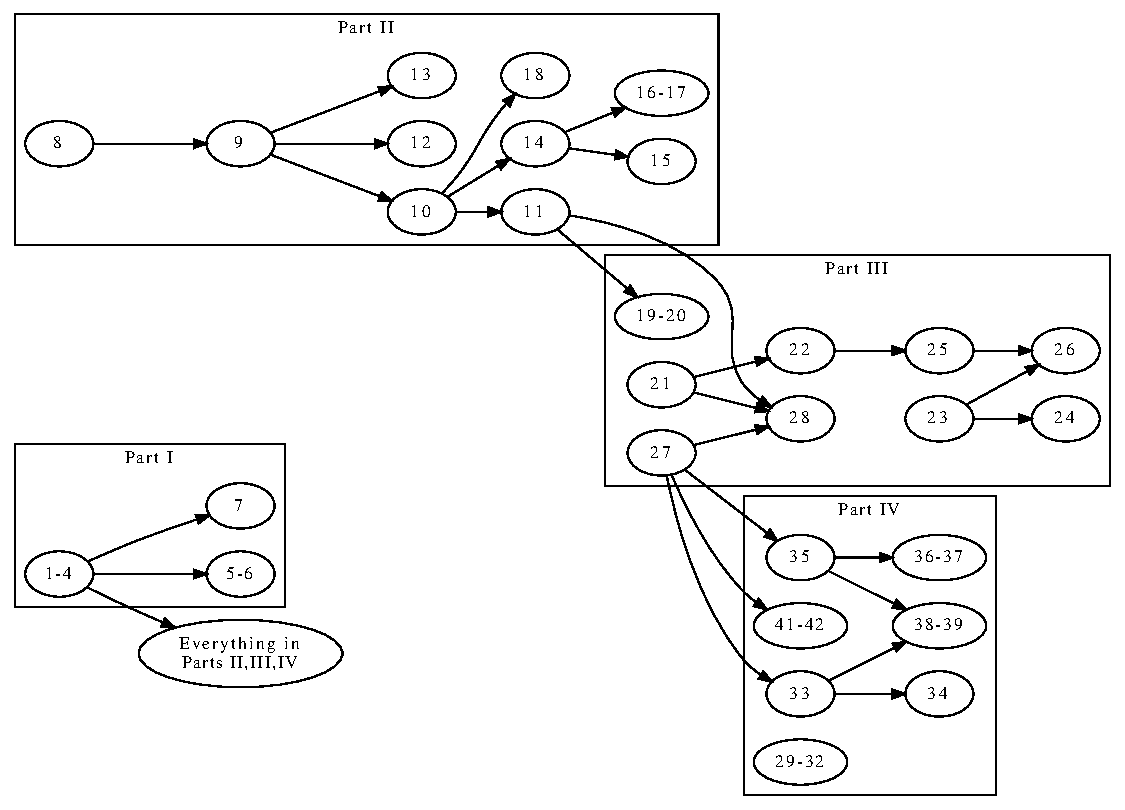
\includegraphics[width=\textwidth]{depend}
\vfill
\tableofcontents



\mainmatter

%%%%%%%%%%%%%%%%%%%%%%%%%%%%%%%%%%%%%%%%%%%%%%%%%%%%%%%%%%%%%
%%%%%%%%%%%%%%%%%%%%%%%%%%%%%%%%%%%%%%%%%%%%%%%%%%%%%%%%%%%%%
%%%%%%%%%%%%%%%%%%%%%%%%%%%%%%%%%%%%%%%%%%%%%%%%%%%%%%%%%%%%%
%%%%%%%%%%%%%%%%%%%%%%%%%%%%%%%%%%%%%%%%%%%%%%

\part{\textsc{Matlab} and Solving Equations}

%%%%%%%%%%%%%%%%%%%%%%%%%%%%%%%%%

\chapter{Vectors, Functions, and  Plots in {\sc Matlab}}
\label{lec:vectors}

In these notes 
\begin{lstlisting}[frame=none,numbers=left,showlines=true]


\end{lstlisting}
will indicate commands to be entered 
at the {\sc Matlab} prompt \(\gg\) in the command window.
You do not type the symbol \(\gg\).

%%%%%%%%%%%%%

\subsection*{Entering vectors}

In \textsc{Matlab}, the basic objects are matrices, i.e.~arrays
of numbers. Vectors can be thought of as special matrices.
A row vector is recorded as a $1 \times n$ matrix
and a column vector is recorded as a $m \times 1$ matrix.
To enter a row vector in Matlab, type the following in the command window:
\begin{lstlisting}[frame=none,numbers=left]
v = [0 1 2 3]
\end{lstlisting}
and press enter. \textsc{Matlab} will print out the row vector.
To enter a column vector type
\begin{lstlisting}[frame=none,numbers=left]
u = [9; 10; 11; 12; 13]
\end{lstlisting}
You can access an entry in a vector with
\begin{lstlisting}[frame=none,numbers=left]
u(2)
\end{lstlisting}
and change the value of that entry with
\begin{lstlisting}[frame=none,numbers=left]
u(2)=47
\end{lstlisting}
You can extract a {\em slice}\ out of a vector with
\begin{lstlisting}[frame=none,numbers=left]
u(2:4)
\end{lstlisting}
You can change a row vector into a column vector, and vice versa,
easily in Matlab using
\begin{lstlisting}[frame=none,numbers=left]
w = v'
\end{lstlisting}
(This is called {\em transposing}\ the vector and we call \verb&'&
the transpose operator.)
There are also useful shortcuts to make vectors such as
\begin{lstlisting}[frame=none,numbers=left]
x = -1:.1:1
y = linspace(0,1,11)
\end{lstlisting}

%%%%%%%%%%%%%

\subsection*{Basic Formatting}

To make \textsc{Matlab} put fewer blank lines in its output, enter
\begin{lstlisting}[frame=none,numbers=left]
format compact
pi
x
\end{lstlisting}
To make \textsc{Matlab} display more digits, enter
\begin{lstlisting}[frame=none,numbers=left]
format long
pi
\end{lstlisting}
Note that this does not change the number of digits \textsc{Matlab} is
using in its calculations; it only changes what is displayed.

%%%%%%%%%%%%%%

\subsection*{Plotting Data}

Consider the data in Table~\ref{tab:viscosity}.\footnote{Adapted from
  Ayyup \&McCuen 1996, p.174.}
\begin{table}[h]
\centerline{
\begin{tabular}{|c|ccccc|}
\hline
 T ($\text{C}^\circ$)  & 5 & 20 & 30 & 50 & 55  \\
  $\mu$ & 0.08 & 0.015 & 0.009 & 0.006 & 0.0055 \\ \hline
\end{tabular}
}
\caption{Viscosity of a liquid as a function of temperature.}
\label{tab:viscosity}
\end{table}
We can enter this data into \textsc{Matlab} with the following
commands entered in the command window:
\begin{lstlisting}[frame=none,numbers=left]
x = [ 5  20  30  50  55 ]
y = [ 0.08  0.015  0.009  0.006  0.0055]
\end{lstlisting}
Entering the name of the variable retrieves its current values.
For instance
\begin{lstlisting}[frame=none,numbers=left]
x
y
\end{lstlisting}
We can plot data in the form of vectors using the plot command:
\begin{lstlisting}[frame=none,numbers=left]
plot(x,y)
\end{lstlisting}
This will produce a graph with the data points connected by lines.  If
you would prefer that the data points be represented by symbols
you can do so. For instance
\begin{lstlisting}[frame=none,numbers=left]
plot(x,y,'*')
plot(x,y,'o')
plot(x,y,'.')
\end{lstlisting}

%%%%%%%%%%%%%%%%

\subsection*{Data as a Representation of a Function}

A major theme in this course is that often we are interested
in a certain function $y = f(x)$, but the only
information we have about this function is a discrete set of data
$\{(x_i,y_i)\}$. Plotting the data, as we did above, can be thought of
envisioning the function using just the data. We will find later
that we can also do other things with the function, like
differentiating and integrating, just using
the available data. Numerical methods, the topic of this course,
means doing mathematics by computer. Since a computer can only store
a finite  amount of information, we will almost always be working
with a finite, discrete set of values of the function (data), rather
than a formula for the function.

%%%%%%%%%%%%%%%%

\subsection*{Built-in Functions}

If we wish to deal with formulas for functions, \textsc{Matlab} contains a
number of built-in functions, including all
the usual functions, such as \verb^sin( )^, \verb^exp( )^, etc.. The meaning
of most of these is clear. The dependent variable (input) always goes
in parentheses in \textsc{Matlab}. For instance
\begin{lstlisting}[frame=none,numbers=left]
sin(pi)
\end{lstlisting}
should return the value of $\sin \pi$, which is of course $0$ and
\begin{lstlisting}[frame=none,numbers=left]
exp(0)
\end{lstlisting}
will return $e^0$, which is $1$.
More importantly, the built-in functions  can operate
not only on single numbers but on vectors. For example
\begin{lstlisting}[frame=none,numbers=left]
x = linspace(0,2*pi,41)
y = sin(x)
plot(x,y)
\end{lstlisting}
will return a plot of $\sin x$ on the interval $[0,2 \pi]$

Some of the built-in functions in \textsc{Matlab} include:
\verb^cos( )^, \verb^tan( )^, \verb^sinh( )^, \verb^cosh( )^,
\verb^log( )^ (natural logarithm), \verb^log10( )^
(log base 10), \verb^asin( )^ (inverse sine), \verb^acos( )^, \verb^atan( )^.
To find out more about a function, use the \verb&help& command; try
\begin{lstlisting}[frame=none,numbers=left]
help plot
\end{lstlisting}

%%%%%%%%%%%%%%%%

\subsection*{User-Defined Anonymous Functions}

If we wish to deal with a function that is a combination of the
built-in functions, \textsc{Matlab} has a couple of ways for the user
to define functions.  One that we will use a lot is the anonymous
function, which is a way to define a function in the command window.
The following is a typical anonymous function:
\begin{lstlisting}[frame=none,numbers=left]
f = @(x) 2*x.^2 - 3*x + 1
\end{lstlisting}
This produces the function $f(x) = 2 x^2 -3x+1$. To obtain a single
value of this function enter
\begin{lstlisting}[frame=none,numbers=left]
y = f(2.23572)
\end{lstlisting}

Just as for built-in functions, the function $f$ as we defined it can
operate
not only on single numbers but on vectors. Try the following:
\begin{lstlisting}[frame=none,numbers=left]
x = -2:.2:2
y = f(x)
\end{lstlisting}
This is an example of {\em vectorization}, i.e.\ putting several
numbers into a vector and treating the vector all at once, rather than
one component at a time, and is one of the strengths of
\textsc{Matlab}.  The reason $f(x)$ works when $x$ is a vector is
because we represented $x^2$ by \verb&x.^2&. The \verb&.& turns the
exponent operator \verb&^& into entry-wise exponentiation, so that
\verb&[-2 -1.8 -1.6].^2& means $[(-2)^2, (-1.8)^2, (-1.6)^2]$ and
yields \verb&[4 3.24 2.56]&.  In contrast, \verb&[-2 -1.8 -1.6]^2&
means the matrix product $[-2, -1.8,-1.6][-2, -1.8,-1.6]$ and yields
only an error. The \verb&.& is needed in \verb&.^&, \verb&.*&, and
\verb&./&. It is not needed when you \verb&*& or \verb&/& by a scalar
or for \verb&+&.

The results can be plotted using the \verb&plot& command, just as for data:
\begin{lstlisting}[frame=none,numbers=left]
plot(x,y)
\end{lstlisting}
Notice that before plotting the function, we in effect converted it
into data. Plotting on any machine always requires this step.


%%%%%%%%%%%%%%%%

\section*{Exercises}
\begin{list}
{\arabic{chapter}.\arabic{exercise}}{\usecounter{exercise}}

\item Recall that \verb&.*&, \verb&./&, \verb&.^& are component-wise operations.
Make row vectors $\mathbf{a} = 0:1:3$ and $\mathbf{b} = [-1 \  \ 0 \  \ 1 \  \ 2]$.
Try the following commands and report the answer (or error) they produce. Are any of the results surprising?

(a)  \verb&a.*b&, \hspace{.2in}    (b)  \verb&a*b&, \hspace{.2in}  (c)  \verb&a*b'&, \hspace{.2in}  (d)  \verb&a+3*b&,  

(e)   \verb&a./b&, \hspace{.2in}    (f)  \verb&2*b./a&,   \hspace{.2in}  (g)  \verb&a.^3&, \hspace{.2in}  (h) \verb&a.^b&,


\item Find a table of data in an engineering or science textbook or 
  website. Input it as vectors and plot it, {\em using symbols at the data points}. 
  
  Use the insert icon to
  label the axes and add a title to your graph. Turn in the graph.
  Indicate what the data is and properly reference where it came from.
  
\item  Find a {\em non-linear} function formula in an engineering or science textbook or 
  website. Make an anonymous function that produces that function. Plot it
  with a {\em smooth curve}  on a physically relevant  domain. 
  
  Label the axes and add a title to your
   graph. Turn in the graph and include the Matlab command for 
   the anonymous function. Indicate what the function means and properly 
   reference where it came from.
   


\end{list}






%%%%%%%%%%%%%%%%%%%%%%%%%%%%%%%%%%%%%%%%%%%%%%%%%%%%%%%%%%%%%%%%%%%%%%%%%%%%

\chapter{{\sc  Matlab} Programs}

In \textsc{Matlab}, programs may be written and saved in files with
a suffix \verb&.m& called {\em M-files}. There are two types of
M-file programs: {\em functions} and {\em scripts}.

%%%%%%%%%%%%%%

\subsection*{Function Programs}

Begin by clicking on the new document icon in the top
left of the \textsc{Matlab} window (it looks like an empty sheet of paper).

In the document window type the following:
\begin{lstlisting}
function y = myfunc(x)
    y = 2*x.^2 - 3*x + 1;
end
\end{lstlisting}

Save this file as: \verb&myfunc.m& in your working directory.
This file can now be used in the command window just like any
predefined Matlab function; in the command window enter:
\begin{lstlisting}[frame=none,numbers=left]
x = -2:.1:2;     % Produces a vector of x values
y = myfunc(x);   % Produces a vector of y values
plot(x,y)
\end{lstlisting}
Note that the fact we used \verb&x& and \verb&y& in both the function
program and in the command window was just a coincidence. In fact, it
is the name of the file \verb&myfunc.m& that actually mattered, not
what anything in it was called.
We could just as well have made the function
\begin{lstlisting}
function nonsense = yourfunc(inputvector)
    nonsense = 2*inputvector.^2 - 3*inputvector + 1;
end
\end{lstlisting}

Look back at the program.
All function programs are like this one, the essential elements are:
\begin{itemize}
\item Begin with the word \verb&function&.
\item There is an input and an output.
\item The output, name of the function and the input must appear in the first line.
\item The body of the program must assign a value to the output variable(s). 
\item The program cannot access variables in the current workspace unless they
           are input.
\item Internal variables inside a function do not appear in the current workspace.
\end{itemize}

Functions can have multiple inputs, which are separated by commas. 
For example:
\begin{lstlisting}
function y = myfunc2d(x,p)
    y = 2*x.^p - 3*x + 1;
end
\end{lstlisting}

Functions can have multiple outputs, which are collected into a vector. 
Open a new document and type:
\begin{lstlisting}
function [x2 x3 x4] = mypowers(x)
    x2 = x.^2;
    x3 = x.^3;
    x4 = x.^4;
end
\end{lstlisting}
Save this file as \verb&mypowers.m&.
In the command window, we can use the results of the program to make graphs:
\begin{lstlisting}[frame=none,numbers=left]
x = -1:.1:1
[x2 x3 x4] = mypowers(x);
plot(x,x,'black',x,x2,'blue',x,x3,'green',x,x4,'red')
\end{lstlisting}

\subsubsection{Printing, Returning, Capturing, and Printing}

Notice that in the examples above, lines ending with a semicolon ``;''
did not print their results.

Try the following:
\begin{lstlisting}[frame=none,numbers=left]
myfunc(3)
ans^2
\end{lstlisting}
Although \verb&myfunc& returned a value, we did not capture it. By
default \textsc{Matlab} captured it as \verb&ans& so we can use it in
our next computation. However, \textsc{Matlab} always uses \verb&ans&
(for answer), so the result is likely to get overwritten.

Then try:
\begin{lstlisting}[frame=none,numbers=left]
z = 0
z = myfunc(2)
z^2
\end{lstlisting}
\verb&myfunc&
returned a value that it internally called \verb&y& and we captured
the result in \verb&z&. We can now use \verb&z& for other calculations.

Now make a program 
\begin{lstlisting}
function myfuncnoreturn(x)
    y = 2*x.^2 - 3*x + 1
end
\end{lstlisting}
and try:
\begin{lstlisting}[frame=none,numbers=left]
myfuncnoreturn(4)
ans^2
y^2
\end{lstlisting}
Although the value of \verb&y& was printed within the function, it was
not returned, so neither the value of \verb&y& nor the value of
\verb&ans& was changed. Thus we cannot use the result from the function.

In general, the best way to use a function is to capture the result
it returns and then use or print this result.
Printing within functions is bad form; however, for
understanding what is happening within a function it is useful to print, so many
functions in this book do print.


%%%%%%%%%%%%%%%%

\subsection*{Script Programs}

\textsc{Matlab} uses a second type of program that differs from
a function program in several ways, namely:
\begin{itemize}
\item There are no inputs and outputs.
\item A script program may use, create  and change variables in the current
  workspace (the variables used by the command window).
\end{itemize}
Below is a script program that accomplishes the same thing as
the function program plus the commands in the previous section:
\begin{lstlisting}
x2 = x.^2;
x3 = x.^3;
x4 = x.^4;
plot(x,x,'black',x,x2,'blue',x,x3,'green',x,x4,'red')
\end{lstlisting}

Type this program into a new document and save it as \verb&mygraphs.m&.
In the command window enter:
\begin{lstlisting}[frame=none,numbers=left]
x = -1:.1:1;
mygraphs
\end{lstlisting}
Note that the program used the variable \verb&x& in its calculations, even
though \verb&x& was defined in the command window, not in the program.

Many people use script programs for routine calculations that
would require typing more than one
command in the command window. They do this because correcting
mistakes is easier in a program than in the command window.

%%%%%%%%%%%%%%%%

\subsection*{Program Comments}

For programs that have more than a couple of lines it
is important to include comments. Comments allow other
people to know what your program does and they also
remind yourself what your program does if you set it
aside and come back to it later. It is best to include
comments not only at the top of a program, but also
with each section. In \textsc{Matlab} anything that
comes in a line after a \verb&%& 
is a comment.

For a function program, the comments should at least give the purpose,
inputs, and outputs. A properly commented version of the function with
which we started this section is:
\begin{lstlisting}
function y = myfunc(x)
    % Computes the function 2x^2 -3x +1
    % Input: x -- a number or vector; 
    %             for a vector the computation is elementwise
    % Output: y -- a number or vector of the same size as x
    y = 2*x.^2 - 3*x + 1;
end
\end{lstlisting}

For a script program, there should be an initial comment stating the purpose of the script.
It is also  helpful to include the name of the program at the beginning.
For example:
\begin{lstlisting}
% mygraphs
% plots the graphs of x, x^2, x^3, and x^4
% on the interval [-1,1]

% fix the domain and evaluation points
x = -1:.1:1;

% calculate powers
% x1 is just x
x2 = x.^2;
x3 = x.^3;
x4 = x.^4;

% plot each of the graphs
plot(x,x,'+-',x,x2,'x-',x,x3,'o-',x,x4,'--')
\end{lstlisting}

The \textsc{Matlab} command \verb&help& prints the first block of
comments from a file. If we save the above as \verb&mygraphs.m& and
then do
\begin{lstlisting}[frame=none,numbers=left]
help mygraphs
\end{lstlisting}
it will print into the command window:
\begin{lstlisting}[frame=none,numbers=left]
mygraphs
plots the graphs of x, x^2, x^3, and x^4
on the interval [-1,1]
\end{lstlisting}

%%%%%%%%%%%%%%%%

\section*{Exercises}

\begin{list}
{\arabic{chapter}.\arabic{exercise}}{\usecounter{exercise}}
\item Write a well-commented {\bf function} program for the function
  $x^2 e^{-x^2}$, using component-wise operations (such as \verb&.*&
  and~\verb&.^&). To get $e^x$ use \verb&exp(x)&.  Plot the function
  on $[-5,5]$ using enough points to make the graph smooth. Turn in
  the program and the graph.
%(The graph of
%      the function $e^{-x^2}$ is the bell-curve that is used
%      in probability and statistics.)

\item Write a well-commented {\bf script} program that graphs the
  functions $\sin x$, $\sin 2x$, $\sin 3x$, $\sin 4x$, $\sin 5x$ and
  $\sin 6x$ on the interval $[0, 2\pi]$ on one plot. ($\pi$ is
  \verb&pi& in \textsc{Matlab}.) Use a sufficiently small step size to
  make all the graphs smooth. 
  Turn in the program and the graph.
\end{list}





%%%%%%%%%%%%%%%%%%%%%%%%%%%%%%%%%%%%%%%%%%%%%%%%


\chapter{Newton's Method and Loops}
\label{lec:newton}

%%%%%%%%%%%%%%%%

\subsection*{Solving equations numerically}

For the next few lectures we will focus on the problem of solving an
equation:
\begin{equation}\label{fzero}
     f(x) = 0.
\end{equation}
As you learned in calculus, the final step in many optimization
problems is to solve an equation of this form where $f$ is the
derivative of a function, $F$, that you want
to maximize or minimize. In real engineering problems the
functions, $f$, you wish to find roots for can come from a large variety of
sources, including formulas, solutions of differential equations, experiments,
or simulations.


%%%%%%%%%%%%%%%%

\subsection*{Newton iterations}

We will denote an actual solution of equation (\ref{fzero}) by $x^*$.
There are three methods that you may have discussed in Calculus:
the bisection method, the secant method and Newton's method. All
three depend on beginning close (in some sense) to an actual solution
$x^*$.

Recall Newton's method. You should know that the basis for
Newton's method is approximation of a function by its linearization
at a point, i.e.
\begin{equation}\label{linapp}
f(x) \approx f(x_0) + f'(x_0)(x-x_0).
\end{equation}
Since we wish to find $x$ so that $f(x) =0$, set the left hand side ($f(x)$)
of this approximation equal to $0$ and solve for $x$ to obtain:
\begin{equation}\label{newtona}
x \approx x_0 - \frac{f(x_0)}{f'(x_0)}.
\end{equation}
We begin the method with the initial guess
$x_0$, which we hope is fairly close to $x^*$.
Then we define a sequence of points $\{x_0, x_1, x_2, x_3, \ldots \}$
from the formula:
\begin{equation}\label{newton}
x_{i+1} = x_i - \frac{f(x_i)}{f'(x_i)},
\end{equation}
which comes from (\ref{newtona}).
If $f(x)$ is reasonably well-behaved near $x^*$ and $x_0$ is
close enough to $x^*$, then it is a fact that the sequence will
converge to $x^*$ and will do it very quickly.


%%%%%%%%%%%%%%%%

\subsection*{The loop: \texttt{for ... end}}

In order to do Newton's method, we need to repeat the
calculation in (\ref{newton}) a number of times. This
is accomplished in a program using a {\em loop}, which
means a section of a program which is repeated. The simplest
way to accomplish this is to count the number of times
through. In \textsc{Matlab}, a \verb&for ... end& statement makes a loop
as in the following simple function program:
\begin{lstlisting}
    % mysum
    % Gives the sum of the first n integers   
    %
    n = 100            
    S = 0;            % start at zero
    % The loop:
    for i = 1:n       % do n times
        S = S + i;    % add the current integer
    end               % end of the loop
    S
\end{lstlisting}

Save this program as a {\bf script} named \verb& mysum & and
run it by typing \verb& mysum & in the command window.
The result will be the sum of the first 100 integers.
Next change $n$ to 1,000,000 and run the program again.

All \verb&for ... end& loops have the same format, it begins
with \verb&for&, followed by an index (\verb&i&) and a range of numbers
(\verb&1:n&). Then
come the commands that are to be repeated. Last comes
the \verb&end& command.

Loops are one of the main ways that computers are made
to do calculations that humans cannot. Any calculation
that involves a repeated process is easily done by
a loop.

Now let's do a program that does n steps (iterations)
of Newton's method.
We will need to input the function, its derivative, the initial
guess, and the number of steps. The output will be the final
value of $x$, i.e.~$x_n$. If we are only interested in the
final approximation, not the intermediate steps, which is
usually the case in the real world, then we can use a single
variable \verb&x& in the program \programlink{mynewton.m} and change it at each step:
\lstinputlisting{../programs/mynewton.m}

In the command window set to print more digits via
\begin{lstlisting}[frame=none,numbers=left]
format long
\end{lstlisting}
and to not print blank lines via
\begin{lstlisting}[frame=none,numbers=left]
format compact
\end{lstlisting}
Then define a function: $f(x) = x^3 - 5$
i.e.
\begin{lstlisting}[frame=none,numbers=left]
f = @(x) x^3 - 5
\end{lstlisting}
and define $f1$ to be its derivative, i.e.
\begin{lstlisting}[frame=none,numbers=left]
f1 = @(x) 3*x^2
\end{lstlisting}
Then run \verb&mynewton& on this function.
By trial and error, what is the lowest value of \verb&n& for which the
program converges (stops changing).  By simple algebra, the true root
of this function is $\sqrt[3]{5}$. How close is the program's answer
to the true value?

%%%%%%%%%%%%

\subsection*{Convergence}

Newton's method converges rapidly when $f'(x^*)$ is nonzero and
finite, and $x_0$ is close enough to $x^*$ that the  linear approximation
(\ref{linapp}) is valid.
Let us take a look at what can go wrong.

For $f(x)=x^{1/3}$ we have $x^*=0$ but $f'(x^*)=\infty$.  If you try
\begin{lstlisting}[frame=none,numbers=left]
f = @(x) x^(1/3)
f1 = @(x) (1/3)*x^(-2/3)
x = mynewton(f,f1,0.1,10)
\end{lstlisting}
then $x$ explodes.

For $f(x)=x^2$ we have $x^*=0$ but $f'(x^*)=0$.  If you try
\begin{lstlisting}[frame=none,numbers=left]
f = @(x) x^2
f1 = @(x) 2*x
x = mynewton(f,f1,1,10)
\end{lstlisting}
then $x$ does converge to $0$, but not that rapidly.

If $x_0$ is not close enough to $x^*$ that the linear approximation
(\ref{linapp}) is valid, then the iteration (\ref{newton}) gives some
$x_1$ that may or may not be any better than $x_0$. If we keep iterating,
then either
\begin{itemize}
\item
$x_n$ will eventually get close to $x^*$ and the method will then
converge (rapidly), or
\item
the iterations will not approach $x^*$.
\end{itemize}
%
%To see the second case try:\\
%\verb& > f = inline('x^(1/3) - 1')&\\
%\verb& > f1 = inline('(1/3)*x^(-2/3)')&\\
%The obvious solution of $x^{1/3} - 1 = 0$ is $1$.
%If we try $x_0$ close to $1$, the program will produce
%the correct answer in only a few steps.\\
%\verb& > x = mynewton(f,f1,2,10)&\\
%If, however, you choose $x_0$ far from $1$ even a large number of
%iterations will not produce the desired result:\\
%\verb& > x = mynewton(f,f1,10,10)&


%%%%%%%%%%%%%%%%%%%%%%%
\newpage
\subsection*{Exercises}

\nobreak \begin{list}
{\arabic{chapter}.\arabic{exercise}}{\usecounter{exercise}}


   
\item Enter: \verb&format long&.  Use \programlink{mynewton.m} on the function
  $f(x) = x^5 - 2$, with $x_0 = 1$. By trial and error, what is the
  lowest value of \verb&n& for which the program converges (stops
  changing). Compute the error, which is how close the program's
  answer is to the true value. Compute the residual, which is the
  program's answer plugged into $f$. (See the next section for discussion.) 
  Are the error and residual zero?
   
\item For $f(x) = x^2 - 5$, perform 3 iterations of Newton's method
  with starting point $x_0 = 2$. (By hand, but use a calculator.) Show all
  steps.
  Calculate the solution ($x^* = \sqrt{5}$) on a calculator and find
  the errors and percentage errors of $x_0$, $x_1$, $x_2$ and $x_3$.
  Use enough digits so that you do not falsely conclude the error is
  zero. 
  \label{exr:newtonbyhand}


\item Suppose a ball is dropped from a height of 3 meters onto a hard
  surface and the coefficient of restitution of the collision is .91
  (see Wikipedia for an explanation).  Write a well-commented {\bf
    script} program to calculate the total distance the ball has
  traveled when it hits the surface for the \verb&n&-th time.  Enter:
  \verb&format long&. By trial and error approximate how large
  \verb&n& must be so that total distance stops changing. Turn in the
  program and a brief summary of the results. (This program does not
  use Newton's method. It should be modeled on \verb&mysum.m&.)
  \label{exr:bounce}


\end{list}




%%%%%%%%%%%%%%%%%%%%%%%%%%%%%%%%%%%%%%%%%%%%%%%%%%%%%%%%%%%%%%%

\chapter{Controlling Error and Conditional Statements}

%%%%%%%%%%%%%%%%

\subsection*{Measuring error and the Residual}

If we are trying to find a numerical solution of an equation
$f(x) = 0$, then there are a few different ways we can measure
the error of our approximation. The most direct way to
measure the error would be as
$$
   \{ \text{Error at step $n$} \} = e_n = x_n - x^*
$$
where $x_n$ is the $n$-th approximation and $x^*$ is the true
value. However, we usually do not know the value of $x^*$, or
we wouldn't be trying to approximate it. This makes
it impossible to know the error directly, and so we must be
more clever.

One possible strategy, which often works,  is to
run a program until the approximation $x_n$ stops changing.
The problem with this is that it sometimes doesn't work. Just because the
program stop changing does not necessarily mean that $x_n$ is
close to the true solution.

For Newton's method we have the following principle:
{\bf At each step the number of significant digits roughly
doubles.}
While this is an important statement about the error
(since it means Newton's method
converges really quickly), it is somewhat hard to use in a
program.

Rather than measure how close $x_n$ is to $x^*$, in this and many other
situations it is much more practical to measure how close the equation
is to being satisfied, in other words, how close $y_n = f(x_n)$ is to $0$.
We will use the quantity $r_n =  f(x_n)-0$, called the {\em residual},
in many different situations. Most of the time we only care about the
size of $r_n$, so we use the absolute value of the residual as a measure
of how close the solution is to solving the problem:
$$
  |r_n|=|f(x_n)|.
$$



%%%%%%%%%%%%%%%%

\subsection*{The \texttt{if ... end} statement}

If we have a certain tolerance
for $|r_n| = |f(x_n)|$, then we can incorporate that into our Newton method
program using an \verb&if ... end& statement:
\begin{lstlisting}
function x = mynewton(f,f1,x0,n,tol)
    % Solves f(x) = 0 by doing n steps of Newton's method starting at x0.
    % Inputs: f -- the function
    %         f1 -- it's derivative
    %         x0 -- starting guess, a number
    %         tol -- desired tolerance, prints a warning if |f(x)|>tol
    % Output: x -- the approximate solution
    x = x0;                   % set x equal to the initial guess x0
    for i = 1:n               % Do n times
        x = x - f(x)/f1(x)  % Newton's formula
    end
    r = abs(f(x))
    if r > tol
        warning('The desired accuracy was not attained')
    end
end
\end{lstlisting}


In this program \verb&if& checks if \verb&abs(y) > tol&
is true or not. If it is true then it does everything
between there and \verb&end&. If not true, then it skips
ahead to \verb&end&.

In the command window define a function and its derivative:
\begin{lstlisting}[frame=none,numbers=left]
f = @(x) x^3-5
f1 = @(x) 3*x^2
\end{lstlisting}
Then use the program with $n=3$, $tol = .01$, and $x_0=2$.
Next, change $tol$ to $10^{-10}$ and repeat.

%%%%%%%%%%%%%%%%

\subsection*{The loop: \texttt{while ... end}}

While the previous program will tell us if it worked or not,
we still have to input \verb&n&, the number of steps to take.
Even for a well-behaved problem, if we make \verb&n& too small
then the tolerance will not be attained and we will have to
go back and increase it, or, if we make \verb&n& too big, then
the program will take more steps than necessary.

One way to control the number of steps taken is to iterate
until the residual $|r_n| = |f(x)| = |y|$ is small enough.
In \textsc{Matlab} this is easily accomplished with a
\verb&while ... end& loop.
\begin{lstlisting}
function x = mynewtontol(f,f1,x0,tol)
    % Solves f(x) = 0 using Newton's method until |f(x)| < tol.
    % Inputs: f -- the function
    %         f1 -- it's derivative
    %         x0 -- starting guess, a number
    %         tol -- desired tolerance, runs until |f(x)|<tol
    % Output: x -- the approximate solution
    x = x0;                   % set x equal to the initial guess x0
    y = f(x);
    while abs(y) > tol     % Do until the tolerence is reached.
        x = x - y/f1(x)    % Newton's formula
        y = f(x)
    end
end
\end{lstlisting}


The statement \verb&while ... end& is a loop,
similar to \verb&for ... end&, but instead of going through the
loop a fixed number of times it keeps going as long as the statement
\verb&abs(y) > tol & is true.

One obvious drawback of the program is that \verb&abs(y)& might
never get smaller than \verb&tol&. If this happens, the program
would continue to run over and over until we stop it. Try this
by setting the tolerance to a really small number:
\begin{lstlisting}[frame=none,numbers=left]
tol = 10^(-100)
\end{lstlisting}
then run the program again for $f(x) = x^3 - 5$.
(You can use \verb&Ctrl-c& to stop a program when it is stuck.)

One way to avoid an infinite loop is add a counter variable, say
\verb& i & and a maximum number of iterations to the programs.
Using the \verb& while & statement, this can be accomplished as:
\begin{lstlisting}
function x = mynewtontol(f,f1,x0,tol)
    % Solves f(x) = 0 using Newton's method until |f(x)| < tol.
    %     Safety stop after 1000 iterations
    % Inputs: f -- the function
    %         f1 -- it's derivative
    %         x0 -- starting guess, a number
    %         tol -- desired tolerance, runs until |f(x)|<tol 
    % Output: x -- the approximate solution
    x = x0;    % set x equal to the initial guess x0. 
    i=0;       % set counter to zero 
    y = f(x);
    while abs(y) > tol & i < 1000  
        % Do until the tolerence is reached or max iter.
        x = x - y/f1(x)    % Newton's formula
        y = f(x)
        i = i+1;           % increment counter
    end
end
\end{lstlisting}


\newpage
%%%%%%%%%%%%%%%%

\subsection*{Exercises}

\nobreak
\begin{list}
{\arabic{chapter}.\arabic{exercise}}{\usecounter{exercise}}

\item In Calculus we learn that a geometric series has an exact sum
$$
   \sum_{i=0}^\infty r^i = \frac{1}{1-r}
   \,,
$$
provided that $|r|<1$. For instance, if $r = .5$ then the sum is
exactly $2$.  Below is a script program that lacks one line as
written.  Put in the missing command and then use the program to
verify the result above. How many steps does it take? How close is the
answer to $2$?
\begin{lstlisting}
% Computes a geometric series until it seems to converge
format long
format compact
r = .5;
Snew = 0;           % start sum at 0
Sold = -1;          % set Sold to trick while the first time
i = 0;              % count iterations
while Snew > Sold   % is the sum still changing?
   Sold = Snew;     % save previous value to compare to
   Snew = Snew + r^i;
   i=i+1;
Snew                % prints the final value.
i                   % prints the # of iterations.
\end{lstlisting}
Add a line at the end of the program to compute the error of
\verb&Snew& (with respect to the exact value from the formula above). 
Run the script for $r=0.9$, 0.99, 0.999, 0.9999, 0.99999, and 0.999999. 
Turn in your program and a table showing the approximate sum, number of iterations needed and the error for each $r$.


\item Modify your program from exercise
  \ref{lec:newton}.\ref{exr:bounce} to compute the total distance
  traveled by the ball while its bounces are at least  $0.01$ millimeter
  high. Use a \verb&while& loop (instead of  \verb&for&)  to decide when to stop summing (do not
  use a \verb&for& loop or trial and error). Turn in your modified program and
  a brief summary of the results.

\end{list}



%%%%%%%%%%%%%%%%%%%%%%%%%%%%%%%%%%%%%%%%%%%%%%%%%%%%%%%%%%%%%%%

\chapter{The Bisection Method and Locating Roots}
\label{lec:bisection}

%%%%%%%%%%%%%%%%

\subsection*{Bisecting and the \texttt{if ... else ... end} statement}

Recall the bisection method. Suppose that $c = f(a) < 0$ and
$d = f(b) > 0$. If $f$ is continuous, then obviously
it must be zero at some $x^*$ between $a$ and $b$.
The bisection method then consists of looking half
way between $a$ and $b$ for the zero of $f$, i.e. let
$x = (a+b)/2$ and evaluate $y = f(x)$. Unless this is
zero, then from the signs of $c$, $d$ and $y$ we can decide
which new interval to subdivide. In particular, if $c$ and $y$
have the same sign, then $[x,b]$ should be the new interval,
but if $c$ and $y$ have different signs, then $[a,x]$ should
be the new interval. (See Figure~\ref{bisecfig}.)


\begin{figure}[h]
\setlength{\unitlength}{2 mm}
%\LARGE
\begin{center}
\begin{picture}(64,20)(0,-12)
	\put(0,0){\line(1,0){64}}
	\put(0,-2){\line(0,1){4}}
	\put(64,-2){\line(0,1){4}}
	\put(32,-2){\line(0,1){4}}
	\put(16,-2){\line(0,1){4}}
	\put(24,-2){\line(0,1){4}}
	\put(32,-4){\mbox{$x_0$}}
	\put(16,-4){\mbox{$x_1$}}
	\put(24,-4){\mbox{$x_2$}}
	\put(0,-4){\mbox{$a_0$}}
	\put(64,-4){\mbox{$b_0$}}
	\put(0,-7){\mbox{$a_1$}}
	\put(32,-7){\mbox{$b_1$}}
	\put(16,-10){\mbox{$a_2$}}
	\put(32,-10){\mbox{$b_2$}}
	\put(0,-12){\circle*{1}}
	\put(64,8){\circle*{1}}
	\put(32,4){\circle*{1}}
	\put(16,-7){\circle*{1}}
\end{picture}
\end{center}
\caption{The bisection method.}
\label{bisecfig}
\end{figure}

Deciding to do different things in different situations in
a program is called {\em flow control}. The most common way
to do this is the \verb&if ... else ... end& statement which
is an extension of the \verb&if ... end& statement we have used
already.

%%%%%%%%%%%%%%%%

\subsection*{Bounding the Error}

One good thing about the bisection method, which we do not
have with Newton's method, is that we always know that
the actual solution $x^*$ is inside the current interval
$[a,b]$, since $f(a)$ and $f(b)$ have different signs.
This allows us to be sure about what the maximum error can be.
Precisely, the error is
always less than half of the length of the current interval
$[a,b]$, i.e.
$$
 \{ \text{Absolute Error} \} = | x - x^* | < (b - a)/2,
$$
where $x$ is the center point between the current $a$ and $b$.

The following function program (available to download as \programlink{mybisect.m})
does $n$ iterations of
the bisection method and returns not only the final value,
but also the maximum possible error:
\lstinputlisting{../programs/mybisect.m}

Another important aspect of bisection is that it always works.
We saw that Newton's method can fail to converge to $x^*$
if $x_0$ is not close enough to $x^*$. In contrast, the current
interval $[a,b]$  will always be decreased by a factor
of 2 at each step and so it will always eventually shrink down as
small as you wish.

%%%%%%%%%%%%%

\subsection*{Locating the roots (if any)}

The bisection method and Newton's method are both used
to obtain closer and closer approximations of a solution,
but both require starting places. The bisection method
requires two points $a$ and $b$ that have a root between
them, and Newton's method requires one point $x_0$ which
is reasonably close to a root. How do you come
up with these starting points? It depends. If you are solving
an equation once, then the best thing to do first is
to just graph it. From an accurate graph you can see approximately
where the graph crosses zero.

There are other situations where you are not just solving
an equation once, but have to solve the same equation many
times, but with different coefficients. This happens often
when you are developing software for a specific application.
In this situation the first thing you want to take advantage
of is the natural domain of the problem, i.e.~on what interval
is a solution physically reasonable. If that is known, then
it is easy to get close to the root by simply checking the
sign of the function at a fixed number of points inside the
interval. Whenever the sign changes from one point to the
next, there is a root between those points. The following
program will look for the roots of a function $f$ on a specified
interval $[a_0,b_0]$.
\begin{lstlisting}
function [a,b] = myrootfind(f,a0,b0)
    % function [a,b] = myrootfind(f,a0,b0)
    % Looks for subintervals where the function changes sign
    % Inputs: f -- a function
    %         a0 -- the left edge of the domain
    %         b0 -- the right edge of the domain
    % Outputs: a -- an array, giving the left edges of subintervals
    %               on which f changes sign
    %          b -- an array, giving the right edges of the subintervals
    n = 1001;   % number of test points to use
    a = [];     % start empty array
    b = [];
    % split the interval into n-1 intervals and evaluate at the break points
    x = linspace(a0,b0,n);
    y = f(x);
    % loop through the intervals
    for i = 1:(n-1)
        if y(i)*y(i+1) <= 0  % The sign changed, record it
            a = [a x(i)];
            b = [b x(i+1)];
        end
    end
    if size(a,1) == 0
        warning('no roots were found')
    end
end
\end{lstlisting}

To see this program in action try the following:
\begin{lstlisting}
f = @(x) sin(x)-2*x.^4+0.5
x = -1:.01:1;
y = f(x);
plot(x,y)     % see that there are two roots
[a,b] = myrootfind(f,-1,1)  % observe that it finds two roots
\end{lstlisting}

The final situation is writing a program that will look
for roots with no given information. This is a difficult
problem and one that is not often encountered in actual 
applications.

Once a root has been located on an interval $[a,b]$,
these $a$ and $b$ can serve as the beginning points
for the bisection and secant methods (see the next section).
For Newton's method one would want to choose $x_0$ between $a$ and
$b$. One obvious choice would be to let $x_0$
be the bisector of $a$ and $b$, i.e.~$x_0 = (a+b)/2$.
An even better choice would be to use the secant method
to choose $x_0$.

%%%%%%%%%%%%%%%
\subsection*{Exercises}

\begin{list}
{\arabic{chapter}.\arabic{exercise}}{\usecounter{exercise}}

\item Modify \verb&mybisect& to solve until the absolute
      error is bounded by a given tolerance. Use a \verb&while& loop to
      do this. 
	Run your
      program on the function $f(x) = 2x^3 + 3x -1$
      with starting interval $[0,1]$ and a tolerance
      of $10^{-8}$. How many steps
      does the program use to achieve this tolerance?
      (You can count the steps by adding $1$ to a counting
      variable \verb&i& in the loop of the program.)
      How big is the final residual $f(x)$?
      Turn in your program and a brief summary of the results.
      \label{exr:bisectionprogram}

\item Perform 3 iterations of the bisection method
      on the function $f(x) = x^2-5$, with starting
      interval $[1,3]$. (By hand, but use a calculator.)
      Calculate the errors and percentage errors of
      $x_0$, $x_1$, $x_2$, and $x_3$. Compare the errors
      with those in exercise \ref{lec:newton}.\ref{exr:newtonbyhand}.
      \label{exr:bisectionbyhand}
      % need to go to x_3 for comparisons
\end{list}



%%%%%%%%%%%%%%%%%%%%%%%%%%%%%%%%%%%%%%%%%%%%%%%%%%%%%%%%

\chapter{Secant Methods}

In this lecture we introduce two additional methods
to find numerical solutions of the equation $f(x) = 0$.
Both of these methods are based on approximating the function
by secant lines just as Newton's method was based on
approximating the function by tangent lines.

%%%%%%%%%%%%%%%%

\subsection*{The Secant Method}

The secant method requires two initial approximations $x_0$ and $x_1$,
preferably both reasonably close to the solution $x^*$.  From $x_0$
and $x_1$ we can determine that the points $(x_0,y_0=f(x_0))$ and
$(x_1,y_1=f(x_1))$ both lie on the graph of $f$. Connecting these
points gives the (secant) line
\[
y - y_1 = \frac{y_1 - y_0}{x_1 - x_0}(x-x_1)
\,.
\]
Since we want $f(x)=0$, we set $y=0$, solve for $x$, and use that as
our next approximation. Repeating this process gives us the iteration
\begin{equation}\label{secant}
x_{i+1} = x_i - \frac{x_i - x_{i-1}}{y_i - y_{i-1}} y_i
\end{equation}
with $y_i=f(x_i)$.
See Figure~\ref{fig:secant} for an illustration.
\begin{figure}[h!]
\begin{center}
\setlength{\unitlength}{1 mm}
\begin{picture}(100,60)(0,-20)
% axis
\put(0,0){\line(1,0){100}}
% curve
\qbezier(0,-20)(60,-20)(100,40)
% initial x
\put(10,-1){\line(0,1){2}}
\put(10,-20){\circle*{2}}
\put(8,-5){\mbox{$x_{i}$}}
\put(90,-1){\line(0,1){2}}
\put(90,27){\circle*{2}}
\put(88,-5){\mbox{$x_{i-1}$}}
% secant
\qbezier(10,-20)(55,6.5)(100,33)
% new point
\put(44,-1){\line(0,1){2}}
\put(42,-5){\mbox{$x_{i+1}$}}
\end{picture}
\end{center}
\caption{The secant method in the case where the root is bracketed.}
\label{fig:secant}
\end{figure}

For example, suppose $f(x) = x^4-5$, which has a solution $x^* =
\sqrt[4]{5}\approx 1.5$. Choose $x_0=1$ and $x_1 = 2$ as initial
approximations.
Next we have that
$y_0 = f(1) = -4$ and $y_1 = f(2) = 11$. We may then calculate
$x_2$ from the formula (\ref{secant}):
$$
x_2 = 2 - \frac{2-1}{11-(-4)} \, 11 = \frac{19}{15} \approx 1.2666... .
$$
Pluggin $x_2 = 19/15$ into $f(x)$ we obtain
$y_2 = f(19/15) \approx -2.425758...$.
In the next step we would use $x_1 = 2$ and $x_2 = 19/15$ in the formula
(\ref{secant}) to find $x_3$ and so on.


Below is a program for the secant method (available to download as \programlink{mysecant.m}). Notice that it requires
two input guesses $x_0$ and $x_1$, but it does not require the derivative
to be input.
\lstinputlisting{../programs/mysecant.m}


%%%%%%%%%%%%%%%%

\subsection*{The {\em Regula Falsi} (False Position) Method}

The {\em Regula Falsi} method is a combination of the secant
method and bisection method.  As in the bisection method, we have to
start with two approximations $a$ and $b$ for which $f(a)$ and $f(b)$
have different signs. As in the secant method, we follow the secant
line to get a new approximation, which gives a formula similar to
(\ref{secant}),
\begin{equation*}
  x = b - \frac{b - a}{f(b) - f(a)} f(b)
  \,.
\end{equation*}
Then, as in the bisection method, we check the sign of $f(x)$; if it
is the same as the sign of $f(a)$ then $x$ becomes the new $a$ and
otherwise let $x$ becomes the new $b$.  Note that in general either
$a\rightarrow x^*$ or $b\rightarrow x^*$ but not both, so $b-a
\not\rightarrow 0$. For example, for the function in
Figure~\ref{fig:secant}, $a\rightarrow x^*$ but $b$ would never move.


%%%%%%%%%%%%%%%%

\subsection*{Convergence}

If we can begin with a good choice $x_0$, then Newton's
method will converge to $x^*$ rapidly. The secant method
is a little slower than Newton's method and the {\em Regula
Falsi} method is slightly slower than that. However, both
are still much faster than the bisection method.

If we do not have a good starting point or interval, then
the secant method, just like Newton's method, can fail altogether.
The {\em Regula Falsi} method, just like the bisection method,
always works because it keeps the solution inside a definite
interval.


%%%%%%%%%%%%%%%%

\subsection*{Simulations and Experiments}

Although Newton's method converges faster than any other
method, there are contexts when it is not convenient,
or even impossible. One obvious situation is when it
is difficult to calculate a formula for $f'(x)$
even though one knows the formula for $f(x)$. This is
often the case when $f(x)$ is not defined explicitly,
but implicitly. There are other situations, which are
very common in engineering and science, where even a formula for
$f(x)$ is not known. This happens when $f(x)$
is the result of experiment or simulation rather than
a formula. In such situations, the secant method is usually
the best choice.

%%%%%%%%%%%%%%%%

\subsection*{Exercises}
\begin{list}
{\arabic{chapter}.\arabic{exercise}}{\usecounter{exercise}}


\item Perform 3 iterations of the secant method
      on the function $f(x) = x^2-5$, with starting
       points $x_{-1} = 1$ and $x_0 =3$. (By hand, but use a calculator.)
      Calculate the errors and percentage errors of
      $x_1$, $x_2$, and $x_3$. Compare the errors
      with those in exercise \ref{lec:newton}.\ref{exr:newtonbyhand}  and
       \ref{lec:bisection}.\ref{exr:bisectionbyhand}.
      \label{exr:secantbyhand}
      
      
\item Create and graph the function \verb& g = @(x) log(x)+x.^2 &.
 In the plot window, use the Tools menu to zoom in on the root (there is only one)
 to 2 decimal places.
 From this determine good starting points \verb&a0& and \verb&b0& and use
 the program \programlink{mysecant.m}  to approximate the root $x^*$ to 15 decimal places. 
 Turn in your zoomed-in plot and your approximation.

%    \item Perform 3 iterations of the {\em Regula Falsi} method on the
%      function $f(x) = x^3 - 4$, with starting interval $[1,3]$. (By
%      hand, but use a calculator.)  Calculate the errors and
%      percentage errors of $x_1$, $x_2$, and $x_3$. Compare the errors
%      with those in exercises \ref{lec:newton}.\ref{exr:newtonbyhand}
%      and \ref{lec:bisection}.\ref{exr:bisectionbyhand}.
%  \label{exr:regulafalsibyhand}
  
  
\item Modify the program \programlink{mysecant.m} to iterate until the
  absolute value of the residual is less than a given tolerance. (Let
  \verb&tol& be an input instead of \verb&n&.) Modify the comments
   appropriately.  Test program on the two functions in the exercises 
   above with \verb&tol& $= 10^{-10}$. Turn in the results and the program.

%\item Write a function program \verb&myregfalsi& that runs the {\em
%    Regula Falsi} method until the absolute value of the residual
%  is below a given tolerance.  Run your program on the function
%  $f(x) = 2x^3 + 3x -1$ with starting interval $[0,1]$ and a tolerance
%  of $10^{-8}$.  How many steps does the program use to achieve this
%  tolerance?  Compare with exercise
%  \ref{lec:bisection}.\ref{exr:bisectionprogram}.  Turn in your
%  program and a brief summary of the results.

% \item Use the program \programlink{mysecant.m} on $f(x) = x^3 - 4$. Compare the
%   results with those of Exercises
%   \ref{lec:newton}.\ref{exr:newtonbyhand} and
%   \ref{lec:bisection}.\ref{exr:bisectionbyhand}. Then modify the
%   program to accept a tolerance using a \verb& while & loop.  Test the
%   program and turn in the program as well as the work above.

\end{list}




%%%%%%%%%%%%%%%%%%%%%%%%%%%%%%%%%%%%%%%%%%%%%%%%%%%%%%%%%%%%%%%%%

\chapter{Symbolic Computations}

The focus of this course is on {numerical} computations, i.e.
calculations, usually approximations, with floating point numbers.
However, \textsc{Matlab}
can also do {\em symbolic} computations, which means exact
calculations using symbols as in Algebra or Calculus.

Note: To do symbolic computations in \textsc{Matlab} one must
have the Symbolic Toolbox.

%%%%%%%%%%%%%%%%

\subsection*{Defining functions and basic operations}

Before doing any symbolic computation, one must declare the
variables used to be symbolic:
\begin{lstlisting}[frame=none,numbers=left]
syms x y
\end{lstlisting}
An expression representing a function may be defined by simply typing the formula:
\begin{lstlisting}[frame=none,numbers=left]
f = cos(x) + 3*x^2
\end{lstlisting}
Note that coefficients must be multiplied using \verb&*&.
To find specific values, you must use the command \verb&subs&:
\begin{lstlisting}[frame=none,numbers=left]
subs(f,pi)
\end{lstlisting}
This command stands for {\em substitute}, it substitutes $\pi$ for $x$
in the formula for $f$.
%
If we define another function:
\begin{lstlisting}[frame=none,numbers=left]
g = exp(-y^2)
\end{lstlisting}
then we can compose the functions:
\begin{lstlisting}[frame=none,numbers=left]
h = compose(g,f)
\end{lstlisting}
i.e. $h(x) = g(f(x))$.
We can also form new functions by multiplying:
\begin{lstlisting}[frame=none,numbers=left]
yg = y*g
\end{lstlisting}

We can do simple calculus operations, like differentiation:
\begin{lstlisting}[frame=none,numbers=left]
f1 = diff(f)
h1 = diff(h)
\end{lstlisting}
indefinite integrals (antiderivatives):
\begin{lstlisting}[frame=none,numbers=left]
F = int(f)
\end{lstlisting}
and definite integrals:
\begin{lstlisting}[frame=none,numbers=left]
int(f,0,2*pi)
\end{lstlisting}
To change a symbolic answer into a numerical answer, use the
\verb&double& command, which stands for {\em double precision}
(not times 2):
\begin{lstlisting}[frame=none,numbers=left]
double(ans)
\end{lstlisting}
Note that some antiderivatives cannot be found in
terms of elementary functions; for some of these the antiderivative
can be expressed in terms of special functions:
\begin{lstlisting}[frame=none,numbers=left]
G = int(g)
\end{lstlisting}
and for others \textsc{Matlab} does the best it can:
\begin{lstlisting}[frame=none,numbers=left]
int(h)
\end{lstlisting}

For definite integrals that cannot be evaluated exactly,
\textsc{Matlab} does nothing and prints a warning:
\begin{lstlisting}[frame=none,numbers=left]
int(h,0,1)
\end{lstlisting}
We will see later that even functions that don't have an
antiderivative can be integrated numerically. You can change
the last answer to a numerical answer using:
\begin{lstlisting}[frame=none,numbers=left]
double(ans)
\end{lstlisting}

Plotting a symbolic function can be done as follows:
\begin{lstlisting}[frame=none,numbers=left]
fplot(f)
\end{lstlisting}
or the domain can be specified:
\begin{lstlisting}[frame=none,numbers=left]
fplot(g,[-10,10])
fplot(g,[-2,2])
\end{lstlisting}
It is important to keep in mind that even though we have defined our
variables to be symbolic variables, plotting can only plot
a finite set of points. For intance:
\begin{lstlisting}[frame=none,numbers=left]
fplot(cos(x^5))
\end{lstlisting}
will produce a plot with some small mistakes, because it does not plot enough points.
%
%\begin{figure}
%%\centerline{\hbox{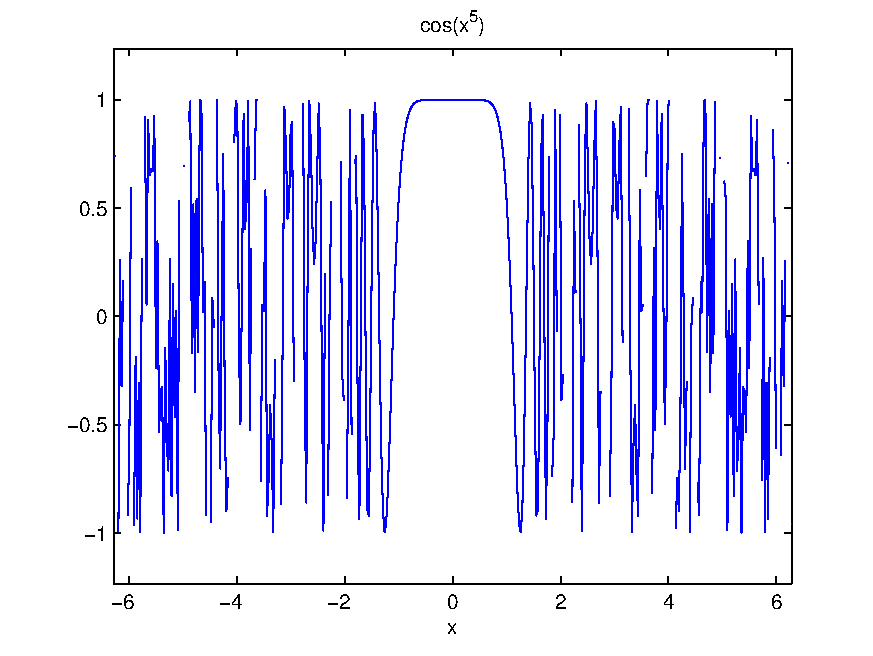
\psfig{figure=cosx5.eps,height=3in,width=3.2in}}}
%\centerline{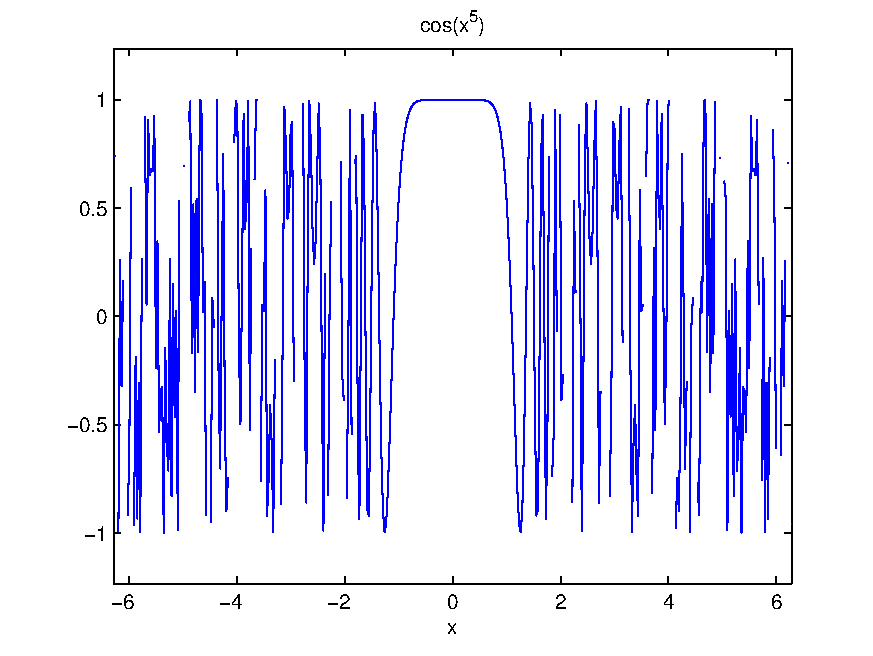
\includegraphics[width=0.6\textwidth]{cosx5}}
%\caption{Graph of $\cos(x^5)$ produced by the ezplot
%command. It is wrong because $\cos u$ should oscillate smoothly between
%$-1$ and $1$. The problem with the plot is that $\cos(x^5)$ oscillates
%extremely rapidly, and the plot did not consider enough points.}
%\label{fig:cosx5}
%\end{figure}
%
%%%%%%%%%%%%%%%%

\newpage

\subsection*{Functions of Two Variables and Partial Derivatives}

Since $f = \cos(x) + 3x^2$ and $g = \exp(-y^2)$ are functions of different variables,
their product is a function of two variables:
$$
k(x,y) = f(x) g(y) = ( \cos(x) + 3 x^2) \exp(-y^2)
$$
In \textsc{Matlab}, set
\begin{lstlisting}[frame=none,numbers=left]
k = f*g
\end{lstlisting}
To evaluate, we need to specify which value goes in which variable:
\begin{lstlisting}[frame=none,numbers=left]
subs(k,[x,y],[0,1])
\end{lstlisting}
To plot a symbolic function of two variables use:
\begin{lstlisting}[frame=none,numbers=left]
ezsurf(k)
\end{lstlisting}


If we want to differentiate a function with more than one variable in \textsc{Matlab}, we
must specify which variable we are differentiating with respect to:
\begin{lstlisting}[frame=none,numbers=left]
k1x = diff(k,x)
\end{lstlisting}
Here we have differentiated with respect to $x$. This is called the {\bf partial derivative} with respect to $x$ and
we use the symbol ${\displaystyle \frac{\partial k}{\partial x}}$ to denote it.
There is also a partial derivative with respect to $y$, i.e.\ ${\displaystyle \frac{\partial k}{\partial y}}$:
\begin{lstlisting}[frame=none,numbers=left]
k1y = diff(k,y)
\end{lstlisting}


To calculate a partial derivative by hand you differentiate as normal with respect to one variable, but
treat the other variables as if they were constants. For example if  $f(x,y) = x y^2$, then 
 $$
 \frac{\partial f}{ \partial x} = y^2 \quad \text{ and } \quad \frac{\partial f}{ \partial y} = 2 xy.
$$

\subsection*{Other useful symbolic operations}

\textsc{Matlab} allows you to do simple algebra. For instance:
\begin{lstlisting}[frame=none,numbers=left]
poly = (x - 3)^5
polyex = expand(poly)
polysi = simplify(polyex)
\end{lstlisting}
To find the symbolic solutions of an equation, $f(x) = 0$,
use:
\begin{lstlisting}[frame=none,numbers=left]
solve(f)
solve(g)
solve(polyex)
\end{lstlisting}
Another useful property of symbolic functions is that
you can substitute numerical vectors for the variables:
\begin{lstlisting}[frame=none,numbers=left]
X = 2:0.1:4;
Y = subs(polyex,X);
plot(X,Y)
\end{lstlisting}

\subsection*{New Notation}

\textsc{Matlab} recently expanded it notation for symbolic computations:
\begin{lstlisting}[frame=none,numbers=left]
syms x
f(x) = x^2;
f(2)
\end{lstlisting}
The function must be given as $f(x)$. If given as $f = x^2$ this will not work. Then we have to use 
\begin{lstlisting}[frame=none,numbers=left]
subs(f,2)
\end{lstlisting}
It works for multivariable functions also:
\begin{lstlisting}[frame=none,numbers=left]
syms x y a b
f(x,y) = x + 2*y;
f(a,b)
\end{lstlisting}

%%%%%%%%%%%%%%%%
\newpage
\subsection*{Exercises}
\begin{list}
{\arabic{chapter}.\arabic{exercise}}{\usecounter{exercise}}

\item Starting from \verb&mynewton& write a well-commented {\bf
    function} program \verb&mysymnewton& that takes as its input a
  symbolic function $f$ and the ordinary variables $x_0$ and $n$.  Let
  the program take the symbolic derivative $f'$. You will need to use the command
  \verb&subs& to obtain values of $f(x)$ and $f'(x)$. Test it on $f(x)=x^3-4$
  starting with $x_0=2$.  Turn in the program and a brief summary of
  the results.
  
  
\item Find a {\em complicated} function in an engineering or science
  textbook or website.  Make a well-commented {\bf script} program that defines 
  a symbolic version of this function and takes its derivative and
  indefinite integral symbolically (if possible). Plot the function on the domain that is relevant
  for the application. In the comments of the script
  describe what the function is and properly reference where you got
  it. Turn in your script and the plot.


\item Calculate all the partial derivative for the functions below. 
Do them by hand, then check them using the symbolic toolbox.

\hspace*{1cm} (a)  ${\displaystyle f(x,y) = \sqrt{xy} + x^2 \sin^2{y} }$   \qquad  \qquad  (b)  ${\displaystyle g(u,v) = \frac{uv}{u+v}}$.

\end{list}


%%%%%%%%%%%%%%%%%%%%%%%%%%%%%%%%%%%%%%%%%%%%%%%%%%%%%%%%%%%%%%%%%%%%%%

\chapter*{Review of Part I}
\addcontentsline{toc}{chapter}{Review of Part I}
\markboth{REVIEW OF PART I}{}



%%%%%%%%%%%%%%%%

\subsection*{Methods and Formulas}

%%%%%%%%%%%%%%%%

\subsubsection*{Solving equations numerically:}
\begin{description}
\item[$f(x) = 0$] --- an equation we wish to solve.
\item[$x^*$] --- a true solution.
\item[$x_0$] --- starting approximation.
\item[$x_n$] --- approximation after $n$ steps.
\item[$e_n = x_n - x^*$] --- error of $n$-th step.
\item[$r_n = y_n = f(x_n)$] --- residual at step $n$. 
Often $|r_n|$ is sufficient.
\end{description}

%%%%%%%%%%%%%%%%

\subsubsection*{Newton's method:}
\begin{equation*}
x_{i+1} = x_i - \frac{f(x_i)}{f'(x_i)}
\end{equation*}

%%%%%%%%%%%%%%%%

\subsubsection*{Bisection method:}
$f(a)$ and $f(b)$ must have different signs.\\
$x = (a+b)/2$\\
Choose $a = x$ or $b = x$, depending on signs.\\
$x^*$ is always inside $[a,b]$.\\
$e < (b-a)/2$, current maximum error.

%%%%%%%%%%%%%%%%

\subsubsection*{Secant method:}
\begin{equation*}
x_{i+1} = x_i - \frac{x_i - x_{i-1}}{y_i - y_{i-1}} y_i
\end{equation*}

%%%%%%%%%%%%%%%%

\subsubsection*{Regula Falsi} - a hybrid between secant and bisection methods.
\begin{equation*}
x = b - \frac{b - a}{f(b) - f(a)} f(b)
\end{equation*}
Choose $a = x$ or $b = x$, depending on signs.

%%%%%%%%%%%%%%%%

\subsubsection*{Convergence:}
Bisection is very slow.\\
Newton is very fast.\\
Secant methods are intermediate in speed.\\
Bisection and Regula Falsi never fail to converge.\\
Newton and Secant can fail if $x_0$ is not close to $x^*$.

%%%%%%%%%%%%%%%%

\subsubsection*{Locating roots:}
Use knowledge of the problem to begin with a reasonable domain.\\
Systematically search for sign changes of $f(x)$.\\
Choose $x_0$ between sign changes using bisection or secant.


%%%%%%%%%%%%%%%%

\subsubsection*{Usage:}
For Newton's method one must have formulas for $f(x)$ and $f'(x)$.\\
Secant methods are better for experiments and simulations.\\
Bisection and {\em Regula Falsi} are slower, but keep the root within the current bounds.

%%%%%%%%%%%%%%%%

\subsection*{\textsc{Matlab}}


%%%%%%%%%%%%%%%%

\subsubsection*{Commands:}

% \begin{lstlisting}[frame=none,numbers=left]
% v = [0 1 2 3]          % Make a row vector
% u = [0; 1; 2; 3]       % Make a column vector
% w = v'                 % Transpose: row vector --> column vector
% x = linspace(0,1,11)   % Make an evenly spaced vector of length 11
% x = -1:.1:1            % Make an evenly spaced vector, with increments 0.1
% y = x.^2               % Square all entries
% plot(x,y)              % plot y vs. x
% f = @(x) 2*x.^2 - 3*x + 1   % Make a function
% y = f(x)               % A function can act on a vector
% plot(x,y,'*','red')    % A plot with options
% Control-c              % Stops a computation.
% \end{lstlisting}

\verb&v = [0 1 2 3]& \dotfill Make a row vector.\\
\verb&u = [0; 1; 2; 3]& \dotfill Make a column vector.\\
\verb&w = v'& \dotfill Transpose: row vector $\leftrightarrow$ column vector \\
\verb&x = linspace(0,1,11)& \dotfill Make an evenly spaced vector of
                               length 11.\\
\verb&x = -1:.1:1& \dotfill Make an evenly spaced vector, with increments
                               $0.1$.\\
\verb&y = x.^2&  \dotfill Square all entries.\\
\verb&plot(x,y) & \dotfill plot y vs. x.\\
\verb&f = @(x) 2*x.^2 - 3*x + 1 & \dotfill Make an anonymous function.\\
\verb&y = f(x) &  \dotfill A function can act on a vector.\\
\verb&plot(x,y,'*','red')& \dotfill A plot with options.\\
\verb&Control-c & \dotfill Stops a computation.
%%%%%%%%%%%%%%%%

\subsubsection*{Program structures:}
\verb&for ... end& example:
\begin{lstlisting}
for i=1:20
   S = S + i;
end
\end{lstlisting}
\verb&if  ... end& example:
\begin{lstlisting}
if y == 0
    disp('An exact solution has been found')
end
\end{lstlisting}
\verb&while  ...  end& example:
\begin{lstlisting}
while i <= 20
   S = S + i;
   i = i + 1;
end
\end{lstlisting}
\verb&if  ... else ... end& example:
\begin{lstlisting}
if c*y>0
    a = x;
else
    b = x;
end
\end{lstlisting}

%%%%%%%%%%%%%%%%

\subsubsection*{Function Programs:}
\begin{itemize}
\item Begin with the word \verb&function&.
\item There are inputs and outputs.
\item The outputs, name of the function and the inputs must appear in the first line.\\
\hspace*{.5cm} i.e. \verb&function x = mynewton(f,x0,n)&
\item The body of the program must assign values to the outputs.
\item Internal variables are not visible outside the function.
\item A function program may not use variables in the current
                  workspace unless they are inputs.
\end{itemize}

%%%%%%%%%%%%%%%%

\subsubsection*{Script Programs:}
\begin{itemize}
\item There are no inputs and outputs.
\item A script program may use, create, change and even delete variables in the current
  workspace.
\end{itemize}

%%%%%%%%%%%%%%%%

\subsubsection*{Symbolic:}

% \begin{lstlisting}[frame=none,numbers=left]
% syms x y
% f = 2*x^2 - sqrt(3*x)
% subs(f,sym(pi))
% double(ans)
% g = log(abs(y))   % log is the natural logarithm
% h(x) = compose(g,f)
% k(x,y) = f*g
% ezplot(f)
% ezplot(g,-10,10)
% ezsurf(k)
% f1 = diff(f,x)
% F = int(f,x)      % indefinite integral (antiderivative)
% int(f,0,2*pi)     % definite integral
% poly = x*(x - 3)*(x-2)*(x-1)*(x+1)
% polyex = expand(poly)
% polysi = simple(polyex)
% solve(f)
% solve(g)
% solve(polyex)
% \end{lstlisting}
\verb&syms x y&\\
\verb&f = 2*x^2 - sqrt(3*x)&\\
\verb&subs(f,sym(pi)) &\\
\verb&double(ans)&\\
\verb&g = log(abs(y))& \dotfill \textsc{Matlab} uses \verb&log& for
                                     natural logarithm.\\
\verb&h(x) = compose(g,f)&\\
\verb&k(x,y) = f*g &\\
\verb&fplot(f)&\\
\verb&fplot(g,-10,10)&\\
\verb&ezsurf(k)&\\
%
\verb&f1 = diff(f,'x')& \\
\verb&F = int(f,'x')& \dotfill indefinite integral (antiderivative)\\
\verb&int(f,0,2*pi)& \dotfill definite integral\\
%
\verb&poly = x*(x - 3)*(x-2)*(x-1)*(x+1)&\\
\verb&polyex = expand(poly)&\\
\verb&polysi = simple(polyex)&\\
%
\verb&solve(f)&\\
\verb&solve(g)&\\
\verb&solve(polyex)&


%%%%%%%%%%%%%%%%%%%%%%%%%%%%%%%%%%%%%%%%%%%%%%%%%%%%%%%%%%%%%
%%%%%%%%%%%%%%%%%%%%%%%%%%%%%%%%%%%%%%%%%%%%%%%%%%%%%%%%%%%%%
%%%%%%%%%%%%%%%%%%%%%%%%%%%%%%%%%%%%%%%%%%%%%%%%%%%%%%%%%%%%%
\part{Linear Algebra}

%%%%%%%%%%%%%%%%%%%%%%%%%%%%%%%%%%%%%%%%%%%%%%%%%%%%%%%

\chapter{Matrices and Matrix Operations in Matlab}

%%%%%%%%%%%%%%%%

You should review the vector operations in Lecture~\ref{lec:vectors}.

\subsection*{Matrix operations}

Recall how to multiply a matrix $A$ times a vector $\vb$:
$$
   A \vb = \left( \begin{array}{cc}
                    1 & 2  \\
                    3 & 4  \\
                   \end{array} \right)
                    \left( \begin{array}{c}
                    -1  \\
                    2 \\
                   \end{array} \right)
=
\left( \begin{array}{c}
                    1 \cdot (-1) + 2 \cdot 2  \\
                    3 \cdot (-1) + 4 \cdot 2 \\
                   \end{array} \right)
=
\left( \begin{array}{c}
                   3  \\
                   5 \\
                   \end{array} \right).
$$
This is a special case of matrix multiplication. To
multiply two matrices, $A$ and $B$ you proceed as follows:
$$
   A B = \left( \begin{array}{cc}
                    1 & 2  \\
                    3 & 4  \\
                   \end{array} \right)
\left( \begin{array}{cc}
                    -1 & -2 \\
                    2 &  1\\
                   \end{array} \right)
=
\left( \begin{array}{cc}
                    -1 + 4 & -2 + 2  \\
                    -3 + 8 & -6 + 4 \\
                   \end{array} \right)
=
\left( \begin{array}{cc}
                   3 & 0 \\
                   5 & -2 \\
                   \end{array} \right).
$$
Here both $A$ and $B$ are $2 \times 2$ matrices.
Matrices can be multiplied together in this way provided
that the number of columns of $A$ match the number of rows
of $B$. We always list the size of a matrix by rows, then
columns, so a $3 \times 5$ matrix would have 3 rows and 5 columns.
So, if $A$ is $m \times n$ and $B$ is $p \times q$, then
we can multiply $AB$ if and only if $n = p$.
A column vector can be thought of as a $p \times 1$ matrix
and a row vector as a $1 \times q$ matrix. Unless otherwise specified
we will assume a vector $\vb$ to be a column vector and
so $A\vb $ makes sense as long as the number of columns of $A$
matches the number of entries in $\vb$.

Printing matrices on the screen takes up a lot of space, so you may
want to use
\begin{lstlisting}[frame=none,numbers=left]
format compact
\end{lstlisting}
Enter a matrix into Matlab either as
\begin{lstlisting}[frame=none,numbers=left]
A = [ 1  3 -2 5 ;  -1  -1 5 4 ; 0 1 -9  0]
\end{lstlisting}
or
\begin{lstlisting}[frame=none,numbers=left]
A = [1,3,-2,5; -1,-1,5,4; 0,1,-9,0]
\end{lstlisting}
Also enter a vector $\ub$:
\begin{lstlisting}[frame=none,numbers=left]
u = [ 1  2  3  4]'
\end{lstlisting}
To multiply a matrix times a vector $A\mathbf{u}$ use \verb&*&:
\begin{lstlisting}[frame=none,numbers=left]
A*u
\end{lstlisting}
Since $A$ is 3 by 4 and $\ub$ is 4 by 1 this multiplication is
valid and the result is a 3 by 1 vector.

Now enter another matrix $B$ using
\begin{lstlisting}[frame=none,numbers=left]
B = [3 2 1; 7 6 5; 4 3 2]
\end{lstlisting}
You can multiply $B$ times $A$ with
\begin{lstlisting}[frame=none,numbers=left]
B*A
\end{lstlisting}
but $A$ times $B$ is not defined and
\begin{lstlisting}[frame=none,numbers=left]
A*B
\end{lstlisting}
will result in an error message.


You can multiply a matrix by a scalar:
\begin{lstlisting}[frame=none,numbers=left]
2*A
\end{lstlisting}
Adding matrices $A + A$ will give the same result:
\begin{lstlisting}[frame=none,numbers=left]
A + A
\end{lstlisting}
You can even add a number to  a matrix:
\begin{lstlisting}[frame=none,numbers=left]
A + 3    % add 3 to every entry of A
\end{lstlisting}

%%%%%%%%%%%%%%%%

\subsection*{Component-wise operations}

Just as for vectors, adding a `\verb&.&' before `\verb&*&',
`\verb&/&', or `\verb&^&' produces entry-wise multiplication,
division and exponentiation.
If you enter
\begin{lstlisting}[frame=none,numbers=left]
B*B
\end{lstlisting}
the result will be $BB$, i.e.\ matrix multiplication of $B$ times itself. But,
if you enter
\begin{lstlisting}[frame=none,numbers=left]
B.*B
\end{lstlisting}
the entries of the resulting matrix will contain the squares
of the same entries of $B$. Similarly if you want $B$  multiplied
by itself 3 times then enter
\begin{lstlisting}[frame=none,numbers=left]
B^3
\end{lstlisting}
but, if you want to cube all the entries of B then enter
\begin{lstlisting}[frame=none,numbers=left]
B.^3
\end{lstlisting}
Note that \verb&B*B& and \verb&B^3& only make sense if $B$ is
square, but \verb&B.*B& and \verb&B.^3& make sense for any size
matrix.


%%%%%%%%%%%%%%%%

\subsection*{The identity matrix and the inverse
of a matrix}

The $n \times n$ {\em identity matrix} is a square matrix with
ones on the diagonal and zeros everywhere else. It is
called the identity because it plays the same role that $1$
plays in multiplication, i.e.
$$
      A I = A,   \qquad I A = A, \qquad I \vb = \vb
$$
for any matrix $A$ or vector $\vb$ where the sizes match.
An identity matrix in \textsc{Matlab} is produced by the command
\begin{lstlisting}[frame=none,numbers=left]
I = eye(3)
\end{lstlisting}

A square matrix $A$ can have an {\em inverse} which is denoted
by $A^{-1}$. The definition of the inverse is that
$$
       A A^{-1} = I  \qquad \text{and} \qquad A^{-1} A = I.
$$
In theory an inverse is very important, because if you
have an equation
$$
     A \xb = \bb
$$
where $A$ and $\bb$ are known and $\xb$ is unknown (as
we will see, such problems are very common and important)
then the theoretical solution is
$$
      \xb = A^{-1} \bb.
$$
We will see later that this is not a practical way to solve
an equation, and $A^{-1}$ is only important for the purpose
of derivations.
%
In \textsc{Matlab} we can calculate a matrix's inverse
very conveniently:
\begin{lstlisting}[frame=none,numbers=left]
C = randn(5,5)
inv(C)
\end{lstlisting}
%
However, not all square matrices have inverses:
\begin{lstlisting}[frame=none,numbers=left]
D = ones(5,5)
inv(D)
\end{lstlisting}


%%%%%%%%%%%%%%%%


\subsection*{The ``Norm'' of a matrix}

For a vector, the ``norm'' means the same thing as the length (geometrically, not the number of entries).
Another way to think of it is how far the vector is from being
the zero vector.
We want to measure a matrix in much the same way and the {\em
norm} is such a quantity. The usual definition of the norm of
a matrix is
\begin{defn}
Suppose $A$ is a $m \times n$ matrix. The norm of $A$ is
$$
  \|A\| \equiv  \max_{\|\vb\|=1} \|A\vb\|.
$$
\end{defn}
The maximum in the definition is taken over all vectors with
length $1$ (unit vectors), so the definition means the largest
factor that the matrix stretches (or shrinks) a unit vector.
This definition seems cumbersome at first, but it
turns out to be the best one. For example, with this definition
we have the following inequality for any vector $\vb$:
$$
    \|A\vb\| \le \|A\| \|\vb\|.
$$
In \textsc{Matlab} the norm of a matrix is obtained by the
command
\begin{lstlisting}[frame=none,numbers=left]
norm(A)
\end{lstlisting}
For instance the norm of an identity matrix is $1$:
\begin{lstlisting}[frame=none,numbers=left]
norm(eye(100))
\end{lstlisting}
and the norm of a zero matrix is $0$:
\begin{lstlisting}[frame=none,numbers=left]
norm(zeros(50,50))
\end{lstlisting}

For a matrix the norm defined above and calculated by
\textsc{Matlab} is not the square root of the sum
of the square of its entries. That quantity is called the
{\em Froebenius norm}, which is also sometimes useful,
but we will not need it.

%%%%%%%%%%%%%%%%%

\subsection*{Some other useful commands}

% Try out the following:
% \begin{lstlisting}[frame=none,numbers=left]
% C = rand(5,5)    % random matrix with uniform distribution in [0,1]
% size(C)          % gives the dimensions (m x n) of C
% det(C)           % the determinant of the matrix
% max(C)           % the maximum of each column
% min(C)           % the minimum in each column
% sum(C)           % sums each column
% mean(C)          % the average of each column
% diag(C)          % just the diagonal elements
% C'               % tranpose the matrix
% \end{lstlisting}
\verb&C = rand(5,5)& \dotfill random matrix with uniform
         distribution in $[0,1]$.\\
\verb&size(C)& \dotfill gives the dimensions ($m\times n$) of $C$.\\
\verb&det(C)&   \dotfill the determinant of the matrix.\\
\verb&max(C)&   \dotfill the maximum of each column.\\
\verb&min(C)&   \dotfill the minimum in each column.\\
\verb&sum(C)&   \dotfill sums each column.\\
\verb&mean(C)&   \dotfill the average of each column.\\
\verb&diag(C)&   \dotfill just the diagonal elements.\\
\verb&C'&   \dotfill tranpose the matrix.

In addition to \verb&ones&, \verb&eye&, \verb&zeros&, \verb&rand& and
\verb&randn&,  \textsc{Matlab} has several other commands that
automatically produce special matrices:
%\begin{lstlisting}[frame=none,numbers=left]
%hilb(6)
%pascal(5)
%\end{lstlisting}
\\
\verb&hilb(6)&\\
\verb&pascal(5)&


%%%%%%%%%%%%
\newpage
\subsection*{Exercises}
\begin{list}
{\arabic{chapter}.\arabic{exercise}}{\usecounter{exercise}}


\item Enter the matrix $A$ by
\begin{lstlisting}[frame=none,numbers=left]
A = [3 2 1; 6 5 4; 9 8 7]
\end{lstlisting}
and also the matrix
$$
B = \left[
{\begin{array}{rrr}
7 & 8 & 9 \\
4 & 5 & 6 \\
1 & 2 & 3 
\end{array}}
\right]\,.  $$
Find  (a) \verb&A*A&, (b) \verb&A^2&, (c) \verb&A.^2&, (d) \verb&A.*B&, (e) \verb&A*B&. Turn in the output.

\item By hand, calculate $A \vb$, $AB$, and $BA$ for:
      $$
        A = \left( \begin{array}{ccc}
                    2 & 4 & -1 \\
                    -2 & 1 & 9 \\
                    -1 & -1 & 0 \\
                   \end{array} \right),
        \quad
        B = \left( \begin{array}{ccc}
                    0 & -1 & -1 \\
                    1 & 0 & 2 \\
                    -1 & -2 & 0 \\
                   \end{array} \right),
        \quad
        \vb = \left( \begin{array}{c}
                    3  \\
                    1  \\
                    -1 \\
                   \end{array} \right).
     $$
     Check the results using \textsc{Matlab}. Think about how
     fast computers are. Turn in your hand work.

\item  Write a well-commented \textsc{Matlab} {\bf function} program
    \verb&myinvcheck& that
    \begin{itemize}
    \item makes a $n \times n$ random matrix (normally distributed,
      \verb&A = randn(n,n)&),
    \item calculates its inverse (\verb&B = inv(A)&),
    \item multiplies the two back together,
    \item calculates the residual (difference between $AB$ and \verb&eye(n)&), and
    \item returns the scalar residual (norm of the difference).
    \end{itemize}
    Turn in your program.
  
 \item Write a well-commented \textsc{Matlab} {\bf script} program \verb&myinvcheckplot& that calls
    \verb&myinvcheck& for $n=10,20,40,\ldots,2^i10$ for $i$ as large as possible, 
    records the
    results of each trial, and plots the scalar residual versus \verb&n& 
    using a log plot. (See \verb&help loglog&.)
 
   What happens to the scalar residual as \(n\)
  gets big? Turn in the program, the plot, and a very brief report on
  the results of your experiments.  (Do not print any large random matrices.) 

\end{list}


%%%%%%%%%%%%%%%%%%%%%%%%%%%%%%%%%%%%%%%%%%

\chapter{Introduction to Linear Systems}
\label{chp:intro_linsys}
%%%%%%%%%%%%%%%%

\subsection*{How linear systems occur}


Linear systems of equations naturally occur in many places
in engineering, such as structural analysis, dynamics and
electric circuits. Computers have made it possible to
quickly and accurately solve larger and larger systems
of equations. Not only has this allowed engineers to handle
more and more complex problems where linear systems naturally
occur, but has also prompted engineers to use linear systems
to solve problems where they do not naturally occur such
as thermodynamics, internal stress-strain analysis, fluids and
chemical processes. It has become standard practice in
many areas to analyze a problem by transforming it into a linear
systems of equations and then solving those equation by computer.
In this way, computers have made linear systems of equations
the most frequently used tool in modern engineering.


In Figure~\ref{equilateral_truss} we show a truss with equilateral
triangles. In Statics you may use the ``method of joints'' to write
equations for each node of the truss\footnote{See
  http://en.wikipedia.org/wiki/Truss or
  http://en.wikibooks.org/wiki/Statics for reference.}.  This set of
equations is an example of a linear system.  Making the approximation
$\sqrt{3}/2 \approx .8660$, the equations for this truss are
\begin{equation}
\label{truss_equilateral_eqns}
\begin{split}
  .5 \, T_1 + T_2 & = R_1 = f_1 \\
  .866 \, T_1 & = - R_2 = -.433 \, f_1 - .5 \, f_2 \\
  -.5 \, T_1 + .5 \, T_3 + T_4 &= - f_1 \\
  .866 \, T_1 + .866 \, T_3 &= 0 \\
  -T_2 - .5 \, T_3 + .5 \, T_5 + T_6 &= 0 \\
  .866 \, T_3 + .866 \, T_5 &= f_2 \\
  -T_4 - .5 \, T_5 + .5 \, T_7 &=0, \\
\end{split}
\end{equation}
where $T_i$ represents the tension in the $i$-th member of the truss.
%
% \begin{figure}
% \setlength{\unitlength}{1 mm}
% \LARGE
% \begin{center}
% \begin{picture}(64,17)(0,-1)
% 	\put(0,0){\line(1,0){64}}
% 	\put(16,16){\line(1,0){32}}
% 	\put(0,0){\line(1,1){16}}
% 	\put(16,0){\line(1,1){16}}
% 	\put(64,0){\line(-1,1){16}}
% 	\put(48,0){\line(-1,1){16}}
% 	\put(16,0){\line(0,1){16}}
% 	\put(48,0){\line(0,1){16}}
% 	\put(0,0){\circle*{2}}
% 	\put(16,0){\circle*{1}}
% 	\put(48,0){\circle*{1}}
% 	\put(64,0){\circle*{2}}
% 	\put(16,16){\circle*{1}}
% 	\put(32,16){\circle*{1}}
% 	\put(48,16){\circle*{1}}
% \end{picture}
% \end{center}
% \caption{A truss.}
% \label{truss}
% \end{figure}



\begin{figure}[ht]
\setlength{\unitlength}{1 mm}
% \LARGE
 \begin{center}
 \begin{picture}(64,40)(0,-10)
% nodes
 	\put(0,0){\circle*{2}}
 	\put(32,0){\circle*{1}}
 	\put(64,0){\circle*{2}}
 	\put(16,27.7){\circle*{1}}
 	\put(48,27.7){\circle*{1}}
	\put(3,1){A}
	\put(14,21){B}
	\put(31,4){C}
	\put(47,22){D}
	\put(59,1){E}
% edges
 	\put(0,0){\line(1,0){64}}
 	\put(16,27.7){\line(1,0){32}}
	\qbezier(0,0)(8,13.85)(16,27.7)
	\qbezier(32,0)(40,13.85)(48,27.7)
	\qbezier(16,27.7)(24,13.85)(32,0)
	\qbezier(48,27.7)(56,13.85)(64,0)
	\put(4,12){1}
	\put(15,1){2}
	\put(26,12){3}
	\put(31,24){4}
	\put(41,12){5}
	\put(47,1){6}
	\put(57,13){7}
% forces
 	\put(6,27.7){\vector(1,0){6}}
	\put(2,27){$f_1$}
 	\put(32,-1){\vector(0,-1){6}}
	\put(31,-10){$f_2$}
 	\put(0,-7){\vector(0,1){5}}
	\put(-1,-10){$R_2$}
 	\put(64,-7){\vector(0,1){5}}
	\put(62,-10){$R_3$}
 	\put(-2,0){\vector(-1,0){6}}
	\put(-13,-1){$R_1$}
% 	\put(16,0){\line(1,1){16}}
% 	\put(64,0){\line(-1,1){16}}
% 	\put(48,0){\line(-1,1){16}}
% 	\put(16,0){\line(0,1){16}}
% 	\put(48,0){\line(0,1){16}}
 \end{picture}
\end{center}
%\centerline{\hbox{\psfig{figure=equilateral_truss3.eps,height=1.5in,width=2.5in}}}
\caption{An equilateral truss. Joints or nodes are labeled alphabetically, $A$, $B$, \ldots
and Members (edges) are labeled numerically: $1$, $2$, \ldots. The forces $f_1$ and $f_2$
are applied loads and $R_1$, $R_2$ and $R_3$ are reaction forces applied by the supports.}
\label{equilateral_truss}
\end{figure}



You could solve
this system by hand with a little time and patience; systematically
eliminating variables and substituting.
Obviously, it would be a lot better to put the equations
on a computer and let the computer solve it. In the next few lectures
we will learn how to use a computer effectively to solve linear systems.
The first key to dealing with linear systems is to realize that
they are equivalent to matrices, which contain numbers, not variables.

As we discuss various aspects of matrices, we wish to keep in
mind that the matrices that come up in engineering systems are
{\em really  large}. It is not unusual in real engineering
to use matrices whose dimensions are in the thousands!
It is frequently the case that a method that is fine for
a $2 \times 2$ or $3 \times 3$ matrix is totally inappropriate
for a $2000 \times 2000$ matrix. We thus want to emphasize methods
that work for large matrices.


%%%%%%%%%%%%%%%

\subsection*{Linear systems are equivalent to matrix equations}
\label{lec:LSME}

The system of linear equations
\begin{equation*}
\begin{split}
     x_1 - 2 x_2 + 3 x_3 & = 4 \\
     2 x_1 - 5x_2 + 12 x_3 & = 15 \\
           2 x_2 -  10 x_3 & = -10 
\end{split}
\end{equation*}
is equivalent to the matrix equation
$$
\left(\begin{array}{ccc}
        1 & -2 & 3  \\
        2 & -5 & 12 \\
        0 & 2 & -10
      \end{array}\right)
\left(\begin{array}{c}
       x_1 \\ x_2 \\ x_3
      \end{array} \right)
=
\left(\begin{array}{c}
       4\\ 15 \\ -10
      \end{array} \right),
$$
which is equivalent to the {\em augmented matrix}
$$
\left(\begin{array}{ccc|c}
        1 & -2 & 3 & 4 \\
        2 & -5 & 12 & 15 \\
        0 & 2 & -10 & -10
      \end{array}\right).
$$
The advantage of the augmented matrix, is that it contains only
numbers, not variables. The reason this is better is because computers
are much better in dealing with numbers than variables. To solve
this system, the main steps are called {\em Gaussian elimination} and
{\em back substitution}.

The augmented matrix for the equilateral truss equations
(\ref{truss_equilateral_eqns}) is given by
\begin{equation}\label{truss_equilateral_matrix}
\left(\begin{array}{ccccccc|c}
        .5    & 1 & 0 & 0 & 0 & 0 & 0 & f_1 \\
        .866  & 0 & 0  & 0 & 0 & 0 &  0 & -.433  f_1 - .5 \, f_2  \\
         -.5  & 0 & .5 &  1 & 0 & 0 & 0  & - f_1 \\
        .866  & 0 & .866  & 0 & 0 & 0 & 0 & 0 \\
         0    & -1 & - .5  & 0 & .5 & 1 &  0 & 0 \\
         0    & 0  & .866  & 0 & .866 & 0 & 0 &  f_2 \\
         0 &  0 &  0  & -1  & - .5  &0 & .5 & 0 \\
      \end{array}\right).
\end{equation}
Notice that a lot of the entries are $0$. Matrices like this, called
{\em sparse}, are common in applications and there are methods
specifically designed to efficiently handle sparse matrices.


%%%%%%%%%%%%%%%%

\subsection*{Triangular matrices and back substitution}

Consider a linear system whose augmented matrix happens to be
\begin{equation}\label{upper}
\left(\begin{array}{ccc|c}
        1 & -2 & 3 & 4 \\
        0 & -1 & 6 & 7 \\
        0 & 0 & 2 & 4
      \end{array}\right).
\end{equation}
Recall that each row represents an equation and each column a variable.
The last row represents the equation $2 x_3 = 4$. The equation is
easily solved, i.e. $x_3 = 2$. The second row represents the equation
$- x_2 + 6 x_3 = 7$, but since we know $x_3 = 2$, this simplifies to:
$ - x_2 + 12 = 7$. This is easily solved, giving $x_2 = 5$. Finally,
since we know $x_2$ and $x_3$, the first row simplifies to:
$x_1 - 10 + 6 = 4$. Thus we have $x_1 = 8$ and so we know the
whole solution vector: $\xb = \langle 8 , 5, 2 \rangle$. The process
we just did is called {\em back substitution}, which is both efficient
and easily programmed. The property that made it possible
to solve the system so easily is that $A$ in this case is {\em upper
triangular}. In the next section we show an efficient way to
transform an augmented matrix into an upper triangular matrix.


%%%%%%%%%%%%%%%%

\subsection*{Gaussian Elimination}

Consider the matrix
$$
 A = \left(\begin{array}{ccc|c}
        1 & -2 & 3  &  4 \\
        2 & -5 & 12 & 15 \\
        0 & 2 & -10 & -10
      \end{array}\right).
$$
The first step of Gaussian elimination is to get rid of the 2 in
the (2,1) position by subtracting $2$ times the first row
from the second row, i.e. {\sf (new 2nd = old 2nd - (2) 1st)}.
We can do this because it is essentially the
same as adding equations, which is a valid
algebraic operation.  This leads to
$$
\left(\begin{array}{ccc|c}
        1 & -2 & 3 & 4 \\
        0 & -1 & 6 & 7 \\
        0 & 2 & -10 & -10
      \end{array}\right).
$$
There is already a zero in the lower left corner, so we don't need to
eliminate anything there. To eliminate the third row, second column,
we need to subtract $-2$ times the second row from the third row, {\sf
  (new 3rd = old 3rd - (-2) 2nd)}, to obtain
$$
\left(\begin{array}{ccc|c}
        1 & -2 & 3 &  4 \\
        0 & -1 & 6 &  7 \\
        0 &  0 & 2 &  4
      \end{array}\right).
$$
This is now just exactly the matrix in equation (\ref{upper}), which
we can now solve by back substitution.


%%%%%%%%%%%%%%%%

\subsection*{\textsc{Matlab}'s matrix solve command}

In \textsc{Matlab} the standard way to solve a system $A \xb = \bb$
is by the command
\begin{lstlisting}[frame=none,numbers=left]
x = A \ b
\end{lstlisting}
This syntax is meant to suggest dividing by \(A\) from the left as in
\[A \xb = \bb \quad \Leftrightarrow\quad A\backslash A \xb = A\backslash \bb 
\quad \Leftrightarrow\quad  \xb = A\backslash \bb
\,.\]
Such division is not meaningful mathematically, but it helps for remembering the syntax.

This command carries out Gaussian elimination and back substitution.
We can do the above computations as follows:
\begin{lstlisting}[frame=none,numbers=left]
A = [1 -2 3 ; 2 -5 12 ; 0 2 -10]
b = [4 15 -10]'
x = A \ b
\end{lstlisting}

Next, use the \textsc{Matlab} commands above to solve $A \xb = \bb$ when
the augmented matrix for the system is
 $$
\left(\begin{array}{ccc|c}
        1 & 2 & 3 &  4 \\
        5 & 6 & 7 &  8 \\
        9 &  10 & 11 &  12
      \end{array}\right),
$$
by entering
\begin{lstlisting}[frame=none,numbers=left]
x1 = A \ b
\end{lstlisting}
Check the result by entering
\begin{lstlisting}[frame=none,numbers=left]
A*x1 - b
\end{lstlisting}
You will see that the resulting answer satisfies the equation exactly.
Next try solving using the inverse of $A$:
\begin{lstlisting}[frame=none,numbers=left]
x2 = inv(A)*b
\end{lstlisting}
This answer can be seen to be inaccurate by checking
\begin{lstlisting}[frame=none,numbers=left]
A*x2 - b
\end{lstlisting}
Thus we see one of the reasons why the inverse is never used for actual
computations, only for theory.

%%%%%%%%%%%%%%%%

\subsection*{Exercises}
\nobreak
\begin{list}
{\arabic{chapter}.\arabic{exercise}}{\usecounter{exercise}}

\item  Set $f_1 = 1000N$ and $f_2 = 5000N$ in
the equations (\ref{truss_equilateral_eqns}) for the equailateral truss.
Input the coefficient matrix $A$ and the right hand side vector $b$ in
(\ref{truss_equilateral_matrix}) into \textsc{Matlab}.
Solve the system using the command \verb&\& to find the tension in each member of the
truss. Save the matrix $A$ as \verb&A_equil_truss& and keep it for later use.
(Enter \verb& save A_equil_truss A&.)
Print out and turn in $A$, $\bb$ and the solution $\xb$.
\label{exr:truss}

\item Write each system of equations as an augmented matrix. By hand, find
the solutions using {\em Gaussian elimination and back substitution} (i.e.\ the exact
algorithm in this chapter). Check
your solutions using \textsc{Matlab}.

\begin{enumerate}[(a)]
\item 
\begin{equation*}
\begin{split}
     x_1 +  x_2   & = 2 \\
   4 x_1 + 5 x_2  & = 10
\end{split}
\end{equation*}
\item
\begin{equation*}
\begin{split}
     x_1 + 2 x_2 + 3 x_3 & = -1 \\
   4 x_1 + 7 x_2 + 14 x_3 & = 3 \\
    x_1 +  4 x_2 + 4 x_3 & =  1
\end{split}
\end{equation*}
\end{enumerate}

\end{list}



%%%%%%%%%%%%%%%%%%%%%%%%%%%%%%%%%%%%%%%%%%%

\chapter{Some Facts About Linear Systems}
\label{sec:lineartheory}


%%%%%%%%%%%%%%%%

\subsection*{Some inconvenient truths}


In the last lecture we learned how to solve a linear system
using \text{Matlab}.
Input the following:
\begin{lstlisting}[frame=none,numbers=left]
A = ones(4,4)
b = randn(4,1)
x = A \ b
\end{lstlisting}

As you will find, there is no solution to the equation $A \xb = \bb$.
This unfortunate circumstance is mostly the fault of the matrix, $A$,
which is too simple, its columns (and rows) are all the same.
Now try
\begin{lstlisting}[frame=none,numbers=left]
b = ones(4,1)
x = [ 1 0 0 0]'
A*x
\end{lstlisting}
So the system $A \xb = \bb$ does have a solution. Still unfortunately,
that is not the only solution. Try
\begin{lstlisting}[frame=none,numbers=left]
x = [ 0 1 0 0]'
A*x
\end{lstlisting}
We see that this $x$ is also a solution. Next try
\begin{lstlisting}[frame=none,numbers=left]
x = [ -4  5  2.27 -2.27]'
A*x
\end{lstlisting}
This $x$ is a solution! It is not hard to see that
there are endless possibilities for solutions of this
equation.

%%%%%%%%%%%%%%%

\subsection*{Basic theory}


The most basic theoretical fact about linear systems is
\begin{thm}
A linear system $A\xb = \bb$ may have 0, 1, or infinitely many solutions.
\end{thm}
In most (but not all!) engineering applications we would want to
have exactly one solution. The following two theorems tell us
exactly when we can and cannot expect this.
\begin{thm}
Suppose $A$ is a square ($n \times n $) matrix.
The following are all equivalent:
\begin{enumerate}
\item The equation $A\xb = \bb$ has exactly one solution for any $\bb$.
\item $det(A) \ne 0$.
\item $A$ has an inverse.
\item The only solution of $A\xb = \mathbf{0}$ is $\xb = \mathbf{0}$.
\item The columns of $A$ are linearly independent (as vectors).
\item The rows of $A$ are linearly independent.
\end{enumerate}
If $A$ has these properties then it is called {\bf non-singular}.
\end{thm}

On the other hand, a matrix that does not have these properties
is called {\bf singular}.
\begin{thm}\label{def:singular}
Suppose $A$ is a square  matrix.
The following are all equivalent:
\begin{enumerate}
\item The equation $A\xb = \bb$ has 0 or $\infty$ many solutions
  depending on $\bb$.
\item $\det(A) = 0$.
\item $A$ does not have an inverse.
\item The equation $A\xb = \mathbf{0}$ has solutions other than $\xb =
  \mathbf{0}$.
\item The columns of $A$ are linearly dependent as vectors.
\item The rows of $A$ are linearly dependent.
\end{enumerate}
\end{thm}


To see how the two theorems work, define two matrices (type in
\verb&A1& then scroll
up and modify to make \verb&A2&) :
$$
\verb&A1& = \left(\begin{array}{ccc}
        1 & 2 & 3  \\
        4 & 5 & 6 \\
        7 & 8 & 9
      \end{array}\right),
\qquad
\verb&A2& = \left(\begin{array}{ccc}
        1 & 2 & 3  \\
        4 & 5 & 6 \\
        7 & 8 & 8
      \end{array}\right),
$$
and two vectors:
$$
\verb&b1&  = \left(\begin{array}{c}
        0 \\ 3 \\ 6
             \end{array}\right),
\qquad
\verb&b2&  = \left(\begin{array}{c}
        1 \\ 3 \\ 6
             \end{array}\right).
$$
First calculate the determinants of the matrices:
\begin{lstlisting}[frame=none,numbers=left]
det(A1)
det(A2)
\end{lstlisting}
Then attempt to find the inverses:
\begin{lstlisting}[frame=none,numbers=left]
inv(A1)
inv(A2)
\end{lstlisting}
Which matrix is singular and which is non-singular?
Finally, attempt to solve all the possible equations $A \xb = \bb$:
\begin{lstlisting}[frame=none,numbers=left]
x = A1 \ b1
x = A1 \ b2
x = A2 \ b1
x = A2 \ b2
\end{lstlisting}
As you can see, equations involving the non-singular matrix have one
and only one solution, but equation involving a singular matrix
are more complicated.

%%%%%%%%%%%%%%%%

\subsection*{The Residual}

Recall that the residual for an approximate solution $x$
of an equation $f(x) =0$ is defined as $r = \|f(x)\|$.
It is a measure of how close the equation is to being satisfied.
For a linear system of equations we define the residual vector
of an approximate solution $\xb$ by
\begin{equation*}
%\label{lsres}
\rb = A \xb - \bb.
\end{equation*}
If the solution vector $\xb$ were exactly correct, then $\rb$ would be 
exactly the zero vector.  The size (norm)  of $\rb$ is
an indication of how close we have come to solving
$A \xb = \bb$. We will refer to this number as the {\bf scalar residual} or just  the {\bf residual} of the
approximation solution:
\begin{equation}
   r = \| A \xb - \bb \|.
\end{equation}


%%%%%%%%%%%%%%%

\subsection*{Exercises}
\nobreak
\begin{list}
  {\arabic{chapter}.\arabic{exercise}}{\usecounter{exercise}}


\item By hand, find all the solutions (if any) of the following linear
  system using the augmented matrix and Gaussian elimination (following exactly
  the algorithm in the notes):
  \begin{equation*}
    \begin{split}
      x_1 + 2 x_2 + 3 x_3 & = 4, \\
      4 x_1 + 5 x_2 + 6 x_3 & = 10, \\
      7 x_1 + 8 x_2 + 9 x_3 & = 14 \,.
    \end{split}
  \end{equation*}
Try solving this system in \textsc{Matlab} using the command \verb&x = A \ b&. What happens?
Turn in your hand work.

\item
  \begin{enumerate}
  \item[(a)] Write a well-commented \textsc{Matlab} {\bf function}
    program \verb&mysolvecheck& with input a number \verb&n& that
    makes a random $n \times n$ matrix $A$ and a random vector $\bb$,
    solves the linear system $A \xb = \bb$, calculates the scalar
    residual $r = \|A \xb - \bb\|$, and outputs that number as  $r$.
  \item[(b)] Write a well-commented \textsc{Matlab} {\bf script}
    program that calls \verb&mysolvecheck& 10 times each for $n = $
    5, 10, 20, 40, 80, and 160, then records and averages the
    results and makes a log-log plot of the average $r$ vs.\ $n$. 
    Once your program is running correctly, increase the maximum $n$ (by factors of $2$) until the program stops running 
    within 5 minutes.
  \end{enumerate}
  Turn in the plot and the two programs. (Do not print any large random matrices.)
\end{list}


%%%%%%%%%%%%%%%%%%%%%%%%%%%%%%%%%%%%%%%%%%%%%%%%

\chapter{Accuracy, Condition Numbers and Pivoting}

In this lecture we will discuss two separate issues
of accuracy in solving linear systems. The first,
{\em pivoting}, is a method that ensures that Gaussian
elimination proceeds as accurately as possible.
The second, {\em condition number}, is a measure
of how bad a matrix is. We will see that if a matrix has
a bad condition number, the solutions are unstable with
respect to small changes in data.

%%%%%%%%%%%%%

\subsection*{The effect of rounding}

All computers store numbers as  finite strings of binary
floating point digits (bits). This limits numbers to a fixed
number of significant digits and implies that after even
the most basic calculations, rounding must happen.

Consider the following exaggerated example. Suppose
that our computer can only store 2 significant digits
and it is asked to do Gaussian elimination on
\begin{equation*}
\left(\begin{array}{cc|c}
        .001 & 1 & 3  \\
          1 &  2 & 5
      \end{array}\right).
\end{equation*}
Doing the elimination exactly would produce
\begin{equation*}
\left(\begin{array}{cc|c}
        .001 & 1 & 3  \\
          0 & -998 & -2995
      \end{array}\right),
\end{equation*}
but rounding to 2 digits, our computer would store this as
\begin{equation*}
\left(\begin{array}{cc|c}
        .001 & 1 & 3  \\
          0 &  -1000 & -3000
      \end{array}\right).
\end{equation*}
Backsolving this reduced system gives
$$
     x_1 = 0 \quad\text{and}\quad x_2 = 3.
$$
This seems fine until you realize that backsolving the unrounded
system gives
$$
    x_1 = -1 \quad\text{and}\quad x_2 = 3.001.
$$

%%%%%%%%%%%%%%%

\subsection*{Row Pivoting}


A way to fix the problem is to use pivoting, which means to switch rows of
the matrix. Since switching rows of the augmented matrix
just corresponds to switching the order of the equations, no harm
is done:
\begin{equation*}
\left(\begin{array}{cc|c}
          1 &  2 & 5  \\
        .001 & 1 & 3
      \end{array}\right).
\end{equation*}
Exact elimination would produce
\begin{equation*}
\left(\begin{array}{cc|c}
          1 &  2 & 5  \\
          0 & .998 & 2.995
      \end{array}\right).
\end{equation*}
Storing this result with only 2 significant digits gives
\begin{equation*}
\left(\begin{array}{cc|c}
          1 &  2 & 5  \\
          0 & 1 & 3
      \end{array}\right).
\end{equation*}
Now backsolving produces
$$
      x_1 = -1 \quad\text{and}\quad x_2 = 3,
$$
which is the true solution (rounded to 2 significant digits).

The reason this worked is because $1$ is bigger than $0.001$. To pivot
we switch rows so that the largest entry in a column is the one used
to eliminate the others. In bigger matrices, after each column is completed,
compare the diagonal element of the next column with all the entries below
it. Switch it (and the entire row) with the one with greatest absolute value.
For example in the following matrix, the first column is finished and before
doing the second column, pivoting should occur since $|-2|>|1|$:
$$
\left(\begin{array}{ccc|c}
        1 & -2 & 3 & 4 \\
        0 &  1 & 6 & 7 \\
        0 & -2 & -10 & -10
      \end{array}\right).
$$
Pivoting the 2nd and 3rd rows would produce
$$
\left(\begin{array}{ccc|c}
        1 & -2 & 3 & 4 \\
        0 & -2 & -10 & -10\\
        0 &  1 & 6 & 7
      \end{array}\right).
$$

%%%%%%%%%%

\subsection*{Condition number}

In some systems, problems occur even without rounding.
Consider the following augmented matrices:
$$
\left(\begin{array}{cc|c}
        1   & 1/2 & 3/2  \\
        1/2 & 1/3 &  1  \\
      \end{array}\right)
     \quad \text{and} \quad
\left(\begin{array}{cc|c}
        1   & 1/2  & 3/2 \\
        1/2 & 1/3  & 5/6\\
      \end{array}\right).
$$
Here we have the same $A$, but two different input vectors:
$$  \bb_1 = (3/2,1)' \quad \textrm{and} \quad \bb_2 = (3/2,5/6)'
$$
which are pretty close to one another. You would
expect then that the solutions $\xb_1$ and $\xb_2$ would also be close.
Notice that this matrix does not need pivoting. Eliminating exactly
we get
$$
\left(\begin{array}{cc|c}
        1 & 1/2  & 3/2  \\
        0 & 1/12 & 1/4 \\
      \end{array}\right)
     \quad \text{and} \quad
\left(\begin{array}{cc|c}
        1 & 1/2  & 3/2 \\
        0 & 1/12 & 1/12\\
      \end{array}\right).
$$
Now solving we find
$$
   \xb_1 = (0,3)' \quad \textrm{and} \quad \xb_2 = (1,1)'
$$
which are {\em not close at all} despite the fact that we did the
calculations exactly. This poses a new problem: some matrices
are very sensitive to small changes in input data. The extent of
this sensitivity is measured by the {\bf condition number}.
The definition of condition number is: consider all small changes
$\delta A$ and $\delta \bb$ in $A$ and $\bb$  and the resulting
change, $\delta \xb$, in the solution $\xb$. Then
$$
      \textrm{cond}(A) \equiv \max \left( \frac{ \|\delta \xb\|/\|\xb\|}
         { \frac{\|\delta A\|}{\|A\|} + \frac{\|\delta \bb\|}{\|\bb\|} } \right) =
     \max \left( \frac{\text{Relative error of output}}
                      {\text{Relative error of inputs}} \right).
$$
Put another way, changes in the input data get multiplied by the condition number
to produce changes in the outputs.
Thus a high condition number is bad. It implies that small errors
in the input can cause large errors  in the output.
%
It is not obvious from our definition above, but one can prove that the condition number of a matrix is at least 1.


In \textsc{Matlab} enter
\begin{lstlisting}[frame=none,numbers=left]
H = hilb(2)
\end{lstlisting}
which should result in the matrix above. \textsc{Matlab} produces the
condition number of a matrix with the command
\begin{lstlisting}[frame=none,numbers=left]
cond(H)
\end{lstlisting}
Thus for this matrix small errors in the input can get magnified
by 19 in the output.
Next try the matrix
\begin{lstlisting}[frame=none,numbers=left]
A = [ 1.2969 0.8648 ; .2161  .1441]
cond(A)
\end{lstlisting}
For this matrix small errors in the input can get magnified
by $2.5 \times 10^8$ in the output! (We will see this happen in the exercise.)
This is obviously not very good for engineering
where all measurements, constants and inputs are approximate.

Is there a solution to the problem of bad condition numbers?
Usually, bad condition numbers in engineering contexts result
from poor design. So, the engineering solution to bad conditioning
is {\bf redesign}.

Finally, find the determinant of the matrix $A$ above:
\begin{lstlisting}[frame=none,numbers=left]
det(A)
\end{lstlisting}
which will be small. If $\det(A) = 0$ then the matrix is singular,
which is bad because it implies there will not be a unique solution.
The case here, $\det(A) \approx 0$, is also bad, because it means the
matrix is almost singular. Although $\det(A) \approx 0$ generally
indicates that the condition number will be large, they are actually
independent things. To see this, find the determinant and condition
number of the matrix \verb&[1e-10,0;0,1e-10]& and
the matrix \verb&[1e+10,0;0,1e-10]&.

%%%%%%%%%%%%%%%%%%%%%%%%
\newpage

\subsection*{Exercises}
\begin{list}
{\arabic{chapter}.\arabic{exercise}}{\usecounter{exercise}}

%%%
\item Let $$
A = \left[
{\begin{array}{cc}
1.2969 & .8648 \\
.2161 & .1441
\end{array}}
 \right]\,.
$$
\begin{enumerate}
\item[(a)] Find the condition number, determinant and inverse of $A$ (using \textsc{Matlab}).
\item[(b)] Let $B$ be the matrix obtained from $A$ by rounding off to three
  decimal places ($1.2969\mapsto 1.297$).  Find the inverse of $B$.  
  How do $A^{-1}$ and $B^{-1}$ differ? Explain how
  this happened.
\item[(c)] Set \verb&b1 = [1.2969; 0.2161] & and do \verb&x = A \ b1 &.
  Repeat the process but with a vector \verb&b2& obtained from
  \verb&b1& by rounding off to three decimal places. Explain exactly
  what happened.  Why was the first answer so simple?  Why do the two
  answers differ by so much?
\end{enumerate}

%%%%%%%%%%
\item To see how to solve linear systems symbolically, try
\begin{lstlisting}[frame=none,numbers=left]
B = [sin(sym(1)) sin(sym(2)); sin(sym(3)) sin(sym(4))]
c = [1; 2]
x = B \ c
pretty(x)
\end{lstlisting}

Now input the matrix
\[
\textsf{Cs = }\left[
\begin{array}{rr}
1 & 2 \\
2 & 4
\end{array}
\right]
\]
symbolically as above by wrapping each number in \verb&sym&. Create a numerical version via
\verb&Cn = double(Cs)& and define the two vectors \verb$ d1 = [4; 8] $ and
\verb$ d2 = [1; 1]$.
Solve the systems (as in the third line of code above) \verb&Cs*x = d1&, \verb&Cn*x = d1&,
\verb&Cs*x = d2&, and \verb&Cn*x = d2&.
Explain the results.  Does the symbolic or
non-symbolic way give more information?
%
%\item Recall the matrix $A$ that you saved using \verb&A_equil_truss&
%  in exercise \ref{lec:LSME}.\ref{exr:truss}.  (Enter
%  \verb&> load A_equil_truss& or click on the file
%  \verb&A_equil_truss.mat& in the folder where you saved it; this
%  should reproduce the matrix $A$.)

%  Find the condition number and determinant of this matrix.  
  
%  Write a well-commented
%  {\bf script} program to calculate the mean and median condition
%  number of 1000 randomly generated 7 by 7 matrices.  How does the
%  condition number of the truss matrix compare to randomly generated
%  matrices? Turn in your script with the answers to these questions.

%\textsf{The matrix in 1.\ is nearly singular, causing the linear system to be
%very sensitive to perturbations.  Students are exposed to both
%symbolic and numerical solutions.  The ideas of no solutions or
%infinitely many solutions are reinforced.}

\end{list}

%%%%%%%%%%%%%%%%%%%%%%%%%%%%%%%%%%%%%%%%%%%%%%%%%%%%%%%%%%%%%%

\chapter{LU Decomposition}

In many applications where linear systems appear, one needs to solve
$A \xb = \bb$ for many different vectors $\bb$. For instance, a
structure must be tested under several different loads, not just one.
As in the example of a truss (\ref{truss_equilateral_matrix}),
the loading in such a problem is usually
represented by the vector $\bb$.  Gaussian elimination with pivoting
is the most efficient and accurate way to solve a linear system.  Most
of the work in this method is spent on the matrix $A$ itself.  If we
need to solve several different systems with the same $A$, and $A$ is
big, then we would like to avoid repeating the steps of Gaussian
elimination on $A$ for every different $\bb$. This can be accomplished
by the {\em LU decomposition}, which in effect records the steps of
Gaussian elimination.

%%%%%%%%%%%%%%%%

\subsection*{LU decomposition}

The main idea of the LU decomposition
is to record the steps used in Gaussian elimination on A
in the places where the zero is produced.
Consider the matrix
$$
 A = \left(\begin{array}{ccc}
        1 & -2 & 3 \\
        2 & -5 & 12  \\
        0 & 2 & -10
      \end{array}\right).
$$
The first step of Gaussian elimination is to subtract $2$ times the
first row from the second row. In order to record what we have done,
we will put the multiplier, $2$, into the place it was used to make a
zero, i.e. the second row, first column. In order to make it clear
that it is a record of the step and not an element of $A$, we will put
it in parentheses. This leads to
$$
\left(\begin{array}{ccc}
        1 & -2 & 3 \\
        (2) & -1 & 6  \\
        0 & 2 & -10
      \end{array}\right).
$$
There is already a zero in the lower left corner, so we don't need to eliminate
anything there. We record this fact with a $(0)$. To eliminate the third row,
second column, we need to subtract
$-2$ times the second row from the third row. Recording the $-2$ in the spot
it was used we have
$$
\left(\begin{array}{ccc}
        1 & -2 & 3 \\
        (2) & -1 & 6  \\
        (0) & (-2) & 2
      \end{array}\right).
$$
Let $U$ be the upper triangular matrix produced, and let $L$ be the lower
triangular matrix with the records and ones on the diagonal, i.e.
$$
L = \left(\begin{array}{ccc}
        1 & 0 & 0 \\
        2 & 1 & 0  \\
        0 & -2 & 1
      \end{array}\right)
\quad\text{and}\quad
U = \left(\begin{array}{ccc}
         1 & -2 & 3 \\
         0 & -1 & 6  \\
         0 &  0 & 2
      \end{array}\right),
$$
then we have the following wonderful property:
$$
  LU = \left(\begin{array}{ccc}
        1 & 0 & 0 \\
        2 & 1 & 0  \\
        0 & -2 & 1
      \end{array}\right)
      \left(\begin{array}{ccc}
        1 & -2 & 3 \\
        0 & -1 & 6  \\
        0 & 0 & 2
      \end{array}\right)
=   \left(\begin{array}{ccc}
        1 & -2 & 3 \\
        2 & -5 & 12  \\
        0 & 2 & -10
      \end{array}\right)
= A.
$$
Thus we see that $A$ is actually the product of $L$ and $U$.
Here $L$ is lower triangular and $U$ is upper triangular.
When a matrix can be written as a product of simpler
matrices, we call that a {\em decomposition} of $A$ and
this one we call the LU decomposition.

%%%%%%%%%%%%%%%%%%

\subsection*{Using LU to solve equations}

If we also include pivoting, then an LU decomposition for $A$
consists of three matrices $P$, $L$ and $U$ such that
\begin{equation}\label{LUP}
   PA = LU.
\end{equation}
The pivot matrix $P$ is the identity matrix, with the same rows switched
as the rows of $A$ are switched in the pivoting. For instance,
$$
P = \left(\begin{array}{ccc}
        1 & 0 & 0 \\
        0 & 0 & 1  \\
        0 & 1 & 0
      \end{array}\right),
$$
would be the pivot matrix if the second and third rows of $A$ are
switched by pivoting.  \textsc{Matlab} will produce an $LU$
decomposition with pivoting for a matrix $A$
with the command\\
\verb& > [L U P] = lu(A)&\\
where \verb&P& is the pivot matrix. To use this information to solve
$A \xb = \bb$ we first pivot both sides by multiplying by the pivot
matrix:
$$
     PA \xb = P \bb \equiv \mathbf{d}.
$$
Substituting $LU$ for $PA$ we get
$$
     LU \xb = \mathbf{d} .
$$
Then we define $\yb=U \xb$, which is unknown since \(\xb\) is unknown. 
Using forward-substitution, we can (easily) solve
$$
     L \yb = \mathbf{d}
$$
for \(\yb\) and then using back-substitution we can (easily) solve 
$$
     U \xb = \yb
$$
for \(\xb\).
In \textsc{Matlab} this would work as follows:
\begin{lstlisting}[frame=none,numbers=left]
A = rand(5,5)
[L U P] = lu(A)
b = rand(5,1)
d = P*b
y = L\d
x = U\y
rnorm = norm(A*x - b)  % Check the result
\end{lstlisting}
We can then solve for any other $\bb$ without redoing the LU step.
Repeat the sequence for a new right hand side: \verb&c = randn(5,1)&;
you can start at the third line.
While this may not seem like a big savings, it would be if $A$ were a large
matrix from an actual application.


The LU decomposition is an example of {\em Matrix Decomposition} which
means taking a general matrix $A$ and breaking it down into components
with simpler properties.  Here $L$ and $U$ are simpler because they
are lower and upper triangular. There are many other matrix
decompositions that are useful in various contexts. Some of the most
useful of these are the QR decomposition, the Singular Value
decomposition and Cholesky decomposition. Often a decomposition
is associated with an algorithm, e.g., finding the LU decomposition is equivalent
to completing Gaussian Elimination.


%%%%%%%%%%%%%%

\subsection*{Exercises}
\begin{list}
{\arabic{chapter}.\arabic{exercise}}{\usecounter{exercise}}

\item Solve the systems below by hand using Gaussian elimination  and
back substitution (exactly as above) on the augmented matrix. 
As a by-product, give the LU decomposition
of A. Pivot wherever appropriate (the number being eliminated should be smaller than the 
number eliminating it). Check by hand that
$LU=PA$ and $A\xb = \bb$ and compare with \textsc{Matlab}.
\begin{enumerate}
\item[(a)] $\displaystyle{ A =
      \left(\begin{array}{cc} 0.5 & 4 \\
                               2 & 4
           \end{array} \right), \qquad \bb = \left(\begin{array}{c} 0 \\
                                                                -3 \end{array} \right)}
$
\item[(b)] $\displaystyle{ A =
      \left(\begin{array}{ccc} 1 & 2 & 3 \\
                             4 & 1 & 1 \\
                             2 & 3 & 9
           \end{array} \right), \qquad \bb = \left(\begin{array}{c} 2 \\
                                                                                                1 \\
                                                                                                1  \end{array} \right)}
$
\end{enumerate}


\item
Finish the following \textsc{Matlab} function program:
\begin{lstlisting}
function [x1, r1, x2, r2] = mysolve(A,b)
    % Solves linear systems using the LU decomposition with pivoting
    % and also with the built-in solve function A\b.
    % Inputs: A -- the matrix
    %         b -- the right-hand vector
    % Outputs: x1 -- the solution using the LU method
    %          r1 -- the scalar residual using the LU method
    %          x2 -- the solution using the built-in method
    %          r2 -- the scalar residual using the 
    %                built-in method
\end{lstlisting}

Using \verb&format long&, test the program on both random matrices
(\verb&randn(n,n)&) and Hilbert matrices (\verb&hilb(n)&) with $n$
large (as big as you can make it and the program still run). Print
your program and summarize your observations.  (Do not print any
random matrices or vectors.)
\end{list}


%%%%%%%%%%%%%%%%%%%%%%%%%%%%%%%%%%%%%%%%%%%%%%%%%

\chapter{Nonlinear Systems - Newton's Method}
\label{lec:multnewton}

%%%%%%%%%%%%%%%%

\subsection*{An Example}

The LORAN (LOng RAnge Navigation) system calculates the position
of a boat at sea using signals from fixed transmitters. From
the time differences of the incoming signals, the boat obtains
differences of distances to the transmitters. This leads
to two equations each representing hyperbolas defined
by the differences of distance of two points (foci). An example
of such equations\footnote{E.~Johnston, J.~Mathews, {\em Calculus}, Addison-Wesley, 2001} are
\begin{equation}\label{eqn:loran}
\begin{split}
   \frac{x^2}{186^2} - \frac{y^2}{300^2 - 186^2} &= 1
\quad\text{and}\\
  \frac{(y-500)^2}{279^2} - \frac{(x-300)^2}{500^2 - 279^2} &= 1
\,.
\end{split}
\end{equation}


Solving two quadratic equations with two unknowns would require
solving a 4 degree polynomial equation. We could do this by hand, but
for a navigational system to work well, it must do the calculations
automatically and numerically. We note that the Global Positioning
System (GPS) works on similar principles and must do similar
computations.

%%%%%%%%%%%%

\subsection*{Vector Notation}

In general, we can usually find solutions to a system of equations
when the number of unknowns matches the number of equations.
Thus, we wish to find solutions to systems that have the form
\begin{equation}\label{nlsys}
\begin{split}
f_1(x_1, x_2, x_3, \ldots , x_n) & = 0 \\
f_2(x_1, x_2, x_3, \ldots , x_n) & = 0 \\
f_3(x_1, x_2, x_3, \ldots , x_n) & = 0 \\
      \vdots \hspace*{1.4cm}      &  \\
f_n(x_1, x_2, x_3, \ldots , x_n) & = 0. \\
\end{split}
\end{equation}

For convenience we can think of $(x_1, x_2, x_3, \ldots , x_n)$ as
a vector $\xb$ and $(f_1, f_2, \ldots, f_n)$ as a vector-valued function
$\fb$. With this notation, we can write the system of equations (\ref{nlsys})
simply as
$$
   \fb(\xb) = \mathbf{0},
$$
i.e.\ we wish to find a vector that makes the vector function equal to
the zero vector.

As in Newton's method for one variable, we need to start with an
initial guess $\xb_0$. In theory, the more variables one has, the
harder it is to find a good initial guess. In practice, this must
be overcome by using physically reasonable assumptions about
the possible values of a solution, i.e.~take advantage of engineering
knowledge of the problem.

%%%%%%%%%%%%

\subsection*{Linear Approximation for Vector Functions}

In the single variable case, Newton's method was derived
by considering the linear approximation of the function $f$ at
the initial guess $\xb_0$.
From Calculus, the following is the linear approximation of
$\fb$ at $\xb_0$, for vectors and vector-valued functions:
$$
\fb(\xb) \approx \fb(\xb_0) + D\fb(\xb_0) (\xb - \xb_0).
$$
Here $D\fb(\xb_0)$ is an $n \times n$ matrix whose entries are the
various partial derivative of the components of $\fb$, evaluated at
\(\xb_0\). Specifically,
\begin{equation}
  \label{eq:Df}
   D\fb(\xb_0) = \left( \begin{array}{ccccc}
     \frac{\partial f_1}{\partial x_1}(\xb_0) & \frac{\partial f_1}{\partial x_2}(\xb_0) &
              \frac{\partial f_1}{\partial x_3}(\xb_0) & \ldots & \frac{\partial f_1}{\partial x_n}(\xb_0) \vspace*{.3cm} \\

     \frac{\partial f_2}{\partial x_1}(\xb_0) & \frac{\partial f_2}{\partial x_2}(\xb_0) &
              \frac{\partial f_2}{\partial x_3}(\xb_0) & \ldots & \frac{\partial f_2}{\partial x_n}(\xb_0) \vspace*{.15cm}\\
        \vdots & \vdots  & \vdots & \ddots & \vdots \vspace*{.15cm}\\
     \frac{\partial f_n}{\partial x_1}(\xb_0) & \frac{\partial f_n}{\partial x_2}(\xb_0) &
              \frac{\partial f_n}{\partial x_3}(\xb_0) & \ldots & \frac{\partial f_n}{\partial x_n}(\xb_0)
                       \end{array} \right).  
\end{equation}

%%%%%%%%%%%%

\subsection*{Newton's Method}

We wish to find $\xb$ that makes $\fb$ equal to the zero vectors, so
let's choose $\xb_1$ so that
$$
  \fb(\xb_0) + D\fb(\xb_0) (\xb_1 -\xb_0) = \mathbf{0}.
$$
Since $D\fb(\xb_0)$ is a square matrix, we can solve this equation
by
$$
\xb_1 = \xb_0 - (D\fb(\xb_0))^{-1} \fb(\xb_0),
$$
provided that the inverse exists. The formula is the vector equivalent
of the Newton's method formula we learned before.
However, in practice we never use the inverse of a matrix for
computations, so we cannot use this formula directly. Rather,
we can do the following. First solve the equation
\begin{equation}
D\fb(\xb_0) \Delta \xb = -\fb(\xb_0)\,,
\end{equation}
where we want to have
$$
\Delta \xb = \xb_1 - \xb_0.
$$
Since $D\fb(\xb_0)$ is a known matrix and $-\fb(\xb_0)$ is a known
vector, this equation is just a system of linear equations,
which can be solved efficiently and accurately. Once we have the
solution vector $\Delta \xb$, we can obtain our improved estimate
$\xb_1$ by
$$
   \xb_1 = \xb_0 + \Delta \xb.
$$

For subsequent steps, we have the following process:
\begin{itemize}
\item Solve $D\fb(\xb_i) \Delta \xb = -\fb(\xb_i)$ for $\Delta \xb$.
\item Let $\xb_{i+1} = \xb_i + \Delta \xb$
\end{itemize}

%%%%%%%%%%%%%%

\subsection*{An Experiment}

We will solve the following set of equations:
\begin{equation}
\begin{split}
x^3 + y &= 1 \\
y^3 - x & = -1.
\end{split}
\end{equation}
You can easily check that $(x,y) = (1,0)$ is a solution of this system.
By graphing both of the equations you can also see that $(1,0)$ is the
only solution (Figure~\ref{fig:nlsys}).
\begin{figure}
\centerline{
\includegraphics[width=0.6\textwidth]{nlsys}}
\caption{Graphs of the equations $x^3 + y = 1$ and  $y^3 - x  = -1$.
There is one and only one intersection; at $(x,y) = (1,0)$.}
\label{fig:nlsys}
\end{figure}

We can put these equations into vector-function form (\ref{nlsys})
by letting $x_1 = x$,
$x_2 = y$ and
\begin{equation*}
\begin{split}
f_1(x_1,x_2) &= x_1^3 + x_2 - 1 \\
f_2(x_1,x_2) &= x_2^3 - x_1 + 1\,,
\end{split}
\end{equation*}
or, equivalently,
\begin{equation*}
\fb(\xb) = \left(\begin{array}{c}
                   x_1^3 + x_2 - 1 \\
                   x_2^3 - x_1 + 1
                  \end{array} \right).
\end{equation*}
The partial derivatives are
\begin{equation}
\label{eqn:partials}
\frac{\partial f_1}{\partial x_1} = 3 x_1^2, 
\quad \frac{\partial f_1}{\partial x_2} = 1, 
\quad \frac{\partial f_2}{\partial x_1} = -1,  
\quad\text{and}\quad \frac{\partial f_2}{\partial x_2} = 3 x_2^2.
\end{equation}
Thus,
\begin{equation}
\label{eqn:Dfexample}
D \mathbf{f} =  \left(\begin{array}{cc}
                   3x_1^2 & 1 \\
                    -1 & 3x_2^2 
                  \end{array} \right).
\end{equation}
Now that we have the equations in  vector-function form,
we can write the following script program:
\begin{lstlisting}
format long;
f = @(x)[ x(1)^3+x(2)-1 ; x(2)^3-x(1)+1 ]
x = [.5;.5]
x = fsolve(f,x)
\end{lstlisting}
Save this program as \verb&myfsolve.m& and run it.
You will see that the internal \textsc{Matlab} solving
command \verb&fsolve& approximates the solution, but
only to about 7 decimal places. While that would be close enough
for most applications, one would expect that we could do
better on such a simple problem.

Next we will implement Newton's method for this problem.
Modify your \verb&myfsolve& program to:
\begin{lstlisting}
% mymultnewton - solve an example nonlinear system
format long;
n=8  % set some number of iterations, may need adjusting
f = @(x)[x(1)^3+x(2)-1 ; x(2)^3-x(1)+1] % the vector function
% the matrix of partial derivatives
Df = @(x)[3*x(1)^2,  1 ; -1,  3*x(2)^2] 
x = [.5;.5]             % starting guess
for i = 1:n
      Dx = -Df(x)\f(x); % solve for increment
      x = x + Dx        % add on to get new guess
      f(x)              % see if f(x) is really zero
end
\end{lstlisting}

Save and run this program (as \verb&mymultnewton&) and you will see that it
finds the root exactly (to machine precision)
in only 6 iterations. Why is this simple program able to do better
than \textsc{Matlab}'s built-in program?

%%%%%%%%%%%

\subsection*{Exercises}
\begin{list}
{\arabic{chapter}.\arabic{exercise}}{\usecounter{exercise}}

\item 
  \begin{enumerate}[(a)]
  \item Put the LORAN equations (\ref{eqn:loran}) into the
    function form (\ref{nlsys}).
  \item  Calculate (by hand) the partial derivatives of $\mathbf{f}$
  and construct the matrix $D\fb$  (see (\ref{eqn:partials}) and (\ref{eqn:Dfexample})).
  \item Adapt the \verb&mymultnewton& program to find a solution
    for these equations.  By trying different starting vectors, find
    at least three different solutions. (There are actually four
    solutions.)  
   \item Think of at least one way that the navigational
    system could determine the correct solution.
  \end{enumerate}

\end{list}







%%%%%%%%%%%%%%%%%%%%%%%%%%%%%%%%%%%%%%%%%%%%%%%%%

\chapter{Eigenvalues and Eigenvectors}

Suppose that $A$ is a square ($n \times n$) matrix.
We say that a  nonzero vector $\vb$ is an eigenvector
and a number $\lambda$ is its eigenvalue if
\begin{equation}\label{def:eig}
   A \vb = \lambda \vb.
\end{equation}

Geometrically this means that $A\vb$ is in the same direction
as $\vb$, since multiplying a vector by a number changes
its length, but not its direction.\\

\textsc{Matlab} has a built-in routine for finding eigenvalues and eigenvectors:
\begin{lstlisting}[frame=none,numbers=left]
A = pascal(4)
[v e] = eig(A)
\end{lstlisting}
The results are a matrix \verb&v& that contains eigenvectors as
columns and a diagonal matrix \verb&e& that contains eigenvalues on
the diagonal. We can check this by
\begin{lstlisting}[frame=none,numbers=left]
v1 = v(:,1)
A*v1
e(1,1)*v1
\end{lstlisting}

%%%%%%%%%%%%%%%%

\subsection*{Finding Eigenvalues for $2\times 2$ and $3\times3$}


If $A$ is $2\times 2$ or $3\times3$ then we can find its eigenvalues
and eigenvectors by hand. Notice that Equation (\ref{def:eig})
can be rewritten as
\begin{equation*}
     A \vb - \lambda \vb = \mathbf{0}.
\end{equation*}
It would be nice to factor out the $\vb$ from the right-hand side of this
equation, but we can't because $A$ is a matrix and $\lambda$ is a number.
However, since $I \vb = \vb$, we can do the following:
\begin{equation*}
\begin{split}
A\vb - \lambda \vb &=    A \vb - \lambda I \vb \\
                   &= (A  - \lambda I) \vb \\
                   &= \mathbf{0}
\end{split}
\end{equation*}
If $\vb$ is nonzero, then by Theorem~\ref{def:singular} in
Lecture~\ref{sec:lineartheory} the matrix $(A - \lambda I)$ must be
singular. By the same theorem, we must have
\begin{equation*}%\label{charac}
         \det(A - \lambda I) = 0.
\end{equation*}
This is called the {\em characteristic equation}.

For a $2 \times 2$ matrix, $A - \lambda I$ is calculated as in the following example:
\begin{equation*}
\begin{split}
 A - \lambda I &=  \left(\begin{array}{cc} 1 & 4 \\
                             3 & 5
                         \end{array} \right)
                  - \lambda  \left(\begin{array}{cc} 1 & 0 \\
                                                    0 & 1
                                   \end{array} \right) \\
               &=  \left(\begin{array}{cc} 1 & 4 \\
                                           3 & 5
                         \end{array} \right)
                  - \left(\begin{array}{cc} \lambda & 0 \\
                                           0 & \lambda
                         \end{array} \right) \\
               &= \left(\begin{array}{cc} 1 -\lambda & 4 \\
                                          3 & 5 - \lambda
                        \end{array} \right)
\,.
\end{split}
\end{equation*}
The determinant of $A - \lambda I$ is then
\begin{equation*}
\begin{split}
\det(A - \lambda I) &= (1 - \lambda)(5 - \lambda) - 4 \cdot 3 \\
                   &= -7 - 6 \lambda + \lambda^2 .
\end{split}
\end{equation*}
The characteristic equation $\det(A - \lambda I) = 0$ is simply a quadratic
equation:
\begin{equation*}
           \lambda^2 - 6 \lambda - 7 = 0.
\end{equation*}
The roots of this equation are $\lambda_1 = 7$ and $\lambda_2 = -1$.
These are the eigenvalues of the matrix $A$. Now to find the corresponding
eigenvectors we return to the equation $(A - \lambda I) \vb = \mathbf{0}$.
For $\lambda_1 = 7$, the equation for the eigenvector
$(A - \lambda I) \vb = \mathbf{0}$ is equivalent
to the augmented matrix
\begin{equation}\label{eveqn}
\left(\begin{array}{cc|c} -6 & 4 & 0\\
                             3 & -2 & 0
                    \end{array} \right) .
\end{equation}
Notice that the first and second rows of this matrix are multiples of
one another. Thus Gaussian elimination would produce all zeros on the bottom row.
Thus this equation has infinitely many solutions, i.e.~infinitely
many eigenvectors. Since only the direction of the eigenvector matters, this is okay,
we only need to find one of the eigenvectors. Since the second row of the augmented
matrix represents the equation
$$
               3 x - 2 y = 0,
$$
we can let
$$
     \vb_1 = \left(\begin{array}{c} 2 \\
                             3
                    \end{array} \right).
$$
This comes from noticing that $(x,y) = (2,3)$ is a solution of
$ 3x -2y =0 $.

For $\lambda_2 = -1$, $(A - \lambda I) \vb = \mathbf{0}$ is equivalent
to the augmented matrix
$$
\left(\begin{array}{cc|c} 2 & 4 & 0\\
                             3 & 6 & 0
                    \end{array} \right)
.
$$
Once again the first and second rows of this matrix are multiples of
one another. For simplicity we can
let
$$
     \vb_2 = \left(\begin{array}{c} -2 \\
                             1
                    \end{array} \right).
$$

One can always check an eigenvector and eigenvalue by multiplying:
\begin{align*}
A \vb_1 &= \left(\begin{array}{cc} 1 & 4 \\
                             3 & 5
                    \end{array} \right)
          \left(\begin{array}{c} 2 \\
                                 3
                    \end{array} \right)
         = \left(\begin{array}{c} 14 \\
                                   21
                    \end{array} \right)
         = 7 \left(\begin{array}{c} 2 \\
                                     3
                    \end{array} \right)
	=7 \vb_1
\quad\text{and}\\
A \vb_2 &= \left(\begin{array}{cc} 1 & 4 \\
                             3 & 5
                    \end{array} \right)
          \left(\begin{array}{c} -2 \\
                                 1
                    \end{array} \right)
         = \left(\begin{array}{c} 2 \\
                                   -1
                    \end{array} \right)
         = -1 \left(\begin{array}{c} -2 \\
                                      1
                    \end{array} \right)
	= -1 \vb_2
\,.
\end{align*}

For a $3 \times 3$ matrix we could complete the same process.
The $\det(A -\lambda I)=0$ would be a cubic polynomial and we
would expect to usually get 3 roots, which are the eigenvalues.


%%%%%%%%%%%%%%%%

\subsection*{Larger Matrices}

For a $n \times n$ matrix with $n \ge 4$ this process is too
long and cumbersome to complete by hand. Further, this process
is not well suited even to implementation on a computer program
since it involves determinants and solving a $n$-degree polynomial.
For $n \ge 4$ we need more ingenious methods. These methods rely
on the geometric meaning of eigenvectors and eigenvalues rather than solving
algebraic equations. We will overview these methods in Lecture~\ref{EWmeth}.



%%%%%%%%%%%%%%%%

\subsection*{Complex Eigenvalues}

It turns out that the eigenvalues of some matrices are complex
numbers, even when the matrix only contains real numbers.
When this happens the complex eigenvalues must occur
in conjugate pairs, i.e.
$$
    \lambda_{1,2} = \alpha \pm i \beta.
$$
The corresponding eigenvectors must also come
in conjugate pairs:
$$
     \wb = \ub \pm i \vb.
$$
In applications, the imaginary part of the eigenvalue, $\beta$,
often is related to the frequency of an oscillation.
This is because of Euler's formula
$$
    e^{\alpha + i \beta} = e^\alpha(\cos \beta + i \sin \beta).
$$

Certain kinds of matrices that arise in applications can only
have real eigenvalues and eigenvectors. The most common such type of matrix
is the symmetric matrix. A matrix is symmetric if it is equal
to its own transpose, i.e.~it is symmetric across the diagonal.
For example,
$$
\left(\begin{array}{cc} 1 & 3 \\
                        3 & -5
                    \end{array} \right)
$$
is symmetric and so we know beforehand that its eigenvalues will be real,
not complex.


%%%%%%%%%%%%%%%%%%%

\subsection*{Exercises}
\begin{list}
{\arabic{chapter}.\arabic{exercise}}{\usecounter{exercise}}

\item Find the eigenvalues and eigenvectors of the following
      matrix by hand:
$$
A = \left(\begin{array}{cc} 2 & 1 \\
                            1 & 2
                    \end{array} \right).
$$


\item Find the eigenvalues and eigenvectors of the following
      matrix by hand:
$$
B = \left(\begin{array}{cc} 1 & -3 \\
                            3 &  1
                    \end{array} \right).
$$
Can you guess the eigenvalues of the matrix
$$
C = \left(\begin{array}{cc} a & -b \\
                            b &  a
                    \end{array} \right)?
$$
\end{list}



%%%%%%%%%%%%%%%%%%%%%%%%%%%%%%%%%%%%%%%%%%%%%%%%%%%%%%%%%%%

\chapter[Vibrational Modes and Frequencies]{An Application of Eigenvectors: Vibrational Modes and Frequencies}

One application of eigenvalues and eigenvectors is in the analysis of vibration
problems. A simple nontrivial vibration problem is the motion of two
objects with equal masses $m$ attached to each other and fixed outer
walls by equal springs with spring constants $k$, as shown in
Figure~\ref{fig:twosprings}.
\begin{figure}
\setlength{\unitlength}{1 mm}
%\LARGE
\begin{center}
\begin{picture}(64,10)(0,-5)
	%left wall
	\put(0,-5){\line(1,0){2}}
	\put(0,5){\line(1,0){2}}
	\put(2,-5){\line(0,1){10}}
	% spring
	\put(2,0){\line(1,0){3}}
	\qbezier(5,0)(9,5)(9,-1)
	\qbezier(9,-1)(9,-3)(8,-3)
	\qbezier(8,-3)(7,-3)(8,0)
	\qbezier(8,0)(12,5)(12,-1)
	\qbezier(12,-1)(12,-3)(11,-3)
	\qbezier(11,-3)(10,-3)(11,0)
	\qbezier(11,0)(15,5)(15,-1)
	\qbezier(15,-1)(15,-3)(14,-3)
	\qbezier(14,-3)(13,-3)(14,0)
	\qbezier(14,0)(18,5)(18,-1)
	\qbezier(18,-1)(18,-3)(17,-3)
	\qbezier(17,-3)(16,-3)(17,0)
	\qbezier(17,0)(19,4)(19,0)
	% weight
	\put(19,0){\line(1,0){6}}
	\put(22,0){\circle*{2}}
	% spring
	\qbezier(25,0)(29,5)(29,-1)
	\qbezier(29,-1)(29,-3)(28,-3)
	\qbezier(28,-3)(27,-3)(28,0)
	\qbezier(28,0)(32,5)(32,-1)
	\qbezier(32,-1)(32,-3)(31,-3)
	\qbezier(31,-3)(30,-3)(31,0)
	\qbezier(31,0)(35,5)(35,-1)
	\qbezier(35,-1)(35,-3)(34,-3)
	\qbezier(34,-3)(33,-3)(34,0)
	\qbezier(34,0)(38,5)(38,-1)
	\qbezier(38,-1)(38,-3)(37,-3)
	\qbezier(37,-3)(36,-3)(37,0)
	\qbezier(37,0)(39,4)(39,0)
	%weight
	\put(39,0){\line(1,0){6}}
	\put(42,0){\circle*{2}}
	% spring
	\qbezier(45,0)(49,5)(49,-1)
	\qbezier(49,-1)(49,-3)(48,-3)
	\qbezier(48,-3)(47,-3)(48,0)
	\qbezier(48,0)(52,5)(52,-1)
	\qbezier(52,-1)(52,-3)(51,-3)
	\qbezier(51,-3)(50,-3)(51,0)
	\qbezier(51,0)(55,5)(55,-1)
	\qbezier(55,-1)(55,-3)(54,-3)
	\qbezier(54,-3)(53,-3)(54,0)
	\qbezier(54,0)(58,5)(58,-1)
	\qbezier(58,-1)(58,-3)(57,-3)
	\qbezier(57,-3)(56,-3)(57,0)
	\qbezier(57,0)(59,4)(59,0)
	\put(59,0){\line(1,0){3}}
	% right wall
	\put(62,-5){\line(0,1){10}}
	\put(62,-5){\line(1,0){2}}
	\put(62,5){\line(1,0){2}}
	% displacements
	\put(22,-5){\line(0,1){2}}
	\put(22,-4){\vector(1,0){4}}
	\put(23,-7){\mbox{$x_1$}}
	\put(42,-5){\line(0,1){2}}
	\put(42,-4){\vector(1,0){4}}
	\put(43,-7){\mbox{$x_2$}}
\end{picture}
\end{center}
\caption{Two equal masses attached to each other and fixed walls by
equal springs.}
		\label{fig:twosprings}
\end{figure}


Let $x_1$ denote the displacement of the first mass and $x_2$ the displacement
of the second, and note the displacement of the walls is zero. Each
mass experiences forces from the adjacent springs proportional to the
stretch or compression of the spring.
Ignoring any friction, Newton's law of motion $ma = F$, leads to
\begin{equation}
\begin{array}{rlcclrrl}
m \ddot{x}_1 &= -k(x_1-0)&+k(x_2-x_1)&	       &=& -2k x_1 &+ k x_2 &\text{and}\\
m \ddot{x}_2 &=		 &-k(x_2-x_1)&+k(0-x_2) &=& k x_1 &- 2 k x_2&.\\
\end{array}
\end{equation}
%\begin{equation}
%\begin{split}
%m \ddot{x}_1 & = -k x_1 + k(x_2 - x_1) = -2k x_1 + k x_2 \\
%m \ddot{x}_2 & = -k x_2 - k(x_2 - x_1) = k x_1 - 2 k x_2.
%\end{split}
%\end{equation}
Dividing both sides by $m$ we can write these equations in matrix form
\begin{equation} \label{linearde}
\ddot{\xb} = - A \xb,
\end{equation}
where
\begin{equation}
A   = \left(\begin{array}{cc} 2 \frac{k}{m} & -1 \frac{k}{m} \\
                                                        -1 \frac{k}{m} & 2  \frac{k}{m}
                                       \end{array} \right).
\end{equation}
For this type of equation, the general solution is
\begin{equation}
\xb(t)
= c_1 \vb_1 \sin\left(\sqrt{\lambda_1}\; t + \phi_1\right)
+ c_2 \vb_2 \sin\left(\sqrt{\lambda_2}\; t + \phi_2\right)
\end{equation}
where $\lambda_1$ and $\lambda_2$ are eigenvalues of $A$ with corresponding eigenvectors
$\vb_1$ and $\vb_2$. One can check that this is a solution by substituting it into
the equation (\ref{linearde}).

The eigenvalues of $A$ are the squares of the
frequencies of oscillation. Let's set $m =1$ and $k=1$ in $A$.
We can find the eigenvalues and eigenvectors of $A$ using Matlab:
\begin{lstlisting}[frame=none,numbers=left]
A = [2 -1 ; -1 2]
[v e] = eig(A)
\end{lstlisting}
This should produce a matrix \verb&v& whose columns are the eigenvectors of $A$
and a diagonal matrix $e$ whose entries are the eigenvalues of $A$.
In the first eigenvector, $\vb_1$, the two entries are equal. This represents
the mode of oscillation where the two masses move in sync with each other.
The second eigenvector, $\vb_2$, has the same entries but opposite signs. This represents
the mode where the two masses oscillate in anti-synchronization.
See Figure~\ref{fig:twospringvectors}.
Notice that the frequency for anti-sync motion is $\sqrt{3}$ times that of
synchronous motion.

\begin{figure}
\setlength{\unitlength}{1 mm}
\begin{picture}(64,70)(0,-5)
%% neutral
	%left wall
	\put(0,-5){\line(1,0){2}}
	\put(0,5){\line(1,0){2}}
	\put(2,-5){\line(0,1){10}}
	% spring
	\put(2,0){\line(1,0){3}}
	% weight
	\put(19,0){\line(1,0){6}}
	\put(22,0){\circle*{2}}
	% spring
	%weight
	\put(39,0){\line(1,0){6}}
	\put(42,0){\circle*{2}}
	% spring
	\put(59,0){\line(1,0){3}}
	% right wall
	\put(62,-5){\line(0,1){10}}
	\put(62,-5){\line(1,0){2}}
	\put(62,5){\line(1,0){2}}
%%%%% shift right
	%left wall
	\put(0,10){\line(1,0){2}}
	\put(0,20){\line(1,0){2}}
	\put(2,10){\line(0,1){10}}
	% spring
	\put(2,15){\line(1,0){3}}
	% weight
	\put(23,15){\line(1,0){6}}
	\put(26,15){\circle*{2}}
	% spring
	%weight
	\put(43,15){\line(1,0){6}}
	\put(46,15){\circle*{2}}
	% spring
	\put(59,15){\line(1,0){3}}
	% right wall
	\put(62,10){\line(0,1){10}}
	\put(62,10){\line(1,0){2}}
	\put(62,20){\line(1,0){2}}
%%%%% neutral
	%left wall
	\put(0,25){\line(1,0){2}}
	\put(0,35){\line(1,0){2}}
	\put(2,25){\line(0,1){10}}
	% spring
	\put(2,30){\line(1,0){3}}
	% weight
	\put(19,30){\line(1,0){6}}
	\put(22,30){\circle*{2}}
	% spring
	%weight
	\put(39,30){\line(1,0){6}}
	\put(42,30){\circle*{2}}
	% spring
	\put(59,30){\line(1,0){3}}
	% right wall
	\put(62,25){\line(0,1){10}}
	\put(62,25){\line(1,0){2}}
	\put(62,35){\line(1,0){2}}
%%%%% shift left
	%left wall
	\put(0,40){\line(1,0){2}}
	\put(0,50){\line(1,0){2}}
	\put(2,40){\line(0,1){10}}
	% spring
	\put(2,45){\line(1,0){3}}
	% weight
	\put(15,45){\line(1,0){6}}
	\put(18,45){\circle*{2}}
	% spring
	%weight
	\put(35,45){\line(1,0){6}}
	\put(38,45){\circle*{2}}
	% spring
	\put(59,45){\line(1,0){3}}
	% right wall
	\put(62,40){\line(0,1){10}}
	\put(62,40){\line(1,0){2}}
	\put(62,50){\line(1,0){2}}
%% neutral
	%left wall
	\put(0,55){\line(1,0){2}}
	\put(0,65){\line(1,0){2}}
	\put(2,55){\line(0,1){10}}
	% spring
	\put(2,60){\line(1,0){3}}
	% weight
	\put(19,60){\line(1,0){6}}
	\put(22,60){\circle*{2}}
	% spring
	%weight
	\put(39,60){\line(1,0){6}}
	\put(42,60){\circle*{2}}
	% spring
	\put(59,60){\line(1,0){3}}
	% right wall
	\put(62,55){\line(0,1){10}}
	\put(62,55){\line(1,0){2}}
	\put(62,65){\line(1,0){2}}
\end{picture}
\hfill
\begin{picture}(64,70)(0,-5)
% neutral
	%left wall
	\put(0,-5){\line(1,0){2}}
	\put(0,5){\line(1,0){2}}
	\put(2,-5){\line(0,1){10}}
	% spring
	\put(2,0){\line(1,0){3}}
	% weight
	\put(19,0){\line(1,0){6}}
	\put(22,0){\circle*{2}}
	% spring
	%weight
	\put(39,0){\line(1,0){6}}
	\put(42,0){\circle*{2}}
	% spring
	\put(59,0){\line(1,0){3}}
	% right wall
	\put(62,-5){\line(0,1){10}}
	\put(62,-5){\line(1,0){2}}
	\put(62,5){\line(1,0){2}}
%%%%% together
	%left wall
	\put(0,10){\line(1,0){2}}
	\put(0,20){\line(1,0){2}}
	\put(2,10){\line(0,1){10}}
	% spring
	\put(2,15){\line(1,0){3}}
	% weight
	\put(23,15){\line(1,0){6}}
	\put(26,15){\circle*{2}}
	% spring
	%weight
	\put(35,15){\line(1,0){6}}
	\put(38,15){\circle*{2}}
	% spring
	\put(59,15){\line(1,0){3}}
	% right wall
	\put(62,10){\line(0,1){10}}
	\put(62,10){\line(1,0){2}}
	\put(62,20){\line(1,0){2}}
%%%%% neutral
	%left wall
	\put(0,25){\line(1,0){2}}
	\put(0,35){\line(1,0){2}}
	\put(2,25){\line(0,1){10}}
	% spring
	\put(2,30){\line(1,0){3}}
	% weight
	\put(19,30){\line(1,0){6}}
	\put(22,30){\circle*{2}}
	% spring
	%weight
	\put(39,30){\line(1,0){6}}
	\put(42,30){\circle*{2}}
	% spring
	\put(59,30){\line(1,0){3}}
	% right wall
	\put(62,25){\line(0,1){10}}
	\put(62,25){\line(1,0){2}}
	\put(62,35){\line(1,0){2}}
%%%%% apart
	%left wall
	\put(0,40){\line(1,0){2}}
	\put(0,50){\line(1,0){2}}
	\put(2,40){\line(0,1){10}}
	% spring
	\put(2,45){\line(1,0){3}}
	% weight
	\put(15,45){\line(1,0){6}}
	\put(18,45){\circle*{2}}
	% spring
	%weight
	\put(43,45){\line(1,0){6}}
	\put(46,45){\circle*{2}}
	% spring
	\put(59,45){\line(1,0){3}}
	% right wall
	\put(62,40){\line(0,1){10}}
	\put(62,40){\line(1,0){2}}
	\put(62,50){\line(1,0){2}}
%% neutral
	%left wall
	\put(0,55){\line(1,0){2}}
	\put(0,65){\line(1,0){2}}
	\put(2,55){\line(0,1){10}}
	% spring
	\put(2,60){\line(1,0){3}}
	% weight
	\put(19,60){\line(1,0){6}}
	\put(22,60){\circle*{2}}
	% spring
	%weight
	\put(39,60){\line(1,0){6}}
	\put(42,60){\circle*{2}}
	% spring
	\put(59,60){\line(1,0){3}}
	% right wall
	\put(62,55){\line(0,1){10}}
	\put(62,55){\line(1,0){2}}
	\put(62,65){\line(1,0){2}}
\end{picture}
\caption{
Two vibrational modes of a simple oscillating system. In the left mode
the weights move together and in the right mode they move
opposite. Note that the two modes actually move at different speeds.}
\label{fig:twospringvectors}
\end{figure}


Which of the two modes is the most dangerous for a structure or machine?
It is the one with the {\em lowest frequency} because that mode
can have the largest displacement. Sometimes this mode is called
the {\em fundamental mode}.

We can do the same for three equal masses. With $m=1$, $k=1$ the corresponding matrix $A$
would be
$$
A =  \left(\begin{array}{ccc} 2 & -1 & 0 \\
                              -1& 2 & -1 \\
                              0& -1 & 2
                                       \end{array} \right).
$$
Find the eigenvectors and eigenvalues as above.
There are three different modes. Interpret them from the eigenvectors.



%%%%%%%%%%%%%%%%

\subsection*{Exercises}
\begin{list}
{\arabic{chapter}.\arabic{exercise}}{\usecounter{exercise}}

\item Find the modes and their frequencies for 4 equal masses with $m=3$ kg and equal springs with $k=10$ N/m.
Describe the modes (a sketch will suffice).
%\newpage % so doesn't break problem
\item
Find the modes and their frequencies for  three unequal masses $m_1 = 2$ kg, $m_2 = 3$ kg and $m_3 = 4$ kg
connected by 4 equal springs with $k = 5$ N/m.
How do unequal masses affect the modes? (You must start with the equations of motion to
do this correctly.)

\end{list}


%%%%%%%%%%%%%%%%%%%%%%%%%%%%%%%%%%%%%%%%%%

\chapter{Numerical Methods for Eigenvalues}
\label{EWmeth}

As mentioned above, the eigenvalues and eigenvectors of an $n \times n$ matrix
where $n \ge 4$ must be found numerically instead of by hand.
The numerical methods that are used in practice depend on
the geometric meaning of eigenvalues and eigenvectors which is equation
(\ref{def:eig}). The essence of all these methods is captured
in the Power method, which we now introduce.

%%%%%%%%%%%%%%%%

\subsection*{The Power Method}


In the command window of \textsc{Matlab} enter
\begin{lstlisting}[frame=none,numbers=left]
A = hilb(5)
x = ones(5,1)
x = A*x
el = max(x)
x = x/el
\end{lstlisting}

Compare the new value of \verb&x& with the original.
Repeat the last three lines (you can use the scroll up button).
Compare the newest value of \verb&x& with the previous one and
the original. Notice that there is less change between the second two.
Repeat the last three commands over and over until the values
stop changing. You have completed what is known as the {\em Power Method}.
Now try the command
\begin{lstlisting}[frame=none,numbers=left]
[v e] = eig(A)
\end{lstlisting}
The last entry in \verb&e& should be the final \verb&el& we
computed. The last column in \verb&v& is \verb&x/norm(x)&.
Below we explain why our commands gave this eigenvalue and eigenvector.


For illustration consider a $2 \times 2$ matrix whose
eigenvalues are $1/3$ and $-2$ and whose corresponding eigenvectors
are $\vb_1$ and $\vb_2$.
Let $\xb_0$ be any vector which is a combination of
$\vb_1$ and $\vb_2$, e.g.,
$$
     \xb_0 = \vb_1 + \vb_2.
$$
Now let $\xb_1$ be  $A$ times  $\xb_0$. It follows from (\ref{def:eig}) that
\begin{equation}
\begin{split}
     \xb_1 &= A \vb_1 + A \vb_2 \\
           &= \frac{1}{3} \vb_1 +  -2 \vb_2.
\end{split}
\end{equation}
Thus the $\vb_1$ part is shrunk while the $\vb_2$ is stretched.
If we repeat this process $k$ times then
\begin{equation}
\begin{split}
     \xb_k &= A \xb_{k-1} \\
           &= A^k \xb_0 \\
           &= \left(\frac{1}{3}\right)^k \vb_1 + (-2)^k \vb_2.
\end{split}
\end{equation}
Clearly, $\xb_k$ grows in the direction of $\vb_2$ and
shrinks in the direction of $\vb_1$. This is the principle
of the Power Method, vectors multiplied by $A$
are stretched most in the direction of the eigenvector  whose
eigenvalue has the largest absolute value.

The eigenvalue with the largest absolute value is called the {\em dominant}
eigenvalue. In many applications this quantity will necessarily be positive
for physical reasons. When this is the case, the \textsc{Matlab} code
above will work since \verb&max(v)& will be the element with the
largest absolute value. In applications where the dominant eigenvalue may be
negative, the program must use flow control to determine the correct
number.

Summarizing the Power Method:
\begin{itemize}
\item Repeatedly multiply $\xb$ by $A$ and
  divide by the element with the largest absolute value.
\item The element of largest absolute value converges to largest absolute eigenvalue.
\item The vector converges to the corresponding eigenvector.
\end{itemize}
Note that this logic only works when the eigenvalue largest in
magnitude is real. If the matrix and starting vector are real then the
power method can never give a result with an imaginary part.
Eigenvalues with imaginary part mean the matrix has a rotational
component, so the eigenvector would not settle down either.

Try
\begin{lstlisting}[frame=none,numbers=left]
A = randn(15,15);
e = eig(A)
\end{lstlisting}
You can see that for a random square matrix, many of the eigenvalues are complex.

However, matrices in applications are not just random. They have structure, 
and this can lead to real eigenvalues as seen in the next section.


%%%%%%%%%%%%%%%%%%%%%%%%%

\subsection*{Symmetric, Positive-Definite Matrices}

As noted in the previous paragraph, the power method can fail
if $A$ has complex eigenvalues. One class of matrices that appear often
in applications and for which the eigenvalues are always real are called
the symmetric matrices. A matrix is {\em symmetric} if
$$
     A' = A,
$$
i.e.~$A$ is symmetric with respect to reflections about its diagonal.


Try\begin{lstlisting}[frame=none,numbers=left]
A = rand(5,5)
C = A'*A
e = eig(C)
\end{lstlisting}
You can see that  the eigenvalues of these symmetric matrices are real.


Next we consider an even more specialized class for which the
eigenvalues are not only real, but positive. A symmetric matrix is
called {\em positive definite} if for all vectors $\vb \neq
\mathbf{0}$ the following holds:
$$
     A \vb \cdot \vb > 0.
$$
Geometrically, $A$ does not rotate any vector by more than $\pi/2$.
In summary:
\begin{itemize}
\item If $A$ is symmetric then its eigenvalues are real.
\item If $A$ is symmetric positive definite, then its eigenvalues are positive numbers.
\end{itemize}

Notice that the $B$ matrices in the previous section were symmetric
and the eigenvalues were all real. Notice that the Hilbert and Pascal matrices
are symmetric.

%The matrix $H$ also is positive definite, as are the matrices $B$ in the previous section.


%%%%%%%%%%%%%%%%%%%%%%%%%


\subsection*{The residual of an approximate eigenvector-eigenvalue pair}

If $\vb$ and $\lambda$ are an eigenvector-eigenvalue pair for $A$, then they are supposed to 
satisfy the equations: $A \vb = \lambda \vb$. Thus a scalar residual for approximate
 $\vb$ and $\lambda$ would be
$$
        r  = \| A \vb  - \lambda \vb \|.
$$




%%%%%%%%%%%%%%%%%%%%%%%%%%%%%%%%%%%%%

\subsection*{The Inverse Power Method}

In the application of vibration analysis,  the mode (eigenvector) with
the lowest frequency (eigenvalue) is the most dangerous for
the machine or structure. The Power Method gives us instead
the largest eigenvalue, which is the least important frequency.
In this section we introduce a method, the {\em Inverse
Power Method} which produces exactly what is needed.


The following facts are at the heart of the Inverse Power Method:
\begin{itemize}
\item  If $\lambda$ is an eigenvalue  of $A$ then $1/\lambda$ is an eigenvalue
for $A^{-1}$.
\item The eigenvectors for $A$ and $A^{-1}$ are the same.
\end{itemize}


Thus if we apply the Power Method to $A^{-1}$ we will obtain the largest
absolute eigenvalue of $A^{-1}$, which is exactly the reciprocal of the smallest
absolute eigenvalue of $A$. We will also obtain the corresponding eigenvector, which is
an eigenvector  for both $A^{-1}$ and $A$. Recall that in the application of
vibration mode analysis, the smallest eigenvalue and its eigenvector correspond exactly to
the frequency and mode that we are most interested in, i.e. the one
that can do the most damage.

Here as always, we do not really want to calculate the
inverse of $A$ directly if we can help it. Fortunately, multiplying
$\xb_i$ by $A^{-1}$ to get $\xb_{i+1}$ is equivalent to solving the system
$    A \xb_{i+1} = \xb_i\, $,
which can be done efficiently and accurately. Since iterating this process involves
solving a linear system with the same $A$ but many different right hand
sides, it is a perfect time to use the LU decomposition to save computations.
The following function program does $n$ steps of the Inverse Power Method.
%\newpage
\begin{lstlisting}
function [x e] = myipm(A,n)
    % Performs the inverse power method.
    % Inputs: A -- a square matrix   
    %         n --  number of iterations.
    % Outputs: x -- estimated eigenvector
    %          e -- estimated smallest eigenvalue. 
    [L U P] = lu(A);  % LU decomposition of A with pivoting
    m = size(A,1); % determine the size of A
    x = ones(m,1); % make an initial vector with ones
    for i = 1:n
        px = P*x;  % Apply pivot
        y = L\px;  % solve via LU
        x = U\y;
        % find the maximum entry in absolute value, retaining its sign
        M = max(x);  
        m = min(x);
        if abs(M) >= abs(m)
           el = M;
        else
           el = m;
        end
        x = x/el; % divide by the estimated eigenvalue of the inverse of A
    end
    e = 1/el; % reciprocate to get an eigenvalue of A
end
\end{lstlisting}
Create a $5 \times 5$ Hilbert matrix $H$ and use the program to find its smallest eigenvalue and corresponding eigenvector.
Also do \verb& [V, E] = eig(H) & and compare. 

%%%%%%%%%%%%%%%%%%%%

\subsection*{Exercises}
\begin{list}
{\arabic{chapter}.\arabic{exercise}}{\usecounter{exercise}}

\item For each of the matrices
$$
  A =\left[\begin{array}{cc}
      1&2\\
      3&4
    \end{array}\right]    \quad \text{and} \quad
  B =\left[\begin{array}{ccc}
      -2&1&0\\
      1&-2&1\\
      0&1&-3
    \end{array}\right]
 \,,
$$
 perform two iterations of
  the power method by hand starting with a vector of all ones.
  State the resulting approximations of the eigenvalue and
  eigenvector.
\item 
  \begin{enumerate}
  \item[(a)] Write a well-commented \textsc{Matlab} {\bf function} program
    \verb&mypm.m& that inputs a matrix and a tolerance, applies the
    power method until the scalar residual is less than the
    tolerance, and outputs  the estimated
    eigenvalue and eigenvector, the number of steps, and the scalar residual.
%Use a \verb&while& loop to make it
%    continue until the vector stops changing (up to some \verb&tol&).
%    Put a counter in the loop to count the number of steps.
 \item[(b)] 
   Test your program on the matrices $A$ and $B$ in the previous exercise and check
   that you get the same results as your hand calculations for the first 2 iterations. 
   Turn in your program only.
\end{enumerate}
%Try your program on some
%  random symmetric matrices of various sizes (Hint: use
%  \verb&A=randn(n)& then \verb&A=A+A'&). Check that your program
%  worked by making sure \verb&norm(A*v-e*v)& is small.  Is there a
%  relationship between the size and the number of steps needed or
%  between the size and the eigenvalue? Turn your program and
%  a brief report on the trials.

\end{list}


%%%%%%%%%%%%%%%%%%%%%%%%%%%%%%%%%%%%%%%%%%%%%%%%%%%%%%

\chapter{The QR Method*}

The Power Method and Inverse Power Method each give us
only one eigenvalue-eigenvector pair. While both of these methods can
be modified to give more eigenvalues and eigenvectors, there is
a better method for obtaining all the eigenvalues called
the {\em QR method}. This is the basis of all modern
eigenvalue software, including \textsc{Matlab}, so we summarize
it briefly here.

The QR method uses the fact that any square matrix has a
{\em QR decomposition}. That is, for any $A$ there are
matrices $Q$ and $R$ such the $A = QR$ where $Q$ has the property
$$
     Q^{-1} = Q'
$$
and $R$ is upper triangular. A matrix $Q$ with the property that its
transpose equals its inverse is called an {\em orthogonal} matrix,
because its column vectors are mutually orthogonal.

The QR method consists of iterating following steps:
\begin{itemize}
\item Transform $A$ into a tridiagonal matrix $H$.
\item Decompose $H$ in $QR$.
\item Multiply $Q$ and $R$ together in reverse order to form a new $H$.   
\end{itemize}
The diagonal of $H$ will converge to the eigenvalues.

The details of what makes this method converge are beyond the scope of the this book.
However, we note the following theory behind it for those with more familiarity with
linear algebra. First the Hessian matrix $H$ is
obtained from $A$ by a series of similarity transformation, thus it has the
same eigenvalues as $A$. Secondly, if we denote by $H_0$, $H_1$, $H_2$, $\ldots$, the
sequence of matrices produced by the iteration, then
$$
   H_{i+1} = R_i Q_i = Q_i^{-1} Q_i R_i Q_i = Q'_i H_i Q_i.
$$
Thus each $H_{i+1}$ is a related to $H_i$ by an (orthogonal) similarity transformation and
so they have the same eigenvalues as $A$.

There is a built-in QR decomposition in \textsc{Matlab} which
is called with the command: \verb&[Q R] = qr(A)&.
Thus the following program implements QR method until it
converges:
\newpage
\begin{lstlisting}
function [E,steps] = myqrmethod(A)
    % Computes all the eigenvalues of a matrix using the QR method.
    % Input: A -- square matrix
    % Outputs: E -- vector of eigenvalues 
    %          steps -- the number of iterations it took
    [m n] = size(A);
    if m ~= n
       warning('The input matrix is not square.')
       return
    end
    % Set up initial estimate
    H = hess(A);
    E = diag(H);
    change = 1;
    steps = 0;
    % loop while estimate changes
    while change > 0
        Eold = E;
        % apply QR method
        [Q R] = qr(H);
        H = R*Q;
        E = diag(H);
        % test change
        change = norm(E - Eold);
        steps = steps +1;
    end
end
\end{lstlisting}
As you can see the main steps of the program are very simple.
The really hard calculations are contained in the built-in commands
\verb&hess(A)& and \verb&qr(H)&.

Run this program and compare the results with \textsc{Matlab}'s built in command:
\begin{lstlisting}[frame=none,numbers=left]
format long
format compact
A = hilb(5)
[Eqr,steps] = myqrmethod(A)
Eml = eig(A)
diff = norm(Eml - flipud(Eqr))
\end{lstlisting}

%%%%%%%%%%%%%%%%

\subsection*{Exercises}
\begin{list}
{\arabic{chapter}.\arabic{exercise}}{\usecounter{exercise}}

\item Modify \verb&myqrmethod& to stop after 1000
      iterations. Use the modified program
      on the matrix \verb&A = hilb(n)& with \verb&n& equal to
      10, 50, and 200. Use the norm to compare the results to
      the eigenvalues obtained from \textsc{Matlab}'s built-in program
      \verb&eig&. Turn in your program and a brief
      report on the experiment.


\end{list}




%%%%%%%%%%%%%%%%%%%%%%%%%%%%%%%%%%%%%%%%%%%%%%%%%%%%%%%%%

\chapter{Iterative solution of linear systems*}


%%%%%%%%%%%%%%%%

\subsection*{Newton refinement}

%%%%%%%%%%%%%%%%

\subsection*{Conjugate gradient method}



%%%%%%%%%%%%%%%%%%%%%%%%%%%%%%%%%%%%%%%%%%%%%%

\chapter*{Review of Part II}
\addcontentsline{toc}{chapter}{Review of Part II}
\markboth{REVIEW OF PART II}{}
\subsection*{Methods and Formulas}

%%%%%%%%%%%%%%%%

\subsubsection*{Basic Matrix Theory:}
Identity matrix: $ A I = A$, $I A = A$, and $I \vb = \vb$ \\
Inverse matrix: $ A A^{-1} = I$ and $ A^{-1} A = I$\\
Norm of a matrix: $ \|A\| \equiv \max_{\|\vb\|=1} \|A\vb\|$\\
A matrix may be singular or nonsingular. See Lecture 10.

\subsubsection*{Solving Process:}
Learn the exact Gaussian Elimination algorithm:\\
   Row $j$  $\mapsto$ Row $j$ - (ratio) Row $i$ \\
Gaussian Elimination this way produces LU decomposition\\
Row Pivoting (bigger absolute number on top) \\
Back Substitution


\subsubsection*{Condition number:}
$$
      \textrm{cond}(A) \equiv \max \left( \frac{ \|\delta \xb\|/\|\xb\|}
         { \frac{\|\delta A\|}{\|A\|} + \frac{\|\delta \bb\|}{\|\bb\|} } \right)
          = \max \left( \frac{\text{Relative error of output}}
                             {\text{Relative error of inputs}} \right).
$$
A big condition number is bad; in engineering it usually results from poor design.


\subsubsection*{LU factorization:}
The LU factorization is a by-product of Gaussian Elimination (if done with
the correct algorithm).
$$
   PA = LU.
$$
Solving steps:\\
Multiply by P: $\mathbf{d}= P \bb$ \\
Forwardsolve: $  L \yb = \mathbf{d} $ \\
Backsolve: $  U \xb = \yb $


\subsubsection*{Eigenvalues and eigenvectors:}
A  nonzero vector $\vb$ is an eigenvector
and a number $\lambda$ is its eigenvalue if
$$
   A \vb = \lambda \vb.
$$
Characteristic equation: $ \det(A - \lambda I) = 0 $  \\
Equation of the eigenvector: $(A - \lambda I) \vb = \mathbf{0}$\\
Residual for an approximate eigenvector-eigenvalue pair: $ r  = \| A \vb  - \lambda \vb \|$


\subsubsection*{Complex eigenvalues:}
Occur in conjugate pairs: $ \lambda_{1,2} = \alpha \pm i \beta $\\
and  eigenvectors must also come
in conjugate pairs: $\wb = \ub \pm i \vb$.

\subsubsection*{Vibrational modes:}
Eigenvalues are frequencies squared. Eigenvectors represent modes.

\subsubsection*{Power Method:}
- Repeatedly multiply $\xb$ by $A$ and
  divide by the element with the largest absolute value.\\
- The element of largest absolute value converges to largest absolute eigenvalue.\\
- The vector converges to the corresponding eigenvector.\\
- Convergence assured for a real symmetric matrix, but not for an arbitrary
matrix, which may not have real eigenvalues at all.


\subsubsection*{Inverse Power Method:}
- Apply power method to $A^{-1}$.\\
- Use solving rather than the inverse.\\
- If $\lambda$ is an eigenvalue  of $A$ then $1/\lambda$ is an eigenvalue  for $A^{-1}$.\\
- The eigenvectors for $A$ and $A^{-1}$ are the same.

\subsubsection*{Symmetric and Positive definite:}
- Symmetric: $A = A'$.\\
- If $A$ is symmetric its eigenvalues are real.\\
- Positive definite: $A\xb \cdot \xb >0$.\\
- If $A$ is positive definite, then its eigenvalues are positive.


\subsubsection*{QR method (Not covered in MATH 3600 at Ohio):}
- Transform $A$ into $H$ the Hessian form of $A$.\\
- Decompose $H$ in $QR$.\\
- Multiply $Q$ and $R$ together in reverse order to form a new $H$.\\
- Repeat\\
- The diagonal of $H$ will converge to the eigenvalues of $A$.


\subsection*{Matlab}

\subsubsection*{Matrix arithmetic:}

% \begin{lstlisting}[frame=none,numbers=left]
% A = [ 1  3 -2 5 ;  -1  -1 5 4 ; 0 1 -9  0]  % Manually enter a matrix 
% u = [ 1  2  3  4]' 
% A*u  
% B = [3 2 1; 7 6 5; 4 3 2] 
% B*A      % multiply $B$ times $A$
% 2*A      % multiply a matrix by a scalar
% A + A    % add matrices 
% A + 3    % add 3 to every entry of a matrix 
% B.*B     % component-wise multiplication
% B.^3     % component-wise exponentiation
%\end{lstlisting}
\verb&A = [ 1  3 -2 5 ;  -1  -1 5 4 ; 0 1 -9  0]& \dotfill Manually enter a matrix. \\
\verb&u = [ 1  2  3  4]'&\\
\verb&A*u &\\
\verb&B = [3 2 1; 7 6 5; 4 3 2]&\\
\verb&B*A&     \dotfill multiply $B$ times $A$.\\
\verb&2*A&     \dotfill multiply a matrix by a scalar.\\
\verb&A + A&   \dotfill add matrices. \\
\verb&A + 3&   \dotfill add 3 to every entry of a matrix. \\
\verb&B.*B&  \dotfill component-wise multiplication. \\
\verb&B.^3&  \dotfill component-wise exponentiation.

\subsubsection*{Special matrices:}

% \begin{lstlisting}[frame=none,numbers=left]
% I = eye(3)        % identity matrix
% D = ones(5,5) 
% O = zeros(10,10) 
% C = rand(5,5)     % random matrix with uniform distribution in [0,1]
% C = randn(5,5)    % random matrix with normal distribution.
% hilb(6) 
% pascal(5) 
% \end{lstlisting}
\verb&I = eye(3)& \dotfill identity matrix\\
\verb&D = ones(5,5)&\\
\verb&O = zeros(10,10)&\\
\verb&C = rand(5,5)& \dotfill random matrix with uniform
         distribution in $[0,1]$.\\
\verb&C = randn(5,5)& \dotfill random matrix with normal distribution.\\
\verb&hilb(6)&\\
\verb&pascal(5)&

\subsubsection*{General matrix commands:}

% \begin{lstlisting}[frame=none,numbers=left]
% size(C)   % gives the dimensions (m x n) of A
% norm(C)   % gives the norm of the matrix
% det(C)    % the determinant of the matrix
% max(C)    % the maximum of each row
% min(C)    % the minimum in each row
% sum(C)    % sums each row
% mean(C)   % the average of each row
% diag(C)   % just the diagonal elements 
% inv(C)    % inverse of the matrix
% C'        % transpose of the matrix
% \end{lstlisting}
\verb&size(C)& \dotfill gives the dimensions ($m \times n$) of $A$.\\
\verb&norm(C)& \dotfill gives the norm of the matrix.\\
\verb&det(C)&   \dotfill the determinant of the matrix.\\
\verb&max(C)&   \dotfill the maximum of each row.\\
\verb&min(C)&   \dotfill the minimum in each row.\\
\verb&sum(C)&   \dotfill sums each row.\\
\verb&mean(C)&   \dotfill the average of each row.\\
\verb&diag(C)&   \dotfill just the diagonal elements. \\
\verb&inv(C)&    \dotfill inverse of the matrix.\\
\verb&C'&    \dotfill transpose of the matrix.

\subsubsection*{Matrix decompositions:}

%\begin{lstlisting}[frame=none,numbers=left]
%[L U P] = lu(C) 
%[Q R] = qr(C) 
%H = hess(C)     % transform into a Hessian tri-diagonal matrix
%\end{lstlisting}
\verb&[L U P] = lu(C)&\\
\verb&[Q R] = qr(C)&\\
\verb&H = hess(C)& \dotfill transform into a Hessian tri-diagonal matrix, which has the same eigenvalues as $A$.

%[U S V] = svd(C)   % singular value decomposition (important, but we did not use it)
%R = chol(A)   % Cholesky decomposition of a symmetric, positive definite matrix, A = R' R.
%[U T] = schur(C)   % Schur Decomposition A=U'T U.
%H = hess(C)     % transform into a Hessian tri-diagonal matrix, which has the same eigenvalues as A.




%%%%%%%%%%%%%%%%%%%%%%%%%%%%%%%%%%%%%%%%%%%%%%%%%%%%%%%%%%%%%%%%%%%%%%%%%
%%%%%%%%%%%%%%%%%%%%%%%%%%%%%%%%%%%%%%%%%%%%%%%%%%%%%%%%%%%%%%%%%%%%%%%%%

%%%%%%%%%%%%%%%%%%%%%%%%%%%%%%%%%%%%%%%%%%%%%%%%%%%%%%%%%%%%%%%%%%%%%%%%%
%%%%%%%%%%%%%%%%%%%%%%%%%%%%%%%%%%%%%%%%%%%%%%%%%%%%%%%%%%%%%%%%%%%%%%%%%
\part{Functions and Data}

%%%%%%%%%%%%%%%%%%%%%%%%%%%%%%%%%%%%%%%%%%%%%%%%%%%%%%%%%%%%%%%%%%%%%%%%

\chapter{Polynomial and Spline Interpolation}

%%%%%%%%%%%%%%%%%%%%%%%%%%%%%

\subsection*{A Chemical Reaction}

In a chemical reaction the concentration level $y$ of
the product at time $t$ was measured every half hour.
The following results were found:\\
\begin{tabular}{c|ccccc}
t & 0 & .5 & 1.0 & 1.5 & 2.0 \\ \hline
y & 0 & .19 & .26 & .29 & .31
\end{tabular}

We can input this data into \textsc{Matlab} as
\begin{lstlisting}[frame=none,numbers=left]
t1 = 0:.5:2
y1 = [ 0 .19 .26 .29 .31 ]
\end{lstlisting}
and plot the data with
\begin{lstlisting}[frame=none,numbers=left]
plot(t1,y1)
\end{lstlisting}
\textsc{Matlab} automatically connects the data with line segments, so the graph has corners.
%
What if we want a smoother graph? Try
\begin{lstlisting}[frame=none,numbers=left]
plot(t1,y1,'*')
\end{lstlisting}
which will produce just asterisks at the data points.  Next click on
\verb&Tools&, then click on the \verb&Basic Fitting& option.  This
should produce a small window with several fitting options.  Begin
clicking them one at a time, clicking them off before clicking the
next. Which ones produce a good-looking fit?  You should note that the
spline, the shape-preserving interpolant, and the 4th degree polynomial
produce very good curves. The others do not.  


%%%%%%%%%%%%%%%%%%%%%%%%%%%%%

\subsection*{Polynomial Interpolation}

Suppose we have \(n\) data points \(\{(x_i,y_i)\}_{i=1}^n\).
A interpolant is a function \(f(x)\) such that 
\(y_i=f(x_i)\) for \(i=1,\dots,n\).
%
The most general  polynomial with degree $d$ is
$$
    p_d(x) = a_d x^d + a_{d-1} x^{d-1} + \ldots + a_1 x + a_0\,,
$$
which has \(d+1\) coefficients.
A polynomial interpolant with degree $d$ thus must satisfy
$$
    y_i=p_d(x_i) = a_d x_i^d + a_{d-1} x_i^{d-1} + \ldots + a_1 x_i +
    a_0
\quad\text{for \(i=1,\dots,n\).}
$$
This system is a linear system in the unknowns $a_0, \ldots, a_n$ and
{\em solving linear systems is what
computers do best}.
If \(n=d+1\),
then the system of equations has \(n\)
equations and \(n\)
unknowns, so in general there is a unique solution.
This is the case in the example above:
there are 5 data points so there is exactly one 4th degree polynomial
that interpolates the data.

If \(n < d+1\) then the system is underdetermined and so in general
will have an infinite number of solutions. 
When we tried to use a 5th or higher degree polynomial above,
\textsc{Matlab} returned a warning that the polynomial
is not unique since ``degree $>=$
number of data points''.

If the data \(\{(x_i,y_i)\}_{i=1}^n\) has repeated \(x\)-values with
distinct \(y\)-values, then the system of equations is inconsistent
and there will be no solution.
%
If \(n > d+1\) then the system has more equations than unknowns, so it
is overdetermined and in general will have no solution. 
%
In these cases \textsc{Matlab} does produce a function, but it does
not satisfy  \(p(x_i)=y_i\) for \(i=1,\dots,n\) and so is not an interpolant. 
Instead it is a least-squares fit, which we will study in
Lecture~\ref{sec:leastsquares}.


%%%%%%%%%%%%%%%%%%%%%%%%%

\subsection*{Predicting the future?}

Suppose we want to use the data to extrapolate into the future.
Set the plot to the 4th degree polynomial. Then click the \verb&Edit&
button and select the \verb&Axes Properties& option.
A box should appear that allows you to adjust the domain of the $x$
axes. Change the upper limit of the $x$-axis from $2$ to $4$.
Based on the 4th degree polynomial, what will the chemical reaction
do in the future? Is this reasonable?

Next change from 4th degree polynomial to spline interpolant.
According to the spline, what will the chemical reaction do
in the future? Try the shape-preserving interpolant also.

From our (limited) knowledge of chemical reactions, what
should be the behavior as time goes on? It should reach
a limiting value (chemical equilibrium). Could we use the
data to predict this equilibrium value? Yes, we could
and it is done all the time in many different contexts,
but to do so we need to know that there is an equilibrium
to predict. This requires that we understand the chemistry
of the problem. Thus we have the following principle:
To {\em extrapolate} beyond the data, one must have some
knowledge of the process.


%%%%%%%%%%%%%%%%%%%%%%%%%%%%%

\subsection*{More data}

Generally one would think that more data is better. Input the
following data vectors:
\begin{lstlisting}[frame=none,numbers=left]
t2 = [ 0  .1  .4  .5  .6  1.0  1.4 1.5 1.6 1.9 2.0]
y2 = [ 0  .06 .17 .19 .21 .26  .29 .29 .30 .31 .31]
\end{lstlisting}
There are 11 data points, so a 10-th degree polynomial will
fit the data. However, this does not give a good graph. Thus:
{\bf Polynomial interpolation is better for small data sets.}



%%%%%%%%%%%%%%%%%%%%%%%%%%%%%

\subsection*{A challenging data set}

Input the following data set:
\begin{lstlisting}[frame=none,numbers=left]
x = -4:1:5
y = [ 0 0 0 1 1 1 0 0 0 0]
\end{lstlisting}
and plot it:
\begin{lstlisting}[frame=none,numbers=left]
plot(x,y,'*')
\end{lstlisting}
There are 10 data points, so there is a unique 9 degree polynomial that
fits the data. Under \verb&Tools& and \verb&Basic Fitting& select the
9th degree polynomial fit. How does it look?  De-select the
9th degree polynomial and select the spline interpolant. This should
produce a much more satisfactory graph and the shape-preserving
spline should be even better. 
%In this section we learn whata spline is.


%%%%%%%%%%%%%%%%%%%%%%%%%%%%%

\subsection*{The idea of a spline}

The general idea of a spline is this: on each interval between data
points, represent the graph with a simple function.
The simplest spline is something very familiar to you;
it is obtained by connecting the data with lines.
Since linear is the most simple function of all,
linear interpolation is the simplest form of spline. The next simplest
function is quadratic. If we put a quadratic function on each interval
then we should be able to make the graph a lot smoother. If we were
really careful then we should be able to make the curve smooth at
the data points themselves by matching up the derivatives.
This can be done and the result is called a quadratic spline.
Using cubic functions or 4th degree functions should be smoother still.
So, where should we stop? There is an almost universal consensus that
{\em cubic} is the optimal degree for splines and so we focus the
rest of the lecture on cubic splines.



%%%%%%%%%%%%%%%%%%%%%%%%%%%%%

\subsection*{Cubic spline}


Again, the basic idea of the cubic spline is that we represent
the function by a different cubic function on each interval
between data points. That is, if there are $n$ data points, then
the spline $S(x)$ is the function
\begin{equation*}
S(x) = \left\{ \begin{array}{ll}
               C_1(x),    & \quad x_0 \le x \le x_1 \\
               C_i(x),    & \quad x_{i-1} \le x \le x_i \\
               C_n(x), & \quad x_{n-1} \le x \le x_n
               \end{array} \right.
\end{equation*}
where each $C_i$ is a cubic function. The most general cubic
function has the form
$$
    C_i(x) = a_i + b_i x + c_i x^2 + d_i x^3.
$$
To determine the spline we must determine the coefficients, $a_i$,
$b_i$, $c_i$, and $d_i$ for each $i$. Since there are $n$ intervals,
there are $4n$ coefficients to determine.
First we require that the spline interpolate by requiring
\begin{equation*}
C_i(x_{i-1}) = y_{i-1}  \quad \text{and} \quad C_i(x_i) = y_i,
\end{equation*}
at every data point. In other words,
$$
a_i + b_i x_{i-1} + c_i x_{i-1}^2 + d_i x_{i-1}^3 = y_{i-1} \quad \text{and} \quad
a_i + b_i x_i + c_i x_i^2 + d_i x_i^3 = y_i.
$$
Notice that there are $2n$ of these conditions. Then to make $S(x)$ as
smooth as possible we require
\begin{equation*}
\begin{split}
C'_i(x_i) &= C'_{i+1}(x_i)\quad\text{and} \\
C''_i(x_i) &= C''_{i+1}(x_i)
\end{split}
\end{equation*}
at all the internal points, i.e. $x_1$, $x_2, x_3, \ldots, x_{n-1}$.
In terms of the points these conditions can be written as
\begin{equation*}
\begin{split}
b_i + 2 c_i x_i + 3 d_i x_i^2
               &= b_{i+1} + 2 c_{i+1} x_i + 3 d_{i+1} x_i^2 \quad\text{and}\\
 2 c_i  + 6 d_i x_i
               &= 2 c_{i+1}  + 6 d_{i+1} x_i.
\end{split}
\end{equation*}
There are $2(n-1)$ of these conditions. Since each $C_i$ is
cubic, there are a total of $4n$ coefficients in the formula
for $S(x)$. So far we have $4n - 2$ equations, so we are 2 equations short
of being able to determine all the coefficients. At this point we
have to make a choice. The usual choice is to require
\begin{equation*}
     C''_1(x_0) = C''_n(x_n) = 0.
\end{equation*}
These are called {\em natural} or {\em simple} boundary conditions.
The other common option is called {\em clamped} boundary conditions:
\begin{equation*}
     C'_1(x_0) = C'_n(x_n) = 0.
\end{equation*}
The terminology used here is obviously parallel to that used
for beams. That is not the only parallel between beams and
cubic splines. It is an interesting fact that a cubic spline is
exactly the shape of a (linear) beam restrained to match the
data by simple supports.

Note that the equations above are all linear equations
with respect to the unknowns (coefficients). This feature
makes splines easy to calculate since {\em solving linear systems is what
computers do best.}



%%%%%%%%%%%%%%%%%%%%%%%

\subsection*{Exercises}
\begin{list}
{\arabic{chapter}.\arabic{exercise}}{\usecounter{exercise}}

\item You are given the following data:
\begin{lstlisting}[frame=none,numbers=left]
t = [ 0  .1  .499  .5  .6  1.0  1.4 1.5 1.899 1.9 2.0 ]
y = [ 0  .06 .17   .19 .21 .26  .29 .29 .30   .31 .31 ]
\end{lstlisting}
\begin{enumerate}
\item[(a)] Plot the data, using \verb&'*'& at the data points, then try a polynomial fit of the correct degree
  to interpolate this number of data points. 
  \begin{itemize}
  	\item What do you observe?
  	Look closely at the data and identify the points that force the interpolating polynomial to have large derivative.
  	\item What would happen if the \verb*|t| value of $1.899$ was rounded to $1.9$?
  	Is the problem of converting this data to its interpolating polynomial {\em well conditioned} or {\em badly conditioned}?
  \end{itemize}
  
   
  % Give an explanation of this error, in particular why is the term {\em badly conditioned} used?
\item[(b)] Plot the data along with a spline interpolant.  How
  does this compare with the plot above?  What is a way to make the
  plot better?
\end{enumerate}
\end{list}

%%%%%%%%%%%%%%%%%%%%%%%%%%%%%%%%%%%%%%%%%%%%%%%%%%%%%%%%

\chapter{Least Squares Fitting:  Noisy Data}
\label{sec:leastsquares}

Suppose we have \(n\) data points \(\{(x_i,y_i)\}_{i=1}^n\).
In the previous section we learned about interpolation, where the
fitting function \(f(x)\) is required to satisfy  
\(y_i=f(x_i)\) for \(i=1,\dots,n\).
%
Very often  data has a significant amount of noise, so it makes more
sense to only ask for \(y_i\approx f(x_i)\).
The least squares fitting method produces such an \(f\). 
The next illustration shows the effects
noise can have and how least squares is used.

%%%%%%%%%%%%%%%

\subsection*{Traffic flow model}

Suppose you are interested in the time it takes to travel on a certain
section of highway for the sake of planning. According to theory,
assuming up to a moderate amount of traffic, the time should be
approximately
$$
     T(x) = ax + b
$$
where $b$ is the travel time when there is no other traffic and $x$ is
the current number of cars on the road (in hundreds). To determine the
coefficients $a$ and $b$ you could run several experiments which consist
of driving the highway at different times of day and also estimating the number
of cars on the road using a counter. Of course both of these measurements
will contain {\em noise}, i.e.\ random fluctuations.

We could simulate such data in \textsc{Matlab} as follows:
\begin{lstlisting}[frame=none,numbers=left]
x = 1:.1:6;
T = .1*x + 1;
Tn = T + .1*randn(size(x));
plot(x,Tn,'.')
\end{lstlisting}
The data should look like it lies on a line, but with noise.
Click on the \verb&Tools& button and choose \verb&Basic fitting&.
Then choose a \verb&linear& fit. The resulting line should go through the
data in what looks like a very reasonable way. Click on \verb&show equations&.
Compare the equation with $T(x) = .1 x + 1$. The coefficients should
be pretty close considering the amount of noise in the plot.
Next, try to fit the data with a spline. The result should be ugly.
We can see from this example that {\bf splines are not suited to noisy data}.

How does \textsc{Matlab} obtain a very nice line to approximate noisy
data?  The answer is a very standard numerical/statistical method
known as {\em least squares}.


%%%%%%%%%%%%%%%
\subsection*{Least squares}

The least squares method requires you to first select what type of
\(f\) to consider (sometimes called a model) and what parameters it
depends on. For example, you might choose
\[
f(x) = a_1 \exp({a_2 x})+a_0 \quad\text{or}\quad f(x) = a_2 x^2 + a_1 x +a_0\,.  
\]
Given data \(\{(x_i,y_i)\}_{i=1}^n\), we can then determine the error
at each point as \(e_i = y_i - f(x_i)\). 
To make $f$ reasonable,
we wish to simultaneously minimize all the errors $\{e_1,e_2, \ldots, e_n\}$.
There are many possible ways one could go about this, but the standard one
is to try to minimize the {\em sum of the squares} of the errors. That is,
we denote by $\mathcal{E}$ the sum of the squares
\[
\mathcal{E} = \sum_{i=1}^n e_i^2
    = \sum_{i=1}^n \left( y_i - f(x_i) \right)^2
\,.
\]
Since \(f\) depends on some parameters, $\mathcal{E}$ is a function of
those parameters.
To minimize $\mathcal{E}$, we can compute the partial derivatives of
it with respect to each of the parameters, set the results
equal to zero, and solve the resulting system of equations.

%%%%%%%%%%%%%%%
\subsubsection*{Linear least squares}

If we choose \(f\) to depend linearly on the parameters, then the
resulting system of equations will be a linear system, which is easy
to solve. This does not mean we have to choose \(f\) to be a line.
For example, the function \(f(x) = a_2 x^2 + a_1 x +a_0\) is a
quadratic in \(x\), but
depends linearly on each of \(a_2\), \(a_1\), and \(a_0\).
To illustrate the linear least squares process, we will go through it
using this quadratic \(f\).

The error is 
\[
\mathcal{E}(a_0,a_1,a_2) =\sum_{i=1}^n \left( y_i - (a_2 x_i^2 + a_1 x_i +a_0) \right)^2
\,,
\]
which has partial derivatives
\begin{align*}
  \frac{ \partial \mathcal{E}}{\partial a_0} 
  & = -2 \sum_{i=1}^n \left( y_i - (a_2 x_i^2 + a_1 x_i +a_0) \right)\,,\\
  \frac{ \partial \mathcal{E}}{\partial a_1} 
  & = -2 \sum_{i=1}^n \left( y_i - (a_2 x_i^2 + a_1 x_i +a_0) \right)x_i\,,\quad\text{and}\\
  \frac{ \partial \mathcal{E}}{\partial a_2}                                              
  & = -2 \sum_{i=1}^n \left( y_i - (a_2 x_i^2 + a_1 x_i +a_0) \right)x_i^2
    \,.
\end{align*}
Setting these equal to zero and rearranging yields the linear system
\[
\begin{pmatrix}
   \displaystyle\sum_{i=1}^n 1 &  \displaystyle\sum_{i=1}^n x_i &
   \displaystyle\sum_{i=1}^n x_i^2\\
   \displaystyle\sum_{i=1}^n x_i &  \displaystyle\sum_{i=1}^n x_i^2&
   \displaystyle\sum_{i=1}^n x_i^3\\
   \displaystyle\sum_{i=1}^n x_i^2&  \displaystyle\sum_{i=1}^n x_i^3&
   \displaystyle\sum_{i=1}^n x_i^4\\
\end{pmatrix}
\begin{pmatrix}
  a_0 \\ a_1 \\ a_2
\end{pmatrix}
=
\begin{pmatrix}
  \displaystyle\sum_{i=1}^n y_i \\ \displaystyle\sum_{i=1}^n y_ix_i \\ \displaystyle\sum_{i=1}^n y_i x_i^2
\end{pmatrix}
\,.
\]
The entries in the matrix are determined from simple formulas using
the data. Since this is a linear system, it is easily solved.
The process is quick and easily automated, which is one
reason it is very standard.
\textsc{Matlab}'s  basic fitting tool uses this process to obtain a
$d$ degree polynomial fit whenever the number of data points is more than
$d+1$.


\hide{
Consider in the previous example that we wish to fit a line to a lot of data
that does not exactly lie on a line. For the equation of the line we have
only two free coefficients, but we have many data points. We can not possibly
make the line go through every data point, we can only wish for it to come
reasonably close to as many data points as possible. Thus, our line must
have an error with respect to each data point. If $\ell(x)$ is our line
and $\{(x_i,y_i)\}$ are the data, then
$$
      e_i = y_i - \ell(x_i)
$$
is the error of $\ell$ with respect to each $(x_i,y_i)$.
To make $\ell(x)$ reasonable,
we wish to simultaneously minimize all the errors: $\{e_1,e_2, \ldots, e_n\}$.
There are many possible ways one could go about this, but the standard one
is to try to minimize the {\em sum of the squares} of the errors. That is,
we denote by $\mathcal{E}$ the sum of the squares:
\begin{equation}
    \mathcal{E} = \sum_{i=1}^n \left( y_i - \ell(x_i) \right)^2
                = \sum_{i=1}^n \left( y_i - a x_i - b \right)^2 .
\end{equation}
In the above expression $x_i$ and $y_i$ are given, but we are free
to choose $a$ and $b$, so we can think of $\mathcal{E}$ as a function
of $a$ and $b$, i.e. $\mathcal{E}(a,b)$.
In calculus, when one wishes to find a minimum value
of a function of two variables, we set the partial derivatives equal to
zero:
\begin{equation}
\begin{split}
      \frac{ \partial \mathcal{E}}{\partial a} & =
          -2 \sum_{i=1}^n \left( y_i - a x_i -b \right) x_i = 0 \\
 \frac{ \partial \mathcal{E}}{\partial b} & =
          -2 \sum_{i=1}^n \left( y_i - a x_i -b \right) = 0 .
\end{split}
\end{equation}
We can simplify these equations to obtain
\begin{equation}
\begin{split}
\left( \sum_{i=1}^n x_i^2 \right) a + \left( \sum_{i=1}^n x_i \right) b
          &= \sum_{i=1}^n x_i y_i \quad\text{and}\\
 \left( \sum_{i=1}^n x_i \right) a + n b &= \sum_{i=1}^n y_i .
\end{split}
\end{equation}
Thus, the whole problem reduces to a 2 by 2 linear system to find the
coefficients $a$ and $b$. The entries in the matrix are determined from
simple formulas using the data. The process is quick and easily automated,
which is one reason it is very standard.

We could use the same process to obtain a quadratic or higher polynomial
fit to data. If we try to fit an $n$ degree polynomial, the software
has to solve an $n \times n$  linear system, which is easily done.
}

%%%%%%%%%%%%

\subsection*{Drag coefficients}

Drag due to air resistance is proportional to the square of the
velocity, i.e.~$d= kv^2$.  In a wind tunnel experiment the velocity
$v$ can be varied by setting the speed of the fan and the drag can be
measured directly (it is the force on the object).  In this and every
experiment some random noise will occur. The following sequence of
commands replicates the data one might receive from a wind tunnel:
\begin{lstlisting}[frame=none,numbers=left]
v = 0:1:60;
d = .1234*v.^2;
dn = d + .4*v.*randn(size(v));
plot(v,dn,'*')
\end{lstlisting}
The plot should look like a quadratic, but with some noise.  Using the
tools menu, add a quadratic fit and enable the ``show equations''
option.  What is the coefficient of $x^2$? How close is it to 
$0.1234$?

Note that whenever you select a polynomial in \textsc{Matlab}
with a degree less than $n-1$ \textsc{Matlab} will produce a least squares
fit.

You will notice that the quadratic fit includes both a constant and
linear term.  We know from the physical situation that these should
not be there; they are remnants of noise and the fitting
process. Since we know the curve should be $k v^2$, we can do better
by employing that knowledge. For instance, we know that the graph of
$d$ versus $v^2$ should be a straight line. We can produce this easily:
\begin{lstlisting}[frame=none,numbers=left]
z = v.^2;
plot(z,dn,'*')
\end{lstlisting}
By changing the independent variable from $v$ to $z=v^2$ we produced a
plot that looks like a line with noise. Add a linear fit. What is the
linear coefficient? This should be closer to $0.1234$ than using a
quadratic fit.

The second fit still has a constant term, which we know should not be
there.  If there was no noise, then at every data point we would have
$k = d/v^2$. We can express this as a linear system \verb&z'*k = dn'&,
which is badly overdetermined since there are more equations than
unknowns. Since there is noise, each point will give a different
estimate for $k$. In other words, the overdetermined linear system is
also inconsistent. When \textsc{Matlab} encounters such systems, it
automatically gives a least squares solution of the matrix problem,
i.e.~one that minimizes the sum of the squared errors, which is
exactly what we want. To get the least squares estimate for $k$, do
\begin{lstlisting}[frame=none,numbers=left]
k = z'\dn'
\end{lstlisting}
This will produce a number close to .1234.

Note that this is an application where we have physical knowledge. In this
situation extrapolation would be meaningful. For instance we could use
the plot to find the predicted drag at 80 mph.


%%%%%%%%%%%%%
\newpage
\subsection*{Exercises}
\begin{list}
{\arabic{chapter}.\arabic{exercise}}{\usecounter{exercise}}


\item Find two tables of data in an engineering textbook or
  engineering website. Plot each (with \verb&'*'& at data points) and decide if the data is best
  represented by a polynomial interpolant, spline interpolant, or
  least squares fit polynomial.  Label the axes and include a title.
  Turn in the best plot of each.
  Indicate the source and meaning of the data.


\item
  The following table contains information from a chemistry experiment
  in which the concentration of a product was measured at one minute
  intervals:

  \begin{tabular}{c|cccccccc}
    Time & 0     & 1     & 2     & 3     & 4     & 5     & 6     & 7 \\
    \hline
    Concentration & 3.033 & 3.306 & 3.672 & 3.929 & 4.123 & 4.282 & 4.399 & 4.527
  \end{tabular}

  Plot this data. Suppose it is known that this chemical
  reaction should follow the law: $c = a - b \exp(-0.2 t)$. Following
  the example in the notes about the drag coefficients, change
  one of the variables so that the law is a linear function. Then
  plot the new variables and use the linear fit option to estimate
  $a$ and $b$. What will be the eventual concentration? Finally,
  plot the graph of $a - b \exp(-0.2 t)$ on the interval [0,15] (as a
  solid curve), along with the data from the table (using \verb&'*'&).
\end{list}



%%%%%%%%%%%%%%%%%%%%%%%%%%%%%%%%%%%%%%%%%%%%%%%%%%%%%%%%%%%

\chapter{Integration: Left, Right and Trapezoid Rules}
\label{sec:LRTrules}

%%%%%%%%%%%%%%%%%%%%%%%%%%%%%

\subsection*{The Left and Right endpoint rules}

In this section, we wish to approximate a definite integral
$$
\int_a^b f(x) \, dx
\,,
$$
where $f(x)$ is a continuous function.
In calculus we learned that integrals are (signed) areas and can be approximated
by sums of smaller areas, such as the areas of rectangles.
We begin by choosing points $\{x_i\}$  that subdivide $[a,b]$:
$$
a = x_0 < x_1 < \ldots < x_{n-1} < x_n = b.
$$
The subintervals $[x_{i-1}, x_i]$ determine the width $\Delta x_i$ of
each of the approximating
rectangles. For the height, we learned that we can choose any height
of the function $f(x^*_i)$ where $x^*_i \in [x_{i-1},x_i]$. The
resulting approximation is
$$
  \int_a^b f(x) \, dx \approx \sum_{i=1}^n f(x^*_i) \Delta x_i.
$$
To use this to approximate integrals with actual numbers, we
need to have a specific $x^*_i$ in each interval. The two simplest
(and worst) ways to choose $x^*_i$ are as the left-hand point or the
right-hand point of each interval. This gives concrete approximations
which we denote by $L_n$ and $R_n$ given by
\begin{align*}
L_n &= \sum_{i=1}^n f(x_{i-1}) \Delta x_i
\quad\text{and}&
R_n &= \sum_{i=1}^n f(x_i) \Delta x_i
\,.
\end{align*}
\begin{lstlisting}
function L = myleftsum(x,y)
    % produces the left sum from data input.
    % Inputs: x -- vector of the x coordinates of the partition
    %         y -- vector of the corresponding y coordinates
    % Output: returns the approximate integral
    n = length(x);
    L = 0;
    for i = 1:n-1
       % accumulate height times width
       L = L + y(i)*(x(i+1) - x(i));
    end
end
\end{lstlisting}


Often we can take $\{x_i\}$ to be {\em evenly spaced}, with each
interval having the same width:
$$
 h   = \frac{b-a}{n} ,
$$
where $n$ is the number of subintervals. If this is the case, then $L_n$
and $R_n$ simplify to
\begin{align}
\label{evenleft}
L_n  &= h \sum_{i=0}^{n-1} f(x_i)
\quad\text{and}\\
\label{evenright}
R_n &= h \sum_{i=1}^n f(x_i).
\end{align}


The foolishness of choosing left or right endpoints is illustrated
in Figure~\ref{LnRn}. As you can see, for a very simple function like
$f(x) = 1 + .5 x$, each rectangle of $L_n$ is too short, while
each rectangle of $R_n$ is too tall. This will hold for any increasing
function. For decreasing functions $L_n$ will always be too large while
$R_n$ will always be too small.
\begin{figure}
\begin{center}
\setlength{\unitlength}{1 mm}
\begin{picture}(35,50)(0,-1)
	\put(0,0){\vector(1,0){35}}
	\put(0,0){\vector(0,1){49}}
	\put(-2,31){\line(2,1){36}}
%
	\put(0,32){\line(1,0){16}}
	\put(16,0){\line(0,1){40}}
	\put(16,40){\line(1,0){16}}
	\put(32,0){\line(0,1){48}}
\end{picture}
\hspace{2cm}
\begin{picture}(35,50)(0,-1)
	\put(0,0){\vector(1,0){35}}
	\put(0,0){\vector(0,1){49}}
	\put(-2,31){\line(2,1){36}}
%
	\put(0,40){\line(1,0){16}}
	\put(16,0){\line(0,1){48}}
	\put(16,48){\line(1,0){16}}
	\put(32,0){\line(0,1){48}}
\end{picture}
\end{center}
\caption{The left and right sums, $L_n$ and $R_n$.}
\label{LnRn}
\end{figure}

%%%%%%%%%%%%%%%%%%%%%%%%%%%%%

\subsection*{The Trapezoid rule}

Knowing that the errors of $L_n$ and $R_n$ are of opposite sign, a very
reasonable way to get a better approximation is to take an average of
the two. We will call the new approximation $T_n$:
$$
 T_n = \frac{L_n + R_n}{2}.
$$
This method also has a straight-forward geometric interpretation.
On each subrectangle we are using
$$
   A_i = \frac{f(x_{i-1}) + f(x_i)}{2} \Delta x_i
\,,
$$
which is exactly the area of the {\em trapezoid} with sides $f(x_{i-1})$
and $f(x_i)$. We thus call the method the trapezoid method. See
Figure~\ref{trap}.
\begin{figure}[h]
\begin{center}
\setlength{\unitlength}{1 mm}
\begin{picture}(70,60)(0,-1)
	\put(0,0){\vector(1,0){70}}
	\put(0,0){\vector(0,1){59}}
	\qbezier(0,16)(18,-7)(32,32)
	\qbezier(32,32)(46,71)(64,48)
%
	\put(16,0){\line(0,1){8}}
	\put(32,0){\line(0,1){32}}
	\put(48,0){\line(0,1){56}}
	\put(64,0){\line(0,1){48}}
%
	\put(0,16){\line(2,-1){16}}
	\put(32,32){\line(-2,-3){16}}
	\put(32,32){\line(2,3){16}}
	\put(64,48){\line(-2,1){16}}
\end{picture}
\end{center}
\caption{The trapezoid rule, $T_n$.}
\label{trap}
\end{figure}
We can rewrite $T_n$ as
$$
T_n = \sum_{i=1}^n \frac{f(x_{i-1}) + f(x_i)}{2} \Delta x_i .
$$
In the evenly spaced case, we can write this as
\begin{equation}\label{eventrap}
T_n = \frac{h}{2} \bigl( f(x_0) + 2f(x_1) +
                         \ldots + 2f(x_{n-1}) + f(x_n) \bigr).
\end{equation}

{\bf Caution:} The convention used here is to begin numbering
the points at $0$, i.e.~$x_0 = a$; this allows $n$ to be the
number of subintervals and the index of the last point $x_n$.
However, \textsc{Matlab}'s indexing convention
begins at $1$. Thus, when programming in \textsc{Matlab}, the first entry in
\verb&x& will be $x_0$, i.e.~\verb&x(1)&$= x_0$ and \verb&x(n+1)&$=x_n$.


If we are given data about the function, rather than a formula for the
function, often the data are not evenly spaced.  The following
function program could then be used.
\begin{lstlisting}
function T = mytrap(x,y)
    % Calculates the Trapezoid rule approximation of the integral from data
    % Inputs: x -- vector of the x coordinates of the partitian
    %         y -- vector of the corresponding y coordinates
    % Output: returns the approximate integral
    n = length(x);
    T = 0;
    for i = 1:n-1
       % accumulate twice the signed area of the trapezoids
       T = T + (y(i) + y(i+1)) * (x(i+1) - x(i));
    end
    T = T/2; % correct for the missing 1/2
end
\end{lstlisting}


%%%%%%%%%%%%%%%%%%%%%%%%%%%%%

\subsection*{Using the Trapezoid rule for areas in the plane}

Multi-variable Calculus tells us that you
can calculate the area of a region $R$ in the plane by calculating
the line integral
\begin{equation}\label{areaint}
   A = - \oint_{C} y \, dx\,,
\end{equation}
where $C$ is the counter-clockwise curve around the boundary of the region.
We can represent such a curve by consecutive points on it, i.e.~
$\bar{x} = (x_0, x_1, x_2, \ldots, x_{n-1}, x_n)$, and
$\bar{y} = (y_0, y_1, y_2, \ldots, y_{n-1}, y_n)$. Since we are
assuming the curve ends where it begins, we require $(x_n,y_n) = (x_0,y_0)$.
Applying the trapezoid method to the integral (\ref{areaint}) gives
$$
    A = - \sum_{i=1}^n \frac{y_{i-1} + y_i}{2} \, (x_i -x_{i-1})\,.
$$
This formula then is the basis for calculating areas when coordinates
of boundary points are known, but not necessarily formulas for the boundaries
such as in a land survey.

In the following script, we can use this method to approximate the
area of a unit circle using $n$ points on the circle:
\begin{lstlisting}
% Calculates pi using a trapezoid approximation of the unit circle.
format long
n = 10;        % evaluate points on the circle
t = linspace(0,2*pi,n+1);
x = cos(t);
y = sin(t);
plot(x,y)
A = 0      % accumulate (twice) the trapezoid area
for i = 1:n
    A = A - (y(i)+y(i+1))*(x(i+1)-x(i));
end
A = A/2 % correct for the missing 1/2
\end{lstlisting}


%%%%%%%%%%%%%%%%%%%%%%%%%%%%%

\subsection*{Vector Operations using Slicing and Summing}

In the programs above we used loops to explicitly accumulate sums. 
For example, in \verb&mytrap& we had
\begin{lstlisting}
T = 0;
for i = 1:n-1
   T = T + .5*(y(i)+y(i+1))*(x(i+1) - x(i));
end
\end{lstlisting}
The alternative is to use vector operations by taking slices out of
the vectors and using the \verb&sum& function. We can replace the above
code by
\begin{lstlisting}
T = .5*sum( (y(1:n-1)+y(2:n)) .* (x(2:n)-x(1:n-1)) );
\end{lstlisting}
Generally, explicit loops are easier to understand but vector
operations are more efficient and compact.


%%%%%%%%%%%%%

\subsection*{Exercises}
\begin{list}
{\arabic{chapter}.\arabic{exercise}}{\usecounter{exercise}}

\item \label{exr:L4R4} For the integral $\int_1^2 \sqrt{x} \, dx$
  calculate $L_4$, $R_4$, and $T_4$ with even spacing (by hand, but
  use a calculator and a lot of digits) using formulas (\ref{evenleft}), (\ref{evenright})
  and (\ref{eventrap}).  Find the percentage error of these
  approximations, using the exact value.


\item Write a well-commented \textsc{Matlab} {\bf function} program
  \verb&myints& whose inputs are $f$, $a$, $b$ and $n$ and whose
  outputs are $L$, $R$ and $T$, the left, right and trapezoid integral
  approximations for $f$ on $[a,b]$ with $n$ subintervals. To make it
  efficient, 
  \begin{itemize}
  \item take advantage of the fact that $\Delta x_i$ is constant,
  \item use \verb&x = linspace(a,b,n+1)& to make the $x$ values,
  \item use \verb&y = f(x)& to make the $y$ values, 
  \item use slice and \verb&sum& to add the $2$nd to $n$th $y$ entries once,
  \item and then add on the missing
  terms to obtain the left, right and trapezoid approximations.  
  \end{itemize}
  Change to \verb&format long& and apply your program to the integral
  $\int_1^2 \sqrt{x} \, dx$. Compare with the results of the previous
  exercise. Also find $L_{100}$, $R_{100}$ and $T_{100}$ and the
  percentage errors of these approximations.

  Turn in the program and a brief summary of the results.
\end{list}

%%%%%%%%%%%%%%%%%%%%%%%%%%%%%%%%%%%%%%%%%%%%%%%%%%%%%%%%%%%%%%%%%

\chapter{Integration: Midpoint and Simpson's Rules}
\label{sec:MSrules}


%%%%%%%%%%%%%%%%%%%%%%%%%%%%%

\subsection*{Midpoint rule}

If we use the endpoints of the subintervals to approximate the
integral, we run the risk that the values at the endpoints do not
accurately represent the average value of the function on the
subinterval. A point which is much more likely to be close to the
average would be the midpoint of each subinterval.  Using the midpoint
in the sum is called the {\em midpoint rule}. On the $i$-th interval
$[x_{i-1},x_i]$ we will call the midpoint $\bar{x}_i$, i.e.
$$
        \bar{x}_i = \frac{ x_{i-1} + x_i}{2}.
$$
If $\Delta x_i = x_i - x_{i-1}$ is the length of each interval, then using
midpoints to approximate the integral would give the formula
$$
   M_n = \sum_{i=1}^n f(\bar{x}_i) \Delta x_i
\,.
$$
For even spacing, $\Delta x_i = h = (b-a)/n$, and the formula is
\begin{equation}\label{evenmid}
   M_n = h \, \sum_{i=1}^{n} f(\bar{x}_i)
             = h \, (\hat{y}_1 + \hat{y}_2 + \ldots + \hat{y}_n),
\end{equation}
where we define $\hat{y}_i = f(\bar{x}_i)$.

While the midpoint method is obviously better than $L_n$ or $R_n$, it
is not obvious that it is actually better than the trapezoid method $T_n$,
but it is.


%%%%%%%%%%%%%%%%%%%%%%%%%%%%%

\subsection*{Simpson's rule}

Consider Figure~\ref{trapsim}.
\begin{figure}[h]
\begin{center}
\setlength{\unitlength}{1 mm}
\begin{picture}(70,50)(0,-1)
	\put(0,0){\vector(1,0){70}}
	\put(0,0){\vector(0,1){49}}
	\qbezier(-1,10)(40,10)(65,43.5)
%
	\put(32,-1){\line(0,1){2}}
	\put(32,16.5){\circle*{2}}
	\put(64,0){\line(0,1){42}}
	\put(0,10){\line(2,1){64}}
	\put(0,16.5){\line(1,0){64}}
\end{picture}
\end{center}
\caption{Comparing the trapezoid and midpoint method on a single
         subinterval. The function is concave up, in which
         case $T_n$ is too high, while $M_n$ is too low.}
\label{trapsim}
\end{figure}
If $f$ is not linear on a subinterval, then
it can be seen that the errors for the midpoint and trapezoid rules behave
in a very predictable way, they have opposite sign. For example, if the
function is concave up then $T_n$ will be too high, while $M_n$ will be too
low. Thus it makes sense that a better estimate would be to average $T_n$ and
$M_n$. However, in this case we can do better than a simple average. The
error will be minimized if we use a weighted average. To find the proper
weight we take advantage of the fact that for a quadratic function the
errors $EM_n$ and $ET_n$ are exactly related by
$$
     |EM_n| = \frac{1}{2} |ET_n|
\,.
$$
Thus we take the following weighted average of the two, which is called
Simpson's rule:
$$
     S_{2n} = \frac{2}{3} M_n + \frac{1}{3} T_n
\,.
$$
If we use this weighting on a quadratic function the two errors will exactly
cancel.


Notice that we write the subscript as $2n$. That is because we usually think
of $2n$ subintervals in the approximation; the $n$ subintervals of the
trapezoid are further subdivided by the midpoints. We can then number
all the points using integers. If we number them this way we notice
that the number of subintervals must be an even number.

The formula for Simpson's rule if the subintervals are evenly spaced
is the following (with $n$ intervals, where $n$ is even):
$$
   S_n =  \frac{h}{3} \left( f(x_0) + 4f(x_1) + 2f(x_2) + 4f(x_3) +
            \ldots + 2f(x_{n-2}) + 4f(x_{n-1}) + f(x_n) \right)
\,.
$$

Note that if we are presented with data $\{x_i,y_i\}$ where the $x_i$
points are evenly spaced with $x_{i+1} - x_i = \Delta x$, it is easy
to apply Simpson's method:
\begin{equation}\label{datasimp}
   S_n = \frac{h}{3} \left( y_0 + 4 y_1 + 2 y_2  + 4 y_3 +
            \ldots + 2 y_{n-2} + 4 y_{n-1} + y_n \right).
\end{equation}
Notice the pattern of the coefficients. The following program will
produce these coefficients for $n$ intervals, if $n$ is an even number.
Try it for $n = 6,7,100$.

%\newpage

\lstinputlisting{../programs/mysimpweights.m}

Simpson's rule is incredibly accurate. We will consider just how accurate
in the next section. The one drawback is that the points used must
either be evenly spaced, or at least the odd number points must
lie exactly at the midpoint between the even numbered points. In applications
where you can choose the spacing, this is not a problem. In applications
such as experimental or simulated data, you might not have control over
the spacing and then you cannot use Simpson's rule.


%%%%%%%%%%%%%%%%%

\subsection*{Error bounds}

The trapezoid, midpoint, and Simpson's rules are all approximations.
As with any approximation, before you can safely use it, you must
know how good (or bad) the approximation might be. For these methods
there are formulas that give upper bounds on the error. In other
words, the worst case errors for the methods. These bounds are given
by the following statements:

\begin{itemize}
\item Suppose $f''$ is continuous on $[a,b]$. Let $K_2 = \max_{x \in
    [a,b]}|f''(x)|$.  Then the errors $ET_n$ and $EM_n$ of the
  Trapezoid and Midpoint rules, respectively, applied to $\int_a^b f
  \, dx$ satisfy
  \begin{align*}
    |ET_n| &\le %\frac{K_2 (b-a)^3}{12 n^2} = 
            K_2 \frac{b-a}{12} h^2
    \quad\text{and}\\
    |EM_n| &\le %\frac{K_2 (b-a)^3}{24 n^2} = 
             K_2\frac{b-a}{24} h^2
    \,.
  \end{align*}

\item Suppose $f^{(4)}$ is continuous on $[a,b]$.
  Let $K_4 = \max_{x \in [a,b]}|f^{(4)}(x)|$.
  Then the error $ES_n$ of Simpson's rule applied
  to $\int_a^b f \, dx$ satisfies
  $$
  |ES_n| \le %\frac{K_4 (b-a)^5}{180 n^4} = 
  K_4\frac{b-a}{180} h^4.
  $$

\end{itemize}
In practice $K_2$ and $K_4$ are themselves approximated from the values of
$f$ at the evaluation points.

The most important thing in these error bounds is the dependence on
\(h\).
To emphasize this dependence, we sometimes use the {\bf order
  notation} $O(\;)$.  The trapezoid and midpoint method errors are
\(O(h^2)\),
so the methods have order 2.  The Simpson's rule error is \(O(h^4)\),
so it has order 4.  If $h$ is just moderately small, then there is a
huge advantage with Simpson's method.

In \textsc{Matlab} there is a built-in command for definite integrals:
\verb&integral(f,a,b)&
where the \verb&f& is a  function and \verb&a& and \verb&b& are
the endpoints. The command uses
``adaptive Simpson quadrature'', a form of Simpson's rule that checks
its own accuracy and adjusts the grid size where needed.
Here is an example of its usage:
\begin{lstlisting}[frame=none,numbers=left]
f = @(x) x.^(1/3).*sin(x.^3)
I = integral(f,0,1)
\end{lstlisting}

%%%%%%%%%%%%%%
\newpage
\subsection*{Exercises}
\begin{list}
{\arabic{chapter}.\arabic{exercise}}{\usecounter{exercise}}

\item \label{exr:M4S4}
  Using formulas (\ref{evenmid}) and (\ref{datasimp}), for the
  integral $\int_1^2 \sqrt{x} \, dx$ calculate $M_4$ and $S_4$ (by
  hand, but use a calculator and a lot of digits).  Find the percentage error of these
  approximations, using the exact value. Compare with exercise 
  \ref{sec:LRTrules}.\ref{exr:L4R4}.


\item \label{exr:mymidpoint} 
  Write a well-commented \textsc{Matlab} {\bf function} program
  \verb&mymidpoint& that calculates the midpoint rule approximation
  for $\int f$ on the interval $[a,b]$ with $n$ subintervals. The
  inputs should be $f$, $a$, $b$ and $n$.  Use your program on the
  integral $\int_1^2 \sqrt{x} \, dx$ to obtain $M_4$ and $M_{100}$.
  Compare these with exercise \ref{sec:MSrules}.\ref{exr:M4S4}
  and the true value of the integral.

\item Write a well-commented \textsc{Matlab} {\bf function} program
  \verb&mysimpson& that calculates the Simpson's rule approximation
  for $\int f$ on the interval $[a,b]$ with $n$ subintervals. It
  should call the program \verb&mysimpweights& to produce the
  coefficients. Use your program on the integral $\int_1^2 \sqrt{x} \,
  dx$ to obtain $S_4$ and $S_{100}$. 
  Compare these with exercise \ref{sec:MSrules}.\ref{exr:M4S4},
  exercise  \ref{sec:MSrules}.\ref{exr:mymidpoint},
  and the true value of the integral.
\end{list}



%%%%%%%%%%%%%%%%%%%%%%%%%%%%%%%%%%%%%%%%%%%%%%%%%%%%%%%%%%%

\chapter{Plotting Functions of Two Variables}


%%%%%%%%%%%%%%%%%%%%%%%%%%%%%

\subsection*{Functions on Rectangular Grids}

Suppose you wish to plot a function $f(x,y)$ on the rectangle
$a \le x \le b$ and $c \le y \le d$. The graph of a function
of two variables is of course a three dimensional object.
Visualizing the graph is often very useful.

For example, suppose you have a formula
$$
f(x,y) = x \sin(xy)
$$
and you are interested in the function on the region $0 \le x \le 5$,
$\pi \le y \le 2 \pi$. A way to plot this function in \textsc{Matlab} would be the following sequence of commands:
\begin{lstlisting}[frame=none,numbers=left]
f = @(x,y) x.*sin(x.*y)
[X,Y] = meshgrid(0:.1:5,pi:.01*pi:2*pi);
Z = f(X,Y)
mesh(X,Y,Z)
\end{lstlisting}
This will produce a 3-D plot that you can rotate by clicking on the
rotate icon and then dragging with the mouse.
%
Instead of the command \verb& mesh&, you could use the command
\begin{lstlisting}[frame=none,numbers=left]
surf(X,Y,Z)
\end{lstlisting}

The key command in this sequence is
\verb& [X Y] = meshgrid(a:h:b,c:k:d)&, which
produces {\em matrices of x and y values} in \verb&X& and \verb&Y&. Enter:
\begin{lstlisting}[frame=none,numbers=left]
size(X)
size(Y)
size(Z)
\end{lstlisting}
to see that each of these variables is a $101 \times 51$ matrix. To
see the first few entries of \verb&X& enter
\begin{lstlisting}[frame=none,numbers=left]
X(1:6,1:6)
\end{lstlisting}
and to see the first few values of \verb&Y& type
\begin{lstlisting}[frame=none,numbers=left]
Y(1:6,1:6)
\end{lstlisting}
You should observe that the $x$ values in \verb&X& begin at $0$ on the
left column and increase from left to right. The $y$ values on the
other have start at $\pi$ at the top and increase from top to bottom.
Note that this arrangement is flipped from the usual arrangment in the
$x$-$y$ plane.

In the command \verb& [X Y] = meshgrid(a:h:b,c:k:d)&, $h$ is the
increment in the $x$ direction and $k$ is the increment in the $y$
direction. Often we will calculate
$$
    h = \frac{b-a}{m}  \quad \textrm{ and } \quad k = \frac{d-c}{n},
$$
where $m$ is the number of {\em intervals} in the $x$ direction and $n$
is the number of intervals in the $y$ direction. To obtain a good plot
it is best if $m$ and $n$ can be set between $10$ and $100$.



A common way of visualizing a function of two variables is by a {\em Contour Plot}.
In a contour plot we draw several {\em level curves} of the function, which are
the curves at which the function is equal to a few values.  A topographical map
is an example of a contour plot.  To produce a contour plot for the function $f(x,y)$
as above, since we have input the function itself and created a meshgrid on which
we want to plot it, we simply input:
\begin{lstlisting}[frame=none,numbers=left]
contour(X,Y,Z,10)
\end{lstlisting}
The optional number ``10" specify how many contour curves to display.




For another example of \verb&meshgrid&, \verb&contour& and \verb&mesh&, 
try the following and look at \verb&X& and \verb&Y&.
\begin{lstlisting}[frame=none,numbers=left]
[X,Y] = meshgrid(0:.05:4,1:.02:2);
Z = (X+Y)./(1+X.^2+Y.^2);
contour(X,Y,Z,11)
mesh(X,Y,Z)
\end{lstlisting}



%%%%%%%%%%%%%%%%%%%%%%%

\subsection*{Scattered Data and Triangulation}

Often we are interested in objects whose bases are not rectangular.
For instance, data does not usually come arranged in a nice rectangular grid;
rather, measurements are taken where convenient.

In \textsc{Matlab} we can produce triangles for a region
by recording the coordinates of the vertices and recording
which vertices belong to each triangle.
The following script program produces such a set of triangles:
\begin{lstlisting}
% mytriangles
% Program to produce a triangulation.
% V contains vertices, which are (x,y) pairs
V = [ 1/2 1/2  ;  1   1 ; 3/2 1/2 ;  .5  1.5 ;  0    0
       1    0  ;  2   0 ; 2    1  ; 1.5 1.5  ;  1    2
       0    2  ;  0    1]
% x, y are row vectors containing coordinates of vertices
x = V(:,1)';
y = V(:,2)';
%  Assign the triangles using Delaunay's algorithm
T = delaunay(x,y)
\end{lstlisting}

You can plot the triangles using
\begin{lstlisting}[frame=none,numbers=left]
trimesh(T,x,y)
\end{lstlisting}
You can also prescribe values (heights) at each vertex
directly (say from a survey):
\begin{lstlisting}[frame=none,numbers=left]
z1 = [ 2 3 2.5 2 1 1 .5 1.5 1.6 1.7 .9 .5 ];
\end{lstlisting}
or using a function:
\begin{lstlisting}[frame=none,numbers=left]
f = @(x,y) abs(sin(x.*y)).^(3/2);
z2 = f(x,y);
\end{lstlisting}
The resulting profiles can be plotted:
\begin{lstlisting}[frame=none,numbers=left]
trimesh(T,x,y,z1)
trisurf(T,x,y,z2)
\end{lstlisting}

Each row of the matrix \verb&T& corresponds to a triangle, so
\verb&T(i,:)& gives triangle number \verb&i&. The three corners of
triangle number \verb&i& are at indices \verb&T(i,1)&, \verb&T(i,2)&,
and \verb&T(i,3)&. So for example to get the $y$-coordinate of the
second point of triangle number 5, enter
\begin{lstlisting}[frame=none,numbers=left]
y(T(5,2))
\end{lstlisting}

To see other examples of regions defined by triangles, download
\programlink{mywedge.m} and \programlink{mywasher.m}
and run them. Each of these programs defines vectors \verb&x&
and \verb&y& of $x$ and $y$ values of vertices and a matrix
\verb&T&. As before \verb&T& is a list of sets of three integers.
Each triple of integers indicates which vertices to connect in
a triangle.

To plot a function, say $f(x,y) = x^2 - y^2$ on the washer figure
try
\begin{lstlisting}[frame=none,numbers=left]
mywasher
z = x.^2 - y.^2
trisurf(T,x,y,z)
\end{lstlisting}
Note again that this plot can be rotated using the icon and mouse.


%%%%%%%%%%%%%%%%%%%%%%%%

\subsection*{Exercises}
\begin{list}
  {\arabic{chapter}.\arabic{exercise}}{\usecounter{exercise}}

\item Plot the function $f(x,y) = \sin(x) \ e^{-x^2 - y^2}$ on the rectangle
  $-3 \le x \le 3$, $-2 \le y \le 2$ using \verb&meshgrid& and \verb&mesh&. Make an
  appropriate choice of $m$ and $n$ and if necessary a rotation to
  produce a good plot.  Calculate the $h$ and $k$ corresponding to
  your $m$ and $n$.  Turn in your plot and the calculation of $h$ and
  $k$.

\item Modeling after \programlink{mywasher.m}, produce
\setlength{\unitlength}{1 mm}
\begin{picture}(30,10)(0,0)
	\put(0,0){\line(1,0){30}}
	\put(0,10){\line(1,0){20}}
	\put(0,0){\line(0,1){10}}
	\put(10,0){\line(0,1){10}}
	\put(0,10){\line(1,-1){10}}
	\put(20,10){\line(1,-1){10}}
	\put(10,10){\line(2,-1){20}}
\end{picture}\\
using integer coordinates for the vertices. 
Use the \verb&axis& command to zoom out so the outside edges are clearly visible. Compute $z = 3x +y^2$
and plot the graph. Turn in your program and the plots.

%\item Make up an interesting or useful convex irregular region and choose
%      well-distributed points in it and on the boundary as a
%      basis for a triangulation. Make sure to include a good number of
%      both interior and boundary points.
%      (Graph paper would be handy.)
%      Record the coordinates of these points in the matrix $V$ in a
%      copy of the program \verb&mytriangles.m&.
%      Plot the triangulation. Also create values at the vertices
%      using a function and plot the resulting profile.

\end{list}



%%%%%%%%%%%%%%%%%%%%%%%%%%%%%%%%%%%%%%%%%%%%%%%%%%%%%%%%%%%

\chapter{The Gradient and Max-Min Problems}
\label{sec:maxmingrad}

%%%%%%%%%%%%%%%%%%%%%%%%%%%%%

\subsection*{The gradient of a function of multiple variables}

If $f(x_1, x_2, \ldots, x_n)$ is a real-valued function of $n$ variables, i.e.\ $x_1$, $x_2$, \ldots, $x_n$, then the
{\em gradient} of $f$ is the vector:
$$
   \nabla f(\mathbf{x} )
      = \left( \begin{array}{c}  \frac{ \partial f}{ \partial x_1} (\mathbf{x} ) \\
                                             \frac{ \partial f}{ \partial x_2} (\mathbf{x} ) \\
                                                                      \vdots                                \\
                                              \frac{ \partial f}{ \partial x_n} (\mathbf{x} )
                     \end{array} \right),
$$
where we use the vector notation $\mathbf{x} = (x_1, x_2, \ldots, x_n)'$.
For example, if 
$f(x_1,x_2) = x_1e^{-x_1^2-x_2^2+\sin(x_1x_2)}$, then
$$
\nabla f(\mathbf{x}) 
= \left( \begin{array}{c} 
%    e^{-x_1^2-x_.^2+\sin(x_1x_2)} +x_1e^{-x_1^2-x_.^2+\sin(x_1x_2)}(-2x_1+\cos(x_1x_2)x_2)   \\
(1+x_1(-2x_1+\cos(x_1x_2)x_2))  e^{-x_1^2-x_2^2+\sin(x_1x_2)}\\
    x_1(-2x_2+\cos(x_1x_2)x_1) e^{-x_1^2-x_2^2+\sin(x_1x_2)}   
\end{array} \right).
$$
%$f(x_1,x_2) = x_1^2 e^{x_2} + x_2 \sin x_1$, then
%$$
%\nabla f(\mathbf{x}) 
%= \left( \begin{array}{c}  2x_1 e^{x_2} + x_2 \cos x_1 \\
%	x_1^2 e^{x_2} + \sin x_1
%\end{array} \right).
%$$
%$f(x,y) = x^2 e^y + y \sin x$, then
%$$
%\nabla f(x,y) 
%= \left( \begin{array}{c}  2x e^y + y \cos x \\
%	x^2 e^y + \sin x
%\end{array} \right).
%$$


Note that the gradient is a vector-valued function of multiple variables. This type of function is
often called a {\em vector field}.

The gradient vector has important features with geometric meaning.
\begin{itemize}
\item The gradient vector points in the direction in which $f$ is increasing the most.
\item The length of the gradient vector is equal to the derivative of $f$ in that direction.
\item The gradient vector is perpendicular to the level curve through that point.
\end{itemize}


We can visualize a gradient (or other vector field) using the {\textsc Matlab} command \verb& quiver & (makes
arrows).
\begin{lstlisting}[frame=none,numbers=left]
[x1,x2] = meshgrid(-2:0.2:2);
z = x1.*exp(-x1.^2-x2.^2+sin(x1.*x2)); % function then partial derivatives
dz_dx1 = (1+x1.*(-2*x1+cos(x1.*x2).*x2)).*exp(-x1.^2-x2.^2+sin(x1.*x2));
dz_dx2 = x1.*(-2*x2+cos(x1.*x2).*x1).*exp(-x1.^2-x2.^2+sin(x1.*x2));
contour(x1,x2,z,10) 
hold on
quiver(x1,x2,dz_dx1,dz_dx2)
hold off	
\end{lstlisting}
%\begin{lstlisting}[frame=none,numbers=left]
%	[x,y] = meshgrid(-2:0.2:2);
%	z = x.*exp(-x.^2-y.^2); % function
%	z_x = exp(-x.^2-y.^2) - 2*x.^2.*exp(-x.^2-y.^2); % partial derivative w.r.t. x
%	z_y = -2*x.*y.*exp(-x.^2-y.^2); % partial derivative w.r.t. y
%	contour(x,y,z,10) 
%	hold on
%	quiver(x,y,z_x,z_y)
%	hold off	
%\end{lstlisting}
Compare this to the surface plot:
\begin{lstlisting}[frame=none,numbers=left]
figure()
surf(x1,x2,z)	
\end{lstlisting}	

%%%%%%%%%%%%%%%%%%%%%%%%%%%%%

\subsection*{Optimization in multiple variables}

If a differentiable function of multiple variables, $f$, has a maximum or minimum
at point $\mathbf{x}^*$, then we will have:
$$
       \nabla f(\mathbf{x}^*) = \mathbf{0}  \quad \textrm{ the zero vector.}
$$
Thus one way to locate max or min points for a specific function is to solve $\nabla f(\mathbf{x}^*) = \mathbf{0}$.
This will often lead to systems of non-linear equations as we encountered in Lecture~\ref{lec:multnewton}.
For example, for 
$f(x_1,x_2) = x_1e^{-x_1^2-x_.^2+\sin(x_1x_2)}$,
%$f(x_1,x_2) = x_1^2 e^{x_2} + x_2 \sin x_1$,
%$f(x,y) = x^2 e^y + y \sin x$, 
to attempt to find critical point we would need to try to solve:
$$
%  2x e^y + y \cos x =0  \quad  \textrm{ and } \quad     x^2 e^y + \sin x =0.
%2x_1 e^{x_2} + x_2 \cos x_1 =0  \quad  \textrm{ and } \quad x_1^2 e^{x_2} + \sin x_1=0.
(1+x_1(-2x_1+\cos(x_1x_2)x_2))  e^{-x_1^2-x_.^2+\sin(x_1x_2)}
=0  \quad  \textrm{ and } \quad
x_1(-2x_2+\cos(x_1x_2)x_1) e^{-x_1^2-x_.^2+\sin(x_1x_2)} =0.
$$
That, obviously, is going to be very hard and in fact is impossible using algebra.  
Thus we will have to use numerical methods to find any maximum or minimum points.
The multiple variable Newton's method that we learned in Lecture~\ref{lec:multnewton}
would be one option. In the next section we introduce another common algorithm.


%%%%%%%%%%%%%%%%%%%%%%%%%%%%%

\subsection*{The gradient ascent or descent method}

We will take advantage of the fact that the gradient vector points in the direction of greatest increase
in the function $f$.  If $f$ is a function of $x$ and $y$, then we can think of the graph of $z = f(x,y)$
as a landscape and the gradient points ``uphill". That gives us a very handy way to find maximum points,
just follow the gradient vectors as they will take you toward higher values of $z$.
See Figure~\ref{fig:gradientascent}.
\begin{figure}
	% trim left bottom right top
	{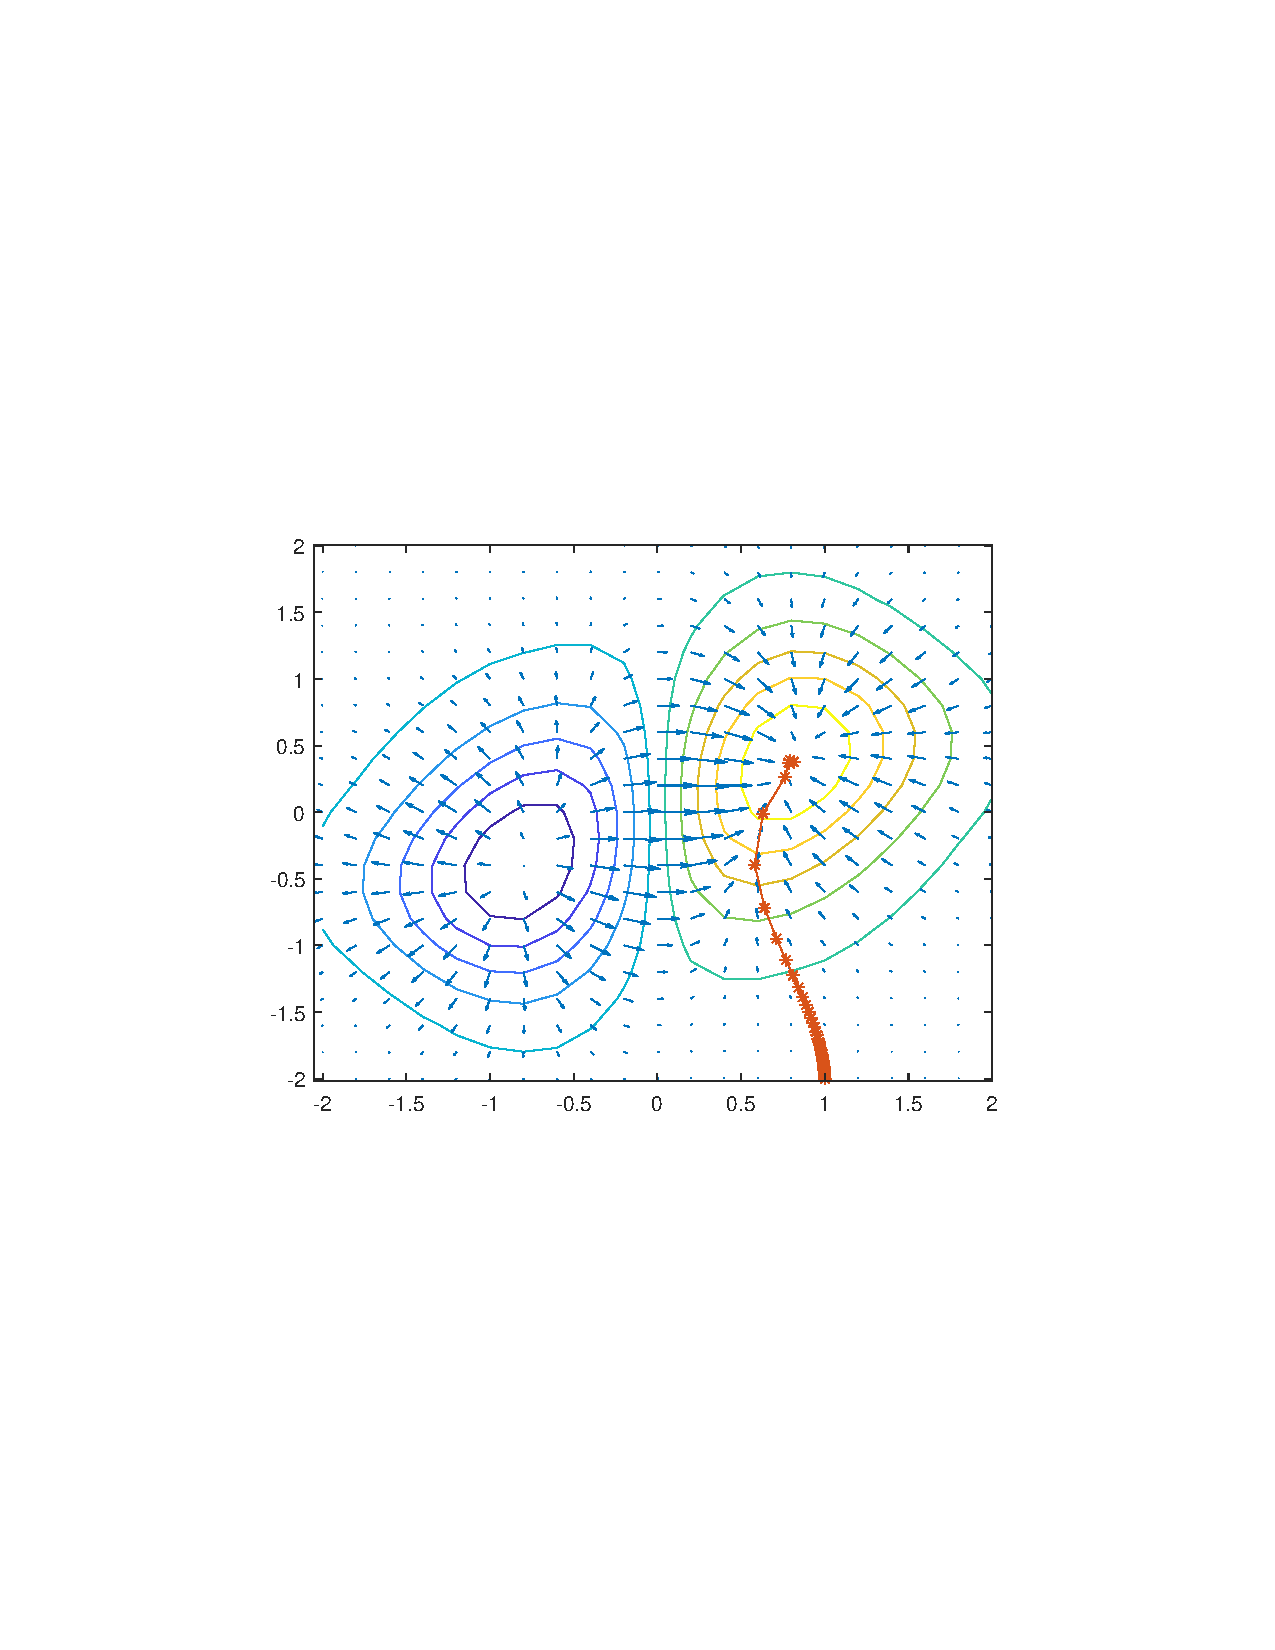
\includegraphics[width=0.49\textwidth, trim = 5cm 9cm 4cm 9cm]{grad_ascent_quiver}}
	{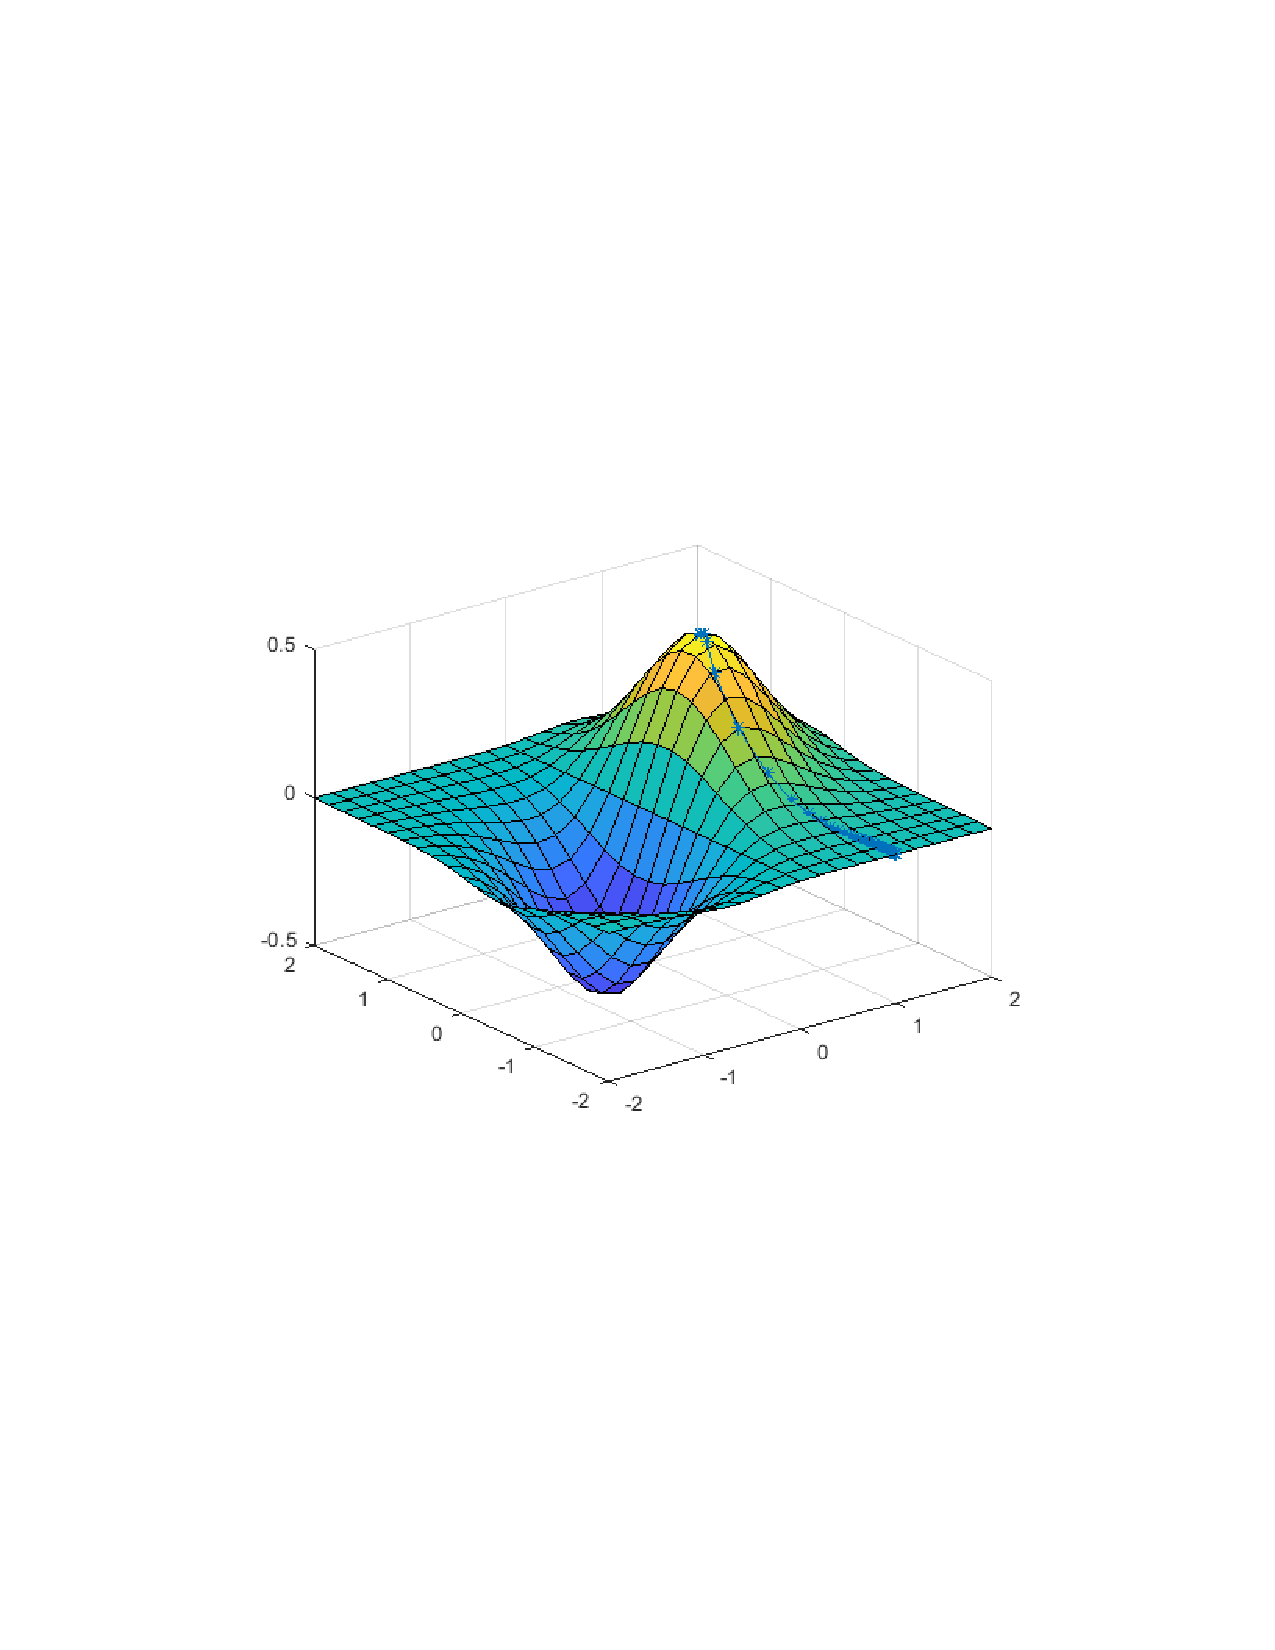
\includegraphics[width=0.49\textwidth, trim = 4cm 9cm 4cm 9cm]{grad_ascent_surf}}
	\caption{Gradient ascent on $f(x_1,x_2) = x_1e^{-x_1^2-x_.^2+\sin(x_1x_2)}$.}
	\label{fig:gradientascent}
\end{figure}
Since the gradient vector field may change from point to point, we can only ``follow" it numerically in finite
steps.  That is, starting from an initial guess $\mathbf{x}_0$,
we generate a sequence of points by the formula
$$
    \mathbf{x}_{n+1} = \mathbf{x}_n + \epsilon \nabla f(\mathbf{x}_n).
$$
The hope then is that
$$
      \mathbf{x}_n  \rightarrow \mathbf{x}^*.
$$
The number $\epsilon$ is often called the ``learning rate". It should not be too small or too large.
 If it is too small the
algorithm will be slow. If it is too large, the steps might skip over a critical point.
There is ongoing research about how to choose it optimally.

Notice the similarities between this method and the Newton's method for nonlinear systems in Lecture~\ref{lec:multnewton}.
In both cases we have a function of a vector and generate a sequence of vectors $\mathbf{x}_0,\mathbf{x}_1,\dots$.

%%%%%%%%%%%%%%%%%%%%%%%%

\subsection*{Exercises}
\begin{list}
  {\arabic{chapter}.\arabic{exercise}}{\usecounter{exercise}}

\item \label{exr:plotquiver}
Find by hand the gradient of the function $f(x_1,x_2) = \sin(x_1) \ e^{-x_1^2 - x_2^2}$. 
   Plot it on the rectangle
  $-3 \le x_1 \le 3$, $-2 \le x_2 \le 2$ using \verb&meshgrid& and \verb&quiver&. 
  On the same figure, add the contour plot of~$f$.


\item  Write a well-commented {\bf script} program that uses the gradient descent method to find a minimum point for the function $f(x_1,x_2) = \sin(x_1) \ e^{-x_1^2 - x_2^2}$, starting from $\mathbf{x}_0 = [-1;-2]$. 
Compare with the plot in exercise \ref{sec:maxmingrad}.\ref{exr:plotquiver} to check that it worked.
(Hint: Review the program \verb*|mymultnewton| in Lecture~\ref{lec:multnewton} for examples of making functions of vectors.)

\end{list}




%%%%%%%%%%%%%%%%%%%%%%%%%%%%%%%%%%%%%%%%%%%%%%%%%%%%%%%%%%%

\chapter{Double Integrals for Rectangles}


%%%%%%%%%%%%%%%%%%%%%%%%%%%%%

\subsection*{The center point method}

Suppose that we need to find the integral of a function,
$f(x,y)$, on a rectangle
$$
    R = \{(x,y): a\le x \le b, c \le y \le d\}.
$$
Calculus tells us to do this by an iterated integral
$$
 I = \iint_R f \, dA = \int_a^b \int_c^d f(x,y) \, dy dx
                   = \int_c^d \int_a^b f(x,y) \, dx dy.
$$
For instance, if $R$ is the rectangle $0 \le x \le 2$, $1 \le y \le 3$, then
\begin{equation*}
\begin{split}
  \iint_R x^2 y \, dA &= \int_0^2 \left(\int_1^3 x^2 y \, dy \right) \, dx \\
           &= \int_0^2  x^2 \left(\left. \frac{y^2}{2} \right|_1^3 \right) \, dx \\
           &= \int_0^2 x^2  \left( \frac{9}{2} - \frac{1}{2} \right) \, dx \\
           &= 4 \int_0^2 x^2 \, dx\\
           &= 4 \cdot \frac{8}{3} = \frac{32}{3} = 10.66... .
\end{split}
\end{equation*}

Calculus also tells us that the integral
is the limit of the  Riemann sums of the function as the size
of the subrectangles goes to zero. This means that the
Riemann sums are approximations of the integral, which is
precisely what we need for numerical methods.

For a rectangle $R$, we begin by subdividing into smaller
subrectangles $\{R_{ij}\}$, in a systematic way. We will divide
$[a,b]$ into $m$ subintervals and $[c,d]$ into $n$ subintervals.
Then $R_{ij}$ will be the ``intersection'' of the $i$-th subinterval
in $[a,b]$ with the $j$-th subinterval of $[c,d]$. In this way
the entire rectangle is subdivided into $mn$ subrectangles, numbered
as in Figure~\ref{rects}.
\begin{figure}
\begin{center}
\setlength{\unitlength}{0.9 mm}
\begin{picture}(83,53)(-3,-3)
	\put(0,0){\line(1,0){80}}
	\put(0,10){\line(1,0){80}}
	\put(0,20){\line(1,0){80}}
	\put(0,30){\line(1,0){80}}
	\put(0,40){\line(1,0){80}}
	\put(0,50){\line(1,0){80}}
	\put(0,0){\line(0,1){50}}
	\put(20,0){\line(0,1){50}}
	\put(40,0){\line(0,1){50}}
	\put(60,0){\line(0,1){50}}
	\put(80,0){\line(0,1){50}}
%
	\put(0,-3){\mbox{$a$}}
	\put(79,-4){\mbox{$b$}}
	\put(-3,0){\mbox{$c$}}
	\put(-3,49){\mbox{$d$}}
%
	\put(5,5){\mbox{$R_{11}$}}
	\put(25,5){\mbox{$R_{21}$}}
	\put(45,5){\mbox{$R_{31}$}}
	\put(65,5){\mbox{$R_{41}$}}
	\put(5,15){\mbox{$R_{12}$}}
	\put(5,25){\mbox{$R_{13}$}}
	\put(5,35){\mbox{$R_{14}$}}
	\put(5,45){\mbox{$R_{15}$}}
	\put(25,15){\mbox{$R_{22}$}}
	\put(25,25){\mbox{$R_{23}$}}
	\put(25,35){\mbox{$R_{24}$}}
	\put(25,45){\mbox{$R_{25}$}}
	\put(45,15){\mbox{$R_{32}$}}
	\put(45,25){\mbox{$R_{33}$}}
	\put(45,35){\mbox{$R_{34}$}}
	\put(45,45){\mbox{$R_{35}$}}
	\put(65,15){\mbox{$R_{42}$}}
	\put(65,25){\mbox{$R_{43}$}}
	\put(65,35){\mbox{$R_{44}$}}
	\put(65,45){\mbox{$R_{45}$}}
\end{picture}
\end{center}
\caption{Subdivision of the rectangle $R = [a,b] \times [c,d]$ into
         subrectangles $R_{ij}$. Note that the arrangement in the $x$-$y$ plane is completely different from the convention in a matrix.}
\label{rects}
\end{figure}

A Riemann sum using this subdivision would have the form 
$$ S =
\sum_{i,j=1,1}^{m,n} f(x^*_{ij}) A_{ij} = \sum_{j=1}^n
\left(\sum_{i=1}^m f(x^*_{ij}) A_{ij}\right)\,, 
$$ where $A_{ij} =
\Delta x_i \Delta y_j$ is the area of $R_{ij}$, and $x^*_{ij}$ is a
point in $R_{ij}$. The theory of integrals tells us that if $f$ is
continuous, then this sum will converge to the same number, no matter
how we choose $x^*_{ij}$. For instance, we could choose $x^*_{ij}$ to
be the point in the lower left corner of $R_{ij}$ and the sum would
still converge as the size of the subrectangles goes to zero. However,
in practice we wish to choose $x^*_{ij}$ in such a way to make $S$ as
accurate as possible even when the subrectangles are not very
small. The obvious choice for the best point in $R_{ij}$ would be the
center point. The center point is most likely of all points to have a
value of $f$ close to the average value of $f$. If we denote the
center points by $c_{ij}$, then the sum becomes
\[ C_{mn} =
\sum_{i,j=1,1}^{m,n} f(c_{ij}) A_{ij}.
\]
Here
\[
 c_{ij} = \left(
\frac{x_{i-1} + x_i}{2}, \frac{y_{i-1} + y_i}{2} \right).
\]
 Note
that if the subdivision is evenly spaced then $\Delta x \equiv
(b-a)/m$ and $\Delta y \equiv (d-c)/n$, and so in that case
\[
 C_{mn}
= \frac{(b-a)(d-c)}{mn} \sum_{i,j=1,1}^{m,n} f(c_{ij}).
\]


%%%%%%%%%%%%%%%%%%

\subsection*{The four corners method}

Another good idea would be to take the value of $f$ not only at one
point, but as the average of the values at several points. An obvious
choice would be to evaluate $f$ at all four corners of each $R_{ij}$
then average those. If we note that the lower left corner is
$(x_i,y_j)$, the upper left is $(x_i,y_{j+1})$,
the lower right is $(x_{i+1},y_i)$ and the upper right is
$(x_{i+1},y_{i+1})$, then the corresponding sum will be
$$
   F_{mn} =   \sum_{i,j=1,1}^{m,n} \frac{1}{4}
            \left( f(x_i,y_j) +
                   f(x_i,y_{j+1}) +
                   f(x_{i+1},y_i) +
                   f(x_{i+1},y_{j+1}) \right)    A_{ij},
$$
which we will call the {\em four-corners} method.
If the subrectangles are evenly spaced, then we can simplify this
expression. Notice that $f(x_i,y_j)$ gets counted multiple
times depending on where $(x_i,y_j)$ is located. For instance
if $(x_i,y_j)$ is in the interior of $R$ then it is the corner
of $4$ subrectangles. Thus the sum becomes
$$
F_{mn} = \frac{A}{4} \left( \sum_{\text{corners}} f(x_i,y_j)
                   + 2 \sum_{\text{edges}} f(x_i,y_j)
                   + 4 \sum_{\text{interior}} f(x_i,y_j)
                         \right),
$$
where $A = \Delta x \, \Delta y$ is the area of the subrectangles.
We can think of this as a weighted average of the values of $f$ at
the grid points $(x_i,y_j)$. The weights used are represented in
the matrix
\begin{equation}\label{dbltrapmatrix}
W = \left( \begin{array}{cccccccc}
           1 & 2 & 2 & 2 & \cdots & 2 & 2 & 1 \\
           2 & 4 & 4 & 4 & \cdots & 4 & 4 & 2 \\
           2 & 4 & 4 & 4 & \cdots & 4 & 4 & 2 \\
        \vdots & \vdots & \vdots & \vdots & \cdots & \vdots & \vdots & \vdots \\
           2 & 4 & 4 & 4 & \cdots & 4 & 4 & 2 \\
           1 & 2 & 2 & 2 & \cdots & 2 & 2 & 1 \\
           \end{array}
    \right).
\end{equation}
We could implement the four-corner method by forming a matrix $(f_{ij})$
of $f$ values at the grid points, then doing entry-wise multiplication
of the matrix with the weight matrix. Then the integral would be
obtained by summing all the entries of the resulting matrix and
multiplying that by $A/4$. The formula would be
$$
     F_{mn} = \frac{(b-a)(d-c)}{4mn} \sum_{i,j = 1,1}^{m+1,n+1}
                       W_{ij} f(x_i,y_j).
$$
Notice that the four-corners method coincides with applying the trapezoid
rule in each direction. Thus it is in fact a {\em double trapezoid}\/ rule.


%%%%%%%%%%%%%%%%%%%%%%%%%%%%

\subsection*{The double Simpson method}

The next improvement one might make would be to take an average of
the center point sum $C_{mn}$ and the four corners sum $F_{mn}$.
However, a more standard way to obtain a more accurate method
is the Simpson double integral. It is obtained by applying Simpson's
rule for single integrals to the iterated double integral.
The resulting method requires that both $m$ and $n$ be even numbers
and the grid be evenly spaced. If this is the case we sum up the
values $f(x_i,y_j)$ with weights represented in the matrix
\begin{equation}\label{dblsimpmatrix}
W = \left( \begin{array}{cccccccc}
           1 & 4 & 2 & 4 & \cdots & 2 & 4 & 1 \\
           4 & 16 & 8 & 16 & \cdots & 8 & 16 & 4 \\
           2 & 8 & 4 & 8 & \cdots & 4 & 8 & 2 \\
           4 & 16 & 8 & 16 & \cdots & 8 & 16 & 4 \\
        \vdots & \vdots & \vdots & \vdots & \cdots & \vdots & \vdots & \vdots \\
           2 & 8 & 4 & 8 & \cdots & 4 & 8 & 2 \\
           4 & 16 & 8 & 16 & \cdots & 8 & 16 & 4 \\
           1 & 4 & 2 & 4 & \cdots & 2 & 4 & 1 \\
           \end{array}
    \right).
\end{equation}
The sum of the weighted values is multiplied by $A/9$ and the formula is
$$
     S_{mn} = \frac{(b-a)(d-c)}{9mn} \sum_{i,j = 1,1}^{m+1,n+1}
                       W_{ij} f(x_i,y_j).
$$


\textsc{Matlab} has a built in command for double integrals on
rectangles: \verb&integral2(f,a,b,c,d)&. Here is an example:
\begin{lstlisting}[frame=none,numbers=left]
f = @(x,y) sin(x.*y)./sqrt(x+y)
I = integral2(f,0.5,1,0.5,2)
\end{lstlisting}
Note that here, as usual, operations are component-wise.

Below is a \textsc{Matlab} function which will produce the
matrix of weights needed for Simpson's rule for double integrals.
It uses the function \verb&mysimpweights& from Lecture~22.


\lstinputlisting{../programs/mydblsimpweights.m}


%%%%%%%%%%%%%%%%


\subsection*{Exercises}
\begin{list}
{\arabic{chapter}.\arabic{exercise}}{\usecounter{exercise}}

\item Download the program \programlink{mylowerleft.m} and test it.
  Find and fix the bug in it.
  Modify it to make a new program \verb&mycenter& that does the center
  point method. Implement the change by changing the ``meshgrid'' to
  put the grid points at the centers of the subrectangles. Look at the
  mesh plot produced to make sure the program is putting the grid
  where you want it. Use both programs to approximate the integral
  $$
  \int_0^2 \int_1^5 \sqrt{xy} \, dy \, dx,
  $$
  using $(m,n) = (10,18)$.  Evaluate this integral exactly (by hand) and compare
  the accuracy of the two programs.

\item Write a well-commented \textsc{Matlab} {\bf function} program
  \verb&mydblsimp& that computes the Simpson's rule approximation. Let
  it call the program \verb&mydblsimpweights& (above) to make the weight
  matrix, $w$ (\ref{dblsimpmatrix}). Check the program on
  the integral in the previous problem using  $(m,n) = (10,18)$ and $(m,n) = (100,100)$.

\item Using \verb&mysimpweights& and \verb&mydblsimpweights& as models
  make well-commented \textsc{Matlab} {\bf function} programs
  \verb&mytrapweights& and \verb&mydbltrapweights& that will produce
  the weights for the trapezoid rule and the weight matrix for the
  four corners (double trapezoid) method (\ref{dbltrapmatrix}). 
  Use it to approximate the integral in the previous problem usings  $(m,n) = (5,6)$ and $(m,n) = (100,100)$.
  Turn in the programs, the weights for a $5\times 6$ grid, and the results of your tests on the integral.

\end{list}

%%%%%%%%%%%%%%%%%%%%%%%%%%%%%%%%%%%%%%%%%%%%%%%%%%%%%%%%%%%%%%%%%

\chapter{Double Integrals for Non-rectangles}


In the previous lecture we considered only integrals over
rectangular regions. In practice, regions of interest are
rarely rectangles and so in this lecture we consider two
strategies for evaluating integrals over other regions.

Calculus tells us that if the region can be described by simple functions,
then we might be able to use iterated integrals. For instance, suppose that
$R$ is the region inside of a circle of radius $2$. Since the boundary of that
circle is given by $x^2 + y^2 = 2^2$,  we could express the
integral of $f(x,y)$ on this region by:
$$
  \int_{-2}^2 \int_{-\sqrt{4-x^2}}^{ \sqrt{4-x^2}} f(x,y) \, dy dx.
$$
Of course this integral may be complicated, even if $f(x,y)$ is simple.
If $f(x,y) = x^2 y^2$, then
\begin{equation*}
\begin{split}
  \int_{-2}^2 \int_{-\sqrt{4-x^2}}^{ \sqrt{4-x^2}} x^2 y^2 \, dy dx 
          &=  \int_{-2}^2 \left. x^2 \frac{y^3}{3} \right|_{-\sqrt{4-x^2}}^{ \sqrt{4-x^2}} \,  dx  \\
          &=  \frac{2}{3} \int_{-2}^2  x^2 (4 - x^2)^\frac{3}{2}  \, dx.     
\end{split}
\end{equation*}
At this point we would need to do a trig substitution to find the value of the integral.

%%%%%%%%%%%%%%%%%%%%%%%%%%%%%

\subsection*{Redefining the function}

One strategy is to redefine the function so that it is zero
outside the region of interest, then integrate over a rectangle
that includes the region.

For example, suppose we need to approximate the value
of
$$
    I = \iint_T \sin^3 (xy) \, dx \, dy
$$
where $T$ is the triangle with corners at $(0,0)$, $(1,0)$ and $(0,2)$.
Then we could let $R$ be the rectangle $[0,1] \times [0,2]$ which
contains the triangle $T$. Notice that the hypotenuse of the triangle
has the equation $2x + y = 2$. Then make $f(x) = \sin^3 (xy)$ if $2x +y \le 2$
and $f(x) = 0$ if $2x+y > 2$.
In \textsc{Matlab} we can make this function with the command
\begin{lstlisting}[frame=none,numbers=left]
f = @(x,y) sin(x.*y).^3.*(2*x + y <= 2)
\end{lstlisting}
In this command \verb&<=& is a {\em logical}\/ command. The term
in parentheses is then a {\em logical statement}\/ and is given the
value 1 if the statement is true and 0 if it is false.
We can then integrate the modified \verb&f& on $[0,1] \times [0,2]$
using the command
\begin{lstlisting}[frame=none,numbers=left]
I = integral2(f,0,1,0,2)
\end{lstlisting}

As another example, suppose we need to integrate the function $f(x,y) = 10+(x-1)(y-2)$
inside the circle of radius 2 centered at $(1,2)$. The equation for
this circle is $(x-1)^2 + (y-2)^2 = 4$. Note that the inside of the
circle is $(x-1)^2 + (y-2)^2 \le 4$ and that the circle is contained
in the rectangle $[-1,3] \times [0,4]$. Thus  we can create
the right function, plot it, and integrate it by
\begin{lstlisting}[frame=none,numbers=left]
f = @(x,y) (10+(x-1).*(y-2)).*((x-1).^2 + (y-2).^2 <= 4)
[X Y] = meshgrid(-4:0.01:4,-3:0.01:5);
Z = f(X,Y);
mesh(X,Y,Z)
I = integral2(f,-1,3,0,4)
\end{lstlisting}

%%%%%%%%%%%%%%%%%%%%%

\subsection*{Integration Based on Triangles}

The second approach to integrating over non-rectangular regions
is based on subdividing the region into triangles. Such a subdivision
is called a {\em triangulation}. On regions
where the boundary consists of line segments, this can be done exactly.
Even on regions where the boundary contains curves, this can be done
approximately. This is a very important idea for several reasons, the
most important of which is that the finite elements method is based on it.
Another reason this is important is that often the values of
$f$ are not given by a formula, but from data.
For example, suppose you are surveying on a construction site
and you want to know how much fill will be needed to bring the
level up to the plan. You would proceed by taking elevations
at numerous points across the site. However, if the site is
irregularly shaped or if there are obstacles on the site, then
you cannot make these measurements on an exact rectangular grid.
In this case, you can use triangles by connecting your points
with triangles. Many software packages will even choose the
triangles for you (\textsc{Matlab} will do it using the command
\verb&delaunay&).

The basic idea of integrals based on triangles is exactly the same
as that for rectangles; the integral is approximated by a sum
where each term is a value times an area
$$
   I \approx \sum_{i=1}^n f(x^*_i) A_i
\,,
$$
where $n$ is the number of triangles, $A_i$ is the area of the triangle
and $x^*$ a point in the triangle. However, rather than considering
the value of $f$ at just one point people often consider an average
of values at several points. The most convenient of these is of course
the corner points. We can represent this sum by
$$
   T_n = \sum_{i=1}^n \bar{f}_i A_i
\,,
$$
where $\bar{f}$ is the average of $f$ at the corners.

If the triangle has vertices $(x_1,y_1)$, $(x_2,y_2)$
and $(x_3,y_3)$,  the formula for area is
\begin{equation}\label{triarea}
A =
\frac{1}{2}\left|
\text{det}\left(
\begin{array}{ccc}
x_1	&x_2	&x_3\\
y_1	&y_2	&y_3\\
1	&1	&1\\
\end{array}
\right)
\right|
% likely wrong, may assume certain differences >0
%A = \frac{1}{2}(x_3 - x_1)(y_2 - y_1) - \frac{1}{2} (y_3 - y_1)(x_2 - x_1)
.
\end{equation}
The function \programlink{mythreecorners.m} below implements this method.
\lstinputlisting{../programs/mythreecorners.m}

Another idea would be to use the center point (centroid) of
each triangle. If the triangle has vertices $(x_1,y_1)$, $(x_2,y_2)$
and $(x_3,y_3)$, then the centroid is given by the simple
formulas
\begin{equation}\label{tricenter}
\bar{x} = \frac{x_1 + x_2 + x_3}{3}
\quad\text{and}\quad
\bar{y} = \frac{y_1 + y_2 + y_3}{3}.
\end{equation}


%%%%%%%%%%%%

\subsection*{Exercises}
\begin{list}
{\arabic{chapter}.\arabic{exercise}}{\usecounter{exercise}}


\item  
   \begin{enumerate}
      \item[a.] Download the program \programlink{mywasher.m}.
      Plot $f(x,y) = \frac{x+y}{x^2+y^2}$ on the region produced  by \programlink{mywasher.m} and 
      use the program \programlink{mythreecorners.m} to calculate the integral of $f$ on the washer.
      Is this accurate? How do you know?
      \item[b.] Download the program \programlink{mywedge.m}.
      Plot $g(x,y) = \sin(x) + \sqrt{y}$ on the region produced  by \programlink{mywedge.m}
      use \programlink{mythreecorners.m} to calculate the integral of $g$ on this wedge.
   \end{enumerate}

\item
  Modify the program \programlink{mythreecorners.m}
  to a new program
\verb&mycenters.m& that does the centerpoint method for triangles. Run
the program on the region produced by \programlink{mywasher.m} with the
function $f(x,y) = \frac{x+y}{x^2+y^2}$ and on the region produced by
\programlink{mywedge.m} with the function $g(x,y) = \sin(x) + \sqrt{y}$.

\end{list}

%
%
%%%%%%%%%%%%%%%%%%%%%%%%%%%%%%%%%%%%%%%%%%%%%%%%%%%%%%%%%%%%%%%%
%
%
%
%\chapter{Gaussian Quadrature*}
%
%
%%%%%%%%%%%%%%%%%%%%%%%%%%%%%%
%
%
%\subsection*{Exercises}
%\begin{list}
%{\arabic{chapter}.\arabic{exercise}}{\usecounter{exercise}}
%
%\item
%
%\vspace*{.2in}
%
%\item
%
%\end{list}
%

%%%%%%%%%%%%%%%%%%%%%%%%%%%%%%%%%%%%%%%%%%%%%%%%%%%%%%

\chapter{Numerical Differentiation}


%%%%%%%%%%%%%%%%%%%%%%%%%%%%%

\subsection*{Approximating derivatives from data}


Suppose that a variable $y$ depends on another variable $x$,
i.e.~$y = f(x)$, but we only know the values of $f$
at a finite set of points, e.g., as data from an experiment
or a simulation:
$$
 (x_1,y_1), (x_2,y_2), \ldots, (x_n,y_n).
$$
Suppose then that we need information about the derivative of $f(x)$.
One obvious idea would be to approximate $f'(x_i)$ by the {\bf Forward
  Difference}
$$
f'(x_i) = y'_i \approx \frac{y_{i+1} - y_i}{x_{i+1}-x_i}.
$$
This formula follows directly from the definition of the derivative in
Calculus.  An alternative would be to use a {\bf Backward Difference}
$$
f'(x_i) \approx \frac{y_i - y_{i-1}}{x_i-x_{i-1}}.
$$

Since the errors for the  forward difference and backward difference tend
to have opposite signs, it would seem likely that averaging the two
methods would give a better result than either alone. If the points are
evenly spaced, i.e.\ $x_{i+1}-x_i = x_i-x_{i-1} = h$, then averaging the
forward and backward differences leads to a symmetric expression called
the {\bf Central Difference}
$$
f'(x_i) = y'_i \approx \frac{y_{i+1} - y_{i-1}}{2h}.
$$
See Figure~\ref{fig:FBCdifferences} for an illustration of these three differences.

\begin{figure}
\centerline{
\includegraphics[width=0.7\textwidth]{differences}}
\caption{The three difference approximations of $y'_i$.}
\label{fig:FBCdifferences}
\end{figure}



%%%%%%%%%%%%%%%%%%%%%%%%%%%%%%


\subsection*{An example}
The following code plots the function $y = \sin(x) + .5\sin(1.5x)$, its derivative, and the central difference approximation to the derivative.

\begin{lstlisting}[frame=none,numbers=left]
x = linspace(0,2*pi,51);
h = x(2)-x(1);
mid = (x(1:end-1)+x(2:end))/2;
y = sin(x) + .5*sin(1.5*x);
dy1 = (y(2:end)-y(1:end-1))/h;
dy2 = cos(x) + .75*cos(1.5*x);
plot(x,y,'k',mid,dy1,'b*',x,dy2,'r')
\end{lstlisting}

%%%%%%%%%%%%%%%%%%%%%%%%%%%%%

\subsection*{Errors of approximation}

We can use Taylor polynomials to derive the accuracy of the forward,
backward, and central difference formulas. For example the usual form
of the Taylor polynomial with remainder (sometimes called Taylor's
Theorem) is
\[ 
f(x+h) = f(x) + h f'(x) + \frac{h^2}{2} f''(c)\,, 
\]
where $c$ is some (unknown) number between $x$ and $x+h$. Letting $x =
x_i$, $x+h = x_{i+1}$ and solving for $f'(x_i)$ leads to
$$ f'(x_i) =
\frac{f(x_{i+1})-f(x_i)}{h} - \frac{h}{2} f''(c).  
$$ 
Notice that the
quotient in this equation is exactly the forward difference formula.
Thus the error of the forward difference is $- (h/2) f''(c)$ which
means it is $O(h)$.  Replacing $h$ in the above calculation by $-h$
gives the error for the backward difference formula; it is also
$O(h)$. For the central difference, the error can be found from the
third degree Taylor polynomials with remainder
\begin{align*}
f(x_{i+1}) &= f(x_i + h)
= f(x_i) + hf'(x_i)+ \frac{h^2}{2} f''(x_i) + \frac{h^3}{3!} f'''(c_1)
\quad\text{and}\\
f(x_{i-1}) &= f(x_i - h)
= f(x_i) - hf'(x_i)+ \frac{h^2}{2} f''(x_i) - \frac{h^3}{3!} f'''(c_2)
\,,
\end{align*}
where $x_i \le c_1 \le x_{i+1}$ and $x_{i-1} \le c_2 \le x_i$.
Subtracting these two equations and solving for $f'(x_i)$ leads to
$$
    f'(x_i) = \frac{f(x_{i+1})-f(x_{i-1})}{2h}
    - \frac{h^2}{3!} \frac{f'''(c_1) + f'''(c_2)}{2}.
$$
This shows that the error for the central difference formula is $O(h^2)$.
Thus, central differences are significantly better and so:
{\bf It is best to use central differences whenever possible.}

There are also central difference formulas for higher order
derivatives. These all have error of order $O(h^2)$:
\begin{align*}
f''(x_i) &=
y''_i \approx \frac{y_{i+1} - 2 y_i + y_{i-1}}{h^2},\\
f'''(x_i) &=
y'''_i \approx \frac{1}{2 h^3} \left[y_{i+2} - 2y_{i+1} + 2y_{i-1} -
y_{i-2} \right] ,\quad\text{and}\\
f^{(4)}(x_i) &= y^{(4)}_i \approx \frac{1}{h^4}
\left[y_{i+2} - 4y_{i+1} + 6y_i - 4y_{i-1} + y_{i-2} \right]
.
\end{align*}

%%%%%%%%%%%%%%%%%%%%%%%%%%%%%

\subsection*{Partial Derivatives}

Suppose $u = u(x,y)$ is a function of two variables that we
only know at grid points $(x_i,y_j)$. We will use the notation
$$
      u_{i,j} = u(x_i,y_j)
$$
frequently throughout the rest of the lectures.
We can suppose that the grid points are evenly spaced, with
an increment of $h$ in the $x$ direction and $k$ in the $y$ direction.
The central difference formulas for the partial derivatives
would be
\begin{align*}
u_x(x_i,y_j) &\approx \frac{1}{2h}
                      \left( u_{i+1,j} - u_{i-1,j} \right)
\quad\text{and}\\
u_y(x_i,y_j) &\approx \frac{1}{2k}
                      \left( u_{i,j+1} - u_{i,j-1} \right).
\end{align*}
The second partial derivatives are
\begin{align*}
u_{xx}(x_i,y_j) &\approx \frac{1}{h^2}
                    \left( u_{i+1,j} -2u_{i,j} + u_{i-1,j} \right)
\quad\text{and}\\
u_{yy}(x_i,y_j) &\approx \frac{1}{k^2}
                    \left( u_{i,j+1} -2u_{i,j} + u_{i,j-1} \right) ,
\end{align*}
and the mixed partial derivative is
$$
    u_{xy}(x_i,y_j) \approx \frac{1}{4hk}
  \left( u_{i+1,j+1} - u_{i+1,j-1} - u_{i-1,j+1} + u_{i-1,j-1} \right) .
$$

{\bf Caution:} Notice that we have indexed $u_{ij}$ so that as a matrix
each row represents the values of $u$ at a certain $x_i$ and each column
contains values at $y_j$. The arrangement in the matrix does not
coincide with the usual orientation of the $xy$-plane.

Let's consider an example. Let the values of $u$ at $(x_i,y_j)$ be
recorded in the matrix
\begin{equation}\label{umatrix}
(u_{ij}) =
 \left( \begin{array}{ccccc}
        5.1 & 6.5 & 7.5 & 8.1 & 8.4 \\
        5.5 & 6.8 & 7.8 & 8.3 & 8.9 \\
        5.5 & 6.9 & 9.0 & 8.4 & 9.1 \\
        5.4 & 9.6 & 9.1 & 8.6 & 9.4
           \end{array} \right)
\end{equation}
Assume the indices begin at 1, $i$ is the index for rows and $j$ the index for columns. Suppose that $h = .5$ and $k = .2$. Then $u_y(x_2,y_4)$ would be
approximated by the central difference
$$
u_y(x_2,y_4) \approx \frac{u_{2,5} - u_{2,3}}{2k}
               \approx \frac{8.9 - 7.8}{2 \cdot 0.2} = 2.75.
$$
The partial derivative $u_{xy}(x_2,y_4)$ is approximated by
$$
u_{xy}(x_2,y_4) \approx \frac{u_{3,5} - u_{3,3} - u_{1,5} + u_{1,3}}{4hk}
               \approx \frac{9.1 - 9.0 - 8.4 + 7.5}{4\cdot .5 \cdot .2}
                 = -2.
$$


%%%%%%%%%%%%%%%%%%%%%%%%%%%%%

\subsection*{Exercises}


\begin{list}
{\arabic{chapter}.\arabic{exercise}}{\usecounter{exercise}}

\item Suppose you are given the data in the following table.\\
\begin{tabular}{c|ccccc}
x & 0 & 5 & 10 & 15 & 20 \\ \hline
y & 0 & 19 & 26 & 29 & 31
\end{tabular}\\
a. Give the forward, backward and central difference approximations of $f'(5)$.\\
b. Give the central difference approximations for $f''(10)$, $f'''(10)$ and
   $f^{(4)}(10)$.
   
\item Suppose the position of a runner was recorded every half second and the results
are given in the following table. Units of distance are meters.\\
\begin{tabular}{c|ccccccccccccc}
t & 0 & .5   & 1.0 & 1.5 & 2.0 & 2.5 & 3.0 & 3.5 & 4.0 & 4.5 & 5.0 & 5.5 & 6.0 \\ \hline
y & 0 & .25 & 1   &   3  & 6    & 10  & 15  & 21  & 27  & 33  &  39  & 45  & 51
 \end{tabular}\\
 Using central differences everywhere possible, and a forward or backward difference where
a central difference is not possible, calculate and plot the velocity and the acceleration of the runner
as a function of time for t=0 to 6. You may do the calculations by hand or by \textsc{Matlab}.  
Turn in your plots and calculations.

\item Suppose values of $u(x,y)$ at points $(x_i,y_j)$ are given in the
matrix (\ref{umatrix}). Suppose that $h = .1$ and $k = .3$.
Approximate the following derivatives by central differences:\\
a. $u_x(x_3,y_4)$\\
b. $u_{xx}(x_2,y_2)$\\
c. $u_{yy}(x_3,y_4)$\\
d. $u_{xy}(x_3,y_3)$


\end{list}




%%%%%%%%%%%%%%%%%%%%%%%%%%%%%%%%%%%%%%%%%%%%%%%%%%%%%%%%%%%%%

\chapter{The Main Sources of Error}

%(not counting bugs)

%%%%%%%%%%%%

\subsection*{Truncation Error}

Truncation error is defined as the error caused directly by an
approximation method. For instance, all numerical integration methods
are approximations and so there is error, even if the calculations are
performed exactly. Numerical differentiation also has a truncation
error, as will the differential equations methods we will study in
Part IV, which are based on numerical differentiation formulas. There
are two ways to minimize truncation error: (1) use a higher order
method, and (2) use a finer grid so that points are closer
together. Unless the grid is very small, truncation errors are usually
much larger than roundoff errors. The obvious tradeoff is that a
smaller grid requires more calculations, which in turn produces more
roundoff errors and requires more running time.

%%%%%%%%%%%%%%%%%%%%%%%%%%

\subsection*{Roundoff Error}

Roundoff error always occurs when a finite number of digits are recorded
after an operation. Fortunately, this error is extremely small. The standard
measure of how small is called {\bf machine epsilon}. It is defined as the
smallest number that can be added to $1$ to produce another number on
the machine, i.e.~if a smaller number is added the result will be rounded
down to $1$. In IEEE standard double precision (used by \textsc{Matlab}
and most serious software), machine epsilon is $2^{-52}$ or about
$2.2 \times 10^{-16}$. A different, but equivalent, way of thinking about
this is that the machine records $52$ floating binary digits or about $15$
floating decimal digits. Thus there are never more than $15$ significant digits
in any calculation. This of course is more than adequate for any application.
However, there are ways in which this very small error
can cause problems.

You can test that machine epsilon is $2^{-52}$:
\begin{lstlisting}[frame=none,numbers=left]
format long
(1 + 2^(-52)) - 1
(1 + 2^(-53)) - 1
\end{lstlisting}
\textsc{Matlab} has a command that produces machine epsilon:
\begin{lstlisting}[frame=none,numbers=left]
eps
\end{lstlisting}
To see an unexpected occurence of round-off try
\begin{lstlisting}[frame=none,numbers=left]
(2^52+1) - 2^52
(2^53+1) - 2^53
\end{lstlisting}
Thus roundoff isn't always small! It is just small compared with the scale of
the numbers you are calculating.
A number of magnitude \(10^p\) will have roundoff of magnitude about \(10^p\cdot 10^{-16}=10^{p-16}\). 

%%%%%%%%%%%%%%%%%%%%%

\subsection*{Loss of Precision (also called Loss of Significance)}

Suppose we had some way
to compute \(\pi\)
that effectively did the calculation
\((e\cdot10^{9}+\pi)-e\cdot10^{9}\). Rounding everything to 16 digits, 
we are computing
\[
(2718281828.459045
+3.141592653589793)
-2718281828.459045\,.
\]
The addition is performed first and the result rounded to 16 digits, giving
\[
 2718281831.600637 %4
-2718281828.459045
\,.
\]
Although roundoff caused some error, it is about a factor of
\(10^{-16}\)
smaller than the numbers shown. In other words, all but perhaps the
last digit shown is correct.
Next the subtraction is performed, giving
\[
 00 00 00 00 03.141592
\,.
\]
The leading zeros are not significant, so we lost 9 significant digits
and have only 7 left.  This type of error, where common leading
significant digits cancel, is loss-of-precision (also called
loss-of-significance) error.
Computers will not display these leading zeros. Instead, the subtraction above yielded  
\[
3.141592025756836
\,.
\]
Although it is displayed with 16 digits, only the first 7 are correct.
%
Usually, if you add two numbers of magnitude \(10^p\) each with roundoff error \(10^{p-16}\), then the result is also of magnitude \(10^p\) and the relative error due to roundoff is \(10^{p-16}/10^p=10^{-16}\).
In this example, cancellation made the result of magnitude \(10^{p-q}\), so the relative error due to roundoff is \(10^{p-16}/10^{p-q}=10^{q-16}\), and so we lost $q=9$ digits of precision.

This type of {\em loss of
  precision}\/ can happen by accident, with catastrophic results, if
you are not careful. For example in $f'(x)\approx (f(x+h)-f(x))/h$ you
will lose precision when $h$ gets too small. Try
\begin{lstlisting}[frame=none,numbers=left]
format long
format compact
f = @(x) x^2
for i = 1:30
   h = 10^(-i)
   df = (f(1+h)-f(1))/h
   relerr = (2-df)/2
end
\end{lstlisting}
At first the relative error decreases since truncation error is reduced. Then
loss of precision takes over and the relative error increases to 1. This happens because when
$f(1)$ and $f(1+h)$ become close, the subtraction ``cancels" digits.


%%%%%%%%%%%%

\subsection*{Bad Conditioning}

We encountered bad conditioning in Part II, when we talked about
solving linear systems.  Bad conditioning means that the problem is
unstable in the sense that small input errors can produce large output
errors. This can be a problem in a couple of ways. First, the
measurements used to get the inputs cannot be completely
accurate. Second, the computations along the way have roundoff
errors. Errors in the computations near the beginning especially can be
magnified by a factor close to the condition number of the matrix.
Thus what was a very small problem with roundoff can become a very big
problem.

It turns out that matrix equations are not the only place where condition
numbers occur. In any problem one can define the condition number
as the maximum ratio of the relative errors in the output versus input, i.e.
$$      \textrm{condition \# of a problem}
          = \max \left( \frac{\text{Relative error of output}}
                             {\text{Relative error of inputs}} \right).
$$
An easy example is solving a simple equation
$$
     f(x) = 0.
$$
Suppose that $f'$ is close to zero at the solution $x^*$. Then a very
small change in $f$ (caused perhaps by an inaccurate measurement of
some of the coefficients in $f$) can cause a large change in $x^*$.
It can be shown that the condition number of this
problem is $1/f'(x^*)$.


\subsection*{Summary}

\begin{table}[hb]
\label{tab:errors}
\begin{tabular}{|c|c|c|}
\hline
\ Error type:  \ & \ Whose fault is it? \ & \ How to mitigate it? \ \\ \hline
\ Truncation \ & \ the method  \  & \ higher-order method or  finer grid \ \\
\ Round-off  \ &  \ the computer  \  & \ usually okay, higher precision arithmetic \ \\ 
\ Loss of Precision \ & \  the programmer \  & \ avoid cancellation of significant digits \  \\
\ Bad Conditioning \ &  \ the problem  \ &  \ check answers, redesign if possible \ \\
\hline
\end{tabular}
\caption{A summary of the main sources of error.}
\end{table}



%%%%%%%%%%%%%%%%
%\subsection*{Build Up}
%
%In addition to these sources of error, there is a another factor
%one must consider that effects the accuracy of calculations: build up.
%Build up can occur when one does multiple calculations
%in the same problem. Each computation may have only a small amount of
%roundoff, truncation or conditioning errors, but adding all the
%small errors up can result in a big error.

%For example, this is one of the trade-offs of using a smaller grid.
%A smaller grid has smaller truncation, but more calculations. At some
%point the advantage is out-weighted by the disadvantage.

%%%%%%%%%%%%

\newpage

\subsection*{Exercises}

\begin{list}
{\arabic{chapter}.\arabic{exercise}}{\usecounter{exercise}}

\item Identify the (main) source of error in each case and propose a
  way to reduce this error if possible.
  \begin{enumerate}
  \item[(a)] If we do $(\sqrt{3})^2$ we should get 3, but if we check
    \begin{lstlisting}[frame=none,numbers=left]
mythree = (sqrt(3))^2
mythree-3
    \end{lstlisting}
    we find the error is 
    \verb&ans = -4.4409e-16&.
  \item[(b)] Since it is a quarter of a circle of radius 2, we should
    have $\int_0^2 \sqrt{4-x^2}dx=\frac{1}{4}\pi2^2=\pi$. We try to
    use \verb&mytrap& from Lecture~\ref{sec:LRTrules} and do
    \begin{lstlisting}[frame=none,numbers=left]
x = 0:.2:2;
y = sqrt(4-x.^2);
mypi = mytrap(x,y)
mypi-pi
    \end{lstlisting}
    and find the error is \verb&ans = -0.0371&.
  \end{enumerate}

\item \footnote{From {\em Numerical Linear Algebra} by L.~Trefethen and D.~Bau, SIAM, 1997.}
%Do the worksheet ``Build-up of Roundoff Errors" from
The function $f(x)=(x-2)^9$ could be evaluated as written, or first
expanded as $f(x)=x^9-18x^8+\cdots$ and then evaluated.
To find the expanded version, type
\begin{lstlisting}[frame=none,numbers=left]
syms x
expand((x-2)^9)
clear
\end{lstlisting}
To evaluate it without expansion, type
\begin{lstlisting}[frame=none,numbers=left]
f1 = @(x) (x-2).^9
x = 1.92:.001:2.08;
y1 = f1(x);
plot(x,y1,'blue')
\end{lstlisting}
To do it with expansion, convert the symbolic expansion above to an anonymous
function \verb&f2& and then type
\begin{lstlisting}[frame=none,numbers=left]
y2 = f2(x);
hold on
plot(x,y2,'red')
\end{lstlisting}
Carefully study the resulting graphs. Should the graphs be the same?
Which is more correct? \textsc{Matlab} does calculations using
approximately 16 decimal places. What is the largest error in the
graph, and how big is it relative to $10^{-16}$? Which source of error
is causing this problem?

\end{list}

%%%%%%%%%%%%%%%%%%%%%%%%%%%%%%%%%%%%%%%%%%%%%%%%%%%

\chapter*{Review of Part III}

\addcontentsline{toc}{chapter}{Review of Part III}
\markboth{REVIEW OF PART III}{}
\subsection*{Methods and Formulas}


\subsubsection*{Polynomial Interpolation:}
An exact fit to the data.\\
For $n$ data points it is a $n-1$ degree polynomial.\\
Only good for very few, accurate data points.\\
The coefficients are found by solving a linear system of equations.

\subsubsection*{Spline Interpolation:}
Fit a simple function between each pair of points.\\
Joining points by line segments is the most simple spline.\\
Cubic is by far the most common and important.\\
Cubic matches derivatives and second derivatives at data points.\\
Simply supported and clamped ends are available.\\
Good for more, but accurate points.\\
The coefficients are found by solving a linear system of equations.

\subsubsection*{Least Squares:}
Makes a ``close fit'' of a simple function to all the data.\\
Minimizes the sum of the squares of the errors.\\
Good for noisy data.\\
The coefficients are found by solving a linear system of equations.


\subsubsection*{Interpolation vs.\ Extrapolation:}
Polynomials, Splines and Least Squares are generally used
for {\em Interpolation}, fitting between the data. {\em Extrapolation},
i.e.\ making fits beyond the data, is much more tricky.
To make predictions beyond the data,
you must have knowledge
of the underlying process, i.e.\ what the function should be.

\subsubsection*{Numerical Integration:}
{\bf Left Endpoint:}
$$
   L_n = \sum_{i=1}^n f(x_{i-1}) \Delta x_i
$$
{\bf Right Endpoint:}
$$
  R_n = \sum_{i=1}^n f(x_i) \Delta x_i .
$$
{\bf Trapezoid Rule:}
$$
T_n = \sum_{i=1}^n \frac{f(x_{i-1}) + f(x_i)}{2} \Delta x_i .
$$
{\bf Midpoint Rule:}
$$
   M_n = \sum_{i=1}^n f(\bar{x}_i) \Delta x_i
\qquad
\textrm{where}
\qquad
        \bar{x}_i = \frac{ x_{i-1} + x_i}{2}.
$$

\subsubsection*{Numerical Integration Rules with Even Spacing:}
For even spacing: $ \Delta x  = \frac{b-a}{n}$
where $n$ is the number of subintervals, then:
$$
   L_n  = \Delta x \sum_{i=0}^{n-1} y_i = \frac{b-a}{n} \sum_{i=0}^{n-1} f(x_i),
$$
$$
   R_n = \Delta x \sum_{i=1}^{n} y_i = \frac{b-a}{n} \sum_{i=1}^n f(x_i),
$$
$$
T_n = \Delta x \bigl( y_0 + 2y_1 + \ldots + 2y_{n-1} + y_n \bigr)
     = \frac{b-a}{2n} \bigl( f(x_0) + 2f(x_1) +
                         \ldots + 2f(x_{n-1}) + f(x_n) \bigr),
$$
$$
   M_n = \Delta x \sum_{i=1}^{n} \bar{y}_i = \frac{b-a}{n} \sum_{i=1}^{n} f(\bar{x}_i),
$$
\subsubsection*{Simpson's rule:}
\begin{align*}
S_n &= \Delta x \bigl( y_0 + 4y_1 + 2y_2 + 4y_3 + \ldots + 2y_{n-2} + 4y_{n-1} + y_n \bigr)\\
    & =  \frac{b-a}{3n} \left( f(x_0) + 4f(x_1) + 2f(x_2) + 4f(x_3) +
            \ldots + 2f(x_{n-2}) + 4f(x_{n-1}) + f(x_n) \right) .
\end{align*}



\subsubsection*{Area of a region:}
\begin{equation*}
   A = - \oint_{C} y \, dx,
\end{equation*}
where $C$ is the counter-clockwise curve around the boundary of the region.
We can represent such a curve, by consecutive points on it, i.e.~
$\bar{x} = (x_0, x_1, x_2, \ldots, x_{n-1}, x_n)$, and
$\bar{y} = (y_0, y_1, y_2, \ldots, y_{n-1}, y_n)$ with $(x_n,y_n) = (x_0,y_0)$.
Applying the trapezoid method to the integral (\ref{areaint}):
$$
    A = - \sum_{i=1}^n \frac{y_{i-1} + y_i}{2} \, (x_i -x_{i-1})
$$

\subsubsection*{Accuracy of integration rules:}
Right and Left endpoint are $O(\Delta x)$\\
Trapezoid and Midpoint are $O(\Delta x^2)$\\
Simpson is $O(\Delta x^4)$


\subsubsection*{Double Integrals on Rectangles:}
{\bf Centerpoint:}
$$
    C_{mn} = \sum_{i,j=1,1}^{m,n} f(c_{ij}) A_{ij}.
$$
where
$$
 c_{ij} = \left( \frac{x_{i-1} + x_i}{2}, \frac{y_{i-1} + y_i}{2} \right).
$$
{\bf Centerpoint -- Evenly spaced:}
$$
    C_{mn} = \Delta x \Delta y \sum_{i,j=1,1}^{m,n} z_{ij} = \frac{(b-a)(d-c)}{mn} \sum_{i,j=1,1}^{m,n} f(c_{ij}).
$$
{\bf Four corners:}
$$
   F_{mn} =   \sum_{i,j=1,1}^{m,n} \frac{1}{4}
            \left( f(x_i,y_j) +
                   f(x_i,y_{j+1}) +
                   f(x_{i+1},y_i) +
                   f(x_{i+1},y_{j+1}) \right)    A_{ij},
$$
{\bf Four Corners -- Evenly spaced:}
\begin{equation*}
\begin{split}
F_{mn} &= \frac{A}{4} \left( \sum_{\text{corners}} f(x_i,y_j)
                   + 2 \sum_{\text{edges}} f(x_i,y_j)
                   + 4 \sum_{\text{interior}} f(x_i,y_j)
                         \right)\\
       &= \frac{(b-a)(d-c)}{4mn} \sum_{i,j = 1,1}^{m,n}
                       W_{ij} f(x_i,y_j).
\end{split}
\end{equation*}
where
$$
W = \left( \begin{array}{cccccccc}
           1 & 2 & 2 & 2 & \cdots & 2 & 2 & 1 \\
           2 & 4 & 4 & 4 & \cdots & 4 & 4 & 2 \\
           2 & 4 & 4 & 4 & \cdots & 4 & 4 & 2 \\
        \vdots & \vdots & \vdots & \vdots & \cdots & \vdots & \vdots & \vdots \\
           2 & 4 & 4 & 4 & \cdots & 4 & 4 & 2 \\
           1 & 2 & 2 & 2 & \cdots & 2 & 2 & 1 \\
           \end{array}
    \right).
$$
{\bf Double Simpson:}
$$
     S_{mn} = \frac{(b-a)(d-c)}{9mn} \sum_{i,j = 1,1}^{m,n}
                       W_{ij} f(x_i,y_j).
$$
where
$$
W = \left( \begin{array}{cccccccc}
           1 & 4 & 2 & 4 & \cdots & 2 & 4 & 1 \\
           4 & 16 & 8 & 16 & \cdots & 8 & 16 & 4 \\
           2 & 8 & 4 & 8 & \cdots & 4 & 8 & 2 \\
           4 & 16 & 8 & 16 & \cdots & 8 & 16 & 4 \\
        \vdots & \vdots & \vdots & \vdots & \cdots & \vdots & \vdots & \vdots \\
           2 & 8 & 4 & 8 & \cdots & 4 & 8 & 2 \\
           4 & 16 & 8 & 16 & \cdots & 8 & 16 & 4 \\
           1 & 4 & 2 & 4 & \cdots & 2 & 4 & 1 \\
           \end{array}
    \right).
$$

\subsubsection*{Integration based on triangles:}
-- Triangulation: Dividing a region up into triangles.\\
-- Triangles are suitable for odd-shaped regions.\\
-- A triangulation is better if the triangles are nearly equilateral.\\
{\bf Three corners:}
$$
   T_n = \sum_{i=1}^n \bar{f}_i A_i
$$
where $\bar{f}$ is the average of $f$ at the corners of the $i$-th triangle.\\
Area of a triangle with corners $(x_1,y_1)$, $(x_2,y_2)$, $(x_3,y_3)$:
\begin{equation*}
A =
\frac{1}{2}\left|
\text{det}\left(
\begin{array}{ccc}
x_1	&x_2	&x_3\\
y_1	&y_2	&y_3\\
1	&1	&1\\
\end{array}
\right)
\right|
.
\end{equation*}
%
{\bf Centerpoint:}
$$
   C = \sum_{i=1}^n f(\bar{x}_i,\bar{y}_i) A_i,
\quad\text{with}
$$
$$
\bar{x} = \frac{x_1 + x_2 + x_3}{3}
\quad\text{and}\quad
 \bar{y} = \frac{y_1 + y_2 + y_3}{3}
\,.
$$

\subsubsection*{Finite Differences}
{\bf Forward Difference}:
$$
f'(x_i) = y'_i \approx \frac{y_{i+1} - y_i}{x_{i+1}-x_i}.
$$
{\bf Backward Difference}:
$$
f'(x_i) \approx \frac{y_i - y_{i-1}}{x_i-x_{i-1}}.
$$
{\bf Central Difference}:
$$
f'(x_i) = y'_i \approx \frac{y_{i+1} - y_{i-1}}{2h}.
$$
{\bf Higher order central differences:}
\begin{align*}
f''(x_i) &= y''_i \approx \frac{y_{i+1} - 2 y_i + y_{i-1}}{h^2},\\
f'''(x_i) &= y'''_i \approx \frac{1}{2 h^3}
		\left[y_{i+2} - 2y_{i+1} + 2y_{i-1} - y_{i-2} \right] ,\\
f^{(4)}(x_i) &= y^{(4)}_i \approx
        \frac{1}{h^4}
    \left[y_{i+2} - 4y_{i+1} + 6y_i - 4y_{i-1} + y_{i-2} \right] .
\end{align*}
%
{\bf Partial Derivatives:}
Denote $ u_{i,j} = u(x_i,y_j)$.
\begin{align*}
u_x(x_i,y_j) &\approx \frac{1}{2h}
                      \left( u_{i+1,j} - u_{i-1,j} \right),\\
u_y(x_i,y_j) &\approx \frac{1}{2k}
                      \left( u_{i,j+1} - u_{i,j-1} \right),\\
u_{xx}(x_i,y_j) &\approx \frac{1}{h^2}
                    \left( u_{i+1,j} -2u_{i,j} + u_{i-1,j} \right) ,\\
u_{yy}(x_i,y_j) &\approx \frac{1}{k^2}
                    \left( u_{i,j+1} -2u_{i,j} + u_{i,j-1} \right) ,\\
u_{xy}(x_i,y_j) &\approx \frac{1}{4hk}
  \left( u_{i+1,j+1} - u_{i+1,j-1} - u_{i-1,j+1} + u_{i-1,j-1} \right) .
\end{align*}


\subsubsection*{Sources of error:}
Truncation -- the method is an approximation.\\
Roundoff -- double precision arithmetic uses $\approx 15$ significant digits.\\
Loss of precision -- an amplification of roundoff error due to cancellations.\\
Bad conditioning -- the problem is sensitive to input errors.\\
Error can build up after multiple calculations.\\

See Table~\ref{tab:errors}.

\subsection*{Matlab}
\subsubsection*{Data Interpolation:}
Use the plot command \verb&plot(x,y,'*')& to plot
the data.\\
Use the Basic Fitting tool to make an interpolation or spline.\\
If you choose an $n-1$ degree polynomial with $n$ data
points the result will be the exact polynomial interpolation.\\
If you select a polynomial degree less than $n-1$, then \textsc{Matlab}
will produce a least squares approximation.

\subsubsection*{Functions of 2 Variables and Meshgrids:}
\verb& f = @(x,y) sin(x.*y)./sqrt(x+y)    &  \dotfill make an anonymous function of $x$ and $y$.\\
\verb& [X Y] = meshgrid(-1:.01:2, 0:.01:3)  & \dotfill make a 2-d grid of points.\\
\verb& Z = f(X,Y) & \dotfill evaluate the function at all points on the grid.\\
\verb& mesh(X,Y,Z) & or \verb& surf(X,Y,Z) &  \dotfill plot the function on the grid.


\subsubsection*{Integration:}
%Numerical integral of $f(x)$ on $[a,b]$:
%\begin{lstlisting}[frame=none,numbers=left]
%integral(f,a,b)
%\end{lstlisting}
%Integral of $f(x,y)$ on $[a,b]\times[c,d]$:
%\begin{lstlisting}[frame=none,numbers=left]
%integral2(f,a,b,c,d)
%\end{lstlisting}
\verb&integral(f,a,b)& \dotfill Numerical integral of $f(x)$ on $[a,b]$.\\
\verb&integral2(f,a,b,c,d)& \dotfill Integral of $f(x,y)$ on $[a,b]\times[c,d]$.\\
Example:
\begin{lstlisting}[frame=none,numbers=left]
f = @(x,y) sin(x.*y)/sqrt(x+y)
I = integral2(f,0,1,0,2)
\end{lstlisting}
\textsc{Matlab} uses an advanced form of Simpson's method.

\subsubsection*{Integration over non-rectangles:}
{\bf Redefine the function} to be zero outside the region. 
For example:
\begin{lstlisting}[frame=none,numbers=left]
f = @(x,y) sin(x.*y).^3.*(2*x + y <= 2)
I = integral2(f,0,1,0,2)
\end{lstlisting}
Integrates $f(x,y) = \sin^3(xy)$ on the triangle with corners $(0,0)$, $(0,2)$, and
$(1,0)$.\\
%


{\bf Triangles:}\\
\textsc{Matlab} stores triangulations as a matrix of vertices
\verb&V& and triangles \verb&T&.
%Produces triangles from vertices:
%\begin{lstlisting}[frame=none,numbers=left]
%T = delaunay(V)  % or delaunay(x,y)
%\end{lstlisting}
%Plots:
%\begin{lstlisting}[frame=none,numbers=left]
%trimesh(T,x,y)
%trimesh(T,x,y,z)
%trisurf(T,x,y)
%trisurf(T,x,y,z)
%\end{lstlisting}
\\
\verb&T = delaunay(V)&  (or \verb& delaunay(x,y)&) \dotfill Produces triangles from vertices.\\
\verb&trimesh(T,x,y) &\\
\verb&trimesh(T,x,y,z) &\\
\verb&trisurf(T,x,y) &\\
\verb&trisurf(T,x,y,z) &


\subsubsection*{Logical expressions}
\verb&(2*x + y <= 2)&, \verb&(x.^2+y.^2<=1)& are examples of logical expressions.\\
If a logical expression is true it is given the value $1$. If false, then it is assigned the value $0$.




%%%%%%%%%%%%%%%%%%%%%%%%%%%%%%%%%%%%%%%%%%%%%%%%%%%%%%%
%%%%%%%%%%%%%%%%%%%%%%%%%%%%%%%%%%%%%%%%%%%%%%%%%%%%%%%
\part{Differential Equations}


%%%%%%%%%%%%%%%%%%%%%%%%%%%%%%%%%%%%%%%%%%%%%%%%%%%%%%%%%
\chapter{Reduction of Higher Order Equations to Systems}


\subsection*{The motion of a pendulum}

Consider the motion of an ideal pendulum that consists of a mass $m$
attached to an arm of length~$\ell$. If we ignore friction,
then Newton's laws of motion tell us
$$
     m \ddot{\theta} = - \frac{mg}{\ell} \sin \theta,
$$
where $\theta$ is the angle of displacement.
\begin{figure}[h]
\begin{center}
\setlength{\unitlength}{0.9 mm}
\begin{picture}(40,40)(0,0)
	\put(0,38){\line(1,0){40}}
	\put(0,38){\line(0,1){2}}
	\put(40,38){\line(0,1){2}}
	\put(20,38){\circle*{2}}
	\put(20,38){\line(1,-2){15}}
	\put(35,8){\circle*{3}}
	\put(20,36){\line(0,-1){2}}
	\put(20,32){\line(0,-1){2}}
	\put(20,28){\line(0,-1){2}}
	\put(20,24){\line(0,-1){2}}
	\put(20,20){\line(0,-1){2}}
	\put(20,16){\line(0,-1){2}}
	\put(20,12){\line(0,-1){2}}
	\put(20,8){\line(0,-1){2}}
	\put(20,4){\line(0,-1){2}}
%
	\put(32,22){\mbox{$\ell$}}
	\put(22,21){\mbox{$\theta$}}
\end{picture}
\end{center}
\caption{A pendulum.}
\end{figure}

If we also incorporate moving friction and sinusoidal forcing
then the equation takes the form
$$
    m \ddot{\theta} + \gamma \dot{\theta} + \frac{mg}{\ell} \sin \theta = A \sin \Omega t.
$$
Here $\gamma$ is the coefficient of friction and $A$ and $\Omega$ are
the amplitude and frequency of the forcing. Usually, this equation
would be rewritten by dividing through by $m$ to produce
\begin{equation}\label{pendulum}
   \ddot{\theta} + c \dot{\theta} + \omega \sin \theta = a \sin \Omega t,
\end{equation}
where $c = \gamma/m$. $\omega = g/\ell$ and $a = A/m$.


This is a second order ODE because the second derivative with respect
to time $t$ is the highest derivative. It is nonlinear because it has
the term $\sin \theta$ and which is a nonlinear function of the
dependent variable $\theta$. A solution of the equation would be a
function $\theta(t)$. To get a specific solution we need side
conditions.  Because it is second order, 2 conditions are needed, and
the usual conditions are initial conditions
\begin{equation}\label{pendulumic}
\theta(0) = \theta_0 \qquad \text{and} \qquad \dot{\theta}(0) = v_0.
\end{equation}

%%%%%%%%%%%%%

\subsection*{Converting a general higher order equation}

All of the standard methods for solving ordinary differential equations
are intended for first order equations. For this reason, it is inconvenient
to solve higher order equations numerically.
However, most higher-order differential equations that
occur in applications can be converted to a {\em system} of
first order equations and that is what is usually done in practice.

Suppose that an $n$-th order equation can be solved for the
$n$-th derivative, i.e. it can be written in the form
\begin{equation*}
x^{(n)} = f\left(t,x,\dot{x},\ddot{x}, \ldots,
                   \frac{d^{n-1}x}{dt^{n-1}}\right).
\end{equation*}
Then it can be converted to a first-order system by this
standard change of variables:
\begin{equation*}
\begin{split}
y_1 &= x\\
y_2 &= \dot{x}\\
   & \vdots \\
y_n & = x^{(n-1)} = \frac{d^{n-1}x}{dt^{n-1}}.
\end{split}
\end{equation*}
The resulting first-order system is
\begin{equation*}
\begin{split}
\dot{y}_1 &= \dot{x} = y_2\\
\dot{y}_2 &= \ddot{x} = y_3\\
   & \vdots \\
\dot{y}_n &= x^{(n)} = f(t,y_1,y_2,\ldots,y_n).
\end{split}
\end{equation*}
In vector form this is simply $\dot{\yb}=\fb(t,\yb)$ with
$f_i(t,\yb)=y_{i+1}$ for $i<n$ and
$f_n(t,\yb)=f(t,y_1,y_2,\ldots,y_n)$.



For the example of the pendulum (\ref{pendulum}) the change of variables
has the form
\begin{equation*}
\begin{split}
y_1 &= \theta\\
y_2 &= \dot{\theta},
\end{split}
\end{equation*}
and the resulting equations are
\begin{equation}\label{pendsys}
\begin{split}
\dot{y}_1 &= y_2\\
\dot{y}_2 &= -c y_2 - \omega \sin(y_1) + a \sin(\Omega t).
\end{split}
\end{equation}
In vector form this is
\[
\dot{\yb}=\left(\begin{array}{c}y_2  \\
		 -c y_2 - \omega \sin(y_1) + a \sin(\Omega t) \end{array} \right).
\]
The initial conditions are converted to
\begin{equation}
\yb(0) = \left(\begin{array}{c} y_1(0) \\ y_2(0) \end{array} \right)
       = \left(\begin{array}{c} \theta_0 \\ v_0 \end{array} \right).
\end{equation}

As stated above, the main reason we wish to change a higher order equation
into a system of equations is that this form is convenient for solving the
equation numerically. Most general software for solving
ODEs (including \textsc{Matlab}) requires that the ODE be input in the form
of a first-order system. In addition, there is a conceptual reason to
make the change. In a system described by a higher order equation, knowing
the position is not enough to know what the system is doing. In the case
of a second order equation, such as the pendulum, one must know both the
angle and the angular velocity to know what the pendulum is really doing.
We call the pair $(\theta, \dot{\theta})$ the
{\em state} of the system. Generally in applications the vector $\yb$ is
the state of the system described by the differential equation.


%%%%%%%%%%%%

\subsection*{Using \textsc{Matlab} to solve a system of ODE's}

In \textsc{Matlab} there are several commands that can be used to
solve an initial value problem for a system of differential equations.
Each of these correspond to different solving methods. The standard
one is \verb&ode45&, which uses the algorithm ``Runge-Kutta 4
5''. We will learn about this algorithm later.

To use \verb&ode45& for a system, we have to input the vector function
$f$ that defines the system, the time span we want to consider and the
initial value of the vector \verb&y&.
%
Suppose we want to solve the pendulum system with \(\omega=a=\Omega=1\)
and $c = .1$ for \(t\in [0,20]\)
with initial condition \((\theta(0),\theta'(0))=(1,-1.5)\).
One way to use \verb&ode45& is to enter
\begin{lstlisting}[frame=none,numbers=left]
dy = @(t,y)[y(2);-.1*y(2)-sin(y(1))+sin(t)]
[T Y] = ode45(dy,[0 20],[1;-1.5]);
\end{lstlisting}
Alternatively, we could create a function program
\begin{lstlisting}
function dy = mypendulum(t,y)
    dy = [y(2);-.1*y(2)-sin(y(1))+sin(t)]
end
\end{lstlisting}
and then enter
\begin{lstlisting}[frame=none,numbers=left]
[T Y] = ode45(@mypendulum,[0 20],[1;-1.5]);
\end{lstlisting}


The output \verb&T& contains times and \verb&Y& contains values of the
vector $\yb$ at those times. Try
\begin{lstlisting}[frame=none,numbers=left]
size(T)
T(1:10)
size(Y)
Y(1:10,:)
\end{lstlisting}
Since the first coordinate of the vector is the position (angle), we
are
mainly interested in its values:
\begin{lstlisting}[frame=none,numbers=left]
theta = Y(:,1)
plot(T,theta)
\end{lstlisting}

In the next two sections we will learn enough about numerical methods
for initial value problems to understand roughly how \textsc{Matlab}
produces this approximate solution.

%%%%%%%%%%%%%%%%%%
\newpage
\subsection*{Exercises}
\begin{list}
{\arabic{chapter}.\arabic{exercise}}{\usecounter{exercise}}

\item Consider the pendulum system  but with no friction or forcing,
i.e. $\gamma = A = 0$. What would equation (\ref{pendsys}) become in this case?
Use the last example to solve the system
with the initial condition $[\theta_0,0]'$ for $\theta_0 = .1\pi$.
Use the plot of the solution to find the frequency of the pendulum
with this initial condition. Do the same for $\theta_0 = .5\pi$ and $.9 \pi$.
How does the frequency depend on the amplitude of a pendulum?



\item Transform the ODE
$$
       \dddot{x} + \ddot{x}^2 - 3\dot{x}^3 + \cos^2{x} = e^{-t} \sin(3t)
$$
 into a first order system.
Suppose the initial conditions for the ODE are
$x(1) = 1$, $\dot{x}(1) = 2$, and $\ddot{x}(1) = 0$.
%What would be the initial condition of the system?
Find a numerical solution of this IVP using \verb&ode45&
and plot the first coordinate ($x$). Try time intervals
%\verb&[1 1.5]&, \verb&[1 1.9]&,
\verb&[1 2]& and \verb&[1 2.1]& and explain
what you observe. 
%(Remember to use entry-wise operations, \verb&.*& and \verb&.^&, in the definition of the vector function.)

\end{list}



%%%%%%%%%%%%%%%%%%%%%%%%%%%%%%%%%%%%%%%%%%%%%%%%%%%%%%%%%%%%%%%%%%%%%%%%%%

\chapter{Euler Methods}

%%%%%%%%%%%%%%%%%%%%%

\subsection*{Numerical Solution of an IVP}

Suppose we wish to numerically solve the initial value problem
\begin{equation}\label{IVP}
\dot{\yb} = \fb(t,\yb), \qquad \yb(a) = \yb_0,
\end{equation}
on an interval of time $[a,b]$.

By a numerical solution, we must mean an approximation of the solution
at a finite number of points, i.e.
$$
(t_0,\yb_0), (t_1,\yb_1), (t_2,\yb_2), \ldots, (t_n,\yb_n),
$$
where $t_0 = a$ and $t_n = b$.
The first of these points is exactly the initial value. If we take
$n$ steps as above, and the steps are evenly spaced, then the time
change in each step is
\begin{equation}\label{hdef}
   h = \frac{b-a}{n},
\end{equation}
and the times $t_i$ are given simply by $t_i = a + ih$.
This leaves the most important part of finding a numerical solution:
determining $\yb_1, \yb_2, \ldots, \yb_n$ in a way that is as consistent
as possible with (\ref{IVP}). To do this, first write the differential
equation in the indexed notation
\begin{equation}\label{DIVP}
    \dot{\yb}_i \approx \fb(t_i,\yb_i),
\end{equation}
and then replace the derivative $\dot{\yb}$ by a
difference. There are many ways we might carry this out and in the
next section we study the simplest.

%%%%%%%%%%%%%%%%%%%%%%%%%%%%%

\subsection*{The Euler Method}

The most straight forward approach is to replace $\dot{\yb}_i$
in (\ref{DIVP}) by its forward difference approximation. This gives
$$
   \frac{\yb_{i+1} - \yb_i}{h} = \fb(t_i,\yb_i).
$$
Rearranging this gives us a way to obtain $\yb_{i+1}$ from $\yb_i$ known
as Euler's method:
\begin{equation}\label{Euler}
\yb_{i+1} = \yb_i + h \fb(t_i,\yb_i).
\end{equation}
With this formula, we can start from $(t_0,\yb_0)$ and compute all the
subsequent approximations $(t_i,\yb_i)$. This is very easy to implement,
as you can see from the following program (which can be downloaded as \programlink{myeuler.m}).
\lstinputlisting{../programs/myeuler.m}

To use this program we need a function, such as the vector function for
the pendulum:
\begin{lstlisting}[frame=none,numbers=left]
dy = @(t,y)[y(2);-.1*y(2)-sin(y(1))+sin(t)]
\end{lstlisting}
Save this  and then type
\begin{lstlisting}[frame=none,numbers=left]
[T Y] = myeuler(dy,[0 20],[1;-1.5],5);
\end{lstlisting}
Here \verb&[0 20]& is the time span you want to consider, \verb&[1;-1.5]& is
the initial value of the vector \verb&y& and \verb&5& is the number of steps.
The output \verb&T& contains times
and \verb&Y& contains values of the vector at the times. Try
\begin{lstlisting}[frame=none,numbers=left]
size(T)
size(Y)
\end{lstlisting}
Since the first coordinate of the vector is the angle, we only plot its values:
\begin{lstlisting}[frame=none,numbers=left]
theta = Y(:,1);
plot(T,theta)
\end{lstlisting}
In this plot it is clear that $n=5$ is not adequate to represent the function.
Type
\begin{lstlisting}[frame=none,numbers=left]
hold on
\end{lstlisting}
then redo the above with 5 replaced by 10. Next try 20, 40, 80, and 200.
As you can see the graph becomes increasingly better as $n$ increases.
We can compare these calculations with \textsc{Matlab}'s built-in function
with the commands
\begin{lstlisting}[frame=none,numbers=left]
[T Y]= ode45(dy,[0 20],[1;-1.5]);
theta = Y(:,1);
plot(T,theta,'r')
\end{lstlisting}

%%%%%%%%%%%%%%%%%%%%%%%%%%

\subsection*{The problem with the Euler method}

You can think of the Euler method as finding a linear approximate
solution to the initial value problem on each time interval.
An obvious shortcoming of the method is that it makes the
approximation based on information at the beginning of the
time interval only. This problem is illustrated well by the
following IVP:
\begin{equation}
   \ddot{x} + x = 0\quad\text{with}\quad 
   x(0)=1\quad\text{and}\quad \dot{x}(0) = 0
\,.
\end{equation}
You can easily check that the exact solution of this IVP is
$$
    x(t) = \cos(t).
$$
If we make the standard change of variables
$$
      y_1 = x \quad\text{and}\quad y_2 = \dot{x},
$$
then we get
$$
       \dot{y}_1 = y_2 \quad\text{and}\quad \dot{y}_2 = - y_1.
$$
Then the solution should be $y_1(t) = \cos(t)$ and $y_2(t) = \sin(t)$.
If we then plot the solution in the $(y_1,y_2)$ plane, we should
get exactly a unit circle. We can solve this IVP with Euler's method:
\begin{lstlisting}[frame=none,numbers=left]
dy = @(t,y)[y(2);-y(1)]
[T Y] = myeuler(dy,[0 4*pi],[1;0],20)
y1 = Y(:,1);
y2 = Y(:,2);
plot(y1,y2)
\end{lstlisting}
As you can see the approximate solution goes far from the true solution.
Even if you increase the number of steps, the Euler solution will
eventually drift outward away from the circle because it does not
take into account the curvature of the solution.

%%%%%%%%%%%%

\subsection*{The Modified Euler Method}

An idea which is similar to the idea behind the trapezoid method
would be to consider $f$ at both the beginning and end of the
time step and take the average of the two. Doing this produces
the Modified (or Improved) Euler method represented by the following
equations:
\begin{equation}
\begin{split}
\mathbf{k}_1 &= h \fb(t_i,\yb_i)\\
\mathbf{k}_2 &= h \fb(t_i+h, \yb_i + \mathbf{k}_1)\\
\yb_{i+1} &= \yb_i +  \frac{1}{2} \left(\mathbf{k}_1 + \mathbf{k}_2 \right)
\,.
\end{split}
\end{equation}
Here $\mathbf{k}_1$ captures the information at the beginning of the
time step (same as Euler), while $\mathbf{k}_2$ is the information at
the end of the time step.

A program that implements the Modified method can be downloaded as
\programlink{mymodeuler.m}.

%\lstinputlisting{../programs/mymodeuler.m}
Test this program on the IVP above:
\begin{lstlisting}[frame=none,numbers=left]
[T Ym] = mymodeuler(dy,[0 4*pi],[1;0],20)
ym1 = Ym(:,1);
ym2 = Ym(:,2);
plot(ym1,ym2)
\end{lstlisting}
You will find that the results are much better than for the plain Euler method.



%%%%%%%%%%%%

\subsection*{Exercises}

\begin{list}
{\arabic{chapter}.\arabic{exercise}}{\usecounter{exercise}}

\item
%Convergence of Euler Methods
Download \programlink{myeuler.m} and  \programlink{mymodeuler.m}.
\begin{enumerate}[(a)]
%\item Create the function:\\ \verb& > dy = @(t,y) sin(t)*cos(y)&\\
\item 
Type the following commands:
\begin{lstlisting}[frame=none,numbers=left]
dy = @(t,y) sin(t)*cos(y);
hold on
[T Y] = myeuler(dy,[0,12],.1,20);
plot(T,Y)
\end{lstlisting}
Position the plot window so that it can always be seen and type
\begin{lstlisting}[frame=none,numbers=left]
[T Y] = myeuler(dy,[0,12],.1,30);
plot(T,Y)
\end{lstlisting}
(You can use the up button to reduce typing.)
Continue to increase the last number in the above until the graph
stops changing (as far as you can see). Record this number and print
the final graph. Type \verb&hold off& and kill the plot window.
\item Follow the same procedure using \programlink{mymodeuler.m} .
\item
Describe what you observed. In particular compare how fast the two
methods converge as $n$ is increased ($h$ is decreased).
\end{enumerate}

\item The equation of motion of a damped, unforced pendulum is
$$   
     \ddot{\theta} + \frac{\gamma}{m} \dot{\theta} + \frac{g}{\ell} \sin \theta = 0.
$$
The total energy of the pendulum is $E = m \ell^2 \dot{\theta}^2/2 + m g \ell (1-\cos(\theta))$.
Suppose a pendulum has $m = 2$, $g = 9.81$, $l = 3$, and coefficient of friction $\gamma = 0.5$, all in SI units.
Write a well-commented {\bf script} program that uses the Modified Euler's method with $h = 0.01$ to simulate the movement of the pendulum from a starting position of
$(\theta(0),\dot{\theta}(0)) = (.9 \pi, 0)$ until the energy falls below 0.01 Joules (use a \verb&while& loop).  
Record the steps in matrices Y and T and plot the motion. Turn in your program and plot.
\end{list}


%%%%%%%%%%%%%%%%%%%%%%%%%%%%%%%%%%%%%%%%%%%%%%%%%%%%%%%%%%%%%%%

\chapter{Higher Order Methods}

%%%%%%%%%%%%%%%%%%%%%

\subsection*{The order of a method}

For numerical solutions of an initial value problem
there are two ways to measure the error. The first
is the error of each step. This is called the Local
Truncation Error or LTE. The other is the total error
for the whole interval $[a,b]$. We call this the
Global Truncation Error or GTE.

For the Euler method the LTE is of order $O(h^2)$, i.e.~the
error is comparable to $h^2$. We can show this directly
using Taylor's Theorem:
$$
    \yb(t+h) = \yb(t) + h \dot{\yb}(t) + \frac{h^2}{2} \ddot{\yb}(c)
$$
for some $c$ between $t$ and $t+h$. In this equation we can replace
$\dot{\yb}(t)$ by $f(t,\yb(t))$, which makes the first two terms
of the right hand side be exactly the Euler method. The error
is then $\frac{h^2}{2} \ddot{\yb}(c)$ or $O(h^2)$.
It would be slightly more difficult to show that the LTE of the
modified Euler method is $O(h^3)$, an improvement of one power of $h$.

We can roughly get the GTE from the LTE by considering the number of steps
times the LTE. For any method, if $[a,b]$ is the interval and $h$ is
the step size, then $n = (b-a)/h$ is the number of steps. Thus for any method,
the GTE is one power lower in $h$ than the LTE. Thus the GTE for Euler
is $O(h)$ and for modified Euler it is $O(h^2)$.

By the {\bf order} of a method, we mean the power of $h$ in the GTE. Thus
the Euler method is a 1st order method and modified Euler is a 2nd order
method.

%%%%%%%%%%%%%%%%%%%%%%%%%%%%%%%%%%%%%%

\subsection*{Fourth Order Runge-Kutta}

The most famous of all IVP methods is the classic Runge-Kutta method
of order 4:
\begin{equation}
\begin{split}
\mathbf{k}_1 &= h \fb(t_i,\yb)\\
\mathbf{k}_2 &= h \fb(t_i+h/2, \yb_i + \mathbf{k}_1/2)\\
\mathbf{k}_3 &= h \fb(t_i+h/2, \yb_i + \mathbf{k}_2/2)\\
\mathbf{k}_4 &= h \fb(t_i+h, \yb_i + \mathbf{k}_3)\\
\yb_{i+1} &= \yb_i + \frac{1}{6} \left(\mathbf{k}_1 + 2 \mathbf{k}_2
                    + 2 \mathbf{k}_3 + \mathbf{k}_4\right).
\end{split}
\end{equation}
Notice that this method uses values of $\fb(t,\yb)$ at $4$ different points.
In general a method needs $n$ values of $\fb$ to achieve order $n$.
The constants used in this method and other methods are obtained
from Taylor's Theorem. They are precisely the values needed to make
all error terms cancel up to $h^{n+1}\fb^{(n+1)}(c)/(n+1)!$.

%%%%%%%%%%%%%%%%%%%%%%%%%%%

\subsection*{Variable Step Size and RK45}

If the order of a method is $n$, then the GTE is
comparable to $h^n$, which means it is approximately $C h^n$,
where $C$ is some constant. However, for different differential
equations, the values of $C$ may be very different. Thus it is
not easy beforehand to tell how small $h$ should be to get
the error within a given tolerence. For instance, if the true
solution oscillates very rapidly, we will obviously need
a smaller step size than for a solution that is nearly constant.

How can a program then choose $h$ small enough to produce
the required accuracy? We also do not wish to make $h$
much smaller than necessary, since that would increase
the number of steps. To accomplish this a program tries
an $h$ and tests to see if that $h$ is small enough.
If not it tries again with a smaller $h$. If it is too
small, it accepts that step, but on the next step it
tries a larger $h$. This process is called {\bf variable step
size}.

Deciding if a single step is accurate enough could be accomplished in
several ways, but the most common are called {\bf embedded methods}.
The Runge-Kutta 45 method, which is used in \verb&ode45&, is an embedded
method. In the RK45, the function
$f$ is evaluated at $5$ different points. These are used to make
a 5th order estimate $\yb_{i+1}$. At the same time, 4 of the 5 values
are used to also get a 4th order estimate. If the 4th order and 5th order
estimates are close, then we can conclude that they are accurate. If
there is a large discrepency, then we can conclude that they are not
accurate and a smaller $h$ should be used.

To see variable step size in action, we will define and solve two different
ODEs and solve them on the same interval.
Create this script and run it:
\begin{lstlisting}
% illustrates variable step size in RK45
dy1 = @(t,y) [-y(2);y(1)];          % create two ODE IVPs
dy2 = @(t,y) [-5*y(2);5*y(1)];
[T1 Y1] = ode45(dy1,[0 20],[1;0]);  % solve with ode45
[T2 Y2] = ode45(dy2,[0 20],[1;0]);
y1 = Y1(:,1);                       % extract position variables
y2 = Y2(:,1);
plot(T1,y1,'bx-')                   % plot both together
hold on
plot(T2,y2,'ro-')
size(T1)                            % print number of steps used
size(T2)
hold off
\end{lstlisting}

%%%%%%%%%%%%%%%%%%%%%%%%%%%%%%%

\subsection*{Why order matters}

Many people would conclude on first encounter that the advantage
of a higher order method would be that you can get a more accurate
answer than for a lower order method. In reality, this is not quite
how things work. In engineering problems, the accuracy needed is
usually a given and it is usually not extremely high.
Thus getting more and more accurate solutions is
not very useful. So where is the advantage? Consider the following example.

Suppose that you need to solve an IVP with an error of less than $10^{-4}$.
If you use the Euler method, which has GTE of order $O(h)$,
then you would need $h \approx 10^{-4}$. So you would need about
$n \approx (b-a) \times 10^4$ steps to find the solution.

Suppose you use the second order, modified Euler method. In that
case the GTE is $O(h^2)$, so you would need to use $h^2 \approx 10^{-4}$, or
$h \approx 10^{-2}$. This would require about $n \approx (b-a) \times 10^2$
steps. That is a hundred times fewer steps than you would need to get
the same accuracy with the Euler method.

If you use the RK4 method, then $h^4$ needs to be approximately $10^{-4}$,
and so $h \approx 10^{-1}$. This means you need only about $n \approx (b-a)\times 10$
steps to solve the problem, i.e. a thousand times fewer steps than for the
Euler method.

Thus the real advantage of higher order methods is that they can run a lot
faster at the same accuracy. This can be especially important in applications
where one is trying to make real-time adjustments based on the calculations.
Such is often the case in robots and other applications with dynamic controls.

%%%%%%%%%%%%%%%%

\subsection*{Exercises}

\begin{list}
{\arabic{chapter}.\arabic{exercise}}{\usecounter{exercise}}


\item There is a Runge-Kutta 2 method, which is also known as the
  midpoint method.  It is summarized by the following equations:
\begin{equation}
\begin{split}
\mathbf{k}_1 &= h \fb(t_i,\yb_i) \\
\mathbf{k}_2 &= h \fb(t_i+h/2, \yb_i + \mathbf{k}_1/2) \\
\yb_{i+1} &= \yb_i + \mathbf{k}_2.
\end{split}
\end{equation}
\begin{enumerate}[(a)]
\item Modify the program \verb&mymodeuler& into a program \verb&myRK2& that
does the RK2 method. 
\item
Test \verb&myRK2& and \verb&mymodeuler& on the
following IVP with time span $[0, 4\pi]$:
$$
     \ddot{x} + x = 0
     \quad\text{with}\quad x(0) = 1\quad\text{and}\quad \dot{x}(0) = 0.
$$
Using \verb&format long&, make a table with \(\yb_{n+1}\) for each of the two programs for
$n = 10$, 100, and 1000. Compute the difference between \(\yb_{n+1}\) and the true solution
$\yb(4\pi)=(1,0)$.
\end{enumerate}
Turn in the modified program and a summary of the results.

\item Consider the initial value problem
\[
  \frac{dy}{dt} = y(t^2-1), \quad y(0)=1.
\]
\begin{enumerate}[(a)]
\item Find the exact solution by hand using Separation of Variables.
\item Solve it by hand using Euler's method  with $h = 0.5$ on the interval $[0,2]$.
\item Solve it using \verb&ode45& on the interval $[0, 2]$.
\item Plot all three solutions on $[0,2]$ in a single plot. Use a continuous curve for the exact solution and symbols at 
the data points for the approximate solutions (e.g.\ '*' for Euler, 'd' for \verb&ode45&).
\item Rank steps (a) - (d) from easiest to hardest.
\end{enumerate}
Turn in your hand work, the plot and your answer to (e). 

\end{list}



%%%%%%%%%%%%%%%%%%%%%%%%%%%%%%%%%%%%%%%%%%%%%%%%%%%%%%%%%%%%%

\chapter{Multi-step Methods*}

%%%%%%%%%%%%%%%%%%%%%

\subsection*{Exercises}
\begin{list}
{\arabic{chapter}.\arabic{exercise}}{\usecounter{exercise}}

\item

\end{list}

%%%%%%%%%%%%%%%%%%%%%%%%%%%%%%%%%%%%%%%%%%%%%%%%%%%%%%%%%%%%%%%%


\chapter{ODE Boundary Value Problems and Finite Differences}

%%%%%%%%%%%%

\subsection*{Steady State Heat and Diffusion}

If we consider the movement of heat in a long thin object (like a metal bar),
it is known that the temperature, $u(x,t)$, at a location $x$
and  time $t$ satisfies the partial differential equation
\begin{equation}\label{heat}
u_t - u_{xx} = g(x,t),
\end{equation}
where $g(x,t)$ is the effect of any external heat source.
The same equation also describes the diffusion of a chemical
in a one-dimensional environment. For example the environment
might be a canal, and then $g(x,t)$ would represent
how a chemical is introduced.

Sometimes we are interested only in the steady
state of the system, supposing $g(x,t) = g(x)$ and $u(x,t) = u(x)$.
In this case
$$
     u_{xx} = -g(x).
$$
This is a linear second-order ordinary differential equation.
We could find its solution exactly if $g(x)$ is not too
complicated. If the environment or object we consider has length
$L$, then typically one would have conditions on each end of
the object, such as $u(0) = 0$, $u(L) = 0$. Thus instead of
an initial value problem, we have a {\bf boundary value problem} or {\bf BVP}.

%%%%%%%%%%%%%%%%

\subsection*{Beam With Tension}

Consider a simply supported beam with modulus of elasticity $E$,
moment of inertia $I$, a uniform load $w$, and
end tension $T$ (see Figure~\ref{fig:beam}). If $y(x)$ denotes
the deflection at each point $x$ in the beam, then $y(x)$
satisfies the differential equation
\begin{equation}\label{beam_non}
\frac{y''}{(1 + (y')^2)^{3/2}} - \frac{T}{EI} y = \frac{wx(L-x)}{2EI},
\end{equation}
with boundary conditions $y(0) = y(L) = 0$.  This equation is
nonlinear and there is no hope to solve it exactly.  If the deflection
is small then $(y')^2$ is negligible compared to 1 and the equation
approximately simplifies to
\begin{equation}\label{beam_lin}
   y'' - \frac{T}{EI} y = \frac{wx(L-x)}{2EI}.
\end{equation}
This is a linear equation and we can find the exact solution.
We can rewrite the equation as
\begin{equation}\label{beam_ab}
 y'' - \alpha y = \beta x(L-x),
\end{equation}
where
\begin{equation}\label{eqn_ab}
\alpha = \frac{T}{EI}  \quad \text{ and } \quad \beta= \frac{w}{2EI},
\end{equation}
and then the exact solution is
\begin{equation}\label{beam_exact}
y(x) = \frac{2\beta}{\alpha^2}
	\frac{e^{\sqrt{\alpha}L}}{e^{\sqrt{\alpha}L}+1} e^{-\sqrt{\alpha}x}
+ \frac{2\beta}{\alpha^2} \frac{1}{e^{\sqrt{\alpha}L}+1} e^{\sqrt{\alpha}x}
          + \frac{\beta}{\alpha} x^2 - \frac{\beta L}{\alpha} x
	+ \frac{2\beta}{\alpha^2}.
\end{equation}
\begin{figure}
\begin{center}
\setlength{\unitlength}{0.9 mm}
\begin{picture}(60,30)(0,0)
	\put(0,5){\line(1,0){10}}
	\put(10,0){\line(0,1){5}}
	\put(50,5){\line(1,0){10}}
	\put(50,0){\line(0,1){5}}
	\put(8,6){\line(1,0){44}}
	\put(8,16){\line(1,0){44}}
	\put(8,6){\line(0,1){10}}
	\put(52,6){\line(0,1){10}}
	\put(8,11){\circle*{2}}
	\put(52,11){\circle*{2}}
	\put(8,11){\vector(-1,0){5}}
	\put(52,11){\vector(1,0){5}}
%
	\put(0,12){\mbox{$T$}}
	\put(57,12){\mbox{$T$}}
%
	\put(10,23){\line(1,0){40}}
	\put(10,23){\vector(0,-1){5}}
	\put(20,23){\vector(0,-1){5}}
	\put(30,23){\vector(0,-1){5}}
	\put(40,23){\vector(0,-1){5}}
	\put(50,23){\vector(0,-1){5}}
	\put(30,25){\mbox{$w$}}
\end{picture}
\end{center}
\caption{A simply supported beam with a uniform load $w$ and
end tension $T$.}
\label{fig:beam}
\end{figure}


%%%%%%%%%%%%%%%%

\subsection*{Finite Difference Method -- Linear ODE}

A finite difference equation is an equation
obtained from a differential equation by replacing
the variables by their discrete versions and
derivatives by difference formulas.

First we will consider equation (\ref{beam_lin}). Suppose that the
beam is a W12x22 structural steel I-beam.  Then $L = 120$ in., $E = 29
\times 10^6 \textrm{lb.}/\textrm{in.}^2$ and $I = 121
\textrm{in.}^4$. Suppose that the beam is carrying a uniform load of $100,000$
lb.\ so that $w = 120,000/120 = 10,000$ and a tension of $T = 10,000$
lb.. We calculate from (\ref{eqn_ab}) $\alpha = 2.850
\times 10^{-6}$ and $\beta = 1.425 \times 10^{-6}$.  Thus we have the
following BVP:
\begin{equation}\label{beam_sim}
  y'' = 2.850 \times 10^{-6} y + 1.425 \times 10^{-6}x(120-x), \qquad y(0) = y(120) = 0.
\end{equation}
First subdivide the interval $[0,120]$ into four equal
subintervals. The nodes of this subdivion
are $x_0 = 0$, $x_1 = 30$, $x_2 = 60$, \ldots, $x_4 = 120$.
We will then let $y_0, y_1, \ldots, y_4$ denote the deflections
at the nodes. From the boundary conditions we have immediately:
$$
   y_0 = y_4 = 0.
$$
To determine the deflections at the interior points we will rely
on the differential equation. Recall the central difference formula
$$
   y''(x_i) \approx \frac{y_{i+1} - 2 y_i + y_{i-1}}{h^2}.
$$
In this case we have $h = (b-a)/n =(120-0)/4= 30$. Replacing all the variables
in the equation (\ref{beam_ab}) by their discrete versions we get
$$
     y_{i+1} - 2 y_i + y_{i-1} = h^2 \alpha y_i + h^2 \beta x_i (L-x_i).
$$
Substituting in for $\alpha$, $\beta$ and $h$ we obtain:
\begin{equation*}
 \begin{split}
     y_{i+1} - 2 y_i + y_{i-1} 
     &= 900 \times 2.850 \times 10^{-6} y_i
     + 900 \times 1.425 \times 10^{-6} x_i(120 - x_i) \\
     &= 2.565 \times 10^{-3} y_i + 1.2825 \times 10^{-3} x_i(120 - x_i).
  \end{split}
\end{equation*}
This equation makes sense for $i = 1,2,3$. At $x_1 = 30$, the equation
becomes:
\begin{equation}
\begin{split}
  y_2 - 2y_1 + y_0
  &= 2.565 \times 10^{-3} y_1+ 1.2825 \times 10^{-3} \times 30(90)\\
  \Leftrightarrow      y_2 -  2.002565 y_1 & = 3.46275.
\end{split}
\end{equation}
Note that this equation is linear in the unknowns $y_1$ and $y_2$.
At $x_2 = 60$ we have:
\begin{equation}
  \begin{split}
    y_3 - 2 y_2 + y_1 
    &= .002565 y_2 + 1.2825 \times 10^{-3} \times 60^2\\
    \Leftrightarrow       y_3 - 2.002565 y_2 + y_1 & = 4.617.
  \end{split}
\end{equation}
At $x_3 = 90$ we have (since $y_4=0$)
\begin{equation}
  \begin{split} % y_4=0
    - 2.002565 y_3 + y_2 &= 3.46275.
  \end{split}
\end{equation}
Thus $(y_1,y_2,y_3)$ is the solution of the linear system:
$$
\left( \begin{array}{ccc|c}
          -2.002565 & 1 & 0 & 3.46275 \\
          1 & -2.002565 & 1 & 4.617 \\
          0 & 1 & -2.002565 & 3.46275
       \end{array}
\right).
$$
We can easily find the solution of this system in \textsc{Matlab}:
\begin{lstlisting}[frame=none,numbers=left]
A = [ -2.002565 1 0 ; 1 -2.002565 1 ; 0 1 -2.002565]
b = [ 3.46275 4.617 3.46275 ]'
y = A\b
\end{lstlisting}
To graph the solution, we need
define the $x$ values and add on the values at the endpoints:
\begin{lstlisting}[frame=none,numbers=left]
x = 0:30:120
y = [0 ; y ; 0]
plot(x,y,'d')
\end{lstlisting}
Adding a spline will result in an excellent graph.

The exact solution of this BVP is given in (\ref{beam_exact}).
That equation, with the parameter values for the W12x22 I-beam
as in the example, is in the program \programlink{myexactbeam.m}.
We can plot the true solution on the same graph:
\begin{lstlisting}[frame=none,numbers=left]
hold on
myexactbeam
\end{lstlisting}
Thus our numerical solution is extremely good considering how
few subintervals we used and how very large the deflection is.

An amusing exercise is to set $T=0$ in the program \programlink{myexactbeam.m};
the program fails because the exact solution is no longer valid. Also
try $T=.1$ for which you will observe loss of precision. On the other hand
the finite difference method still works when we set $T=0$.

%%%%%%%%%%%%%%%%%%
\newpage
\subsection*{Exercises}

\begin{list}
{\arabic{chapter}.\arabic{exercise}}{\usecounter{exercise}}

\item Derive the finite difference equations for the BVP
  (\ref{beam_sim}) on the same domain ($[0,120]$), but with eight
  subintervals and solve (using \textsc{Matlab}) as in the example.
  Plot your result, together on the same plot with the exact solution
  (\ref{beam_exact}) from the program \programlink{myexactbeam.m}.


\item By replacing $y''$ and $y'$ with central differences, derive the
  finite difference equation for the boundary value problem
  $$
  y'' + y' - y = x\quad\text{on $[0,1]$}  \quad\text{with}\quad y(0) = y(1) = 0
  $$
  using 5 subintervals. Solve them and plot the solution using \textsc{Matlab}.
  
  

\end{list}


%%%%%%%%%%%%%%%%%%%%%%%%%%%%%%%%%%%%%%%%%%%%%%%%%%%%%

\chapter{Finite Difference Method -- Nonlinear ODE}

%%%%%%%%%%%%%%%%%%%%%

\subsection*{Heat conduction with radiation}

If we again consider the heat in a metal bar of length $L$, but
this time consider the effect of radiation as well
as conduction, then the steady state equation has the form
\begin{equation}
    u_{xx} - d (u^4 - u_b^4) = - g(x),
\end{equation}
where $u_b$ is the temperature of the background, $d$ incorporates a
coefficient of radiation and $g(x)$ is the heat source.

If we again replace the continuous problem by its discrete approximation
then we get
\begin{equation}\label{condrad}
 \frac{u_{i+1} - 2 u_i + u_{i-1}}{h^2} - d(u_i^4 - u_b^4) = - g_i = -g(x_i).
\end{equation}
This equation is nonlinear in the unknowns, thus we no longer have
a system of linear equations to solve, but a system of nonlinear
equations. One way to solve these equations would be by
the multivariable Newton method in Lecture~\ref{lec:multnewton}. Instead, we introduce another iterative
method.


%%%%%%%%%%%%%%%%%%%%%

\subsection*{Relaxation Method for Nonlinear
                           Finite Differences}

We can rewrite equation (\ref{condrad}) as
$$
u_{i+1} - 2 u_i + u_{i-1} = h^2 d(u_i^4 - u_b^4) - h^2 g_i.
$$
From this we can solve for $u_i$ in terms of the other quantities:
$$
 2 u_i  = u_{i+1} + u_{i-1} - h^2 d(u_i^4 - u_b^4) + h^2 g_i.
$$
Next we add $u_i$ to both sides of the
equation to obtain
$$
 3 u_i  = u_{i+1} + u_i + u_{i-1} - h^2 d(u_i^4 - u_b^4) + h^2 g_i,
$$
and then divide by 3 to get
$$
u_i = \frac{1}{3} \left( u_{i+1} + u_i +  u_{i-1} \right)
     - \frac{h^2}{3} \left( d(u_i^4 - u_b^4) -  g_i \right).
$$

Now for the main idea, we will begin with an initial guess for the
value of $u_i$ for each $i$, which we can represent as a vector
$\ub^0$. Then we will use the above equation to get better
estimates, $\ub^1$, $\ub^2$, \ldots, and hope that they converge
to the correct answer.

If we let
$$
\ub^j = (u_0^j, u_1^j, u_2^j, \ldots, u_{n-1}^j, u_n^j)
$$
denote the $j$th approximation, then we can obtain that $j+1$st estimate
from the formula
$$
 u^{j+1}_i = \frac{1}{3} \left( u^j_{i+1} + u^j_i + u^j_{i-1} \right)
    - \frac{h^2}{3} \left( d((u^j_i)^4 - u_b^4) -  g_i \right).
$$
Notice that $g_i$ and $u_b$ do not change.
In the  resulting equation, we have $u_i$ at each successive step depending
on its previous value and the equation itself.

%%%%%%%%%%%%%%

\subsection*{Implementing the Relaxation Method}

In the following program we solve the finite difference equations
(\ref{condrad}) with the boundary conditions $u(0) = 0$ and $u(L) = 0$.
We let $L = 4$, $n=4$, $d = 1$, and $g(x) = \sin(\pi x/4)$.
Notice that the vector \verb&u& always contains the current estimate of
the values of $\ub$.
\lstinputlisting{../programs/mynonlinheat.m}
If you run this program with the given \verb&n& and \verb&steps& the
result will not seem reasonable.

We can plot the initial guess by adding the command \verb&plot(x,u)&
right before the \verb&for& loop. We can also plot successive
iterations by moving the last \verb&plot(x,u)& before the
\verb&end&. Now we can experiment and see if the iteration is
converging. Try various values of $steps$ and $n$ to produce a good
plot. You will notice that this method converges quite slowly. In
particular, as we increase $n$, we need to increase $steps$ like
$n^2$, i.e.~if $n$ is large then steps needs to be {\em really} large.


\newpage % avoid break in problem

%%%%%%%%%%%%%%

\subsection*{Exercises}
\begin{list}
{\arabic{chapter}.\arabic{exercise}}{\usecounter{exercise}}

\item Modify the script program \verb&mynonlinheat& to plot
    the initial guess and all intermediate approximations. Add
    complete comments to the program.  Print the program
    and a plot using $n = 12$ and \verb&steps& large enough to see
    convergence.
    
\item Modify your improved \verb&mynonlinheat& to
    \verb&mynonlinheattwo& that has the boundary conditions
    $$
    u(0) = 5 \quad\text{and}\quad u(L) = 10.
    $$
    Fix the comments to reflect the new boundary conditions. 
    Print the program and a plot using $n= 50$ and large enough
     \verb&steps& to see convergence.
\end{list}





%%%%%%%%%%%%%%%%%%%%%%%%%%%%%%%%%%%%%%%%%%%%%%%%%%%%%%%%%%%%%

\chapter{Parabolic PDEs - Explicit Method}

%%%%%%%%%%%%%%%%%%%%%

\subsection*{Heat Flow and Diffusion}

In the previous sections we studied PDE that represent {\em steady-state} heat problem.
There was no time variable in the equation. In this section we begin to study how
to solve equations that involve time, i.e.\ we calculate temperature profiles that are
changing.

The conduction of heat and diffusion of a chemical happen to be modeled
by the same differential equation. The reason for this is that
they both involve similar processes. Heat conduction occurs when
hot, fast moving molecules bump into slower molecules and transfer
some of their energy. In a solid this involves moles of molecules
all moving in different, nearly random ways, but the net effect
is that the energy
eventually spreads itself out over a larger region. The diffusion
of a chemical in a gas or liquid simliarly involves large numbers
of molecules moving in different, nearly random ways. These
molecules eventually spread out over a larger region.

In three dimensions, the equation that governs both of these processes
is the heat/diffusion equation
$$
   u_t = c \Delta u
\,,
$$
where $c$ is the coefficient of conduction or diffusion, and $
     \Delta u(x,y,z) = u_{xx} + u_{yy} + u_{zz}$.
The symbol $\Delta$ in this context is called the {\em Laplacian}.
If there is also a heat/chemical source, then it is incorporated
a function $g(x,y,z,t)$ in the equation as
$$
    u_t = c \Delta u + g.
$$

In some problems the $z$ dimension is irrelevant, either because the
object in question is very thin, or $u$ does not change in the $z$
direction. In this case the equation is
$$
   u_t = c \Delta u = c ( u_{xx} + u_{yy}).
$$
Finally, in some cases only the $x$ direction matters. In this case
the equation is just
\begin{equation}\label{1dhd}
    u_t = c u_{xx},
\end{equation}
or
\begin{equation}\label{1dhdn}
    u_t = c u_{xx} + g(x,t).
\end{equation}

In this lecture we will learn a straight-forward technique
for solving (\ref{1dhd}) and (\ref{1dhdn}). It is very
similar to the finite difference method we used for nonlinear
boundary value problems.

It is worth mentioning a related equation
$$
    u_t = c \Delta (u^\gamma)\quad\text{for}\quad\gamma >1
\,,
$$
which is called the porous-media equation.
This equation models diffusion in a solid, but porous, material,
such as sandstone or an earthen structure. We will
not solve this equation numerically, but the methods introduced
here would work. Many equations that involve 1 time derivative
and 2 spatial derivatives are {\bf parabolic} and
the methods introduced here will work for most of
them.

%%%%%%%%%%%%%%

\subsection*{Explicit Method Finite Differences}

The one dimensional heat/diffusion equation $u_t = c u_{xx}$, has two
independent variables, $t$ and $x$, and so we have to discretize both.
Since we are considering $0 \le x \le L$, we subdivide $[0,L]$ into
$m$ equal subintervals, i.e.~let $$ h = L/m $$ and $$ (x_0, x_1, x_2,
\ldots, x_{m-1}, x_m) = (0, h, 2h, \ldots, L-h, L).  $$ Similarly, if
we are interested in solving the equation on an interval of time
$[0,T]$, let $$ k = T/n $$ and $$ (t_0, t_1, t_2, \ldots, t_{n-1},
t_n) = (0, k, 2k, \ldots, T - k, T).  $$ We will then denote the
approximate solution at the grid points by $$ u_{ij} \approx
u(x_i,t_j).  $$

The equation $u_t = c u_{xx}$ can then be replaced by the difference equations
\begin{equation}
\frac{u_{i,j+1} - u_{i,j}}{k} = \frac{c}{h^2} ( u_{i-1,j} - 2 u_{i,j} + u_{i+1,j} ).
\end{equation}
Here we have used the forward difference for $u_t$ and the central
difference for $u_{xx}$.
This equation can be solved for $u_{i,j+1}$ to produce
\begin{equation}\label{expheat}
u_{i,j+1} = r u_{i-1,j} + (1 - 2r) u_{i,j} + r u_{i+1,j}
\end{equation}
for $1 \le i \le m-1$, $0 \le j \le n-1$, where
\begin{equation}
   r = \frac{ck}{h^2}.
\end{equation}
The formula (\ref{expheat}) allows us to calculate all the values
of $u$ at step $j+1$ using the values at step $j$.

Notice that $u_{i,j+1}$ depends on $u_{i,j}$, $u_{i-1,j}$ and
$u_{i+1,j}$. That is $u$ at grid point $i$  depends
on its previous value and the values of its two nearest neighbors
at the previous step (see Figure~\ref{fig:expheat}).

\begin{figure}
\begin{center}
\setlength{\unitlength}{1.5 mm}
\begin{picture}(55,45)(0,0)
	\put(10,10){\circle*{2}}
	\put(20,10){\circle*{2}}
	\put(30,10){\circle*{2}}
	\put(40,10){\circle*{2}}
	\put(50,10){\circle*{2}}
	\put(10,20){\circle*{2}}
	\put(20,20){\circle*{3}}
	\put(30,20){\circle*{3}}
	\put(40,20){\circle*{3}}
	\put(50,20){\circle*{2}}
	\put(10,30){\circle*{2}}
	\put(20,30){\circle*{2}}
%	\put(30,30){\circle{3}}
	\put(27,29){\mbox{$u_{i,j+1}$}}
	\put(40,30){\circle*{2}}
	\put(50,30){\circle*{2}}
	\put(10,40){\circle*{2}}
	\put(20,40){\circle*{2}}
	\put(30,40){\circle*{2}}
	\put(40,40){\circle*{2}}
	\put(50,40){\circle*{2}}
	\put(20,20){\line(1,0){20}}
	\put(30,20){\vector(0,1){7}}
%
	\put(0,18){\mbox{$t_j$}}
	\put(0,28){\mbox{$t_{j+1}$}}
	\put(18,0){\mbox{$x_{i-1}$}}
	\put(28,0){\mbox{$x_i$}}
	\put(38,0){\mbox{$x_{i+1}$}}
\end{picture}
\end{center}
\caption{The value at grid point $(i,j+1)$ depends on its previous value
and the previous values of its nearest neighbors.}
\label{fig:expheat}
\end{figure}

%%%%%%%%%%%%

\subsection*{Initial Condition}

To solve the partial differential equation (\ref{1dhd}) or (\ref{1dhdn})
we need an initial condition. This represents the state of the system when
we begin, i.e. the initial temperature distribution or initial
concentration profile. This is represented by
$$
  u(x,0) = f(x).
$$
To implement this in a program we let
$$
    u_{i,0} = f(x_i).
$$

%%%%%%%%%%%%%%%%%%%%%

\subsection*{Boundary Conditions}

To solve the partial differential equation (\ref{1dhd}) or
(\ref{1dhdn}) we also need boundary conditions. Just as in the
previous section we will have to specify something about the ends of
the domain, i.e. at $x = 0$ and $x = L$. One possibility is fixed
boundary conditions, which we can implement just as we did for the ODE
boundary value problem.

A second possibility is called {\bf variable boundary conditions}.
This is represented by time-dependent functions,
$$
u(0,t) = g_1(t)  \quad\text{and}\quad u(L,t) = g_2(t).
$$
In a heat problem, $g_1$ and $g_2$ would represent heating or cooling
applied to the ends.
These are easily implemented in a program by letting
$u_{0,j} = g_1(t_j)$ and $u_{m,j} = g_2(t_j)$.

%%%%%%%%%%%%

\subsection*{Implementation}

The following program (available to download as \programlink{myheat.m}) implements the
explicit method.  It incorporates variable boundary conditions at both
ends. To run it you must define functions $f$, $g_1$ and $g_2$.
Notice that the main loop has only one line. The values of $u$ are
kept as a matrix. It is often convenient to define a
matrix of the right dimension containing all zeros, and then fill in
the calculated values as the program runs.

Run the following program using $L = 2$, $T=20$, $f(x) = .5 x$, $g_1(t) = 0$,
and $g_2(t) = \cos(t)$. You will find that simply \verb&g1 = @(t) 0& will not
work, because it will only produce a single number $0$. Instead use \verb&g1 = @(t) 0*t&,
which will produce the needed vector of zeros.
\newpage
\lstinputlisting{../programs/myheat.m}

%%%%%%%%%%%%%%%%%%%%%%%%%%%%%%%%%%%%%
\newpage
\subsection*{Exercises}
\begin{list}
{\arabic{chapter}.\arabic{exercise}}{\usecounter{exercise}}


\item Run the program \programlink{myheat.m} with $L = 2\pi$, $T=20$, $c =
  .5$, $g_1(t) = \sin(t)$, $g_2(t) =0$ and $f(x) = -\sin(x/4)$.  Set
  $m=20$ and experiment with $n$. Get a plot when the program is
  stable and one when it isn't. Turn in the plots. Hint: The function $g_2(t)$ will need
  to be input using the formula \verb&g2 = @(t) 0*t&.
  

\item Make a version of the program \programlink{myheat.m} that does not
  input $n$ or $T$ but instead has inputs:
\begin{lstlisting}
%   k -- size of the time steps
%   temp -- keeps stepping in time until the maximum current 
%                 temperature in the bar is less than temp
\end{lstlisting}
For $L = 2\pi$, $c = .01$, $g_1(t) = 0$, $g_2(t) = 10$, $f(x) = 100$
and $m = 10$, set $k$ so that the method will be stable.  Run it with
\verb&temp = 20&.  (Hint: see your Exercise 30.2 as a model.)
{\it When}  does the 
temperature in the bar drop below 20? Turn in your program and the plot.

\end{list}



%%%%%%%%%%%%%%%%%%%%%%%%%%%%%%%%%%%%%%%%%%%%%%%%%%%%%

\chapter{Solution Instability for the Explicit Method}

As we saw in experiments using \programlink{myheat.m}, the solution
can become unbounded unless the time steps are small. In this lecture
we consider why.

%%%%%%%%%%%%%%%%%%%%%

\subsection*{Writing the Difference Equations in Matrix Form}

If we use the boundary conditions $u(0) = u(L) = 0$ then
the explicit method of the previous section has the
form
\begin{equation*}
u_{i,j+1} = r u_{i-1,j} + (1 - 2r) u_{i,j} + r u_{i+1,j}
\quad\text{for}\quad 1 \le i \le m-1\quad\text{and}\quad 0 \le j \le n-1
\,,
\end{equation*}
where $u_{0,j} = 0$ and $u_{m,j} =0$.  This is equivalent to the
matrix equation
\begin{equation}\label{heatev}
     \ub_{j+1} = A \ub_j
\,,
\end{equation}
where $\ub_j$ is the column vector $(u_{1,j}, u_{2,j}, \ldots, u_{m,j})'$
representing the state at the $j$th time step and
$A$ is the matrix
\begin{equation}\label{heatmat}
A = \left( \begin{array}{ccccc}
          1-2r & r      &   0     & \cdots   &  0 \\
            r  & 1-2r   & r      &  \ddots   &  \vdots \\
            0   & \ddots & \ddots & \ddots & 0  \\
            \vdots   &  \ddots &   r    & 1-2r   & r \\
            0   & \cdots       &  0      &   r    & 1-2r
            \end{array}
     \right).
\end{equation}
Unfortunately, this matrix can have a property which is very bad in
this context. Namely, it can cause exponential growth of error
unless $r$ is small. To see how this happens, suppose that
$\Ub_j$ is the vector of correct values of $u$ at
time step $t_j$ and $\Eb_j$ is the error of the approximation
$\ub_j$, then
$$
      \ub_j = \Ub_j + \Eb_j.
$$
From (\ref{heatev}), the approximation at the next time step will be
$$
    \ub_{j+1} = A \Ub_j + A \Eb_j,
$$
and if we continue for $k$ steps,
$$
    \ub_{j+k} = A^k \Ub_j + A^k \Eb_j.
$$
The problem with this is the term $A^k \Eb_j$. This term
is exactly what we would do in the power method for finding
the eigenvalue of $A$ with the largest absolute value. If the
matrix $A$ has eigenvalues with absolute value greater than $1$,
then this term will grow exponentially. Figure~\ref{heatspec}
shows the largest absolute value of an eigenvalue of $A$ as a function
of the parameter $r$ for various sizes of the matrix $A$.
As you can see, for $r> 1/2$ the largest absolute eigenvalue grows rapidly
for any $m$ and quickly becomes greater than $1$.


\begin{figure}
\centerline{

\includegraphics[width=0.6\textwidth]{heatspec}}
\caption{Maximum absolute eigenvalue as a function of $r$ for the
matrix $A$ from the explicit method for the heat equation
calculated for matrices $A$ of sizes $m = 2 \ldots 10$.
Whenever the maximum absolute eigenvalue is greater than 1 the method is unstable, i.e.\ errors grow exponentially with
each step. When using the explicit method $r < 1/2$ is a safe choice.}
\label{heatspec}
\end{figure}

%%%%%%%%%%%

\subsection*{Consequences}

Recall that $r = ck/h^2$. Since this must be less than 1/2, we have
$$
        k < \frac{h^2}{2c}.
$$
The first consequence is obvious: $k$ must be relatively small.
%
The second is that $h$ cannot be too small. Since $h^2$ appears
in the formula, making $h$ small would force $k$ to be extremely
small!
%
A third consequence is that we have a converse of this
analysis. Suppose $r < .5$.
Then all the eigenvalues will be less than one. Recall that
the error terms satisfy
$$
    \ub_{j+k} = A^k \Ub_j + A^k \Eb_j.
$$
If all the eigenvalues of $A$ are less than $1$ in absolute value then
$A^k \Eb_j$ grows smaller and smaller as $k$ increases. This
is really good. Rather than building up, the effect of any
error diminishes as time passes! From this we arrive at the following
principle: {\bf If the explicit numerical solution for a parabolic
equation does not blow up, then errors from previous steps fade away!}

Finally, we note that if we have non-zero boundary conditions
then instead of equation (\ref{heatev}) we have
\begin{equation}\label{heatev2}
     \ub_{j+1} = A \ub_j + r \bb_j,
\end{equation}
where the first and last entries of $\bb_j$ contain the boundary
conditions and all the other entries are zero. In this case the
errors behave just as before, if
$r> 1/2$ then the errors grow and if $r<1/2$ the errors
fade away.


We can write a function program \programlink{myexpmatrix.m} that produces the matrix
$A$ in (\ref{heatmat}), for given inputs $m$ and $r$.  Without using loops
we can use the \verb&diag& command to
set up the matrix:
\lstinputlisting{../programs/myexpmatrix.m}
Test this using $m=6$ and $r=.4, .6$. Check the eigenvalues and
eigenvectors of the resulting matirices:
\begin{lstlisting}[frame=none,numbers=left]
A = myexpmatrix(6,.6)
[v e] = eig(A)
\end{lstlisting}
What is the ``mode'' represented by the eigenvector with the largest absolute
eigenvalue? How is that reflected in the unstable solutions?

%%%%%%%%%%%

\subsection*{Exercises}

\begin{list}
{\arabic{chapter}.\arabic{exercise}}{\usecounter{exercise}}

\item Let $L=\pi$, $T = 20$, $f(x) = .1\sin(x)$, $g_1(t) = 0$, $g_2(t)
  = 0$, $c = .5$, and $m = 20$, as used in the program
  \programlink{myheat.m}.  What value of $n$ corresponds to $r =
  1/2$?  Try different $n$ in \programlink{myheat.m} to find precisely when
  the method works and when it fails. Is $r = 1/2$ the boundary
  between failure and success?  Hand in a plot of the last success and
  the first failure. Include the values of $n$ and $r$ in each.

\item Write a well-commented \textsc{Matlab} {\bf script}
  program that produces the graph in
  Figure~\ref{heatspec} for $m = 4$. Your program should: 
  \begin{itemize}
  \item define $r$ values from $0$ to $1$,
  \item for each $r$ 
    \begin{itemize}
    \item create the matrix $A$ by calling \verb&myexpmatrix&,
    \item calculate the eigenvalues of $A$,
    \item find the max of the absolute values, and
    \end{itemize}
  \item plot these numbers versus $r$.
  \end{itemize}

\end{list}


%%%%%%%%%%%%%%%%%%%%%%%%%%%%%%%%%%%%%%%%%%%%%%%%%%%%%%%%%%%%%%%

\chapter{Implicit Methods}

%%%%%%%%%%%%%%%%%%%%%

\subsection*{The Implicit Difference Equations}

By approximating $u_{xx}$ and $u_t$ at $t_{j+1}$ rather than $t_j$,
and using a backwards difference for $u_t$, the equation $u_t = c
u_{xx}$ is approximated by
\begin{equation*}
\frac{u_{i,j+1} - u_{i,j}}{k} 
= \frac{c}{h^2} ( u_{i-1,j+1} - 2 u_{i,j+1} + u_{i+1,j+1} ).
\end{equation*}
Note that all the terms have index $j+1$ except one and isolating this term
leads to
\begin{equation}
\label{eqn:impheatstencil}
u_{i,j} = -r u_{i-1,j+1} + (1+2r) u_{i,j+1} - r u_{i+1,j+1}
\quad\text{for}\quad 1 \le i \le m-1,
\end{equation}
where $r = ck/h^2$ as before.
The entries involved in (\ref{eqn:impheatstencil}) are illustrated in Figure~\ref{fig:impheat}.
\begin{figure}
\begin{center}
\setlength{\unitlength}{1.5 mm}
\begin{picture}(55,45)(0,0)
	\put(10,10){\circle*{2}}
	\put(20,10){\circle*{2}}
	\put(30,10){\circle*{2}}
	\put(40,10){\circle*{2}}
	\put(50,10){\circle*{2}}
	\put(10,20){\circle*{2}}
	\put(20,20){\circle*{2}}
	%\put(30,20){\circle*{2}}
	\put(27,19){\mbox{$u_{i,j}$}}
	\put(40,20){\circle*{2}}
	\put(50,20){\circle*{2}}
	\put(10,30){\circle*{2}}
	\put(20,30){\circle*{3}}
	\put(30,30){\circle*{3}}
	\put(40,30){\circle*{3}}
	\put(50,30){\circle*{2}}
	\put(10,40){\circle*{2}}
	\put(20,40){\circle*{2}}
	\put(30,40){\circle*{2}}
	\put(40,40){\circle*{2}}
	\put(50,40){\circle*{2}}
	\put(20,30){\line(1,0){20}}
	\put(30,30){\vector(0,-1){7}}
%
	\put(0,18){\mbox{$t_j$}}
	\put(0,28){\mbox{$t_{j+1}$}}
	\put(18,0){\mbox{$x_{i-1}$}}
	\put(28,0){\mbox{$x_i$}}
	\put(38,0){\mbox{$x_{i+1}$}}
\end{picture}
\end{center}
\caption{The value at grid point $(i,j)$ depends on its future value
and the future values of its nearest neighbors.}
\label{fig:impheat}
\end{figure}




Now we have $\ub_j$ given in terms of $\ub_{j+1}$.  This seems like a
problem, since $\ub_{j+1}$ is the solution at a later time than
$\ub_j$, so we could never know $\ub_{j+1}$ before we knew $\ub_j$.
However, the relationship between $\ub_{j+1}$ and $\ub_j$
is linear.
Using matrix notation, we have
$$
     \ub_j = B \ub_{j+1} - r \bb_{j+1},
$$
where $\bb_{j+1}$ represents the boundary conditions. Thus to
find $\ub_{j+1}$ from $\ub_j$, we need only solve the linear system
\begin{equation}\label{impheatev}
      B \ub_{j+1} = \ub_j + r \bb_{j+1}
\,,
\end{equation}
where $\ub_j$ and $\bb_{j+1}$ are given and
\begin{equation}\label{impheatmat}
B = \left( \begin{array}{ccccc}
          1+2r &  -r    &        &        &   \\
           -r  &  1+2r  &  -r    &        &   \\
               & \ddots & \ddots & \ddots &   \\
               &        &  -r    & 1+2r   & -r\\
               &        &        &   -r   & 1+2r
            \end{array}
     \right).
\end{equation}
 (This is an example of
how a sparse matrix occurs in applications.)
Using this scheme is called the {\bf implicit method} since
$\ub_{j+1}$ is defined implicitly. 
Since we have to solve a linear
system at each step, the implicit method requires more work per step than the explicit method. 

Since we are solving (\ref{impheatspec}), the most important
quantity is the maximum absolute eigenvalue of $B^{-1}$, which
is 1 divided by the smallest eigenvalue of $B$.
Figure~\ref{impheatspec} shows the maximum absolute eigenvalues of
$B^{-1}$ as a function of $r$ for various size matrices.
\begin{figure}
%\centerline{\hbox{
\psfig{figure=impheatspec.eps,height=3in,width=3.2in}}}
\centerline{
\includegraphics[width=0.65\textwidth]{impheatspec}}
\caption{Maximum absolute eigenvalue as a function of $r$ for the
matrix $B^{-1}$ from the implicit method for the heat equation
calculated for matrices $B$ of sizes $m = 2 \ldots 10$.
Whenever the maximum absolute eigenvalue is less than 1 the method is stable, i.e. it is always stable.}
\label{impheatspec}
\end{figure}
Notice that this absolute maximum is always less than $1$.
Thus errors are always diminished over time and so this
method is always stable. For the same reason it is also
always as accurate as the individual steps.

Both this implicit method and the explicit method in the previous
lecture make $O(h^2)$ error in approximating $u_{xx}$ and $O(k)$ error
in approximating $u_t$, so they have total error $O(h^2+k)$. Thus
although the stability condition allows the implicit method to use
arbitrarily large $k$, to maintain accuracy we still need $k\sim h^2$.

%%%%%%%%%%%%%

\subsection*{Crank-Nicholson Method}

Now that we have two different methods for solving parabolic
equation, it is natural to ask, ``can we improve by taking
an average of the two methods?'' The answer is yes.

We implement a weighted average of the two methods by considering
an average of the approximations of $u_{xx}$ at $j$ and $j+1$.
This leads to the equations
\begin{equation}
\frac{u_{i,j+1} - u_{i,j}}{k}
= \frac{\lambda c}{h^2} ( u_{i-1,j+1} - 2 u_{i,j+1} + u_{i+1,j+1} )
+  \frac{(1-\lambda) c}{h^2} ( u_{i-1,j} - 2 u_{i,j} + u_{i+1,j} ).
\end{equation}
The implicit method contained in these equations is called the
{\bf Crank-Nicholson method}.
Gathering terms yields the equations
$$
  -r \la u_{i-1,j+1} + (1+2r\la) u_{i,j+1} - r\la u_{i+1,j+1}
       = r(1-\la) u_{i-1,j} + (1 - 2r(1-\la)) u_{i,j} + r(1-\la) u_{i+1,j}.
$$
In matrix notation this is
$$
   B_\la \ub_{j+1} = A_\la \ub_j + r\bb_{j+1},
$$
where
\begin{equation*}
A_\la = \left( \begin{array}{ccccc}
          1-2(1-\la)r & (1-\la)r &        &        &   \\
            (1-\la)r  & 1-2(1-\la)r & (1-\la)r &        &   \\
                      & \ddots      & \ddots & \ddots &   \\
                      &             & (1-\la)r & 1-2(1-\la)r   & (1-\la)r \\
                      &             &          &   (1-\la)r    & 1-2(1-\la)r
            \end{array}
     \right)
\end{equation*}
and
\begin{equation*}
B_\la = \left( \begin{array}{ccccc}
          1+2r\la &  -r\la    &        &        &   \\
           -r\la  &  1+2r\la  &  -r\la    &        &   \\
               & \ddots & \ddots & \ddots &   \\
               &        &  -r\la    & 1+2r\la   & -r\la\\
               &        &        &   -r\la   & 1+2r\la
            \end{array}
     \right).
\end{equation*}
In this equation $\ub_j$ and $\bb_{j+1}$ are known, $A \ub_j$ can be
calculated directly, and then the equation is solved for $\ub_{j+1}$.

If we choose $\lambda=1/2$, then we are in effect doing a central
difference for $u_t$, which has error $O(k^2)$. Our total error is
then $O(h^2+k^2)$.  With a bit of work, we can show that the method is
always stable, and so we can use $k\sim h$ without a problem.

To get optimal accuracy with a weighted average, it is always
necessary to use the right weights. For the Crank-Nicholson
method with a given $r$, we need to choose
$$
    \lambda = \frac{r - 1/6}{2r}.
$$
This choice will make the method have truncation error of order
$O(h^4 + k^2)$, which is really good considering that the implicit and
explicit methods each have truncation errors of order $O(h^2 + k)$.
Surprisingly, we can do even better if we also require
$$
    r = \frac{\sqrt{5}}{10} \approx 0.22361,
$$
and, consequently,
$$
    \la = \frac{3 - \sqrt{5}}{6} \approx  0.12732.
$$
With these choices, the method has truncation error of order $O(h^6)$,
which is absolutely amazing.

To appreciate the implications, suppose that we need to solve
a problem with 4 significant digits. If we use the explicit or
implicit method alone then we will need $h^2 \approx k \approx 10^{-4}$.
If $L=1$ and $T\approx 1$, then we need
$m \approx 100$ and $n \approx 10,000$. Thus we would have a total
of $1,000,000$ grid points, almost all in the interior. This is a lot.

Next suppose we solve the same problem using the optimal
Crank-Nicholson method. We would need $h^6 \approx 10^{-4}$ which
would require us to take $m \approx 4.64$, so we would take $m = 5$
and have $h=1/5$. For $k$ we need $k = (\sqrt{5}/10) h^2/c$. If $c=1$,
this gives $k = \sqrt{5}/250\approx 0.0089442$ so we would need
$n\approx 112$ to get $T\approx 1$. This gives us a total of $560$
interior grid points, or, a factor of $1785$ fewer than the explicit or
implicit method alone.


%%%%%%%%%%%%%

\subsection*{Exercises}

\begin{list}
{\arabic{chapter}.\arabic{exercise}}{\usecounter{exercise}}

\item
Modify the program \programlink{myexpmatrix.m} from exercise 36.2 into a
function program \verb&myimpmatrix.m& that produces the matrix $B$ 
in (\ref{impheatmat})
for given inputs $m$ and $r$. Modify your script from exercise
36.2 to use $B^{-1}$ and to plot for \(r\in[0,2]\); keep $m = 4$. It should produce a
graph similar to that in Figure~\ref{impheatspec} for $m = 4$. Turn in the
programs and the plot.

\item
Modify the program \verb&myheat& into a new program \verb&myimplicitheat&
that uses the implicit method to solve the boundary value problem
$$
    u_t = c u_{xx}, \quad u(t,0) = u(t,L) = 0, \quad u(0,x) = f(x)
$$
by repeatedly solving the system $B \ub_{j+1} = \ub_j$ for each time step.

(Hints: Delete \verb&g1& and \verb&g2& from the program
since they are always zero. Call $B$ using \verb&myimpmatrix& before the
loop and solve $B \ub_{j+1} = \ub_j$ inside the loop.)
%Once the program is working, change  it to calculate the LU decomposition of $B$ before the loop and use the LU to solve $B \ub_{j+1} = \ub_j$ inside the loop. 

Run the program with $L=5$, $T=50$, $c=.1$ and $f(x) = \sin( \pi x/5)$ and at least 10 pairs
of values of $m$ and $n$. Turn in the program and a list of the $m,n$ you tried
and whether the simulation was stable or unstable. Are you convinced that it is 
always stable?


    


\end{list}



%%%%%%%%%%%%%%%%%%%%%%%%%%%%%%%%%%%%%%%%%%%%%%%%%%%%%%%

\chapter{Insulated Boundary Conditions}

%%%%%%%%%%%%%%%%%%%%%%%%%%%%%

\subsection*{Insulation}

In many of the previous sections we have considered fixed boundary
conditions, i.e.~$u(0) = a$, $u(L) = b$.  We implemented these simply
by assigning $u_0^j =a$ and $u_n^j = b$ for all $j$.

We also considered variable boundary conditions, such as $u(0,t) =
g_1( t)$.  For example, we might have $u(0,t) = \sin( t)$ which could
represent periodic heating and cooling of the end at $x=0$.

A third important type of boundary condition is called the {\em
  insulated} boundary condition. It is so named because it mimics an
insulator at the boundary.  Physically, the effect of insulation is
that no heat flows across the boundary.  This means that the
temperature gradient is zero, which implies that we should require the
mathematical boundary condition $u'(L) = 0$.

To use it in a program, we must replace $u'(L) = 0$ by a discrete
version.  Recall that in our discrete equations we usually have $L =
x_n$. Recall from the section on numerical derivatives, that there are
three different ways to replace a derivative by a difference equation,
left, right and central differences. The three of them at $x_n$ would
be
$$
  u'(x_n) \approx \frac{u_n - u_{n-1}}{h} \approx \frac{u_{n+1} - u_n}{h} \approx \frac{u_{n+1} - u_{n-1}}{2
  h}.
$$ 
If $x_n$ is the last node of our grid, then it is clear that we cannot
use the right or central difference, but are stuck with the first of
these. Setting that expression to zero implies
$$
    u_n = u_{n-1}.
$$
This restriction can be easily implemented in a program simply by
putting a statement \verb&u(n+1)=u(n)& inside the loop that updates
values of the profile. However, since this method replaces $u'(L) =0$
by an expression that is only accurate to first order, it is not very
accurate and is usually avoided.

Instead we want to use the most accurate version, the central
difference. For that we should have
$$
     u'(L) =  u'(x_n) = \frac{u_{n+1} - u_{n-1}}{2h} = 0.
$$
or simply
$$
       u_{n+1} = u_{n-1}.
$$
However, $u_{n+1}$ would represent $u(x_{n+1})$ and $x_{n+1}$ would be
$L+h$, which is outside the domain. This, however, is not an obstacle in
a program. We can simply extend the grid to one more node, $x_{n+1}$,
and let $u_{n+1}$ always equal $u_{n-1}$ by copying $u_{n-1}$ into
$u_{n+1}$ whenever $u_{n-1}$ changes. The point $x_{n+1}$ is
``fictional'', but a computer does not know the difference between
fiction and reality!  This idea is carried out in the calculations of
the next section and illustrated in Figure~\ref{fig:insulated}.
\begin{figure}[h]
  \centering
  \setlength{\unitlength}{1mm}
  \begin{picture}(55,30)(-12,-10)
    \put(-5,0){\vector(0,1){20}}    
    \put(-10,15){$u$}
    \put(10,0){\circle*{2}}
    \put(20,0){\circle*{2}}
    \put(30,0){\circle*{2}}
    \put(40,0){\circle{2}}
    \put(0,0){\line(1,0){30}}
    \put(10,20){\circle*{2}}
    \put(20,15){\circle*{2}}
    \put(30,10){\circle*{2}}
    \put(40,15){\circle{2}}
    \put(24,15){\vector(1,0){12}}
    \put(24,17){\mbox{set equal}}
    \put(5,-5){$x_{n-2}$}
    \put(16,-5){$x_{n-1}$}
    \put(27,-5){$x_{n}$}
    \put(37,-5){$x_{n+1}$}
  \end{picture}
  \caption{Illustation of an insulated boundary condition using a
    fictional point $x_{n+1}$ with $u_{n+1}=u_{n-1}$.}
  \label{fig:insulated}
\end{figure}

A way to think of an insulated boundary that makes sense of
the point $L+h$ is to think of two bars joined end to
end, where you let the second bar be mirror image of the first bar. 
If you do this, then no heat will flow across
the joint, which is exactly the same effect as insulating.


Another practical way to implement an insulated boundary is
to let the grid points straddle the boundary. For example
suppose we want to impose insulated boundary at the left end of a
bar, i.e.\ $u'(0) =0$, then you could let the first two grid
points be at $x_0 = -h/2$ and $x_1 = h/2$. Then you can let
$$
u_0 = u_1.
$$
This will again force the central difference at $x=0$ to be $0$.

%%%%%%%%%%%%%%%%%%%

\subsection*{Implementation in a linear equation by elimination}

Consider the BVP
\begin{equation}\label{linear_insulated}
     u_{xx} = -1\quad\text{with}\quad u(0) = 5\quad\text{and}\quad u'(1) = 0.
 \end{equation}
This represents the steady state temperature of a bar with a uniformly applied
heat source, with one end held at a fixed temperature and the other end insulated.

If we use 4 equally spaced intervals, then
$$
    m=4\quad\text{and}\quad L=1 \quad \Rightarrow \quad h = \frac{L}{m} = \frac{1}{4},
 $$
and
$$
   x_0 = 0,\, x_1 = .25,\, x_2 = .5,\, x_3 = .75,\, x_4 = 1,\,
   \text{ and } x_5 = 1.25.
$$
The point $x_5 = 1.25$ is outside the region and thus fictional.
The boundary condition at $x_0 = 0$ is implemented as
$$
   u_0 = 5.
$$
For the insulated condition, we will require
$$
        u_5 = u_3.
$$
This makes the central difference for $u'(x_4)$ be zero.
We can write the differential equation as a difference equation
$$
     \frac{u_{i-1} -2 u_i + u_{i+1}}{h^2} = -1
$$
or
$$
     u_{i-1} -2 u_i + u_{i+1} = -0.0625,   \quad i = 1,2,3,4.
$$
For $i = 1$, recalling that $u_0 = 5$, we have
$$
5 - 2 u_1 + u_2 = -.0625   \quad \textrm{ or } \quad - 2 u_1 + u_2 = -5.0625. 
$$
For $i=2$ and $i=3$ we have
$$
u_1 - 2 u_2 + u_3 = -.0625 \quad \textrm{ and } \quad  u_2 -2 u_3 + u_4 
= -.0625. 
$$
For $i=4$ we have
$$
      u_3 - 2 u_4 + u_5 = -.0625\,.
$$
Note that we now have 5 unknowns in our problem: $u_1, \ldots, u_5$.
However, from the boundary condition $u_5 = u_3$ and so we can eliminate $u_5$ 
from our \(i=4\) equation and write
$$
   2 u_3 - 2 u_4 = -.0625\,.
$$
Summarizing, we can put the unknown quantities in a vector $\ub =
(u_1,u_2,u_3,u_4)'$ and write the equations as a matrix equation $A
\ub = \bb$ where
$$
A = \left( \begin{array}{cccc}
          -2 & 1   & 0  &   0    \\
            1 & -2 & 1  &  0       \\
           0  &  1  & -2   & 1 \\
           0 &  0   & 2   & -2
            \end{array}
     \right)
$$
and $\bb = (-5.0625, -.0625, -.0625, -.0625)'$.
Solve this system and plot the results:
\begin{lstlisting}[frame=none,numbers=left]
u = A\b
u = [5 ; u]
x = 0:.25:1
plot(x,u,'d')
\end{lstlisting}
Then interpolate with a spline.

The exact solution of this BVP is:
$$
   U(x) = 5 +  x - .5 x^2.
$$
Use \verb& hold on & and plot this function on the same graph to compare:
\begin{lstlisting}[frame=none,numbers=left]
xx = 0:.01:1;
uu = 5 + xx - .5*xx.^2;
hold on
plot(xx,uu,'r')
\end{lstlisting}
You should see that our approximate solution is almost perfect!

%%%%%%%%%%%%%%%%%%%%%%%%

\subsection*{Insulated boundary conditions in time-dependent problems}

To implement the insulated boundary condition in an explicit
difference equation with time, we need to copy values from inside the
region to fictional points just outside the region. Note that you
copy the {\em new} value from inside the region to the false point during each time step, i.e.\ inside
the loop, but after the values are updated at the real points.  See Figure~\ref{fig:expheatinsulation} for an
illustration.
\begin{figure}[p]
\begin{center}
\setlength{\unitlength}{1.7 mm}
%%%%%%%%% fixed boundary
\begin{picture}(65,45)(-10,0)
	\put(10,10){\circle*{2}}
	\put(20,10){\circle*{2}}
	\put(30,10){\circle*{2}}
	\put(40,10){\circle*{2}}
	\put(10,20){\circle*{2}}
	\put(20,20){\circle*{2}}
	\put(30,20){\circle*{2}}
	\put(40,20){\circle*{2}}
	\put(10,30){\circle*{2}}
	\put(20,30){\circle*{2}}
	\put(30,30){\circle*{2}}
%	\put(27,29){\mbox{$u_{i,j+1}$}}
	\put(40,30){\circle*{2}}
	\put(10,40){\circle*{2}}
	\put(20,40){\circle*{2}}
	\put(30,40){\circle*{2}}
	\put(40,40){\circle*{2}}
% straight up
	\put(10,10){\vector(0,1){7}}
	\put(20,10){\vector(0,1){7}}
	\put(30,10){\vector(0,1){7}}
	\put(40,10){\vector(0,1){7}}
	\put(10,20){\vector(0,1){7}}
	\put(20,20){\vector(0,1){7}}
	\put(30,20){\vector(0,1){7}}
	\put(40,20){\vector(0,1){7}}
	\put(10,30){\vector(0,1){7}}
	\put(20,30){\vector(0,1){7}}
	\put(30,30){\vector(0,1){7}}
	\put(40,30){\vector(0,1){7}}
% slant right
	\put(0,10){\vector(1,1){7}}
	\put(10,10){\vector(1,1){7}}
	\put(20,10){\vector(1,1){7}}
	\put(0,20){\vector(1,1){7}}
	\put(10,20){\vector(1,1){7}}
	\put(20,20){\vector(1,1){7}}
	\put(0,30){\vector(1,1){7}}
	\put(10,30){\vector(1,1){7}}
	\put(20,30){\vector(1,1){7}}
% slant left
	\put(10,10){\vector(-1,1){7}}
	\put(20,10){\vector(-1,1){7}}
	\put(30,10){\vector(-1,1){7}}
	\put(40,10){\vector(-1,1){7}}
	\put(10,20){\vector(-1,1){7}}
	\put(20,20){\vector(-1,1){7}}
	\put(30,20){\vector(-1,1){7}}
	\put(40,20){\vector(-1,1){7}}
	\put(10,30){\vector(-1,1){7}}
	\put(20,30){\vector(-1,1){7}}
	\put(30,30){\vector(-1,1){7}}
	\put(40,30){\vector(-1,1){7}}
% to boundary
	\put(50,2){\vector(-1,1){8}}
	\put(50,2){\vector(-1,2){8}}
	\put(50,2){\vector(-1,3){8}}
	\put(50,2){\vector(-1,4){9}}
%
	\put(-10,19){\mbox{$t_j$}}
	\put(-10,29){\mbox{$t_{j+1}$}}
	\put(17,0){\mbox{$x_{m-2}$}}
	\put(28,0){\mbox{$x_{m-1}$}}
	\put(37,0){\mbox{$x_{m}=L$}}
	\put(50,0){\mbox{$g_2$}}
\end{picture}

%%%%%%%%%%%%%%% insulated
\begin{picture}(65,55)(-10,0)
	\put(10,10){\circle*{2}}
	\put(20,10){\circle*{2}}
	\put(30,10){\circle*{2}}
	\put(40,10){\circle*{2}}
	\put(50,10){\circle{2}}
	\put(10,20){\circle*{2}}
	\put(20,20){\circle*{2}}
	\put(30,20){\circle*{2}}
	\put(40,20){\circle*{2}}
	\put(50,20){\circle{2}}
	\put(10,30){\circle*{2}}
	\put(20,30){\circle*{2}}
	\put(30,30){\circle*{2}}
%	\put(27,29){\mbox{$u_{i,j+1}$}}
	\put(40,30){\circle*{2}}
	\put(50,30){\circle{2}}
	\put(10,40){\circle*{2}}
	\put(20,40){\circle*{2}}
	\put(30,40){\circle*{2}}
	\put(40,40){\circle*{2}}
	\put(50,40){\circle{2}}
% straight up
	\put(10,10){\vector(0,1){7}}
	\put(20,10){\vector(0,1){7}}
	\put(30,10){\vector(0,1){7}}
	\put(40,10){\vector(0,1){7}}
	\put(10,20){\vector(0,1){7}}
	\put(20,20){\vector(0,1){7}}
	\put(30,20){\vector(0,1){7}}
	\put(40,20){\vector(0,1){7}}
	\put(10,30){\vector(0,1){7}}
	\put(20,30){\vector(0,1){7}}
	\put(30,30){\vector(0,1){7}}
	\put(40,30){\vector(0,1){7}}
% slant right
	\put(0,10){\vector(1,1){7}}
	\put(10,10){\vector(1,1){7}}
	\put(20,10){\vector(1,1){7}}
	\put(30,10){\vector(1,1){7}}
	\put(0,20){\vector(1,1){7}}
	\put(10,20){\vector(1,1){7}}
	\put(20,20){\vector(1,1){7}}
	\put(30,20){\vector(1,1){7}}
	\put(0,30){\vector(1,1){7}}
	\put(10,30){\vector(1,1){7}}
	\put(20,30){\vector(1,1){7}}
	\put(30,30){\vector(1,1){7}}
% slant left
	\put(10,10){\vector(-1,1){7}}
	\put(20,10){\vector(-1,1){7}}
	\put(30,10){\vector(-1,1){7}}
	\put(40,10){\vector(-1,1){7}}
	\put(50,10){\vector(-1,1){7}}
	\put(10,20){\vector(-1,1){7}}
	\put(20,20){\vector(-1,1){7}}
	\put(30,20){\vector(-1,1){7}}
	\put(40,20){\vector(-1,1){7}}
	\put(50,20){\vector(-1,1){7}}
	\put(10,30){\vector(-1,1){7}}
	\put(20,30){\vector(-1,1){7}}
	\put(30,30){\vector(-1,1){7}}
	\put(40,30){\vector(-1,1){7}}
	\put(50,30){\vector(-1,1){7}}
% copy
       \qbezier(30,10)(40,17)(46,12)
	\put(46,12){\vector(1,-1){0}}
        \qbezier(30,20)(40,27)(46,22)
	\put(46,22){\vector(1,-1){0}}
        \qbezier(30,30)(40,37)(46,32)
	\put(46,32){\vector(1,-1){0}}
        \qbezier(30,40)(40,47)(46,42)
	\put(46,42){\vector(1,-1){0}}
%
	\put(-10,19){\mbox{$t_j$}}
	\put(-10,29){\mbox{$t_{j+1}$}}
	\put(17,0){\mbox{$x_{m-2}$}}
	\put(28,0){\mbox{$x_{m-1}$}}
	\put(37,0){\mbox{$x_{m}=L$}}
	\put(47,3){\mbox{fictional}}
\end{picture}
\end{center}
\caption{Illustration of information flow for the explicit method near
  the right boundary at $x=L$.  The top figure shows a fixed boundary
  condition, where $u_{m,j}$ is set to be $g_2(t_j)$. 
  The bottom figure shows an insulating boundary condition. Now
  $u_{m,j}$ is updated in the same way as the general  $u_{i,j}$ and
  an additional entry $u_{m+1,j}$ is used with its value set by
  copying $u_{m-1,j}$.}
%
%  with an insulated boundary condition. The open circles are the
%  fictional points and the curved arrows represent copying the value.}
\label{fig:expheatinsulation}
\end{figure}

%%%%%%%%%%%%%%%%%%%%%

\subsection*{An example}

The steady state temperature $u(r)$ (given in polar coordinates)
of a disk subjected to a radially symmetric heat load
$g(r)$ and cooled by conduction to the rim of the disk and radiation
to  its environment is determined
by the boundary value problem
\begin{equation}\label{heatdiskeqn}
\frac{\partial^2 u}{\partial r^2}+ \frac{1}{r} \frac{\partial u}{\partial r}
= d (u^4 - u_b^4) - g(r)
\quad\text{with}\quad u(R) = u_R
\quad\text{and}\quad u'(0) = 0.
\end{equation}
Here $u_b$ is the (fixed) background temperature and  $u_R$ is the (fixed) temperature
at the rim of the disk.


The program \programlink{myheatdisk.m} implements
these equations for parameter values $R = 5$, $d = .1$, $u_R = u_b = 10$ and
$g(r) = (r-5)^2$. Notice that the equations have a singularity (discontinuity) at $r=0$.
How does the program avoid this problem? How does the program implement $u_R=10$ and
$u'(0) = 0$? Run the program.




%%%%%%%%%%%%%%

\subsection*{Exercises}

\begin{list}
{\arabic{chapter}.\arabic{exercise}}{\usecounter{exercise}}

\item Redo the calculations for the BVP (\ref{linear_insulated}) except do not include
the fictional point $x_5$.  Instead, let $x_4$ be the last point and impose the insulated
boundary by requiring $u_4 = u_3$. (Keep $m=4$ and $h=1/4$. Your system of equations should be $3 \times 3$.)
Compare this solution with the true solution and the better approximation in the lecture.
Illustrate this comparison on a single plot.

\item Modify the program \programlink{myheat.m} to have an insulated boundary
  at $x=L$ (rather than $u(L,t) = g_2(t)$). You will need to change the domain to:
  \verb&x = 0:h:L+h&, change the dimensions of all the other objects to
  fit this domain and implement the insulation (copy) step inside the loop 
  (see the section `Insulated boundary conditions in time-dependent problems' and the
  figure). 
  
  Run the program with $L =
  2\pi$, $T=20$, $c = .6$, $g_1(t) = \sin(t)$ and $f(x) = -\sin(x/4)$.
  Set $m=20$ and experiment with $n$. Get a plot when the program is
  stable. Turn in your program and plot.

%
%\item Starting from (\ref{heatdiskeqn}), derive the finite difference
%  equations for this example. Then solve for $u_i$ and get the relaxation
%  update formula used in program \programlink{myheatdisk.m}. In the program
%  change the radiation coefficient $d$ to $.01$. How does this affect
%  the final temperature at $r=0$? How does it affect the rate of
%  convergence of the method? Turn in your derivation, the plots for
%  both $d=0.1$ and $d=0.01$, and
%  answers to the questions. 

\end{list}





%%%%%%%%%%%%%%%%%%%%%%%%%%%%%%%%%%%%%%%%%%%%%%%%%%%%%%%

\chapter{Finite Difference Method for Elliptic PDEs}

%%%%%%%%%%%%%%%%%%%%%

\subsection*{Examples of Elliptic PDEs}

{\bf Elliptic} PDE's are equations with second derivatives in space and
no time derivative. The most important examples are Laplace's
equation
$$ \Delta u = u_{xx} + u_{yy} + u_{zz} = 0 $$
and the Poisson equation
$$ \Delta u = f(x,y,z).  $$
These equations are used in a large variety of steady-state physical situations
such as: steady state heat problems, steady state chemical
distributions, electrostatic potentials, elastic deformation and
steady state fluid flows.

For the sake of clarity we will only consider the two dimensional
problem. A good model problem in this dimension is the elastic
deflection of a membrane. Suppose that a  membrane such as
a sheet of rubber is stretched across a rectangular frame.
If some of the edges of the frame are bent, or if forces are applied to
the sheet then it will deflect by an amount $u(x,y)$ at each
point $(x,y)$. This $u$ will satisfy the boundary value problem:
\begin{equation}\label{poissonbvp}
\begin{split}
u_{xx} + u_{yy} &= f(x,y) \quad\text{for}\quad (x,y) \text{ in } R, \\
u(x,y) &= g(x,y) \quad\text{for}\quad (x,y) \text{ on }  \partial R,
\end{split}
\end{equation}
where $R$ is the rectangle, $\partial R$ is the edge of the rectangle,
$f(x,y)$ is the force density (pressure) applied at each point and
$g(x,y)$ is the deflection at the edge.

%%%%%%%%%%%%%%%%

\subsection*{The Finite Difference Equations}

Suppose the rectangle is described by
$$
 R = \{ a\le x \le b, c \le y \le d\}.
$$
We will divide $R$ in sub-rectangles. If we have $m$ subdivisions
in the $x$ direction and $n$ subdivisions in the $y$ direction,
then the step size in the $x$ and $y$ directions respectively are
$$
    h = \frac{b-a}{m} \quad \text{and} \quad k = \frac{d-c}{n}.
$$
We obtain the finite difference equations for (\ref{poissonbvp})
by replacing $u_{xx}$ and $u_{yy}$ by their central differences
to obtain
\begin{equation}\label{poissonfd}
  \frac{u_{i+1,j} - 2u_{ij} + u_{i-1,j}}{h^2}
    +    \frac{u_{i,j+1} - 2u_{ij} + u_{i,j-1}}{k^2}
       = f(x_i,y_j) = f_{ij}
\end{equation}
for $1 \le i \le m-1$ and $1 \le j \le n-1$.
See Figure~\ref{fig:elliptic} for an illustration.
The boundary conditions are introduced by
\begin{equation}\label{poissonbv}
    u_{0,j} = g(a,y_j), \quad u_{m,j} = g(b,y_j), \quad
        u_{i,0} = g(x_i,c), \quad\text{and}\quad u_{i,n} = g(x_i,d).
\end{equation}

\begin{figure}
\begin{center}
\setlength{\unitlength}{1.5 mm}
\begin{picture}(55,55)(0,0)
	\put(10,10){\circle*{2}}
	\put(20,10){\circle*{2}}
	\put(30,10){\circle*{2}}
	\put(40,10){\circle*{2}}
	\put(50,10){\circle*{2}}
	\put(10,20){\circle*{2}}
	\put(20,20){\circle*{2}}
	\put(30,20){\circle*{3}}
	\put(40,20){\circle*{2}}
	\put(50,20){\circle*{2}}
	\put(10,30){\circle*{2}}
	\put(20,30){\circle*{3}}
	\put(30,30){\circle*{3}}
	\put(40,30){\circle*{3}}
	\put(50,30){\circle*{2}}
	\put(10,40){\circle*{2}}
	\put(20,40){\circle*{2}}
	\put(30,40){\circle*{3}}
	\put(40,40){\circle*{2}}
	\put(50,40){\circle*{2}}
	\put(10,50){\circle*{2}}
	\put(20,50){\circle*{2}}
	\put(30,50){\circle*{2}}
	\put(40,50){\circle*{2}}
	\put(50,50){\circle*{2}}
% line
	\put(20,30){\line(1,0){20}}
	\put(30,20){\line(0,1){20}}
%
	\put(0,18){\mbox{$y_{j-1}$}}
	\put(0,28){\mbox{$y_{j}$}}
	\put(0,38){\mbox{$y_{j+1}$}}
	\put(18,0){\mbox{$x_{i-1}$}}
	\put(28,0){\mbox{$x_i$}}
	\put(38,0){\mbox{$x_{i+1}$}}
\end{picture}
\end{center}
\caption{The finite difference equation relates five neighboring
  values in a $+$ pattern.}
\label{fig:elliptic}
\end{figure}

%%%%%%%%%%%%%

\subsection*{Direct Solution of the Equations}

Notice that since the edge values are prescribed, there are
$(m-1) \times (n-1)$ grid points where we need to determine
the solution. Note also that there are exactly $(m-1) \times (n-1)$
equations in (\ref{poissonfd}). Finally, notice that the
equations are all linear. Thus we could solve the equations
exactly using matrix methods. To do this we would first need
to express the $u_{ij}$'s as a vector, rather then a matrix.
To do this there is a standard procedure: let $\ub$
be the column vector we get by placing one column after another
from the columns of $(u_{ij})$. Thus we would list $u_{:,1}$ first
then $u_{:,2}$, etc..  Next we would need to write the matrix $A$
that contains the coefficients of the equations (\ref{poissonfd})
and incorporate the boundary conditions in a vector $\bb$. Then we
could solve an equation of the form
\begin{equation}\label{poissondirect}
    A \ub = \bb.
\end{equation}
Setting up and solving this equation is called the direct method.

An advantage of the direct method is that solving (\ref{poissondirect})
can be done relatively quickly and accurately.
The drawback of the direct method is that one must set up $\ub$,
$A$ and $\bb$, which is confusing. Further, the matrix $A$ has dimensions
$(m-1)(n-1) \times (m-1)(n-1)$, which can be rather large.
Although $A$ is large, many of its elements are zero. Such a matrix
is called {\em sparse} and there are special methods intended for
efficiently working with sparse matrices.

%%%%%%%%%%%

\subsection*{Iterative Solution}

A usually preferred alternative to the direct method described above is
to solve the finite difference equations iteratively. To do this,
first solve (\ref{poissonfd}) for $u_{ij}$, which yields
\begin{equation}\label{poissonit}
 u_{ij} = \frac{1}{2(h^2+k^2)} \left( k^2 (u_{i+1,j} + u_{i-1,j})
          + h^2 (u_{i,j+1} + u_{i,j-1})
          - h^2 k^2 f_{ij} \right) .
\end{equation}

This method is another example of a {\em relaxation method}.
Using this formula, along with (\ref{poissonbv}), we can update
$u_{ij}$ from its neighbors, just as we did in the relaxation method
for the nonlinear boundary value problem.  If this method converges,
then the result is an approximate solution.

Download and read the script \programlink{mypoisson.m}, which implements the iterative solution.
You
will notice that \verb&maxit& is set to $0$. Thus the program will not
do any iteration, but will plot the initial guess. The initial guess
in this case consists of the proper boundary values at the edges, and
zero everywhere in the interior.  To see the solution evolve,
gradually increase \verb&maxit&.

%\newpage % don't want the excercise split across pages
%%%%%%%%%%%%%%%%%%%%

\subsection*{Exercises}

\begin{list}
{\arabic{chapter}.\arabic{exercise}}{\usecounter{exercise}}

\item Modify the script \programlink{mypoisson.m} to change the force $f(x,y)$ to a negative constant $-p$.
   
  Obtain plots for $p=5$ and $p=50$. You will need to adjust \verb&maxit& to obtain convergence. 
  Tell how many iterations are needed for convergence in each. Turn in your plots and the modified program.
  
\item Further modify \programlink{mypoisson.m}  to change the edge of the rectangle at $x = b \ (= 10)$ 
     to be an insulated boundary,  i.e.  $u_x(b,y) =0$. 
     
     You will need to expand both the grid and the matrix \verb&u& to include a row of fictional points. 
     Then you will need to adjust a lot of indices and enforce insulation inside the loop.
     Run it with $p = 20$. 
     If it is working correctly, the plot will be smooth and the derivative $u_x$ on the edge $x = 10$ 
     will appear to be zero. Turn in your plots and the modified program.
  

\end{list}


%%%%%%%%%%%%%%%%%%%%%%%%%%%%%%%%%%%%%%%%%%%%%%%%%%%%%%%%%%%%%

\chapter{Convection-Diffusion Equations*}

%%%%%%%%%%%%%%%%%%%%%

\subsection*{Exercises}

\begin{list}
{\arabic{chapter}.\arabic{exercise}}{\usecounter{exercise}}

\item

\end{list}




%%%%%%%%%%%%%%%%%%%%%%%%%%%%%%%%%%%%%%%%%

\chapter{Finite Elements}
\label{sec:finiteelements}
%%%%%%%%%%%%%%%%%%%%%

{\bf \large Triangulating a Region}

A disadvantage of finite difference methods is that they require
a very regular grid, and thus a very regular region, either
rectangular or a regular part of a rectangle. Finite elements
is a method that works for any shape region because it is
not built on a grid, but on triangulation of the region, i.e.~cutting
the region up into triangles as we did in a previous lecture.
The following figure shows a triangularization of a region.
\begin{figure}[h]
\centerline{
\includegraphics[width=0.6\textwidth]{washer}}
\caption{An annular region with a triangulation. Notice that
the nodes and triangles are very evenly spaced.  }
\label{whasher}
\end{figure}

This figure was produced by the script program \programlink{mywasher.m}.
Notice that the nodes are evenly distributed. This is good
for the finite element process where we will use it.

Open the program \programlink{mywasher.m}. This program defines a
triangulation by defining the vertices in a matrix \verb&V&
in which each row contains the $x$ and $y$ coordinates of a vertex.
Notice that we list the interior nodes first, then the
boundary nodes.

Triangles are defined in the matrix \verb&T&. Each row of
\verb&T& has three integer numbers indicating the indices
of the nodes that form a triangle. For instance the first row
is \verb&43 42 25&, so $T_1$ is the triangle with vertices
$\vb_{43}$, $\vb_{42}$ and $\vb_{25}$. The matrix $T$ in this
case was produced by the \textsc{Matlab} command \verb&delaunay&.
The command produced more triangles than desired and the unwanted
ones were deleted.

A three dimensional plot of the region and triangles
is produced by having the last line be \verb&trimesh(T,x,y,z)&.

%%%%%%%%%%%%%%%%%%%%%

\subsection*{What is a finite element?}

The finite element method is a mathematically complicated process.
However, a finite element is actually a very simple object.  To each
node $\vb_j$ we associate a function $\Phi_j$ that has the properties
$\Phi_j(\vb_j)=1$ and $\Phi_j(\vb_i)=0$ for $i\not=j$.  Between nodes,
$\Phi_j$ is a linear function. This function is the finite element.
(There are fancier types of finite elements that we will not discuss.)

If we consider one dimension, then a triangulation is just a
subdivision into subintervals. In Figure~\ref{1dfe} we show an uneven
subdivision of an interval and the finite elements corresponding to
each node.
\begin{figure}
\begin{center}
\setlength{\unitlength}{0.9 mm}
\begin{picture}(60,35)(-2,-2)
	\put(0,0){\line(1,0){56}}
	\put(0,0){\circle*{2}}
	\put(0,30){\line(1,-5){6}}
	\put(0,0){\line(1,5){6}}
	\put(6,0){\circle*{2}}
	\put(6,30){\line(1,-3){10}}
	\put(6,0){\line(1,3){10}}
	\put(16,0){\circle*{2}}
	\put(16,30){\line(1,-2){15}}
	\put(16,0){\line(1,2){15}}
	\put(31,0){\circle*{2}}
	\put(31,30){\line(1,-2){15}}
	\put(31,0){\line(1,2){15}}
	\put(46,0){\circle*{2}}
	\put(46,30){\line(1,-3){10}}
	\put(46,0){\line(1,3){10}}
	\put(56,0){\circle*{2}}
%
%	\put(38,0){\mbox{$x_{i+1}$}}
\end{picture}
\end{center}
\caption{The finite elements for the ``triangulation'' of a one
dimensional object.}
\label{1dfe}
\end{figure}

In two dimensions, $\Phi_j$ is composed of triangular piece
of planes.  Thus $\Phi_j$ is a function whose graph is a pyramid with
its peak over node $\vb_j$.
For an example, try:
\begin{lstlisting}[frame=none,numbers=left]
mywasher
z = 0*z;
z(1) =1 
trimesh(T,x,y,z)
\end{lstlisting}
%%%%%%%%%%%%%%

\subsection*{What is a finite element solution?}

A finite element (approximate) solution is a linear combination of the
elements:
\begin{equation}
      U(\xb) = \sum_{j=1}^n C_j \Phi_j(\xb).
\end{equation}
Thus finding a finite element solution amounts to finding the best
values for the constants $\{ C_j \}_{j=1}^n$.

In the program \programlink{mywasher.m}, the vector \verb&z&
contains the node values $C_j$.
These values give the height at each node in the graph.
For instance if we set all equal to $0$ except one equal to
$1$, then the function is a finite element. Do this for
one boundary node, then for one interior node.

Notice that a sum of linear functions is a linear function. Thus the
solution using linear elements is a piecewise linear function.
Also notice that if we denote the $j$-th vertex by $\vb_j$, then
\begin{equation}
      U(\vb_j) = C_j.
\end{equation}
Thus we see that {\bf the constants $C_j$ are just the values at the nodes.}

Take the one-dimensional case. Since we know that the solution
is linear on each subinterval, knowing the values at the endpoints
of the subintervals, i.e.\ the nodes, gives us complete knowledge
of the solution. Figure~\ref{1dfesol} could be a finite
element solution since it is piecewise linear.
\begin{figure}[h]
\begin{center}
\setlength{\unitlength}{0.9 mm}
\begin{picture}(60,37)(-2,-2)
	\put(0,0){\line(1,0){56}}
	\put(0,0){\circle*{2}}
	\put(0,0){\line(1,5){6}}
	\put(6,0){\circle*{2}}
	\put(6,30){\line(1,-1){10}}
	\put(16,0){\circle*{2}}
	\put(16,20){\line(1,1){15}}
	\put(31,0){\circle*{2}}
	\put(31,35){\line(1,0){15}}
	\put(46,0){\circle*{2}}
	\put(46,35){\line(1,-2){10}}
	\put(56,0){\circle*{2}}
%
%	\put(38,0){\mbox{$x_{i+1}$}}
\end{picture}
\end{center}
\caption{A possible finite element solution for a one
dimensional object. Values are assigned at each node and
a linear interpolant is used in between.}
\label{1dfesol}
\end{figure}

In the two-dimensional case, the solution is linear
on each triangle, and so again, if we know the values
$\{C_j\}_{j=1}^n$ at the nodes then we know everything.

%%%%%%%%%%%%%%%%%%%%%

\subsection*{Experiment with finite elements}

By changing the values in \verb&z& in the program we can produce
different three dimensional shapes based on the triangles. The point then
of a finite element solution is to find the values at the
nodes that best approximate the true solution. This task
can be subdivided into two parts: (1) assigning the values at
the boundary nodes and (2) assigning the values at the interior
nodes.

%%%%%%%%%%%%%%%%%%%%%

\subsection*{Values at boundary nodes}

Once a triangulation and a set of finite elements is set up, the next
step is to incorporate the boundary conditions of the problem. Suppose
that we have fixed boundary conditions, i.e. of the form
$$
u(\xb) = g(\xb) \quad  \text{for} \quad \xb \in \partial D,
$$
where $D$ is the object (domain) and $\partial D$ is its boundary.
Then the boundary condition directly determines the
values on the boundary nodes.

In particular, suppose that $\vb_\ell$
is a boundary node. Since $\Phi_\ell(\vb_\ell) = 1$ and all the other elements
are zero at node $\vb_\ell$, then to make
$$
U(\vb_\ell) = \sum_{j=1}^n C_j \Phi_j(\vb_\ell) = g(\vb_\ell),
$$
we must choose
$$
  C_\ell = g(\vb_\ell).
$$
Thus {\bf the constants $C_j$ for the boundary nodes are set at exactly the value of the
boundary condition at the nodes.}

Thus, if there are $m$ interior nodes, then
$$
    C_j = g(\vb_j), \qquad \text{for all} \quad m+1 \le j \le n.
$$

In the program \programlink{mywasher.m} the first 32 vertices
correspond to interior nodes and the last 32 correspond to boundary
nodes. By setting the last 32 values of \verb&z&, we achieve the
boundary conditions. We could do this by adding the following
commands to the program:
\begin{lstlisting}
z(33:64) = .5;
\end{lstlisting}
or more elaborately we might use functions:
\begin{lstlisting}
z(33:48) = x(33:48).^2 - .5*y(33:48).^2;
z(49:64) = .2*cos(y(49:64));
\end{lstlisting}


%%%%%%%%%%%%%%%%%%%%%

\subsection*{Exercises}

\begin{list}
{\arabic{chapter}.\arabic{exercise}}{\usecounter{exercise}}

\item \label{exr:ownFEregion}
Generate an interesting or useful 2-d object and a
well-distributed triangulation of it. 
Make it have at least 2 interior nodes and have it list the interior nodes before the boundary nodes.
\begin{itemize}
\item Plot the region.
\item Plot one interior finite element.
\item Plot one boundary finite element.
\item Assign values to the boundary using a function (or functions)
  and plot the region with the boundary values.
\end{itemize}
Turn in your code and the four plots.

\end{list}

%%%%%%%%%%%%%%%%%%%%%%%%%%%%%%%%%%%%%%%%%%%%%%%%%%%%%%%%%%%%%%%%%%%%%

\chapter{Determining Internal Node Values}

As seen in the previous section, a finite element solution of a
boundary value problem boils down to finding the best values of the
constants $\{C_j\}_{j=1}^n$, which are the values of the solution at
the nodes. The interior nodes values are determined by {\em
variational principles}. Variational principles usually amount to {\bf
minimizing internal energy}. It is a physical principle that systems
seek to be in a state of minimal energy and this principle is used to
find the internal node values.

%%%%%%%%%%%%%%%%%%%%%

\subsection*{Variational Principles}

For the differential equations that describe many physical systems, the
internal energy of the system is an integral. For instance, for the steady
state heat equation
\begin{equation}\label{ssheat}
      u_{xx}(x,y) + u_{yy}(x,y) = g(x,y)
\end{equation}
the internal energy is the integral
\begin{equation}\label{varheat}
     I[u] =  \iint_R u_x^2(x,y) + u_y^2(x,y) + 2g(x,y) u(x,y) \,dA,
\end{equation}
where $R$ is the region on which we are working.
It can be shown that $u(x,u)$ is a solution of (\ref{ssheat}) if and only if
it is minimizer of $I[u]$ in (\ref{varheat}).

%%%%%%%%%%%%%%%%%%%%%%%%%%%%%

\subsection*{The finite element solution}

Recall that a finite element solution is a linear combination of
finite element functions:
$$
U(x,y) = \sum_{j=1}^n C_j \Phi_j(x,y),
$$
where  $n$ is the number of nodes. To obtain the values at the
internal nodes, we will plug $U(x,y)$ into the energy integral and
minimize. That is, we find the minimum of
$$
    I[U]
$$
for all choices of $\{C_j\}_{j=1}^m$, where $m$ is the number of internal
nodes. In this as with any other minimization problem, the way to
find a possible minimum is to differentiate the quantity with respect to
the variables and set the results to zero. In this case the free variables are
$\{C_j\}_{j=1}^m$. Thus to find the minimizer we should try to solve
\begin{equation}\label{IC}
      \frac{\partial I[U]}{\partial C_j} = 0 \qquad \textrm{for} \quad 1 \le j \le m.
\end{equation}

We call this set of equations the {\bf internal node equations}. At this
point we should ask whether the internal node equations can be solved, and
if so, is the solution actually a minimizer (and not a maximizer). The following
two facts answer these questions. These facts make the finite element method
practical:
\begin{itemize}
\item For most applications the internal node equations are linear.
\item For most applications the internal node equations give a minimizer.
\end{itemize}
We can demonstrate the first fact using an example.


%%%%%%%%%%%%%%%%%%%%%

\subsection*{Application to the steady state heat equation}

If we plug the candidate finite element solution $U(x,y)$ into the
energy integral for the heat equation (\ref{varheat}), we obtain
\begin{equation}\label{varheatU}
     I[U] =  \iint_R U_x(x,y)^2 + U_y(x,y)^2 + 2g(x,y) U(x,y) \,dA.
\end{equation}
Differentiating with respect to~$C_j$ we obtain the internal node equations
\begin{equation}\label{inheat}
     0 = \iint_R 2  U_x \frac{\partial U_x}{\partial C_j}
                        + 2 U_y \frac{\partial U_y}{\partial C_j}
                             + 2 g(x,y) \frac{\partial U}{\partial C_j} \,dA
\quad\text{for}\quad 1 \le j \le m.
\end{equation}
Now we have several simplifications. First note that since
$$
U(x,y) = \sum_{j=1}^n C_j \Phi_j(x,y),
$$
we have
$$
\frac{\partial U}{\partial C_j} = \Phi_j(x,y)
\,.
$$
Also note that
$$
U_x(x,y) = \sum_{j=1}^n C_j \frac{\partial}{\partial x} \Phi_j(x,y),
$$
and so
$$
\frac{\partial U_x}{\partial C_j}  = (\Phi_j)_x.
$$
Similarly, $\frac{\partial U_y}{\partial C_j} = (\Phi_j)_y$. The integral (\ref{inheat})
then becomes
$$
   0 =  2 \iint   U_x  (\Phi_j)_x
                        +  U_y (\Phi_j)_y
                             +  g(x,y) \Phi_j(x,y) \,dA
\quad\text{for}\quad 1 \le j \le m.
$$

Next we use the fact that the region $R$ is subdivided into triangles $\{T_i\}_{i=1}^p$
and the functions in question have different definitions on each triangle.
The integral then is a sum of the integrals:
$$
 0 = 2 \sum_{i=1}^p \iint_{T_i}   U_x  (\Phi_j)_x
                                     +  U_y (\Phi_j)_y
                                     +  g(x,y) \Phi_j(x,y) \,dA
\quad\text{for}\quad 1 \le j \le m.
$$

Now note that the function $\Phi_j(x,y)$ is linear on triangle $T_i$ and
so
$$
     \Phi_{ij}(x,y) = \Phi_j|_{T_i}(x,y) = a_{ij} + b_{ij} x + c_{ij} y.
$$
This gives us the simplifications
$$
     (\Phi_{ij})_x(x,y) = b_{ij} \quad \textrm{ and } \quad
  (\Phi_{ij})_y(x,y) = c_{ij}.
$$
Also, $U_x$ and $U_y$ restricted to $T_i$ have the form
$$
    U_x = \sum_{k=1}^n C_k b_{ik} \quad \textrm{ and } \quad
     U_y = \sum_{k=1}^n C_k c_{ik}.
$$
The internal node equations then reduce to
$$
 0 =  \sum_{i=1}^p \iint_{T_i}
                   \left( \sum_{k=1}^n C_k  b_{ik} \right) b_{ij}
                 + \left( \sum_{k=1}^n C_k c_{ik} \right)  c_{ij}
                                     +  g(x,y) \Phi_{ij}(x,y) \,dA
\quad\text{for}\quad 1 \le j \le m.
$$
Now notice that $ \left( \sum_{k=1}^n C_k  b_{ik} \right) b_{ij}$
is just a constant on $T_i$, and, thus, we have
$$
\iint_{T_i} \left( \sum_{k=1}^n C_k  b_{ik} \right) b_{ij}
           + \left( \sum_{k=1}^n C_k c_{ik} \right)  c_{ij}
=  \left[ \left( \sum_{k=1}^n C_k  b_{ik} \right) b_{ij}
           + \left( \sum_{k=1}^n C_k c_{ik} \right)  c_{ij} \right] A_i,
$$
where $A_i$ is just the area of $T_i$.
Finally, we apply the Three Corners rule to make an approximation to the integral
$$
   \iint_{T_i} g(x,y) \Phi_{ij}(x,y) \,dA\,.
$$
Since $\Phi_{ij}(x_k,y_k)=0$ if $k\not=j$ and
even $\Phi_{ij}(x_j,y_j)=0$ if $T_i$ does not have a corner at
$(x_j,y_j)$, we get the approximation
$$
	 \Phi_{ij}(x_j,y_j)g(x_j,y_j){A_i}/{3}.
$$
If $T_i$ does have a corner at $(x_j,y_j)$ then $\Phi_{ij}(x_j,y_j)=1$.

Summarizing, the internal node equations are
$$
 0 = \sum_{i=1}^p \left[ \left( \sum_{k=1}^n C_k  b_{ik} \right) b_{ij}
           + \left( \sum_{k=1}^n C_k c_{ik} \right)  c_{ij}
           + \frac{1}{3} g(x_j,y_j)\Phi_{ij}(x_j,y_j) \right] A_i
\quad\text{for}\quad 1 \le j \le m.
$$
While not pretty, these equations are in fact linear in the unknowns $\{C_j\}$.


%%%%%%%%%%%%%%%%%%%%%

\subsection*{Experiment}

Download the program \programlink{myfiniteelem.m}.
This program produces a finite element solution for the steady
state heat equation without source term:
$$
   u_{xx} + u_{yy} = 0
\,.
$$
To use it, you first need to set up the region and boundary values by
running a script such as \programlink{mywasher.m} or \programlink{mywedge.m}.
Try different settings for the boundary values \verb&z&. You will see that the
program works no matter what you choose.


%%%%%%%%%%%

\subsection*{Exercises}

\begin{list}
{\arabic{chapter}.\arabic{exercise}}{\usecounter{exercise}}

\item 
%Study for the final!
For this exercise, use the region that you made in Exercise \ref{sec:finiteelements}.\ref{exr:ownFEregion}.
\begin{itemize}
	\item Set non-constant boundary values and plot.
	\item Then run \programlink{myfiniteelem.m} and plot.
\end{itemize}
Does the second plot look like it satisfies a variational principle? Why or why not?
Turn in the two plots and your answers to the questions.

\end{list}

%%%%%%%%%%%%%%%%%%%%%%%%%%%%%%%%%%%%%%%%%%%%%

\chapter*{Review of Part IV}
\addcontentsline{toc}{chapter}{Review of Part IV}
\markboth{REVIEW OF PART IV}{}
\section*{Methods and Formulas}


\subsection*{Initial Value Problems}

\subsubsection*{Reduction to First order system:}
For an $n$-th order equation that can be solved for the
$n$-th derivative
\begin{equation}
x^{(n)} = f\left(t,x,\dot{x},\ddot{x}, \ldots,
                   \frac{d^{n-1}x}{dt^{n-1}}\right)
\end{equation}
use the standard change of variables:
\begin{equation}
\begin{split}
y_1 &= x\\
y_2 &= \dot{x}\\
   & \vdots \\
y_n & = x^{(n-1)} = \frac{d^{n-1}x}{dt^{n-1}}.
\end{split}
\end{equation}
Differentiating results in a first-order system:
\begin{equation}
\begin{split}
\dot{y}_1 &= \dot{x} = y_2\\
\dot{y}_2 &= \ddot{x} = y_3\\
   & \vdots \\
\dot{y}_n &= x^{(n)} = f(t,y_1,y_2,\ldots,y_n).
\end{split}
\end{equation}

\subsubsection*{Euler's method:}
\begin{equation*}
\yb_{i+1} = \yb_i + h f(t_i,\yb_i).
\end{equation*}

\subsubsection*{Modified (or Improved) Euler method:}
\begin{equation*}
\begin{split}
\mathbf{k}_1 &= h f(t_i,\yb_i)\\
\mathbf{k}_2 &= h f(t_i+h, \yb_i + \mathbf{k}_1)\\
\yb_{i+1} &= \yb_i +  \frac{1}{2} \left(\mathbf{k}_1 + \mathbf{k}_2 \right)
\end{split}
\end{equation*}


\subsection*{Boundary Value Probems}

\subsubsection*{Finite Differences:}
Replace the Differential Equation by Difference Equations on a grid.\\
Review the lecture on Numerical Differentiation.


\subsubsection*{Explicit Method Finite Differences for Parabolic PDE (heat):}
\begin{equation}
u_t \mapsto \frac{u_{i,j+1} - u_{ij}}{k}
\quad\text{and}
\quad u_{xx} \mapsto  \frac{u_{i-1,j} - 2 u_{ij} + u_{i+1,j} }{h^2}
\end{equation}
leads to
\begin{equation*}
u_{i,j+1} = r u_{i-1,j} + (1 - 2r) u_{i,j} + r u_{i+1,j},
\end{equation*}
where $h = L/m$, $k = T/n$, and $r = {ck}/{h^2}$. The stability
condition is $r<1/2$.

\subsubsection*{Implicit Method Finite Differences for Parabolic PDE (heat):}
\begin{equation}
u_t \mapsto \frac{u_{i,j+1} - u_{ij}}{k} 
\quad\text{and}
\quad u_{xx} \mapsto  \frac{u_{i+1,j+1} - 2 u_{i,j+1} + u_{i-1,j+1} }{h^2}
\end{equation}
leads to
\begin{equation*}
u_{i,j} = -r u_{i-1,j+1} + (1+2r) u_{i,j+1} - r u_{i+1,j+1},
\end{equation*}
which is always stable and has truncation error $O(h^2+k)$.

\subsubsection*{Crank-Nicholson Method Finite Differences for Parabolic PDE (heat):}
$$
  -r u_{i-1,j+1} + 2(1+r) u_{i,j+1} - r u_{i+1,j+1}
       = r u_{i-1,j} + 2(1-r) u_{i,j} + r u_{i+1,j},
$$
which is always stable and has truncation error $O(h^2+k^2)$. 
%or better if $r$ and $\lambda$ are chosen optimally.

\subsubsection*{Finite Difference Method for Elliptic PDEs:}
\begin{equation*}
u_{xx} + u_{yy} = f(x,y) \mapsto  \frac{u_{i+1,j} - 2u_{ij} + u_{i-1,j}}{h^2}
    +    \frac{u_{i,j+1} - 2u_{ij} + u_{i,j-1}}{k^2}
       = f(x_i,y_j) = f_{ij},
\end{equation*}


\subsubsection*{Finite Elements:}
Based on triangles instead of rectangles.\\
Can be used for irregularly shaped objects.\\
An element: Pyramid shaped function at a node.\\
A finite element solution is a linear combination of
finite element functions:
$$
U(x,y) = \sum_{j=1}^n C_j \Phi_j(x,y),
$$
where  $n$ is the number of nodes, and where $U$ is
an approximation of the true solution. \\
$C_j$ is the value of the solution at node $j$. \\
$C_j$ at the boundary nodes are given by boundary conditions.\\
$C_j$ at interior nodes are determined by variation principles.\\
The last step in determining $C_j$'s is solving a linear system of equations.\\

\subsection*{\sc Matlab}

Initial value problem solver that uses the Runge-Kutta 45 method,
which has error $O(h^5)$ . The input $y0$
is the initial vector and \verb&tspan& is the time span.  
You can either make $f$ a vector valued anonymous function and do
\begin{lstlisting}[frame=none,numbers=left]
df = @(t,y)[-y(2);y(1)]  
[T Y ] = ode45(dy,tspan,y0)
\end{lstlisting}
or make
a function program that outputs a vector
\begin{lstlisting}
function dy = myf(t,y)
    dy = [-y(2);y(1)];
end
\end{lstlisting}
and then do
\begin{lstlisting}[frame=none,numbers=left]
[T Y ] = ode45(@myf,tspan,y0)
\end{lstlisting}

The program \verb&ode45& and other \textsc{Matlab} IVP solvers use 
adaptive step size to achieve
a desired local and global accuracy, with a default of \verb&tol& $=10^{-6}$ for the global error.

The chief benefit of higher order methods and variable step size is that they allow a program to 
take only as few steps as necessary.




\part{Appendices}

\appendix

\renewcommand{\baselinestretch}{1.2}
\normalsize

\chapter{Glossary of \textsc{Matlab} Commands}

\subsection*{Mathematical Operations}
\verb&+  & Addition. Type \verb&help plus& for information.\\
\verb&-  & Subtraction. Type \verb&help minus& for information.\\
\verb&*  & Scalar or matrix multiplication. Type \verb&help mtimes& for information.\\
\verb&/  & Scalar or right matrix division. Type \verb&help slash& for information.\\
\verb&   & For matrices, the command \verb&A/B& is equivalent to \verb&A*inv(B)&.\\
\verb&^  & Scalar or matrix powers. Type \verb&help mpower& for information.\\
\verb&.* & Element by element multiplication. Type \verb&help times& for information.\\
\verb&.^ & Element by element exponentiation. Type \verb&help power& for information.\\
\verb&./ & Element by element division.\\



\subsection*{Built-in Mathematical Constants}
\verb&eps & Machine epsilon, i.e. approximately the computer's floating point
            roundoff error.\\
\verb&i   & $\sqrt{-1}$.\\
\verb&Inf & $\infty$.\\
\verb&NaN & Not a number. Indicates an invalid operation such as $0/0$.\\
\verb&pi  & $\pi = 3.14159 \ldots$.\\


\subsection*{Built-in Mathematical Functions}
\verb&abs(x) & Absolute value$|x|$.\\
\verb&acos(x)& Inverse cosine $\arccos{x}$.\\
\verb&asin(x)& Inverse sine $\arcsin{x}$.\\
\verb&atan(x)& Inverse tangent $\arctan{x}$.\\
\verb&cos(x) & Cosine $\cos{x}$.\\
\verb&cosh(x)& Hyperbolic cosine $\cosh{x}$.\\
\verb&cot(x) & Cotangent $\cot{x}$.\\
\verb&exp(x) & Exponential function $e^x = \exp{x}.$\\
\verb&log(x) & Natural logarithm $\ln{x} = \log_e{x}$.\\
\verb&sec(x) & Secant $\sec{x}$.\\
\verb&sin(x) & Sine $\sin{x}$.\\
\verb&sinh(x)& Hyperbolic sine $\sinh{x}$.\\
\verb&sqrt(x)& Square root $\sqrt{x}$.\\
\verb&tan(x) & Tangent $\tan{x}$.\\
\verb&tanh(x)& Hyperbolic tangent $\tanh{x}$.\\
\verb&max    & Computes maximum of the rows of a matrix.\\
\verb&mean   & Computes the average of the rows of a matrix. \\
\verb&min    & Computes the minimum of the rows of a matrix.


\subsection*{Built-in Numerical Mathematical Operations}
\verb&fzero  & Tries to find a zero of the specified function near a starting point
                or on\\
\verb&       & a specified interval.\\
\verb&inline & Define a function in the command window.\\
\verb&ode113 & Numerical multiple step ODE solver.\\
\verb&ode45  & Runga-Kutta 45 numerical ODE solver.\\
\verb&quad   & Numerical integration using an adaptive Simpson's rule.\\
\verb&dblquad & Double integration.\\
\verb&triplequad & Triple integration.





\subsection*{Built-in Symbolic Mathematical Operations}
\verb&collect & Collects powers of the specified variable is a given symbolic expression.\\
\verb&compose & Composition of symbolic functions.\\
\verb&diff    & Symbolic differentiation.\\
\verb&double  & Displays double-precision representation of a symbolic expression.\\
\verb&dsolve  & Symbolic ODE solver.\\
\verb&expand  & Expands an algebraic expression.\\
\verb&factor  & Factor a polynomial.\\
\verb&int     & Symbolic integration; either definite or indefinite.\\
\verb&limit   & Finds two-sided limit, if it exists.\\
\verb&pretty  & Displays a symbolic expression in a nice format.\\
\verb&simple  & Simplifies a symbolic expression.\\
\verb&subs    & Substitutes for parts a a symbolic expression.\\
\verb&sym& or \verb&syms& Create symbolic variables.\\
\verb&symsum  & Performs a symbolic summation, possibly with infinitely many entries.\\
\verb&taylor  & Gives a Taylor polynomial approximation of a given order at a specified point.\\





\subsection*{Graphics Commands}
\verb&contour   & Plots level curves of a function of two variables.\\
\verb&contourf  & Filled contour plot.\\
\verb&ezcontour & Easy contour plot.\\
\verb&loglog    & Creates a log-log plot.\\
\verb&mesh      & Draws a mesh surface.\\
\verb&meshgrid  & Creates arrays that can be used as inputs in graphics commands \\
\verb&          &  such as \verb&contour&, \verb&mesh&, \verb&quiver&, and \verb&surf&.\\
\verb&ezmesh    & Easy mesh surface plot.\\
\verb&plot      & Plots data vectors.\\
\verb&ezplot    & Easy plot for symbolic functions.\\
\verb&plot3     & Plots curves in 3-D.\\
\verb&polar     & Plots in polar coordinates.\\
\verb&quiver    & Plots a vector field.\\
\verb&semilogy  & Semilog plot, with logarithmic scale along the vertical direction.\\
\verb&surf      & Solid surface plot.\\
\verb&trimesh   & Plot based on a triangulation\\
\verb&trisurf   & Surface plot based on a triangulation





\subsection*{Special \textsc{Matlab} Commands}
\verb&:     & Range operator, used for defining vectors and in loops.\\
\verb&      & Type \verb& help colon& for information.\\
\verb&;     & Suppresses output. Also separates rows of a matrix.\\
\verb&=     & Assigns the variable on the left hand side the value of
                the right hand side.\\
\verb&ans   & The value of the most recent unassigned.\\
\verb&cd    & Change directory.\\
\verb&clear & Clears all values and definitions of variables and functions. You may
             also use to clear only specified variables.\\
\verb&diary & Writes a transcript of a \textsc{Matlab} session to a file.\\
\verb&dir   & Lists the contents in the current working directory. Same as \verb&ls&.\\
\verb&help  &\\
\verb&inline& Define an inline function.\\
\verb&format& Specifies output format, e.g. \verb&> format long&.\\
\verb&load  & Load variables from a file.\\
\verb&save  & Saves workspace variables to a file.\\




\subsection*{\textsc{Matlab} Programming}
\verb&==      & Is equal?\\
\verb&~=      & Is not equal?\\
\verb&<       & Less than?\\
\verb&>       & Greater than?\\
\verb&<=      & Less than or equal?\\
\verb&break   & Breaks out of a \verb&for& or \verb&while& loop.\\
\verb&end     & Terminates an \verb&if&, \verb&for& or \verb&while& statement.\\
\verb&else    & Alternative in an \verb&if& statement.\\
\verb&error   & Displays and error message and ends execution of a program.\\
\verb&for     & Repeats a block of commands a specified number of times.\\
\verb&function& First word in a function program.\\
\verb&if      & Checks a condition before executing a block of statements.\\
\verb&return  & Terminates execution of a program.\\
\verb&warning & Displays a warning message.\\
\verb&while   & Repeats a block of commands as long as a condition is true.\\





\subsection*{Commands for Matrices and Linear Algebra}


{\bf Matrix arithmetic:}\\
\verb&A = [ 1  3 -2 5 ;  -1  -1 5 4 ; 0 1 -9  0]& \dotfill Manually enter a matrix. \\
\verb&u = [ 1  2  3  4]'&\\
\verb&A*u &\\
\verb&B = [3 2 1; 7 6 5; 4 3 2]&\\
\verb&B*A&     \dotfill multiply $B$ times $A$.\\
\verb&2*A&     \dotfill multiply a matrix by a scalar.\\
\verb&A + A&   \dotfill add matrices. \\
\verb&A + 3&   \dotfill add a number to every entry of a matrix. \\
\verb&B.*B&  \dotfill component-wise multiplication. \\
\verb&B.^3&  \dotfill component-wise exponentiation.


{\bf Special matrices:}\\
\verb&I = eye(3)& \dotfill identity matrix\\
\verb&D = ones(5,5)&\\
\verb&O = zeros(10,10)&\\
\verb&C = rand(5,5)& \dotfill random matrix with uniform
         distribution in $[0,1]$.\\
\verb&C = randn(5,5)& \dotfill random matrix with normal distribution.\\
\verb&hilb(6)&\\
\verb&pascal(5)&


{\bf General matrix commands:}\\
\verb&size(C)& \dotfill gives the dimensions ($m \times n$) of $A$.\\
\verb&norm(C)& \dotfill gives the norm of the matrix.\\
\verb&det(C)&   \dotfill the determinant of the matrix.\\
\verb&max(C)&   \dotfill the maximum of each row.\\
\verb&min(C)&   \dotfill the minimum in each row.\\
\verb&sum(C)&   \dotfill sums each row.\\
\verb&mean(C)&   \dotfill the average of each row.\\
\verb&diag(C)&   \dotfill just the diagonal elements. \\
\verb&inv(C)&    \dotfill inverse of the matrix.


{\bf Matrix decompositions:}\\
\verb&[L U P] = lu(C)&\\
\verb&[Q R] = qr(C)&\\
\verb&[U S V] = svd(C)& \dotfill singular value decomposition.







%%%%%%%%%%%%%%%%%%%%%%%%%%%%%%%%%%%%%%%%%%%%%%%%%%%%%%%%%%%%%%%%%%%%%%%%%


\backmatter

\end{document}
%%%%%%%%%%%%%%%%%%%%%%%%%%%%%%%%%%%%%%%%%%%%%%%%%%%%%%%%%%%%%%%%%%%%%%%%%%%%
%%%%%%%%%%%%%%%%%%%%%%%%%%%%%%%%%%%%%%%%%%%%%%%%%%%%%%%%%%%%%%%%%%%%%%%%%%%%
%%%%%%%%%%%%%%%%%%%%%%%%%%%%%%%%%%%%%%%%%%%%%%%%%%%%%%%%%%%%%%%%%%%%%%%%%%%%
